% Options for packages loaded elsewhere
\PassOptionsToPackage{unicode}{hyperref}
\PassOptionsToPackage{hyphens}{url}
%
\documentclass[
  12pt,
  openany]{book}
\usepackage{amsmath,amssymb}
\usepackage{iftex}
\ifPDFTeX
  \usepackage[T1]{fontenc}
  \usepackage[utf8]{inputenc}
  \usepackage{textcomp} % provide euro and other symbols
\else % if luatex or xetex
  \usepackage{unicode-math} % this also loads fontspec
  \defaultfontfeatures{Scale=MatchLowercase}
  \defaultfontfeatures[\rmfamily]{Ligatures=TeX,Scale=1}
\fi
\usepackage{lmodern}
\ifPDFTeX\else
  % xetex/luatex font selection
  \setmainfont[]{Times New Roman}
\fi
% Use upquote if available, for straight quotes in verbatim environments
\IfFileExists{upquote.sty}{\usepackage{upquote}}{}
\IfFileExists{microtype.sty}{% use microtype if available
  \usepackage[]{microtype}
  \UseMicrotypeSet[protrusion]{basicmath} % disable protrusion for tt fonts
}{}
\makeatletter
\@ifundefined{KOMAClassName}{% if non-KOMA class
  \IfFileExists{parskip.sty}{%
    \usepackage{parskip}
  }{% else
    \setlength{\parindent}{0pt}
    \setlength{\parskip}{6pt plus 2pt minus 1pt}}
}{% if KOMA class
  \KOMAoptions{parskip=half}}
\makeatother
\usepackage{xcolor}
\usepackage[left=2.54cm, right=2.54cm, top=2.54cm, bottom=2.54cm]{geometry}
\usepackage{color}
\usepackage{fancyvrb}
\newcommand{\VerbBar}{|}
\newcommand{\VERB}{\Verb[commandchars=\\\{\}]}
\DefineVerbatimEnvironment{Highlighting}{Verbatim}{commandchars=\\\{\}}
% Add ',fontsize=\small' for more characters per line
\usepackage{framed}
\definecolor{shadecolor}{RGB}{248,248,248}
\newenvironment{Shaded}{\begin{snugshade}}{\end{snugshade}}
\newcommand{\AlertTok}[1]{\textcolor[rgb]{0.94,0.16,0.16}{#1}}
\newcommand{\AnnotationTok}[1]{\textcolor[rgb]{0.56,0.35,0.01}{\textbf{\textit{#1}}}}
\newcommand{\AttributeTok}[1]{\textcolor[rgb]{0.13,0.29,0.53}{#1}}
\newcommand{\BaseNTok}[1]{\textcolor[rgb]{0.00,0.00,0.81}{#1}}
\newcommand{\BuiltInTok}[1]{#1}
\newcommand{\CharTok}[1]{\textcolor[rgb]{0.31,0.60,0.02}{#1}}
\newcommand{\CommentTok}[1]{\textcolor[rgb]{0.56,0.35,0.01}{\textit{#1}}}
\newcommand{\CommentVarTok}[1]{\textcolor[rgb]{0.56,0.35,0.01}{\textbf{\textit{#1}}}}
\newcommand{\ConstantTok}[1]{\textcolor[rgb]{0.56,0.35,0.01}{#1}}
\newcommand{\ControlFlowTok}[1]{\textcolor[rgb]{0.13,0.29,0.53}{\textbf{#1}}}
\newcommand{\DataTypeTok}[1]{\textcolor[rgb]{0.13,0.29,0.53}{#1}}
\newcommand{\DecValTok}[1]{\textcolor[rgb]{0.00,0.00,0.81}{#1}}
\newcommand{\DocumentationTok}[1]{\textcolor[rgb]{0.56,0.35,0.01}{\textbf{\textit{#1}}}}
\newcommand{\ErrorTok}[1]{\textcolor[rgb]{0.64,0.00,0.00}{\textbf{#1}}}
\newcommand{\ExtensionTok}[1]{#1}
\newcommand{\FloatTok}[1]{\textcolor[rgb]{0.00,0.00,0.81}{#1}}
\newcommand{\FunctionTok}[1]{\textcolor[rgb]{0.13,0.29,0.53}{\textbf{#1}}}
\newcommand{\ImportTok}[1]{#1}
\newcommand{\InformationTok}[1]{\textcolor[rgb]{0.56,0.35,0.01}{\textbf{\textit{#1}}}}
\newcommand{\KeywordTok}[1]{\textcolor[rgb]{0.13,0.29,0.53}{\textbf{#1}}}
\newcommand{\NormalTok}[1]{#1}
\newcommand{\OperatorTok}[1]{\textcolor[rgb]{0.81,0.36,0.00}{\textbf{#1}}}
\newcommand{\OtherTok}[1]{\textcolor[rgb]{0.56,0.35,0.01}{#1}}
\newcommand{\PreprocessorTok}[1]{\textcolor[rgb]{0.56,0.35,0.01}{\textit{#1}}}
\newcommand{\RegionMarkerTok}[1]{#1}
\newcommand{\SpecialCharTok}[1]{\textcolor[rgb]{0.81,0.36,0.00}{\textbf{#1}}}
\newcommand{\SpecialStringTok}[1]{\textcolor[rgb]{0.31,0.60,0.02}{#1}}
\newcommand{\StringTok}[1]{\textcolor[rgb]{0.31,0.60,0.02}{#1}}
\newcommand{\VariableTok}[1]{\textcolor[rgb]{0.00,0.00,0.00}{#1}}
\newcommand{\VerbatimStringTok}[1]{\textcolor[rgb]{0.31,0.60,0.02}{#1}}
\newcommand{\WarningTok}[1]{\textcolor[rgb]{0.56,0.35,0.01}{\textbf{\textit{#1}}}}
\usepackage{longtable,booktabs,array}
\usepackage{calc} % for calculating minipage widths
% Correct order of tables after \paragraph or \subparagraph
\usepackage{etoolbox}
\makeatletter
\patchcmd\longtable{\par}{\if@noskipsec\mbox{}\fi\par}{}{}
\makeatother
% Allow footnotes in longtable head/foot
\IfFileExists{footnotehyper.sty}{\usepackage{footnotehyper}}{\usepackage{footnote}}
\makesavenoteenv{longtable}
\usepackage{graphicx}
\makeatletter
\def\maxwidth{\ifdim\Gin@nat@width>\linewidth\linewidth\else\Gin@nat@width\fi}
\def\maxheight{\ifdim\Gin@nat@height>\textheight\textheight\else\Gin@nat@height\fi}
\makeatother
% Scale images if necessary, so that they will not overflow the page
% margins by default, and it is still possible to overwrite the defaults
% using explicit options in \includegraphics[width, height, ...]{}
\setkeys{Gin}{width=\maxwidth,height=\maxheight,keepaspectratio}
% Set default figure placement to htbp
\makeatletter
\def\fps@figure{htbp}
\makeatother
\setlength{\emergencystretch}{3em} % prevent overfull lines
\providecommand{\tightlist}{%
  \setlength{\itemsep}{0pt}\setlength{\parskip}{0pt}}
\setcounter{secnumdepth}{5}
\newlength{\cslhangindent}
\setlength{\cslhangindent}{1.5em}
\newlength{\csllabelwidth}
\setlength{\csllabelwidth}{3em}
\newlength{\cslentryspacingunit} % times entry-spacing
\setlength{\cslentryspacingunit}{\parskip}
\newenvironment{CSLReferences}[2] % #1 hanging-ident, #2 entry spacing
 {% don't indent paragraphs
  \setlength{\parindent}{0pt}
  % turn on hanging indent if param 1 is 1
  \ifodd #1
  \let\oldpar\par
  \def\par{\hangindent=\cslhangindent\oldpar}
  \fi
  % set entry spacing
  \setlength{\parskip}{#2\cslentryspacingunit}
 }%
 {}
\usepackage{calc}
\newcommand{\CSLBlock}[1]{#1\hfill\break}
\newcommand{\CSLLeftMargin}[1]{\parbox[t]{\csllabelwidth}{#1}}
\newcommand{\CSLRightInline}[1]{\parbox[t]{\linewidth - \csllabelwidth}{#1}\break}
\newcommand{\CSLIndent}[1]{\hspace{\cslhangindent}#1}
\ifLuaTeX
\usepackage[bidi=basic]{babel}
\else
\usepackage[bidi=default]{babel}
\fi
\babelprovide[main,import]{spanish}
\ifPDFTeX
\else
\babelfont[spanish]{rm}{Times New Roman}
\fi
% get rid of language-specific shorthands (see #6817):
\let\LanguageShortHands\languageshorthands
\def\languageshorthands#1{}
\usepackage{booktabs}
\usepackage{longtable}
\usepackage[none]{hyphenat}
\raggedbottom
\usepackage{blindtext}
\usepackage{textcomp}


\usepackage{scrlayer-scrpage}
\usepackage{lipsum}% just to generate text for the example

\pagestyle{scrheadings}
\clearpairofpagestyles
\ohead{\rightmark}
\cfoot[\pagemark]{\pagemark}



\let\oldmaketitle\maketitle
\AtBeginDocument{\let\maketitle\relax}
\usepackage{booktabs}
\usepackage{longtable}
\usepackage{array}
\usepackage{multirow}
\usepackage{wrapfig}
\usepackage{float}
\usepackage{colortbl}
\usepackage{pdflscape}
\usepackage{tabu}
\usepackage{threeparttable}
\usepackage{threeparttablex}
\usepackage[normalem]{ulem}
\usepackage{makecell}
\usepackage{xcolor}
\usepackage{fontspec}
\usepackage{multicol}
\usepackage{hhline}
\newlength\Oldarrayrulewidth
\newlength\Oldtabcolsep
\usepackage{hyperref}
\ifLuaTeX
  \usepackage{selnolig}  % disable illegal ligatures
\fi
\IfFileExists{bookmark.sty}{\usepackage{bookmark}}{\usepackage{hyperref}}
\IfFileExists{xurl.sty}{\usepackage{xurl}}{} % add URL line breaks if available
\urlstyle{same}
\hypersetup{
  pdftitle={RECUPERACIÓN, EXTRACCIÓN Y CLASIFICACIÓN DE INFORMACIÓN DE SABER UCV},
  pdfauthor={José Miguel Avendaño Infante},
  pdflang={es-ES},
  hidelinks,
  pdfcreator={LaTeX via pandoc}}

\title{RECUPERACIÓN, EXTRACCIÓN Y CLASIFICACIÓN DE INFORMACIÓN DE SABER UCV}
\usepackage{etoolbox}
\makeatletter
\providecommand{\subtitle}[1]{% add subtitle to \maketitle
  \apptocmd{\@title}{\par {\large #1 \par}}{}{}
}
\makeatother
\subtitle{Caso de Estudio Repositorio www.saber.ucv.ve}
\author{José Miguel Avendaño Infante}
\date{22/02/2024}

\begin{document}
\maketitle

%\vspace{-2.0cm}
\pagenumbering{roman}
\thispagestyle{empty}
\begin{center}
	UNIVERSIDAD CENTRAL DE VENEZUELA\\
	FACULTAD DE CIENCIAS\\
	POSTGRADO EN CIENCIAS DE LA COMPUTACI\'ON\\

	\begin{figure}
						\centering
						  
\includegraphics[height=.7\textwidth]{images/UCV.png}
  \end{figure}
  \vspace{1.5cm}
  \large{\textbf{RECUPERACI\'ON, EXTRACCI\'ON Y CLASIFICACI\'ON DE \\ INFORMACI\'ON DE SABER UCV}}

  \vspace{3cm}
  Trabajo de Grado de Maestría presentado ante la \\
  ilustre Universidad Central de Venezuela por el\\
  Econ. José Miguel Avendaño Infante para  optar
  al título de \\Magister Scientiarum en Ciencias de la Computaci\'on\\
  \vspace{0.5cm}
  Tutor: Dr. Andrés Sanoja\\
  \vspace{1.5cm}
  Caracas - Venezuela\\
  Marzo 2024
\end{center}


\newpage
\thispagestyle{empty}
\large{\textbf{Resumen}}

Se presenta la investigación \emph{Recuperación, Extracción y Clasificación de Información de Saber UCV}, donde se ejecutan procesos de clasificación, almacenamiento y recuperación de información sobre las tesis y trabajos de grado que se encuentran publicados en el repositorio institucional Saber UCV.

En tal sentido, se implementa un sistema que clasifica, según el área académica donde cursó estudios el autor, el 96\% de las {9.982} investigaciones publicadas. Adicionalmente, con los textos de los resúmenes de los trabajos y con las clasificaciones obtenidas, se conforma un corpus al cual se le aplican técnicas de procesamiento de lenguaje natural, de minería de texto y con modelos de inteligencia artificial preentrenados se crean \textit{embeddings} desde los documentos. Finalmente, con toda la información procesada se alimenta una base de datos indexada que contiene un índice invertido.


Por otra parte, el sistema cuenta con una aplicación web para hacer procesos de recuperación de información donde el usuario puede explorar el corpus, mediante la búsqueda semántica y la búsqueda de texto completo, indicando los siguientes valores: texto a buscar, rango de fechas, área en la cual se generó la investigación y nivel académico; posteriormente se recuperan los trabajos de mayor relevancia, enriqueciendo la experiencia con la presentación de los resultados en tablas interactivas, mapas de conocimiento y recomendaciones de documentos que puedan ser de interés.

La implementación se hace bajo un sistema distribuido con la arquitectura cliente-servidor y se soporta en el uso de contenedores orquestados.

\vspace*{2cm}

\textbf{Palabras Clave:} recuperación de información, procesamiento del lenguaje natural, inteligencia artificial, embeddings, búsqueda semántica, mapas de conocimiento.




\newpage
\thispagestyle{empty}
\large{\textbf{Abstract}}

The research \emph{Recovery, Extraction and Classification of Information from Saber UCV}, is presented, where processes of classification, storage and retrieval of information on theses and degree works published in the institutional repository Saber UCV are executed.

In this sense, a system is implemented that classifies 96\% of the 9,982 research papers to be categorized according to the academic area where the author of the research studied. Additionally, with the texts of the abstracts of the papers and the classifications obtained, a corpus is formed to which natural language processing and text mining techniques are applied, and with pre-trained artificial intelligence models, embeddings are created from the documents. Finally, all the processed information is fed into an indexed database containing an inverted index.
On the other hand, the system has a web application for information retrieval processes where the user can explore the corpus, through semantic search and full text search, indicating the following values: text to search, date range, area in which the research was generated, academic level; subsequently, the most relevant works are retrieved, enriching the experience with the presentation of the results in interactive tables, knowledge maps and recommendations of documents that may be of interest.

The system is implemented under a distributed system with client-server architecture and is supported by the use of orchestrated containers.


\vspace*{2cm}

\textbf{Keywords:} information retrieval, natural language processing,  artificial intelligence, embeddings, semantic search, knowledge maps.

\thispagestyle{empty}


%\newpage


\setlength{\abovedisplayskip}{-5pt}
\setlength{\abovedisplayshortskip}{-5pt}
\thispagestyle{empty}

\newpage
\begin{center}
\large{\textbf{\emph{\Huge{Dedicatoria:}}}}
\end{center}
\thispagestyle{empty}
\vspace*{5cm}
\thispagestyle{empty}
\begin{center} \Large \emph{A mi hijo Cassiel y  } \end{center}
\vspace*{1cm}
\begin{center} \Large \emph{mi esposa Waleska.} \end{center}
\vspace*{1cm}
\begin{center} \Large {\emph{De ustedes es esta investigación.}} \end{center}



\newpage
\begin{center}
\large{\textbf{\emph{\Huge{Agradecimientos:}}}}
\end{center}
\thispagestyle{empty}
\vspace*{2cm}
\thispagestyle{empty}

- A mi madre, obvio, sino no habría ni una sola palabra acá.\\\\
- A mi padre Fernando por negarme el Atari e insistir en el Oddysey 2.\\\\
- A mi tía Mercedes Infante y mi tío Teófilo García \textdagger, por "lo que fue y será".\\\\
- A mi hermano David por su aguante y soporte.\\\\
- A mi primo Cesar Alejandro García por todo el soporte.\\\\
- Dr. Andres Sanoja primero por aceptar la tutoría y enseñarme qué es la investigación dentro de una comunidad científica.\\\\
- Dr. José Mirabal por siempre andar con alguna idea a desarrollar, siendo una de ellas realizar esta investigación. Igualmente, por todos los aportes, el tiempo dedicado y las valiosas observaciones en el proceso de revisión y corrección.\\\\
- Dr. Juan Javier Sarell por tener la amabilidad y dedicar su valioso tiempo a revisar de forma extensiva el contenido de esta investigación.
- Dra. Concettina Di Vasta por las imponentes sesiones de 2 horas 15 minutos llenas de coherencia y conocimiento.\\\\
- Dra. Haydemar Nuñez por la rigurosidad al impartir los conocimientos.\\\\
- Dra. Vanessa Leguizamo por tomarse el tiempo de revisar la solicitud de estudio de un oxidado economista y por ser mi Prof.ª.\\\\
- Dra. Mairene Colina por la ayuda y sugerencias a lo largo de la investigación.\\\\
- Dr. Roberto Abalde por haberme dejado entrar de oyente a su Diplomado y generar tanto interés en estos temas.\\\\
- Mauricio Sáez Toro del equipo Saber UCV por mantener activo el Sistema Saber UCV y disponer del tiempo para colaborar con esta investigación.\\\\
- A Alexandra Asanovna Elbakyan por ayudar a liberar el conocimiento.\\\\
- A todo el personal del Postgrado: sus buenos días, por tener a mano la llave, por ayudar a mantener viva la Academia.\\\\
- A toda la comunidad de creadores de software libre y open source, en especial a los \#useRs por motivarme a adentrarme al mundo de las ciencias de la computación.\\\\


\newpage
\thispagestyle{empty}
\vspace*{5cm}
\hfill
\begin{minipage}{0.70\textwidth}
\begin{quote}
Como todos los hombres de la Biblioteca, he viajado en mi juventud; he peregrinado en busca de un libro, acaso del \emph{catálogo de catálogos}; ahora que mis ojos caso no pueden descifrar lo que escribo, me preparo a morir a unas pocas leguas del hexágono en que nací.\\
--- Jorge Luis Borges, \textit{La Bibioloteca de Babel}, Ficciones
\end{quote}
\hspace*{2cm}

\begin{quote}
Every important aspect of programming arises somewhere in the context of sorting or searching.

--- Donald Knuth, \textit{The Art of Computer Programming}, Volume 3
\end{quote}
\end{minipage}

\thispagestyle{empty}
\maketitle



{
\setcounter{tocdepth}{2}
\tableofcontents
}
\listoffigures
\listoftables
\clearpage
\pagenumbering{arabic}

\hypertarget{introduccion}{%
\chapter{Introducción}\label{introduccion}}

Dentro de los recursos disponibles para quienes realizan investigaciones, están los repositorios digitales de documentos en los cuales se pueden acceder a diversas fuentes de información, como son: libros digitales, artículos publicados en revistas arbitradas o escritos de investigaciones académicas. En este contexto de abundancia surgen varios desafíos que afectan la labor investigativa, especialmente durante la fase exploratoria de selección de textos que puedan resultar de mayor importancia.

En este sentido, una de las herramientas disponibles son los sistemas de recuperación de información, los cuales sirven para apoyar al investigador en su labor. Estos sistemas permiten que, al introducir un texto que representa una necesidad, se recuperen documentos que cumplen con ciertos criterios y en la presentación de los resultados se jerarquizan aquellos que poseen mayor relevancia (\protect\hyperlink{ref-manning2008}{C. D. Manning, Raghavan, y Schütze 2008}).

Dentro de este contexto, en la Universidad Central de Venezuela, se encuentra el repositorio digital de documentos denominado Saber UCV que cuenta con un sistema que permite realizar búsquedas en las investigaciones generadas por la comunidad universitaria. Sin embargo, en la actualidad, no es posible aplicar un filtro que permita seleccionar y aislar documentos específicos pertenecientes a una determinada área académica en los resultados obtenidos.

Por este motivo, en esta investigación se presenta una propuesta que tiene como objetivo llevar a cabo la recuperación, extracción y clasificación de información de los documentos alojados en Saber UCV que se corresponden con las siguientes categorías: tesis doctorales, trabajos de grado de maestría, trabajos especiales de grado, trabajos de ascenso y trabajos de grado de pregrado. Para lograr lo propuesto, se ha desarrollado e implementado un sistema informático denominado Sistema Complementario Saber UCV (SCSU), por medio del cual se extraen y estructuran datos que originalmente no están disponibles, como el nombre de la carrera de pregrado o posgrado donde se generó la investigación, así como el nombre del tutor que guió su desarrollo.

A partir de lo anterior, se desprende que el sistema presentado constituye una herramienta de utilidad para los investigadores que buscan localizar información, ya que proporciona una amplia gama de parámetros para ajustar las búsquedas y permite realizar la inspección de los resultados con técnicas distintas a las del repositorio oficial. Adicionalmente, en el sistema propuesto, los documentos se indexan mediante un índice inverso, en el cual quedan establecidos los criterios de relevancia utilizados para jerarquizar y mostrar los escritos recuperados. Además, se emplean métodos de procesamiento del lenguaje natural y de minería de texto para crear ``mapas de conocimiento'' (\protect\hyperlink{ref-dueuxf1as2011}{Dueñas, Rojas, y Morales 2011}), los cuales tienen como insumo los resúmenes de las investigaciones seleccionadas. Igualmente, el sistema genera recomendaciones de trabajos de grado que muestren cierta similitud a los textos recuperados en una búsqueda y también permite llevar a cabo ``búsquedas semánticas'', extrayendo información relevante basada en el significado contextual y en la relación semántica de los términos.

\hypertarget{estructura}{%
\section{Estructura}\label{estructura}}

El Capítulo \ref{capproblema}, \textbf{El Problema}, está compuesto por \ref{desproblema}, ``Descripción del Problema'', donde se hace el enunciando del principal problema enfrentado. En \ref{delimitacion}, ``Delimitación del Problema'', se establece el alcance de la investigación. En \ref{antecedentes} se reseñan investigaciones realizadas en la UCV que giran en torno a problemas similares al acá presentado. En \ref{descripcion}, ``Descripción de la Solución'', se presenta la solución y en \ref{justificacion}, ``Justificación e Importancia'', se exponen las razones que motivan a realizar este estudio. En \ref{objegeneral}, ``Objetivo General'', se describe el principal propósito establecido y en \ref{objeespe}, ``Objetivos Específicos'', se enumeran a detalle las metas propuestas. En \ref{aporte} ``Aportes'', se describen los posibles beneficios vinculados a la realización de esta investigación.

En el Capítulo \ref{teorico}, \textbf{Marco Teórico}, en \ref{alghist}, ``Reseña Histórica'', se hace un repaso sobre los principales métodos que en el pasado se han usado para resolver el problema computacional de la ``búsqueda'' en textos. En \ref{infret}, ``Recuperación de Información'', se mencionan los conceptos claves para comprender los métodos de búsqueda de texto. En \ref{PT}, ``Procesamiento a los Textos'', se exponen las distintas técnicas que son usadas para el tratamiento de los textos. En \ref{SD}, ``Sistemas Distribuidos'', se realiza la descripción del tipo de sistema que dará sustento a la implementación de la solución. En \ref{sota}, ``Estado del Arte'', se muestra las investigaciones de vanguardia en lo relativo a los procesos de recuperación de información.

En el Capítulo \ref{mm}, \textbf{Marco Metodológico}, en \ref{mmmetodologia}, ``Método de Trabajo Kanban'' se presenta los procedimientos que se siguieron para realizar la planificación de la investigación y en \ref{mmasd}, ``Desarrollo Adaptable de Software'', se muestra el método adoptado para realizar los ciclos de desarrollo que permitieron implementar la solución.

En el Capítulo \ref{desarrollo}, \textbf{Desarrollo de la Solución}, en \ref{desarollodescripcion}, ``Descripción General de la Solución'', se hace una representación general del sistema propuesto. En \ref{desarrolloarquitectura}, ``Arquitectura'', se presenta el modelo-vista-controlador. En \ref{desarrollociclos}, ``Ciclos de Desarrollo'', se muestran los cinco ciclos que permitieron alcanzar los objetivos propuestos, en conjunto con las correspondientes iteraciones. En \ref{pruebas}, ``Pruebas de Aceptación'', se indican las diversas pruebas a las que fue sometido el sistema, así como también se muestran pruebas que fueron diseñadas pero no implementadas.

En el Capítulo \ref{conclusiones}, \textbf{Conclusiones}, en \ref{conclusionescontri}, ``Contribuciones'' se indican los aportes que derivan de este trabajo y en \ref{conclusionestrabafutu}, ``Trabajos Futuros'', algunas investigaciones que se pueden derivar del proceso expuesto.

\hypertarget{capproblema}{%
\chapter{El Problema}\label{capproblema}}

\hypertarget{desproblema}{%
\section{Descripción del Problema}\label{desproblema}}

La Universidad Central de Venezuela cuenta con un repositorio digital de documentos que se llama Saber UCV donde se alojan distintas investigaciones realizadas por la comunidad universitaria. Ingresando a la dirección web \url{http://saber.ucv.ve/}, se permite ``el acceso libre a la producción intelectual, materiales y recursos académicos elaborados en las áreas de docencia, investigación y difusión de la UCV''. ¿Qué es Saber UCV? (2023). Saber UCV. \href{http://saber.ucv.ve/}{http://saber.ucv.ve}.

En tal sentido, los usuarios interesados en hacer búsquedas sobre la información académica alojada en el repositorio, pueden efectuarlas introduciendo un texto y aplicando filtros sobre distintas categorías como:

\begin{itemize}
\item
  Seleccionar ``comunidades'', bien sean artículos de investigación, trabajos doctorales, maestrías, especialización y pregrado, guías de estudio y revistas, entre otras categorías.
\item
  Seleccionar la ``fecha de inicio'', referente al año en que se efectuó la publicación del trabajo.
\end{itemize}

Adicional a las funcionalidades mencionadas, el investigador pudiera necesitar filtrar información por criterios adicionales, como lo es el área académica donde fue realizada la investigación, en particular, si fue hecha en una escuela, en una facultad, o un postgrado. En estos casos, se presenta una limitación al hacer búsquedas en Saber UCV, ya que el sistema no dispone de esos criterios para realizar la recuperación de información.

Igualmente se tiene que esto ocurre con el nombre del tutor en los trabajos de grado, de pregrado y de tesis, ya que no es posible realizar búsquedas sobre estos nombres, al no encontrarse registros disponibles.

Dentro del contexto expuesto y motivado a que es viable realizar procesos para extraer y clasificar la información faltante, se realiza esta investigación, que mediante la implementación de un software denominado \textbf{Sistema Complementario Saber UCV (SCSU)}, extrae y clasifica, los datos del área académica donde se realizaron las distintas investigaciones que están alojadas en Saber UCV.

\hypertarget{delimitacion}{%
\section{Delimitación del Problema}\label{delimitacion}}

En esta investigación el corpus que se conformará esta compuesto por los documentos alojados en Saber UCV que disponen de las siguientes categorías: trabajos de grado de pregrado, trabajos de grado de maestría, tesis doctorales. Igualmente se incluyen documentos que tienen la clasificación ``Otros'' constituida por los: trabajos de grado especiales y trabajos de ascenso.

Adicionalmente, en la implementación del ciclo de desarrollo \ref{desarrollociclos4} se incluyen dos revistas: una científica (Gestión I+D) y la otra del área de filosofía (Episteme) de la Universidad Central de Venezuela. También se añade una publicación del repositorio digital de la Universidad de los Andes ``Saber U.L.A.'', para mostrar posibles ampliaciones en la ingesta de distintas publicaciones y fuentes de documentos dentro del SCSU.

Sin embargo, posibles incorporaciones de otras fuentes de datos implican procesos de revisión en las estructuras de los datos, ya que por los momentos SCSU no está diseñado para incorporaciones de datos adicionales, sin la modificación de los códigos con los que se extraen los datos desde las páginas web donde se alojan los documentos.

\hypertarget{antecedentes}{%
\section{Antecedentes:}\label{antecedentes}}

Se hizo una revisión bibliográfica de trabajos de grado generados dentro de la UCV que puedan haber realizado investigaciones similares o complementarias a la que se propone en este desarrollo. De particular interés resultó la ``Elaboración de un prototipo de buscador de documentos académicos de la Facultad de Ciencias'' (\protect\hyperlink{ref-sanchez2008}{Sánchez 2008}), que fue una investigación donde se implementó un sistema que cuenta con un repositorio electrónico y un motor de búsqueda denominado BUSCONEST 1\textbf{,} que sirve exclusivamente a los documentos de investigación generados en la Facultad de Ciencias. Es importante señalar que este sistema sí dispone de trabajos clasificados por área del conocimiento, ya que el mismo obtiene los datos desde la biblioteca de la Facultad de Ciencias que dispone de la información categorizada, no obstante el sistema no permite clasificar el resto de documentos que reposan en Saber UCV.

Dentro de la revisión efectuada también está la propuesta en que se implementa el BUSCONEST 2 (\protect\hyperlink{ref-guevara2015}{Guevara 2015}), que es una versión modificada de BUSCONEST 1, no obstante muestra la misma limitación que la versión primera del sistema en cuanto a realizar la clasificación de las investigaciones externas a la Facultad de Ciencias.

Otra investigación que se puede señalar es el ``Sistema de recomendación para el Buscador Académico Venezolano'' (\protect\hyperlink{ref-rodriguezlaguna2016}{Rodríguez Laguna 2016}). En ella se muestran algunos repositorios digitales institucionales que se encuentran en Venezuela y se hace una propuesta de unificación de todos los contenidos y así poder generar recomendaciones de investigaciones a partir de una determinada búsqueda.

Como se observa, si bien las investigaciones mencionadas se relacionan al tema abortado en el presente trabajo, ninguna de ellas aborda el problema de hacer la clasificación de los textos de tesis y trabajos de grado que están alojados es Saber UCV.

\hypertarget{descripcion}{%
\section{Descripción de la Solución}\label{descripcion}}

La solución que se propone es un sistema de recuperación de información con diversos componentes. Inicialmente, de los trabajos mencionados en \ref{delimitacion}, mediante técnicas de extracción de nodos de archivos HTML, se obtienen de Saber UCV los siguientes datos de cada investigación: el título, el nombre del autor, las palabras clave, la fecha de publicación, el resumen y el enlace de descarga del documento que soporta el trabajo de grado.

Posteriormente, el sistema descarga el documento anexo a cada investigación en formato PDF, DOCX o DOC, da lectura y clasifica la información del nombre de la facultad, la escuela o postgrado, donde fue realizado el trabajo, así como el nombre del tutor.

En consecuencia, todos los datos obtenidos son sometidos a técnicas del estado del arte en el procesamiento del lenguaje natural y minería de texto para conformar un corpus anotado y un índice invertido. Con los textos se generan, mediante un modelo de lenguaje preentreado, vectores de \emph{embeddings}. Posteriormente, todos los datos obtenidos se almacenan en una base de datos indexada.

Igualmente, el sistema cuenta con una aplicación web que permite a los usuarios desde un navegador, explorar extensivamente el corpus anotado, realizando consultas de texto y aplicando diversos filtros, como la selección de la jerarquía, el área académica y el rango de fechas. La relevancia de los resultados recuperados se determina mediante una función de ponderación y los documentos se presentan de manera priorizada para mejorar la experiencia del usuario.

Adicionalmente, el sistema ofrece recomendaciones de documentos que presentan similitud con aquellos que fueron recuperados en el proceso anterior. También representa los ``mapas de conocimiento'', según una adaptación \emph{ad-hoc} hecha para la implementación del SCSU basada en el trabajo de (\protect\hyperlink{ref-dueuxf1as2011}{Dueñas, Rojas, y Morales 2011}) donde mediante una representación de grafos en formato interactivo, se podrán aplicar filtros sobre palabras coocurrentes en los resultados de la búsqueda.

En el mismo sentido, la solución implementada cuenta con procesos automatizados de actualización para incorporar las nuevas investigaciones que sean añadidas al repositorio Saber UCV y se soporta en un sistema distribuido conformado por contenedores que son gestionados por un orquestador con la arquitectura ``modelo-vista-controlador''.

En la Figura \ref{fig:arquitecturasri}, se muestra un diagrama con la arquitectura MVC propuesta para el SCSU, la cual se detalla en \ref{desarrollo}, ``Capítulo Desarrollo de la Solución''.

\begin{figure}

{\centering 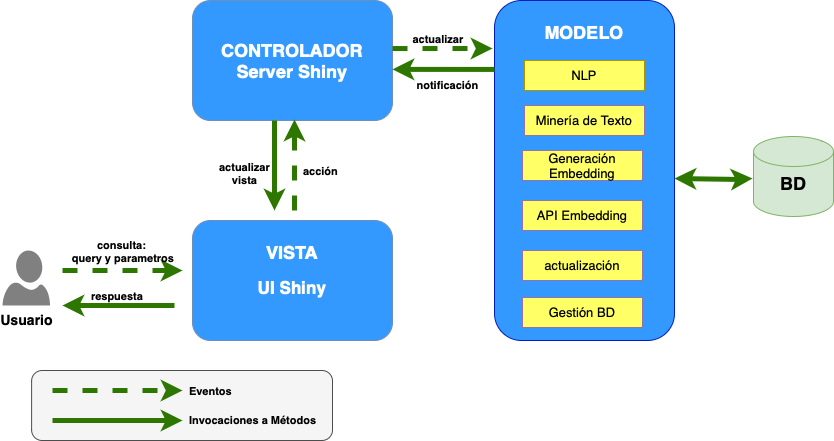
\includegraphics[width=0.9\linewidth]{images/05-desarrollo/MVC9} 

}

\caption{Arquitectura del Sistema}\label{fig:arquitecturasri}
\end{figure}

\hypertarget{justificacion}{%
\section{Justificación e Importancia}\label{justificacion}}

Esta Investigación implementa un método que permite subsanar la falta de clasificaciones por área académica que tiene el repositorio Saber UCV. Adicionalmente, mediante una aplicación web, se amplían los criterios de búsqueda disponibles para investigadores que necesiten realizar consultas sobre los documentos disponibles en el repositorio.

\hypertarget{objegeneral}{%
\subsection{Objetivo General}\label{objegeneral}}

Implementar un sistema de recuperación de información (\emph{information retrieval system}) que realice la extracción y clasificación del cien por ciento de las investigaciones alojadas en el repositorio digital Saber UCV y que este permita efectuar búsquedas de texto empleando un índice invertido y modelos de procesamiento de lenguaje natural.

\hypertarget{objeespe}{%
\subsection{Objetivos Específicos}\label{objeespe}}

\begin{enumerate}
\def\labelenumi{\arabic{enumi}.}
\item
  Conformar un corpus que contenga el cien por ciento de los resúmenes, títulos, palabras claves y nombres de autor, con todos los documentos de tesis doctorales y trabajos de grado de pregrado, maestría y otros documentos alojados en SABER.UCV.
\item
  Clasificar al menos el noventa por ciento de los trabajos de grado alojados en Saber UCV por área académica donde se haya realizado la investigación y extraer en el ochenta por ciento de los documentos el nombre completo del tutor.
\item
  Crear una aplicación web que permita realizar las ``búsquedas de texto completo'' o ``búsqueda semántica'' sobre el corpus conformado, donde se establezcan criterios de relevancia para presentar los resultados de la búsqueda y se representen los ``mapas de conocimiento''.
\item
  Recomendar investigaciones contenidas en el corpus que presenten alguna similitud con cada documento que sea recuperado por el sistema.
\end{enumerate}

\hypertarget{aporte}{%
\section{Aportes}\label{aporte}}

Algunos de los aportes que se generaron al realizar esta investigación son los siguientes:

\begin{itemize}
\item
  Clasificar por área académica un total de 9.585 investigaciones de 9.982 potenciales documentos a categorizar.
\item
  Colocar a disposición de los investigadores un sistema que incrementa los criterios y filtros disponibles para realizar las búsqueda en comparación a los que tiene el repositorio Saber UCV.
\item
  Levantar y procesar un listado con 425 categorías de carreras de pregrado, especializaciones, maestrías y doctorados que se imparten en la Universidad.
\item
  Extraer de los textos de las investigaciones los nombres de los tutores generando un listado con 8.217 nombres y una cantidad de 3.766 nombres únicos.
\item
  Representar mediante mapas de conocimiento interactivos los resultados de las búsquedas.
\item
  Implementar un sistema que permite realizar búsquedas de texto completo y búsquedas semánticas, lo cual se conoce como búsqueda híbrida.
\item
  Integrar un ``sistema de recomendación'' de documentos que presenten similitudes con los textos recuperados.
\item
  Incorporar a los resultados de las búsquedas, gráficos que muestran la evolución histórica de aparición de los términos requeridos.
\item
  Disponer de un sistema que puede integrar publicaciones de otros repositorios de documentos que pertenecen a instituciones nacionales de investigación.
\end{itemize}

\hypertarget{teorico}{%
\chapter{Marco Teórico-Referencial}\label{teorico}}

En este capítulo se exponen los fundamentos teóricos que sustentan los procesos y métodos aplicados en la investigación \textbf{Recuperación, Extracción y Clasificación de Información de SABER UCV}.

\hypertarget{alghist}{%
\section{Reseña histórica}\label{alghist}}

El profesor Donald Knuth señala, dentro del campo de las ciencias de la computación, que la \textbf{búsqueda} ``\emph{es el proceso de recolectar información que se encuentra en la memoria del computador de la forma más rápida posible, esto cuando tenemos una cantidad N de registros y nuestro problema es encontrar el registro apropiado de acuerdo a un criterio de búsqueda''} (\protect\hyperlink{ref-knuth1997}{Knuth 1997, 392}). Este capítulo se inicia con esta cita ya que la recuperación de información gira en torno a un problema central de las ciencias de la computación que es la búsqueda.

En la década de 1940, cuando aparecieron las computadoras, las búsquedas no representaban mayor problema debido a que estas máquinas disponían de poca memoria \emph{RAM} pudiendo almacenar solo moderadas cantidades de datos. No obstante, con el desarrollo e incremento del almacenamiento en memoria \emph{RAM} o en dispositivos de almacenamiento permanentemente, ya en la década de 1950 empezaron a surgir los problemas de búsqueda y consecuentemente las primeras investigaciones para afrontarla.

Fue de esta manera que inicialmente se aplicaron estrategias de ``búsqueda de fuerza bruta'', donde dado un texto \emph{T} y una subcadena \emph{P,} se va recorriendo cada elemento de la cadena \emph{T} para detectar la aparición de la subcadena \emph{P}. Si bien esta estrategia no presentaba el mejor desempeño, sí constituía una forma válida de enfrentar el problema de la búsqueda de subcadenas de texto.

Siguientemente, en la década de 1960 se adoptan estrategias basadas en arboles para resolver los problemas de búsqueda. De los primeros algoritmos que sirvieron para localizar la aparición de una frase dentro de un texto se tienen los de ``\emph{Pattern-Matching}'' (\protect\hyperlink{ref-goodrich2013}{Goodrich, Tamassia, y Goldwasser 2013}).

Avanzando con el recorrido histórico, en 1976 se introdujo el algoritmo ``Knuth-Morris-Pratt\emph{''} que tenía como novedad el que se agregó una función que permitía ir almacenando en una tabla las''previas coincidencias parciales''. Con mayor nivel de detalle, en esta tabla se registraban cuántos caracteres coincidentes se habían encontrado en una posición determinada cuando en la detección del patrón se generaban fallos. Con esto se logró que al momento de realizar un desplazamiento, se tomara en cuenta cuántos caracteres se podían reusar, logrando que se evitara retroceder más allá de lo necesario en el recorrido por la cadena de texto. Fue este enfoque el que permitió mejorar el rendimiento en lo relativo a los tiempos de ejecución comparado con las estrategias citadas previamente.

Seguidamente, en 1977 el problema de la búsqueda se enfrenta con un nuevo algoritmo que es el de ``Boyer-Moore'' en el cual se implementan dos heurísticas denominadas \emph{looking-glass} y \emph{character-jump,} las cuales permiten ir realizando algunos saltos en la búsqueda ante la no coincidencia de la subcadena con la cadena y adicionalmente el orden en el que se va realizando la comparación se invierte, trayendo como consecuencia que se obtuviese un mejor desempeño en el proceso de búsqueda.

Es importante mencionar que, sobre una modificación al algoritmo ``Boyer-Moore'' se sustenta la utilidad \emph{grep} de la línea de comandos UNIX, la cual también da soporte a diversos lenguajes de programación para ejecutar búsquedas de texto, en un proceso que comúnmente es conocido como \emph{grepping}. En particular, esta utilidad fue ampliamente usada para resolver distintos problemas de extracción de información en esta investigación.

Otra de las técnicas a considerar, ya que a ella se acudió para procesar las búsquedas de texto, fue el uso de la programación lineal, donde bajo la premisa ``\emph{divida et impera'',} los problemas que requieren tiempo exponencial para ser resueltos son descompuestos en polinomios y por lo tanto se disminuye la complejidad en tiempo para encontrar la solución.

Dentro de los algoritmos que recurren a la programación lineal está el llamado ``Smith-Waterman'' (\protect\hyperlink{ref-smith1981}{Smith y Waterman 1981}), el cual se desarrolló para efectuar la alineación de cadenas del ADN de forma parcial o total dentro de una cadena mayor. Aunque su uso no estaba destinado a trabajar con caracteres, al poco tiempo de su aparición se identificó que el enfoque que adoptaba era extrapolable a la identificación de subcadenas de texto dentro de una cadena mayor, lo cual motivó a adoptar su uso en los procesos de búsqueda. Es importante señalar que este algoritmo se incorporó con éxito a los métodos implementados en esta investigación para resolver el problema de hacer coincidir las etiquetas de clasificaciones por área académica con el texto de las investigaciones y en el capítulo \ref{desarrollo}, ``Desarrollo de la Solución'', se indicará en detalle cómo fue usado.

Avanzando con el recorrido histórico, corresponde mencionar los algoritmos ``\emph{tries''} (\protect\hyperlink{ref-aho1975}{Aho y Corasick 1975}), en los que se representan los textos mediante estructuras jerárquicas de datos en un árbol compuesto por \emph{tries,} donde se tienen nodos conectados representando cada uno un carácter y de esta manera la ruta desde la raíz hasta un nodo dado, forma una palabra o cadena. Esta estructura permite hacer búsquedas rápidas basadas en patrones y su eficiencia depende de la longitud de la palabra y no del tamaño total del conjunto de datos. Otro elemento a destacar de este algoritmo es que, los textos son sometidos a procesamientos que se hacen previamente a que ocurra el requerimiento de información, con lo cual al momento de hacer la búsqueda ya se dispone de una parte del trabajo realizado y de esta manera, al no tener que ejecutar todo el proceso sobre la marcha, se logran disminuir los tiempos de respuesta.

\hypertarget{infret}{%
\section{Recuperación de Información}\label{infret}}

Christopher Manning, uno de los investigadores con mayor dominio sobre el tema de recuperación de información (RI), la define como el proceso de encontrar materiales que satisfacen una necesidad de información cuando estos se encuentran dentro de grandes colecciones, y generalmente son textos almacenados de forma no estructurada en computadores (\protect\hyperlink{ref-manning2008}{C. D. Manning, Raghavan, y Schütze 2008}). Adicionalmente, el autor Charu Aggarwal menciona que el objetivo que tiene realizar la recuperación de información es conectar la información correcta, con los usuarios correctos en el momento correcto (\protect\hyperlink{ref-miningt2012}{Aggarwal y Zhai 2012}).

En consecuencia, el eje central sobre el cual gira el proceso de recuperación de información es satisfacer las necesidades de información relevante que sean expresadas por un usuario mediante una consulta de texto a la cual se denomina \textbf{\emph{query}}.

En tal sentido, a los efectos de delimitar el espacio de búsqueda sobre el que se realiza la acción de la consulta, se tiene el \textbf{corpus}, al cual se define como el conjunto cerrado de documentos codificados electrónicamente que se encuentra integrado en un sistema de almacenamiento (\protect\hyperlink{ref-martiaurora}{Martín de Santa Olalla Sánchez 1994}) o entendido desde otra perspectiva, es el conjunto de datos en el cual se hará la búsqueda, generando de esta manera el proceso de recuperación de información.

Ahondando un poco más en el tema se tiene que, satisfacer una necesidad de recuperación de información no solo se circunscribe a un problema de búsqueda de un texto dentro de un corpus. En la mayoría de los casos se deberá cumplir con ciertos criterios o restricciones, como por ejemplo, que la aparición del \emph{query} en los documentos esté dentro de un período de fechas o que se encuentre limitado a otras restricciones, siendo esto a lo que se le denomina ``búsqueda multi atributo''.

Por otra parte, dentro de los fundamentos de la RI se tiene que el orden en que sean presentados los distintos documentos recuperados en un proceso de búsqueda, depende de la aparición, parcial o total y de la frecuencia, de las palabras del query dentro de un documento. Lo antes mencionado, junto con otros criterios determina la denominada ``relevancia'', concepto que será abordado con mayor detalle más adelante en \ref{relevancia}, ``Relevancia''.

Adicionalmente, en los procesos de recuperación de información es válido incorporar documentos que no coincidan exactamente con los términos buscados sino otros que contengan palabras que sean sinónimos o que presenten alguna similitud con el texto del \emph{query}. Lo antes mencionado permite incorporar formalmente dentro del proceso de recuperación de información algo de imprecisión con la intención última de enriquecer el proceso (\protect\hyperlink{ref-kraft2017}{Kraft y Colvin 2017}). En \ref{similitud}, ``Similitud de Documentos''\textbf{,} y en \ref{embed}, ``\emph{Embeddings''}\textbf{,} se menciona y especifican algunas de las técnicas con las cuales se incorporan este lote de documentos en los resultados de una búsqueda.

Recapitulando, se tiene que el proceso de recuperación de información está compuesto principalmente por los siguientes elementos:

\begin{itemize}
\item
  Un \emph{\textbf{query}:} el texto a buscar.
\item
  Un \textbf{corpus}: los documentos sobre los cuales se efectuará la búsqueda de información.
\item
  Una función de \textbf{relevancia}: la que permite ordenar los documentos recuperados de mayor a menor importancia para el usuario.
\end{itemize}

\hypertarget{SRI}{%
\subsection{Sistemas de Recuperación de Información (SRI)}\label{SRI}}

Como se vio en la sección anterior, el desarrollo de algoritmos y métodos que permiten realizar procesos de búsqueda, teniendo en paralelo el crecimiento exponencial de datos disponibles en formato digital (\protect\hyperlink{ref-worldde2016}{\emph{World Development Report 2016: Digital Dividends} 2016}), así como también la necesidad de resolver los problemas asociados a la búsqueda con múltiples atributos en tiempos que resulten aceptables, fue lo que abonó las condiciones para la creación de los sistemas de recuperación de información (SRI).

Estos sistemas son los dispositivos (\emph{software} y/o \emph{hardware}) que median entre un potencial usuario que requiere información y la colección de documentos que puede contener la información solicitada (\protect\hyperlink{ref-kraft2017}{Kraft y Colvin 2017}) 1. El SRI se encargará de la representación, el almacenamiento y el acceso a los datos que están estructurados, teniendo presente que las búsquedas que sobre él recaigan conllevan distintos costos, siendo el principal el tiempo que tarde en efectuarse la misma.

Dentro de este contexto, es conocido que los datos estructurados son gestionados mediante un sistema gestor de base de datos, no obstante en el caso de los textos, se manejan por medio de un motor de búsqueda (\emph{search engines}), motivado a que estos en un estado crudo carecen propiamente de estructura (\protect\hyperlink{ref-miningt2012}{Aggarwal y Zhai 2012}). Son estos motores los que permiten que un usuario pueda encontrar fácilmente la información que resulte de utilidad mediante un \emph{query} usando las estructuras de datos, los algoritmos de búsqueda y la aplicación de funciones de relevancia que resulten óptimos para el proceso de recuperación de información.

\hypertarget{ejemplos-de-sri}{%
\subsection{Ejemplos de SRI}\label{ejemplos-de-sri}}

A continuación se referencian dos sitios de internet que funcionan como SRI sobre corpus de investigaciones científicas.

\begin{enumerate}
\def\labelenumi{\arabic{enumi}.}
\item
  Arxiv alojado en \url{https://arxiv.org/}: es un repositorio de trabajos de investigación. Al momento del usuario hacer un requerimiento de información, adicional al texto de la búsqueda, se pueden indicar distintos filtros a aplicar como puede ser el área del conocimiento (física, matemática, computación, etc.), si se quiere ejecutar la busqueda sólo, o de forma combinada dentro de: el título, el nombre autor, el resumen \emph{o} en las referencias.
\item
  Portal de la \emph{Asociation Computery Machine} (ACM) alojado en \url{https://dl.acm.org}: incorpora un motor de búsqueda con particulares características ya que los resultados son acompañados por distintas representaciones gráficas que le dan un valor agregado. En la Figura \ref{fig:busquedasacm}, se ve una de estas representaciones que incluye la frecuencia de aparición de los términos del \emph{query} dentro del corpus en el tiempo.
\end{enumerate}

\begin{figure}

{\centering 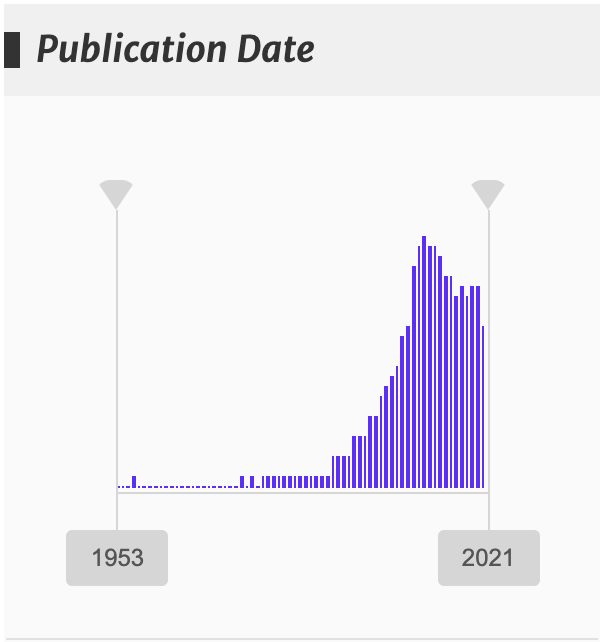
\includegraphics[width=0.3\linewidth]{images/03-marco-teorico/busquedaacm} 

}

\caption{Gráfico que acompaña resultados de búsqueda de un término en la biblioteca digital de la Association for Computing Machinery (https://dl.acm.org/)}\label{fig:busquedasacm}
\end{figure}

\hypertarget{MRI}{%
\subsection{Modelos de Recuperación de Información}\label{MRI}}

\hypertarget{MRIbol}{%
\subsubsection{Recuperación boleana}\label{MRIbol}}

En este modelo ante una búsqueda de información, se recorre linealmente todo el documento para retornar un valor boleano indicando la presencia o no del término buscado. Es uno de los primeros modelos que se usó y está asociado a técnicas de \emph{grepping} (\protect\hyperlink{ref-manning2008}{C. D. Manning, Raghavan, y Schütze 2008}). El desarrollo de este modelo apareció entre 1960 y 1970.

El ojetivo planteado por este modelo es que el usuario final obtenga como respuesta a un \emph{query} solo aquellos textos que contengan el término. Es un modelo muy cercano a los típicos \emph{queries}de bases de datos con el uso de operadores lógicos ``\emph{AND}'', ``\emph{OR}'' y ``\emph{NOT}''.

Especificamente, el modelo ``booleano'' en el procesamiento de los textos genera una matriz de incidencia binaria término-documento, donde cada término que conforma el vocabulario, ocupa una fila \emph{i} de la matriz, mientras que cada columna \emph{j} se asocia a un documento. La presencia del término \emph{i} en el documento \emph{j} se denotará con un valor verdadero o un ``1''.

De acuerdo a lo anterior, la recuperación boleana si bien representa una buena aproximación al procesamiento de \emph{queries}con mayor rapidez, también hace que se presente una gran desventaja y es que al crecer la cantidad de documentos, junto con el vocabulario (palabras únicas contenidas dentro del corpus), se obtiene una matriz dispersa de una alta dimensionalidad que hace poco efectiva su implementación.

Igualmente, las deficiencias de este modelo también reacaen en que los resultados que se obtienen ante una búsqueda no tienen representado ningún criterio de relevancia. Si por ejemplo, el término sobre el cual se realiza el \emph{query} aparece 100 veces en un documento y en otro solo aparece una vez, en la presentación de los resultados ambos documentos se mostrarán al mismo nivel, no pudiendo indicar la mayor relevancia que puede tener uno sobre el otro.

De la misma forma, también se tiene como otra de desventaja que en este modelo no se registra el contexto semántico de las palabras e incluso se pierde el orden en que aparecen los términos dentro de cada texto.

\hypertarget{invind}{%
\subsubsection{Índices Invertidos}\label{invind}}

Es ampliamente conocido el proceso de indexación como aquel en el cual se generan índices dentro de las bases de datos, sin embargo, en los sistemas de recuperación de información se genera otro tipo de índice que recibe el nombre de ``índice invertido''. En él, en vez de guardar los nombres de los documentos junto con las palabras que aparecen, se procede a registrar en una lista cada palabra y a continuación se indican los nombres o se guardan apuntadores a los documentos en los cuales se encuentra la misma. Adicionalmente, también se puede registrar la posición en que aparece cada una de estas, relativo a algún criterio, como puede ser el inicio del documento o del párrafo. Igualmente se puede registrar la frecuencia con que se presenta cada término en el documento.

De esta manera, se tiene que cuando un SRI funciona mediante un índice invertido, esto conlleva a que se puedan realizar las denominadas ``búsquedas de texto completa'' (\emph{full text search}) así como también a realizar las búsquedas de texto aproximado \emph{(approximate text searching)}, donde se flexibiliza la coincidencia entre el texto requerido y el resultado.

No obstante, hay que tener presente que la creación del índice inverso conlleva a algunos costos computacionales, siendo el primero de estos el mayor espacio de almacenamiento que se consume al guardar estos datos adicionales, incrementando el tamaño del registro de un 5\% al 100\% del valor inicial, según las configuraciones que se decida adoptar al crearlo. El segundo costo a tener en cuenta está determinado por los cálculos informáticos que se deben hacer al momento de actualizar el índice, una vez que se incorporan nuevos documentos (\protect\hyperlink{ref-Mahapatra2011}{Mahapatra y Biswas 2011}). En el capítulo \ref{desarrollo}, ``Desarrollo de la Solución'', se indicará en cuánto se incrementó el espacio de almacenamiento en disco con la generación de el índice inverso del SCSU.

La situación expuesta motiva a que existan diversos tipos de índices invertidos y a que constantemente se estén realizando investigaciones que permitan mejorar su desempeño, motivado a que sobre ellos recae, en gran parte, la efectividad que se puede obtener ejecutando los \emph{querys}. Algunos ejemplos de estos índices son el \emph{Generalized Inverted Index} (GIN), RUM \footnote{En el vínculo \url{https://github.com/postgrespro/rum} se tiene acceso a la explicación e implementación de este índice para PostgreSQL.} y VODKA \footnote{este índice fue presentado en la Postgres Conference en el año 2014 \url{https://www.pgcon.org/2014/schedule/attachments/318_pgcon-2014-vodka.pdf}} y en el trabajo de (\protect\hyperlink{ref-Mahapatra2011}{Mahapatra y Biswas 2011}) se encuentran detalles adicionales sobre ellos.

En contraparte, el espacio de almacenamiento que ocupa la implementación de estos índices se puede ver reducido mediante el preprocesamiento que se haga a las palabras buscando las raices de ellas, siendo uno de los métodos usados la aplicación del \emph{stemming}, el cual se expondrá más adelante o también mediante la remoción de las \emph{stopwords}, que son las palabras que no aportan mayor valor semántico dentro de un texto, como pueden ser los términos: la, el, tu, ella, son, entre varios otros.

Siguiendo adelante en el tema, existen estrategias de implementación de un sistemas de recuperación de información donde se generan dos o más índices inversos, conteniendo, por ejemplo, uno de estos la lista de documentos y la frecuencia de la palabra, mientras que en el otro se registra la lista con las posiciones de la palabra.

Para finalizar lo referente a los índices invertidos, se tiene que cuando la base de datos en que se soporta el sistema de recuperación de información crece y no es viable almacenarla en un único computador, es necesario acudir al uso de algoritmos y tecnologías que permitan distribuir los datos en sistemas distribuidos y paralelos como pueden ser Spark, Hadoop o Apache Storm.

\hypertarget{relevancia}{%
\subsection{Relevancia}\label{relevancia}}

Refiere la medida en que un documento o recurso recuperado satisface las necesidades de información del usuario. En otras palabras, un documento es relevante si contiene información que es útil y está relacionada con el \emph{query} realizado por el usuario (\protect\hyperlink{ref-buxfcttcher2010a}{Büttcher, Clarke, y Cormack 2010a}). La relevancia no es una propiedad intrínseca del documento, sino que depende del contexto y de las necesidades de información del usuario en un momento específico.

De esta manera, para establecer la relevancia que presente un documento sobre los otros, se usan distintos métodos, los cuales también han variado según las representaciones computacionales que se hagan de los textos. Bajo el modelo de recuperación boleano se puede dar un mayor peso a la aparición de la frase del \emph{query} dentro del título de un texto o en las palabras clave. Otro método que se adopta es determinar la proximidad o cercanía entre las palabras contenidas en el texto recuperado, según la condición que establece el \emph{query}. También se acude a realizar el cálculo de la frecuencia de aparición de una palabra, o varias, dentro del documento y su relación con el \emph{query}, dando una mayor jerarquía a aquellos documentos que presenten una frecuencia de aparición mayor de los términos.

También se tiene que, otro método usado para establecer la relevancia, es determinar las referencias (citas), que contengan otros documentos a ese determinado escrito, similar a la propuesta del algoritmo \emph{PageRank} (\protect\hyperlink{ref-brin1998}{Brin y Page 1998}).

Recientemente, una de las propuestas adoptadas para establecer los criterios de relevancia es efectuar la comparación vectorial, detallada en \ref{similitud}, ``Similitud de Documentos'' , de los \emph{embeddings}, por definir en \ref{embed}, ``\emph{Embeddings}'', que generan frases de un documento dentro del corpus con el \emph{embedding} generado desde la frase del \emph{query}.

\hypertarget{ranking}{%
\subsection{Re Ordenamiento (re-ranking)}\label{ranking}}

Es una técnica utilizada para mejorar la precisión y lograr extraer los documentos que tengan mayor relevancia en los resultados de una búsqueda.

Cuando los usuarios realizan el \emph{query} a menudo se encuentran con una gran cantidad de documentos que coinciden con sus consultas, sin embargo, no todos estos documentos son igualmente relevantes para el usuario. El \emph{re-ranking} implica reorganizar los resultados de búsqueda originales para que los documentos más relevantes aparezcan en las primeras posiciones, mejorando así la experiencia del usuario.

Cabe destacar que, en algunos casos el sistema de recuperación de información en la función de relevancia ejecuta el proceso de reordenamiento mientras que en otros este proceso es ejecutado con un método distinto que puede estar basado en técnicas soportadas en aprendizaje automático.

\hypertarget{learning-to-rank-ltr}{%
\subsubsection{Learning to Rank (LTR)}\label{learning-to-rank-ltr}}

Los algoritmos de aprendizaje para la clasificación (LTR, por sus siglas en inglés) son comúnmente utilizados para el re-ranking. En ellos se utilizan técnicas de aprendizaje automático para modelar la relevancia de los documentos basándose en características específicas (\protect\hyperlink{ref-buxfcttcher2010}{Büttcher, Clarke, y Cormack 2010b}). Los atributos pueden incluir la frecuencia de palabras clave, la proximidad de términos en el documento y otros factores que indican la relevancia.

El siguiente aspecto a considerar es que los modelos LTR pueden ser entrenados con conjuntos de datos que contienen consultas y documentos etiquetados con su relevancia, y luego aplicados para re-ordenar los resultados de búsqueda en función de las características aprendidas.

\hypertarget{bm25}{%
\subsubsection{BM25}\label{bm25}}

Es un algoritmo que apareció a mediados de la década de 1990 y contiene una función matemática compleja de puntuación basada en un modelo probabilístico (\protect\hyperlink{ref-zhai2016}{Zhai y Massung 2016}) la cual es utilizada para calcular la relevancia de un documento con respecto a una consulta (\protect\hyperlink{ref-robertson2009}{Robertson y Zaragoza 2009}) determinando la frecuencia de aparición de los términos de la búsqueda junto con la longitud del documento. Ha demostrado ser efectivo en la práctica para clasificar documentos según la relevancia que estos presenten, llegando en algún momento a decirse que obtenía un rendimiento similar al de un humano experto al hacer el proceso que de jerarquización en el proceso de recuperación de información.

\hypertarget{evaluacion}{%
\subsection{Medidas y Métodos de Evaluación de Desempeño de los SRI}\label{evaluacion}}

Las siguientes métricas son usadas en el campo de la recuperación de información para evaluar el desempeño de un SRI:

\begin{enumerate}
\def\labelenumi{\arabic{enumi}.}
\item
  \textbf{Exactitud (\emph{accuracy}):} mide la proporción de documentos relevantes recuperados por el sistema con respecto al total de documentos recuperados.
\item
  \textbf{Precisión \emph{(precision)}:} es la proporción de documentos relevantes recuperados por el sistema con respecto a todos los documentos recuperados. Cuanto mayor es la precisión, menos documentos irrelevantes se recuperan.
\item
  \textbf{Recuperación (\emph{recall}} \textbf{):} es la proporción de documentos relevantes recuperados por el sistema con respecto a todos los documentos relevantes presentes en la base de datos. Un alto ``recall'' indica que el sistema encuentra la mayoría de los documentos relevantes.
\item
  \textbf{\emph{F1 Score}:} es la media armónica de la precisión (\emph{precision)} y la recuperación (\emph{recall)}. Esta medida proporciona un equilibrio entre los resultados que aportan las dos medidas que tiene de insumo. Un \emph{F1 Score} alto indica un buen equilibrio entre la precisión y la capacidad para encontrar todos los documentos relevantes.
\end{enumerate}

Una vez enunciados los conceptos de estas tres medidas es necesario determinar el proceso con que se puede determinar la ``relevancia'' de los documentos recuperados por un SRI. Para explicar esto se expondrá brevemente el origen de este método.

Posterior a la segunda guerra mundial, se incrementó considerablemente la publicación de investigaciones en el ámbito científico y se hizo necesario contar con sistemas analógicos que fuesen eficientes para la indexación de los documentos. En el estudio denominado ``\emph{Cranfield Tests}'' (\protect\hyperlink{ref-harman2011}{Harman 2011}), que fue conducido por Cyril Cleverdon, a partir de 1958 se empezaron a definir los estándares para evaluar la efectividad de los índices disponibles para aquel momento.

Para ese entonces se definió la ``relevancia'' como lo que lo que actualmente se conoce como ``exactitud'' y la estrategia que se adoptó para poder determinarla fue usar el \emph{``known-item searching''} (búsqueda del elemento conocido), que consistía en encontrar un documento que garantizara ser relevante ante una determinada pregunta. Para obtener la dupla ``pregunta - identificación del documento con respuesta correcta'' , acudieron a los autores de 1.500 trabajos y les pidieron que formulasen una pregunta que satisfactoriamente iba a ser respondida en el texto de su autoría (\protect\hyperlink{ref-harman2011}{Harman 2011}).

Avanzando en el tiempo tenemos que desde inicios de la década de 1990, con las reuniones periódicas de la denominada ``\emph{Text Retrieval Evaluation Conference}-TREC'', se crean distintos conjuntos de datos con diversos documentos agrupados por temas donde expertos anotan con una expresión binaria: ``relevante'' o ``no relevante'', los juicios de relevancia para así poder indicar cuáles son los documentos más destacados para cada uno de los tópicos.

Es por esta razón que los conjuntos de datos constituidos por la dupla antes detallada, se les llama ``\emph{standard test collections}'', ``\emph{golden standard}'' o ``\emph{ground truth judgment of relevance}'' (juicio de pertinencia basado en la verdad). Contar con estas colecciones permitió diseñar un método para poder evaluar el desempeño de un sistema al ejecutar el proceso de generación de ``relevancia'', comparando el criterio de los expertos con el obtenido desde el sistema.

No obstante, el problema que presenta el enfoque mencionado es que ante métodos de recuperación de documentos más avanzados, como la búsqueda semántica, la cual será presentada en \ref{busquedasemantica}, ``Búsqueda Semántica'', así como con la aparición de temas de investigación más especializados y también ante el incremento de documentos digitales, este tipo de mediciones se queda un tanto rezagada y no muestra la real efectividad en los procesos de RI que pueden disponer los sistemas.

Igualmente es necesario señalar que, las medidas ``\emph{precisión}''y ``\emph{recall''} en algunos casos no llegan a reflejar la verdadera satisfacción del usuario, ya que el diseño de la interfaz del sistema afecta positiva o negativamente, lo que realmente debe ser la medición de la relevancia que dispone el SRI sometido a evaluación (\protect\hyperlink{ref-manning2008}{C. D. Manning, Raghavan, y Schütze 2008}).

\hypertarget{PT}{%
\section{Procesamientos a los textos}\label{PT}}

En esta sección se exponen diversos métodos que comúnmente se usan para procesar textos, teniendo presente que son estos el insumo con el cual se conforma el corpus anotado (\protect\hyperlink{ref-desagulier2017}{Desagulier 2017}) de cualquier SRI y que efectuar óptimas manipulaciones sobre los documentos determinará en gran medida la propia calidad del sistema que se obtenga.

Primero que todo, es necesario contextualizar que la aplicación de las técnicas que serán revisadas tienen absoluta dependencia del idioma usado a diferencia de procesamientos que se pueden hacer a otros tipos de datos. Las herramientas que se seleccionan van a analizar, categorizar y extraer información de las palabras y oraciones para poder obtener estructuras gramaticales y morfológicas, haciendo que estos recursos estén directamente asociados a la lengua que posean los textos.

En tal sentido, previo al año 2016 eran escasas las herramientas computacionales para la manipulación de documentos en el idioma español. Los \emph{frameworks} disponibles para realizar las tareas de procesamiento, se sustentaron en la adopción de las bases que da el proyecto \emph{``Universal Dependencies''} (\protect\hyperlink{ref-demarneffe2021}{Marneffe et~al. 2021}), tal es el caso del ``coreNLP'' de la Universidad de Stanford (\protect\hyperlink{ref-manning-etal-2014-stanford}{C. Manning et~al. 2014}), que fue uno de los primeros en incluir dos métodos para el procesamiento de los textos con su tokenizador y también con el separador de oraciones (\emph{sentences splitting}), sin disponer de otras utilidades como la identificación de las parte del discurso (\emph{part of speech tagging),} el análisis morfológico (\emph{morphological analysis)} (\protect\hyperlink{ref-straka2017}{Straka y Straková 2017}) o el reconocimiento de entidades nombradas (\emph{named entity recognigtion),} que sí se encontraban disponibles para el idioma inglés.

Sin embargo, un caso aparte para la época, es el esfuerzo de la Universidad Politécnica de Cataluña quienes crearon la herramienta \emph{FreeLing} \footnote{\url{https://nlp.lsi.upc.edu/freeling/node/1}}, la cual tuvo como entrada de datos para el entrenamiento del modelo el Corpus AnCora \footnote{\textbf{AnCora} es un corpus del \textbf{catalán (AnCora-CA)} y del \textbf{español (AnCora-ES)} con diferentes niveles de anotación como lema y categoría morfológica, constituyentes y funciones sintácticas, estructura argumental y papeles temáticos, clase semántica verbal, tipo denotativo de los nombres deverbales, sentidos de WordNet nominales, entidades nombradas (NER), relaciones de correferencia (\url{http://clic.ub.edu/corpus/es/ancora})} anotado por el ``\emph{CLiC- Centre de Llenguatge i Computación}''. Este software. soportado en un modelo de aprendizaje automático, fue uno de los primeros en poner a disposición de los usuarios de textos en español, la identificación de las parte del discurso y el análisis morfológico de las palabras.

Con el trancurrir del tiempo, este proyecto fue desplazado ya que otros \emph{frameworks} con mejores integraciones de cadenas de trabajo (\emph{pipelines}), así como el uso de otras arquitecturas de modelos de redes neuronales más potentes (\protect\hyperlink{ref-chen2014fast}{Chen y Manning 2014b}), permitieron la aparición de diversas herramientas que sí dieron soporte a la lengua española hacia finales de la década del 2010. En la sección \ref{sota}, ``Estado del Arte'', se revisaran algunos de estos avances.

\hypertarget{nlproc}{%
\subsection{Procesamiento del Lenguaje Natural (Natural Language Processing- NLP)}\label{nlproc}}

El procesamiento del lenguaje natural (PNL) es el conjunto de técnicas computacionales desarrolladas para permitir al computador representar e interactuar de una forma más efectiva con los textos. La \emph{tokenización}, el etiquetado de partes del discurso, el \emph{stemming} y la \emph{lematización} son algunos de los métodos que lo componen. Es necesario destacar que cada uno de los métodos que se detallan a continuación fueron aplicados sobre el corpus del SCSU.

\hypertarget{token}{%
\subsubsection{Tokenizador}\label{token}}

Básicamente un tokenizador es una herramienta que permite separar un documento en palabras, o unidades semánticas que tengan algún significado. Las unidades obtenidas se les llama \emph{tokens} (\protect\hyperlink{ref-straka2017}{Straka y Straková 2017}).

En complemento de lo anterior, realizar este procesamiento para el idioma español no representa un mayor reto, ya que generalmente se puede usar el espacio como delimitador de palabras, no así en otros idiomas como el chino donde el problema se aborda de manera distinta.

De esta forma, al obtener las palabras como entidades separadas de un texto se permite, por ejemplo, calcular la frecuencia de uso de las mismas dentro del corpus.

En este contexto, las librerías de procesamiento de lenguaje natural para el idioma español disponen de tokenizadores que comúnmente presentan un 100\% de precisión en la ejecución de separar las palabras.

Igualmente hay que destacar que los tokenizadores que se usan para generar \emph{embedding}s, ver \ref{embed}, ``\emph{Embeddings}'', tienen un comportamiento distinto al hacer la separación de las unidades que conforman el texto basándose en reglas.

\hypertarget{pos}{%
\subsubsection{\texorpdfstring{Etiquetado de Partes del Discurso \emph{(Part of speech tagging-POS)}}{Etiquetado de Partes del Discurso (Part of speech tagging-POS)}}\label{pos}}

Consiste en asignar un rol sintáctico a cada palabra dentro de una frase (\protect\hyperlink{ref-eisenstein2019}{Eisenstein 2019}), siendo necesario evaluar cómo cada palabra se relaciona con las otras que están contenidas en una oración y así se revela la estructura sintáctica.

En este sentido, los roles sintácticos principales de interés en la elaboración de esta investigación son los sustantivos, adjetivos y verbos. Al recordar muy brevemente cuáles son estos roles se tiene que:

\begin{itemize}
\item
  Los sustantivos tienden a describir entidades y conceptos.
\item
  Los verbos generalmente señalan eventos y acciones.
\item
  Los adjetivos describen propiedades de las entidades.
\end{itemize}

Igualmente, dentro del POS se identifican otros roles sintácticos como los adverbios, nombres propios, interjecciones, por solo mencionar algunos.

En específico, en esta investigación la ejecución del POS permite que se obtenga una tabla que sirve de insumo para determinar la coocurrencia de palabras, que es una de las formas en que se representan los resultados de los \emph{queries}en el sistema desarrollado.

Se destaca que en el estado del arte, este proceso de etiquetado para el idioma español alcanza un 98\% de precisión.

\hypertarget{steaming}{%
\subsubsection{\texorpdfstring{\emph{Stemming}}{Stemming}}\label{steaming}}

El \emph{Stemming} es un algoritmo que persigue encontrar la raíz de una palabra, teniendo como el de mayor uso el Algoritmo de Porter (\protect\hyperlink{ref-willett2006}{Willett 2006}). Al ser usado se puede reducir considerablemente el número de palabras que conforman el vocabulario del corpus y así consecuentemente mejorar los tiempos en que se ejecuta la búsqueda de un texto, ya que se disminuye el espacio de búsqueda.

Sin embargo, se hace la consideración de que al aplicar este algoritmo, no se toma en consideración el contexto en el que aparece la palabra a la que se le extrae la raíz. Como ejemplo se muestra que ``yo canto, tú cantas, ella canta, nosotros cantamos, ellos cantan'' en todos los casos se tendrá como raíz la cadena de letras (ref:letras)

Finalmente, es necesario tener presente que al crear el índice invertido son las raíces de las palabras las que se guardarán y no propiamente la palabra que aparece en el texto.

\hypertarget{lemma}{%
\subsubsection{Lematización}\label{lemma}}

Es el proceso con el cual se consigue el \emph{lema} de una palabra, entendiendo que el \emph{lema} es la forma que por convenio se acepta como representante de todas las formas flexionadas de una misma palabra (\protect\hyperlink{ref-demarneffe2021}{Marneffe et~al. 2021}). Los lemas, o lexemas, constituyen la parte principal de la palabra, la que transmite el significado. Los morfemas son el elemento variable de la palabra y son los que se busca desechar en el proceso de lematización.

En este sentido, al buscar el \emph{lema} se tiene presente la función sintáctica que tiene la palabra, es decir que se evalúa el contexto en el que ocurre. Una de las ventajas de aplicar esta técnica es que se reduce el vocabulario del corpus y eso conlleva a que también se reduzca el espacio de búsqueda. Un ejemplo de lematización se puede representar con estas tres palabras: ``bailaré, bailamos, bailando'' que tienen el mismo \emph{lema} que es ``bailar''.

Una consideración final sobre este tema es que, en el estado del arte este proceso alcanza un 96\% de precisión en varios de los modelos de aprendizaje automático preentrenados, no obstante no se disponen datos puntuales de esta métrica para el idioma español.

\hypertarget{textmin}{%
\subsection{Minería de Texto}\label{textmin}}

La extracción de ideas útiles derivadas de textos mediante la aplicación de algoritmos estadísticos y computacionales se conoce con el nombre de minería de texto (\emph{text mining)}, analítica de texto (\emph{text analytics)} o aprendizaje automático para textos \emph{(machine learning from text}). Se quiere con ella representar el conocimiento en una forma más abstracta y así poder detectar relaciones y patrones en los textos (\protect\hyperlink{ref-aggarwal2018a}{Aggarwal 2018a}).

De esta manera se tiene que, la minería de texto surge para dar respuesta a la necesidad de tener métodos y algoritmos que permitan procesar estos datos no estructurados (\protect\hyperlink{ref-miningt2012}{Aggarwal y Zhai 2012}) y ella ha ganado atención en recientes años motivado a las grandes cantidades de textos digitales que están disponibles. Los procesamientos inherentes al NLP mencionados anteriormente son insumo para la minería de texto.

A continuación se procede a exponer algunos de los métodos que pertenecen a la minería de texto:

\hypertarget{tdm}{%
\subsubsection{Term-Document Matrix}\label{tdm}}

Una vez que se tiene conformado un corpus, se procede a conformar una matriz dispersa de una alta dimensionalidad que se denominará \emph{``Sparce Term-Document Matrix)''} de tamaño \emph{n X d,} donde \emph{n} es el número total de documentos y \emph{d} es la cantidad de términos o vocabulario (palabras distintas) presentes entre todos los documentos. Formalmente se sabe que la entrada \emph{(i,j)} de nuestra matriz es la frecuencia (cantidad de veces que aparece) de la palabra \emph{j} en el documento \emph{i}. Este procedimiento es similar al que fue revisado en \ref{MRIbol}, ``Recuperación Boleana''.

Cabe destacar, que uno de los problemas que presenta la matriz obtenida es la alta dimensionalidad y lo dispersa que es, llegando a estar conformada en un 98\% por ceros, los cuales indican la ausencia de aparición de una palabra en un determinado documento.

Sin embargo, para mejorar un tanto este tipo de representación del corpus, se aplican otras técnicas que en principio puedan colaborar a reducir la dimensionalidad, por medio de simplificar los atributos, es decir, disminuyendo el vocabulario aplicando el stemming como se vio anteriormente.

\hypertarget{coocurrencia}{%
\subsubsection{Coocurrencia de Palabras}\label{coocurrencia}}

En esta investigación, se usa un método denominado ``coocurrencia de palabras'' para la detección de patrones en los textos y se hará la representación de aparición de las coocurrencias mediante grafos. El método se explica en que se evalúan las palabras que coocurren, es decir, aquellas que forman parte del conjunto de palabras obtenidas de la intersección de los documentos que conforman el corpus\emph{,} o del subconjunto de documentos recuperados mediante un determinado \emph{query}.

Adicionalmente, se tiene que se puede establecer el nivel al que se quiere determinar la coocurrencia, por ejemplo, las palabras que coocurren una seguida de otra en los textos, las que coocurren dentro de la misma oración, dentro de un párrafo o dentro de todo el texto de cada documento.

Por otra parte, para la representación de las coocurrencias se usan grafos, donde cada palabra se representa un nodo y la coocurrencia de una palabra con otra implica que se extienda un arco entre ellas. Las palabras dispuestas para representarse en el grafo serán exclusivamente las que tengan la función dentro del discurso (POS) de adjetivos y sustantivos, es decir que cada coocurrencia será un sustantivo con el adjetivo que la acompaña, donde es posible tener una relación de 1 sustantivo con un conjunto de \{0,1,\ldots,n\} adjetivos. Para lograr esto, la selección de las funciones gramaticales propuestas se hace para disminuir el espacio de representación y se considera que los sustantivos, al contar con el adjetivo que las acompaña, logran hacer una representación que muestra proximidad semántica y se representan los tópicos más relevantes (\protect\hyperlink{ref-segev2021}{Segev 2021}).

En la Figura\ref{fig:coocejem}, se visualiza lo expuesto de una manera gráfica, al ver la representación en un grafo la coocurrencia de palabras sobre los textos de los resúmenes de las tesis y trabajos especiales de grado de la Escuela de Física de la U.C.V.

\begin{figure}

{\centering 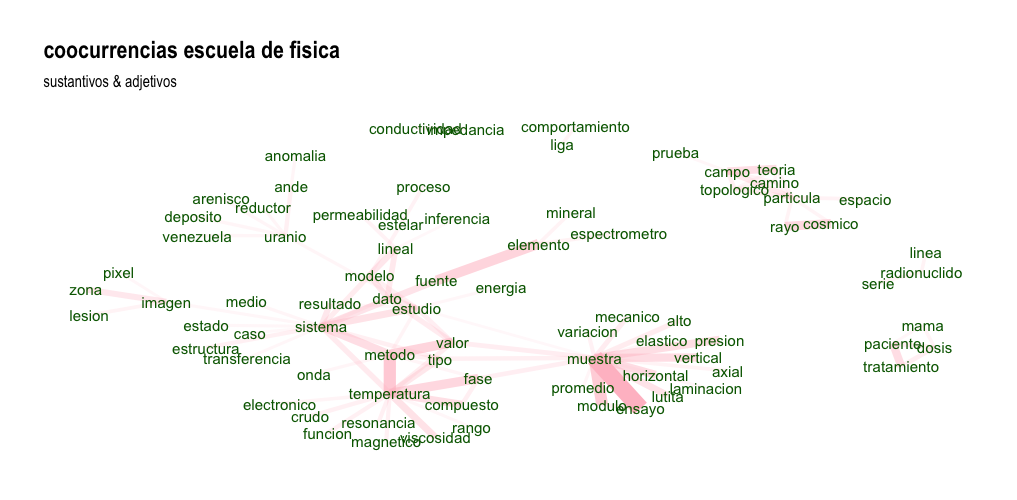
\includegraphics[width=0.9\linewidth]{images/03-marco-teorico/cooc} 

}

\caption{Coocurrencia de palabras}\label{fig:coocejem}
\end{figure}

\hypertarget{mapacon}{%
\paragraph{Mapas de Conocimiento}\label{mapacon}}

La representación gráfica y el método de extracción de sustantivos y adjetivos, toma como referencia la investigación ``Propuesta Metodológica para Realizar Mapas de Conocimiento'', (\protect\hyperlink{ref-dueuxf1as2011}{Dueñas, Rojas, y Morales 2011}) para crear ``mapas de conocimiento'' con ``las palabras claves obtenidas a través de búsquedas recurrentes y relacionadas''. En esta investigación se simplificará la obtención y representación de estos mapas, asumiendo que las palabras clave son los sustantivos adjetivizados, equivalente a visualizar las personas, cosas o ideas que se mencionan y que son modificados por los adjetivos, al cambiar sus propiedades o atributos; seleccionando aquellas palabras que muestran una mayor aparición en el \emph{query} realizado y que se interconectan en un grafo mediante arcos.

\hypertarget{similitud}{%
\subsection{Similitud de Documentos}\label{similitud}}

Para poder realizar la recomendación de documentos, una de las técnicas que se usa es medir la similitud que presenta un documento con los otros contenidos en el corpus (\protect\hyperlink{ref-aggarwal2018a}{Aggarwal 2018a}). Un ejemplo de esta técnica es el uso de la similitud coseno que se explica con esta fórmula.

\begin{equation}
\cos ({\bf t},{\bf e})= {{\bf t} {\bf e} \over \|{\bf t}\| \|{\bf e}\|} = \frac{ \sum_{i=1}^{n}{{\bf t}_i{\bf e}_i} }{ \sqrt{\sum_{i=1}^{n}{({\bf t}_i)^2}} \sqrt{\sum_{i=1}^{n}{({\bf e}_i)^2}} }
\end{equation}

En este sentido, en la fórmula, \emph{t} representa un documento y \emph{e} representa otro documento. Ambos documentos se asumen que están en un espacio con \emph{i} atributos, o dimensiones, y la intención es calcular un índice de similitud entre ambos documentos. En este orden de ideas se tiene que este es uno de los métodos más usados para detectar similitudes en los textos, aunque existen otras fórmulas para el cálculo de la similitud como lo es el índice de Jaccard.

Adicionalmente se tiene que, hacer la comparación de un documento \emph{i} del corpus que contiene \emph{n} documentos, en un proceso iterativo con otra cantidad de (\emph{n-1)} documentos, de se se obtienen (\emph{n-}1) índices de similitud. Aquel que obtenga un mayor valor se puede inferir que presenta una mayor similitud con el documento \emph{i.}

En el mismo orden de ideas se tiene que, otro elemento de gran importancia a evaluar en el resultado que se obtiene de esta medición, es la representación computacional que se haga del documento. Son distintas las técnicas que existen, estando entre ellas la representación mediante ``bolsas de palabras'' o \emph{bag of words,} similar a lo que se explicó en \ref{tdm}, ``\emph{Term Document Matrix}'', donde un documento \emph{i} es el vector correspondiente a una fila de la matriz y la cantidad de dimensiones que presenta es equivalente al tamaño del vocabulario.

Un elemento importante a destacar de realizar este tipo de comparaciones, la estimación de la similitud, es que ante un proceso de \emph{query} también pueden ser recuperados, o sugerir al investigador, aquellos documentos que presenten alguna mínima similitud con los documentos recuperados.

Finalmente, se procede a resaltar que recientemente se han creado formas más complejas para la representación de los documentos, como lo son los \emph{word embeddings} que son obtenidos mediante el entrenamiento de redes neuronales de aprendizaje profundo, lo que será expuesto en \ref{embed}, ``\emph{Embeddings}''.

\hypertarget{SD}{%
\section{Sistemas Distribuidos}\label{SD}}

Los distintos procesos y componentes de la solución propuesta han sido diseñados e implementados como un sistema distribuido y por eso se hace la mención a este tema.

En tal sentido, una definición formal que se le puede dar a los sistemas distribuidos es ``cuando los componentes de hardware y/o software se encuentran localizados en una red de computadores y estos coordinan sus acciones solo mediante el pase de mensajes'' (\protect\hyperlink{ref-distribu2012}{Coulouris 2012}).

De acuerdo a lo anterior, se tiene que algunas de las principales características que poseen los sistemas distribuidos es la tolerancia a fallos, compartir recursos, concurrencia, ser escalables (\protect\hyperlink{ref-czaja2018}{Czaja 2018}) entre otras. Mencionamos estas, en particular, al ser propiedades que están presentes en la solución que se implementa:

\begin{enumerate}
\def\labelenumi{\arabic{enumi}.}
\item
  Fiabilidad (tolerancia a fallos): al fallar un componente del sistema los otros se deben mantener en funcionamiento.
\item
  Compartir recursos: un conjunto de usuarios pueden compartir recursos como archivos o base de datos.
\item
  Concurrencia: poder ejecutar varios trabajos en simultáneo.
\item
  Escalable: al ser incrementada la escala del sistema se debe mantener en funcionamiento el sistema sin mayores contratiempos.
\end{enumerate}

\hypertarget{contenedores}{%
\subsection{Contenedores}\label{contenedores}}

Un contenedor es una abstracción de una aplicación que se crea en un ambiente virtual, en el cual se encuentran ``empaquetados'' todos los componentes (sistema operativo, librerías, dependencias, etc.), que una aplicación necesita para poder ejecutarse. En su diseño se tiene presente que sean ligeros y que con otros contenedores pueden compartir el \emph{kernel}, usando un sistema de múltiples capas, que también pueden ser compartidas entre diversos contenedores, ahorrando espacio en disco del \emph{host} donde se alojan los contenedores (\protect\hyperlink{ref-nuxfcst2020}{Nüst et~al. 2020}).

De lo indicado en el punto anterior se tiene que, el uso de los contenedores permite crear, distribuir y colocar en producción aplicaciones de software de una forma sencilla, segura y reproducible. También a cada contenedor se le puede realizar una asignación de recursos (memoria, CPU, almacenamiento) que garantice un óptimo funcionamiento de la aplicación que contienen. Es importante señalar que, el uso de esta tecnología también añade un entorno de seguridad al estar cada contenedor en una ambiente isolado.

Igualmente hay que resaltar que, para instanciar cada contenedor es necesario disponer de una imagen donde previamente se definen las dependencias (sistema operativo, librerías, lenguajes) necesarias para su funcionamiento.

\hypertarget{orquestador}{%
\subsection{Orquestadores}\label{orquestador}}

Cuando se tienen diversos contenedores para sustentar un sistema, donde cada uno aloja una aplicación o servicio distinto, puede resultar necesario que todos se integren y compartan recursos optimizadamente. Para que esta integración sea viable es necesario contar con un orquestador (\protect\hyperlink{ref-cook2017}{Cook 2017}). Su uso permitirá lograr altos grados de portabilidad y reproducibilidad, pudiendo colocarlos en la nube o en centros de datos, garantizando que se pueda hacer el \emph{deploy} de forma sencilla y fiel a lo que se implementó en el ambiente de desarrollo.

Así mismo, en el caso de la solución propuesta se adoptará el uso de \emph{Docker Compose} como orquestador y en el capítulo \ref{desarrollociclos4}, ``Ciclos de Desarrollo'', serán expuestas las funcionalidades de cada contenedor y del orquestador.

\hypertarget{sota}{%
\section{Estado del Arte}\label{sota}}

Si bien anteriormente las búsquedas de información dentro de un corpus se procesaban determinando la aparición de palabras dentro de un texto, este método ha ido evolucionando, pasando de tener motores de búsqueda (\emph{search engines}) a los denominados motores de respuestas (\emph{answering engines}) (\protect\hyperlink{ref-balog2018}{Balog 2018}), donde el sistema ante una determinada consulta va a retornar una serie de resultados enriquecidos, mostrando la identificación de entidades, hechos y cualquier otro dato estructurado que esté de forma explícita e implícita, mencionado dentro de los textos que conforman el corpus.

Es por esto que, para hablar sobre el estado del arte tanto en los sistemas de recuperación de información, así como en el procesamiento del lenguaje natural y en la medición de similitud entre documentos, es necesario referir la representación de los textos mediante \emph{embeddings,} los cuales serán expuestos a continuación.

\hypertarget{embed}{%
\subsection{Embeddings}\label{embed}}

A partir del siguiente ejemplo que contiene dos frases se va a plantear el problema que motiva la necesidad de contar con modelos distintos al de índice invertido para hacer la representación de los textos computacionalmente:

Frase 1: el modelo de banco de tres asientos está en oferta.

Frase 2: voy a depositar dinero al banco.

En este ejemplo claramente se distingue que el uso de la palabra ``banco'' tiene significados distintos. Es por esto que el lingüista Firth J.R. enfrentó el problema planteado con el siguiente postulado: ``entenderás el significado de una palabra analizando aquellas que la acompañan'', donde queda patente que para comprender el concepto de un término hay que revisar el contexto en el que ocurre y no verlo como una unidad independiente del documento que lo contiene.

Continuando con la exposición del problema, si se tuviese un sistema de recuperación de información sustentado en el modelo de índice invertido, con las frases del ejemplo registradas en él, ante el \emph{query} ``banco con asientos'', posiblemente se obtendrían como resultado todos los documentos donde aparezca la palabra ``banco'', tanto el que contiene ``el modelo de banco de tres asientos está en oferta'', como el otro que indica ``voy a depositar dinero al banco'', sin tener en consideración la semántica de la palabra ``banco'' dentro del texto del \emph{query,} que en este caso se corresponde a la frase 1, que es ``asientos, con respaldo o sin él\ldots{}''. Con base a lo anterior, sabemos que la situación ideal para un usuario sería que el SRI recuperase exclusivamente el documento que contiene la frase ``el modelo de banco de tres asientos está en oferta'', o incluso yendo más lejos, si el \emph{query} fuese ``fábrica de sillas'', también se aspiraría que el sistema arrojase como resultado el documento con el texto ``el modelo de banco de tres asientos está en oferta'', ya que asiento, banco y silla pueden ocurrir en contextos semánticos similares. Lo antes expuesto conlleva a ver las limitaciones que muestra el modelo de índice invertido y plantea la necesidad de contar con modelos donde se tengan representaciones de los datos con una estructura en la que pueda quedar plasmado el significado de las palabras y se puedan mejorar los procesos de IR.

De esta forma se tiene que, son los \emph{embeddings} la representación, mediante vectores de las palabras y frases, que hoy constituye el estado del arte en los procesos de recuperación de información al lograr que sea posible aplicar distintos métodos algebraicos y computacionales para inspeccionar el vocabulario de un determinado corpus y tener nociones más precisas sobre la cercanía de una palabra con otra e igualmente poder hacer mediciones de similitud entre un documento, que se ha transformado en partes o en su totalidad en \emph{embeddings}, con otro que tenga el mismo tipo de representación.~

Al respecto, para comprender qué son los \emph{embeddings} se debe partir de estudiar la hipótesis distribucional, la cual se enmarca en al área de la lingüística y enuncia que la similaridad en significados resulta en que también se presente una similaridad en la distribución lingüística. Dos palabras que sean próximas en significado, entendido como que sean intercambiables en un texto, es un fenómeno que también se detectará en la distribución que presentan dichas palabras dentro de un corpus. Con base a lo anterior, de esta hipótesis surge la propuesta de crear la ``distribución semántica'', donde se representa el significado de una palabra mediante el proceso en que se toma como entrada grandes cantidades de texto y se construye un modelo de distribución, también llamado ``espacio semántico'', que logra extraer la representación semántica de todo el vocabulario en un espacio \emph{n}-dimensional, haciendo que cada palabra se muestre como un vector con una representación numérica densa.

En el siguiente ejemplo \ref{tab:tblembedding} que se obtiene del trabajo \emph{Distributional Semantics and Linguistic Theory} (\protect\hyperlink{ref-boleda2020}{Boleda 2020}), se muestra una versión simplificada de un espacio semántico de dos dimensiones donde están los vectores que se corresponden con tres palabras que son \emph{postdoc} (post doctorado)\emph{, estudent} (estudiante) y \emph{wealth (riqueza)}:

\begin{table}

\caption{\label{tab:tblembedding}Embedding bidimensional para representar palabras}
\centering
\begin{tabular}[t]{lrr}
\toprule
Palabra & Dimensión.1 & Dimensión.2\\
\midrule
postdoc & 0.71038 & 1.76058\\
estudent & 0.43679 & 1.93841\\
wealth & 1.77337 & 0.00012\\
\bottomrule
\end{tabular}
\end{table}

De acuerdo a lo anterior, al representarse cada palabra con un vector de dos componentes, se puede hacer la gráfica en un plano, como se aprecia en la Figura \ref{fig:embeddingimg}, donde al aplicar la medición de similitud coseno, revisada en \ref{similitud}, ``Similitud de Documentos'', se determina que las palabras \emph{postdoc} y \emph{student} se encuentran más próximas y presentan una mayor similitud que \emph{postdoc} y \emph{wealth}.

\begin{figure}

{\centering 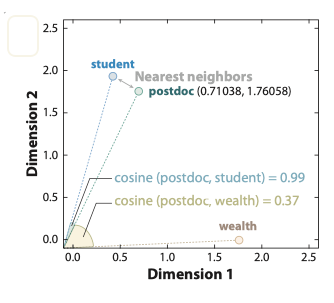
\includegraphics[width=0.55\linewidth]{images/03-marco-teorico/word_vec} 

}

\caption{Representación de palabras en un plano}\label{fig:embeddingimg}
\end{figure}

De esta manera se tiene que, al generar la representación completa de un espacio semántico, haciendo la búsqueda de una palabra podemos encontrar también aquellas que son cercanas y no limitar la búsqueda al \emph{match} que los modelos anteriormente estudiados sí imponían. Más adelante también veremos que el modelo semántico puede ser expandido y representar mediante un \emph{embedding} oraciones (\emph{sentences}), siendo esto el sustento que permite que al hacer una pregunta o un \emph{query} a un sistema de recuperación de información, este sea capaz de encontrar la respuesta dentro del corpus, ya que la pregunta o \emph{query} se transforma en un \emph{embedding} y luego se determina en el espacio semántico cuál es la oración que más se aproxima y guarda algún tipo de proximidad o relación de distancia vectorial con la pregunta formulada.~

Es importante mencionar que, han sido diversos los algoritmos implementados para crear los \emph{embeddings}, evolucionando para lograr que las representaciones de los textos resulten de mayor provecho y rendimiento. A manera ilustrativa, para comprender una parte del funcionamiento de los \emph{embeddings,} se va a usar el modelo ``\emph{GloVe: Global Vectors for Word Representation}'' (\protect\hyperlink{ref-pennington2014}{Pennington, Socher, y Manning 2014}) en el cual mediante un vector de 100 componentes, siendo cada uno de estos un número real de ocho o más decimales, se logra hacer la representación de una palabra. A continuación se muestran los componentes del vector obtenido para el vocablo \emph{king}, simplificado en este caso a 50 componentes principales:

``0.50451, 0.68607, -0.59517, -0.022801, 0.60046, -0.13498, -0.08813, 0.47377, -0.61798, -0.31012, -0.076666, 1.493, -0.034189, -0.98173, 0.68229, 0.81722, -0.51874, -0.31503, -0.55809, 0.66421, 0.1961, -0.13495, -0.11476, -0.30344, 0.41177, -2.223, -1.0756, -1.0783, -0.34354, 0.33505, 1.9927, -0.04234, -0.64319, 0.71125, 0.49159, 0.16754, 0.34344, -0.25663, -0.8523, 0.1661, 0.40102, 1.1685, -1.0137, -0.21585, -0.15155, 0.78321, -0.91241, -1.6106, -0.64426, -0.51042''

No obstante, ya que estos números dificultan la comprensión intuitiva, con la finalidad de facilitar el análisis, el vector revisado se procede a representarlo gráficamente en la Figura \ref{fig:embking}, mapeando los componentes a una paleta de colores.

\begin{figure}

{\centering 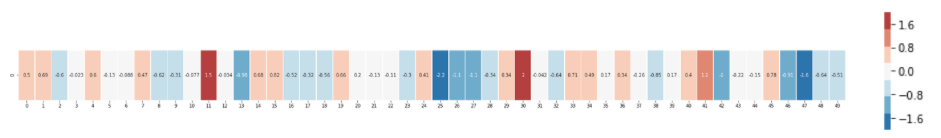
\includegraphics[width=0.95\linewidth]{images/03-marco-teorico/embking} 

}

\caption{Representación de palabra king mediante el modelo GloVe}\label{fig:embking}
\end{figure}

Igualmente, usando el mismo modelo y método de visualización, una representación de las palabras \emph{king} (rey), \emph{man} (hombre) y \emph{woman} (mujer) es la que se observa en la imagen \ref{fig:GloVeEmbedd}.

\begin{figure}

{\centering 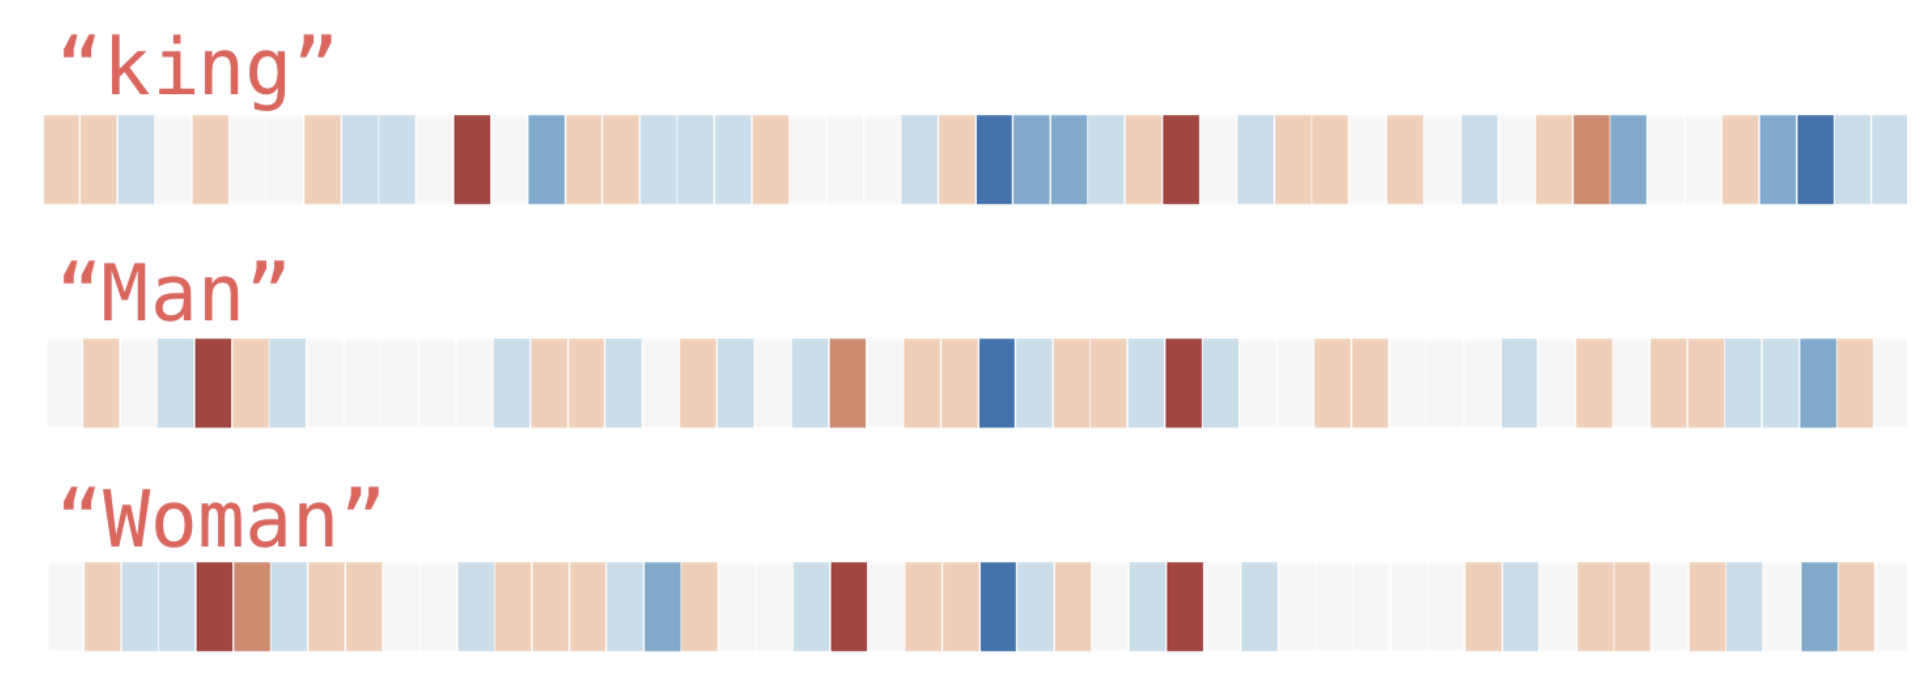
\includegraphics[width=0.95\linewidth]{images/03-marco-teorico/embedding} 

}

\caption{Representación de palabras mediante el modelo GloVe}\label{fig:GloVeEmbedd}
\end{figure}

En tal sentido se tiene que, la representación muestra gráficamente que las palabras \emph{man} y \emph{woman} son más ``parecidas'' visualmente que \emph{king} y \emph{man}, idea que se puede generalizar para entender cómo las distintas palabras que se llevan aun espacio semántico pueden presentar proximidades, similitudes o diferencias, obteniendo de esta forma un significado semántico según la posición relativa que cada una tenga con respecto a la otra en el espacio. El crédito a la visualización que se muestra en \ref{fig:GloVeEmbedd} corresponde al divulgador Jay Alammar (\protect\hyperlink{ref-wordtovec}{Alammar 2023}).

No obstante, en los puntos expuestos aún no se ha explicado cómo se generan los \emph{embeddings}, lo cual es indispensable para entender sus capacidades. Retrotrayéndonos al año 2003, se hizo una investigación en la cual se obtuvo que mediante el entrenamiento de redes neuronales de aprendizaje profundo se logrará modelar la probabilidad y así predecir, las secuencias de palabras dentro de los textos, demostrando la capacidad de estas redes para capturar patrones complejos en datos textuales (\protect\hyperlink{ref-Bengio:2003:NPL:944919.944966}{Bengio et~al. 2003}). Así mismo, también se tiene como otro hito la investigación ``\emph{Semantic Hashing}'' (\protect\hyperlink{ref-salakhutdinov2009}{Salakhutdinov y Hinton 2009}) donde se usaron redes neuronales para transformar datos de alta dimensionalidad en representaciones binarias de baja dimensionalidad. Esa investigación también añadió como un aporte el que se empezarán a usar técnicas de aprendizaje no supervisado para entrenar las redes, deshaciéndose de los cuellos de botella que previamente introducían los procesos de etiquetado, necesarios en métodos supervisados.

Otro punto a resaltar fue lo que significó la ampliación de capacidades de computo en sistemas distribuidos compuestos por tarjetas gráficas (\emph{Graphics Processing Unit} - GPU) a inicios de 2010, ya que este tipo de procesadores facilitan los cálculos de las redes neuronales, con lo cual se empezó a incrementarse el entrenamiento y uso de estas redes para ese momento. También fue para aquel entonces, cuando se publica la investigación \emph{``Word2Vec: Efficient Estimation of Word Representations in Vector Space}'' (\protect\hyperlink{ref-mikolov2013}{Mikolov, Chen, et~al. 2013}) que implementa la técnica \emph{Skip-gram} y \emph{Continuous Bag of Words (CBOW)} que permitieron a las redes el aprendizaje de representaciones semánticas de palabras a partir de grandes volúmenes de texto. \emph{Word2Vec} no solo demostró ser eficiente computacionalmente, sino que también producía \emph{embeddings} que capturaban relaciones semánticas y sintácticas transformando cómo se abordaban las tareas de NLP y las aplicaciones de recuperación de información.

Como consecuencia, una vez que se empezó a tener un método para capturar la semántica de las palabras, debió seguir el paso de lograr representar el sentido semántico de frases (\emph{sentences} en inglés) y expresiones más complejas. Lo anterior se logró con la investigación ``\emph{Distributed Representations of Words and Phrases and their Compositionality}'' (2013) (\protect\hyperlink{ref-mikolov2013a}{Mikolov, Sutskever, et~al. 2013}) donde se hicieron representaciones vectoriales distribuidas para frases, mejorando la capacidad de capturar significados contextuales y relaciones sintácticas en un nivel más alto, lo cual resultó crucial para mejorar los sistemas de recuperación de información y también para la traducción automática.

Por otra parte, la investigación \emph{GloVe} (\protect\hyperlink{ref-pennington2014}{Pennington, Socher, y Manning 2014}), usada en un punto previo para hacer la representación gráfica de tres palabras, también motivó grandes avances al superar limitaciones que presentaban investigaciones anteriores al permitir generar analogías del tipo: (vector de \emph{embedding} para la palabra ``rey'') (menos -) (vector de \emph{embedding} para la palabra ``hombre'') (más +) (\emph{embedding} para la palabra ``mujer''), (es igual=) o muy aproximado en el espacio semántico, al (vector de \emph{embedding} de la palabra ``reina'') o simplificado como ``rey-hombre+mujer = reina''.

Igualmente, con esa investigación se intensificó el uso de esos modelos en tareas de clasificación de texto, como las revisadas en \ref{nlproc},``Procesamiento del Lenguaje Natural'', ya que las redes neuronales empezaron a entrenarse con representaciones de vectores de gran densidad que contenían las palabras, el POS y el etiquetado de las dependencias, conteniendo cada vector 200 componentes y de esta manera se alcanzaron mejores indicadores de desempeño en el etiquetado (\protect\hyperlink{ref-chen2014}{Chen y Manning 2014a}). Cabe destacar que el trabajo citado fue el que dio soporte a la librería revisada anteriormente de nombre ``coreNLP'' de la Universidad de Stanford.

\hypertarget{trans}{%
\subsection{\texorpdfstring{Arquitectura de Redes Neuronales \emph{Transformers}}{Arquitectura de Redes Neuronales Transformers}}\label{trans}}

En el año 2017 se publica ``\emph{Attention Is All You Need}'' (\protect\hyperlink{ref-vaswani2017}{Vaswani et~al. 2017}) el cual fue una investigación donde se introdujo una nueva arquitectura de redes neuronales que eliminó ciertas limitaciones que venían presentando los modelos de redes recurrentes y las convolucionales en poder trabajar con largas cadenas de texto. La solución introdujo los llamados ``mecanismos de atención'' \footnote{Los mecanismos de atención permiten al modelo asignar ponderaciones dinámicas a diferentes partes de la entrada, lo que resulta en una comprensión más profunda y contextualizada del texto.} que abrieron el camino para la creación de nuevos modelos de lenguaje como BERT (\protect\hyperlink{ref-devlin2018}{Devlin et~al. 2018}) que capturaban la riqueza de significados y las relaciones complejas del lenguaje mejorando la comprensión de textos, traducción automática y la generación de texto.

Igualmente destacó el trabajo ``\emph{RoBERTa: A Robustly Optimized BERT Pretraining Approach}'' (\protect\hyperlink{ref-liu2019}{Liu et~al. 2019}) en el que se optimizó el entrenamiento preexistente de \emph{BERT} al desvincular la tarea de pre-entrenamiento del tamaño de la cantidad de ejemplos de entrenamiento (\emph{batch size}) y la duración del entrenamiento. Al escalar el tamaño del lote y la cantidad de datos, \emph{RoBERTa} mejoró la comprensión del modelo sobre el lenguaje, logrando una capacidad de generalización excepcional.

Como consecuencia, estos métodos que venían innovando e incrementando las capacidades, por otra parte también hacían que el tamaño de los conjuntos de datos usados para el entrenamiento fuese creciendo exponencialmente, como se analizará en la sección \ref{LLM}, ``Largos Modelos de Lenguaje''.

En este mismo orden de ideas se tiene que, otro modelo basado en la arquitectura \emph{Transformers} que es necesario referir, ya que a un componente del SCSU le da soporte, es el que se publicó bajo el título ``\emph{Sentence-BERT: Sentence Embedding}s'' (\protect\hyperlink{ref-reimers2019a}{Reimers y Gurevych 2019}) que a diferencia de los modelos anteriormente expuestos, que trabajaban con la codificación de palabras, en él se logra la codificación de oraciones usando una variante de \emph{BERT} (\protect\hyperlink{ref-devlin2018}{Devlin et~al. 2018}) permitiendo entender la similitud semántica entre pares de estas.

Sin embargo, un punto que fue necesario resolver para masificar la adopción de estos modelos era lograr contar con representaciones de \emph{embeddings} para distintos idiomas, ya que inicialmente solo estaban entrenados con textos en idioma inglés impidiendo que fueran de utilidad para otras lenguas. En este sentido, una de las investigaciones que permitió avanzar hacia modelos multilingües fue ``\emph{Making Monolingual Sentence Embeddings Multilingual}'' (\protect\hyperlink{ref-reimers2020}{Reimers y Gurevych 2020}), usando la técnica ``\emph{Knowledge Distillation}'', la cual permitió que en lugar de entrenar modelos para cada idioma, solo se utilice un único modelo de referencia monolingüe para guiar el entrenamiento de modelos en múltiples idiomas, basándose en la idea de que ``una frase traducida debe situarse en el mismo lugar del espacio vectorial-semántico que la frase original'' (\protect\hyperlink{ref-reimers2020}{Reimers y Gurevych 2020}).

En complemento a estas investigaciones, también se tiene a ``\emph{BETO: Spanish BERT}'' (\protect\hyperlink{ref-CaneteCFP2020}{Cañete et~al. 2020}), que teniendo como sustento BERT, fue un modelo entrenado por el Departamento de Ciencias de la Computación Universidad de Chile, disponible en el enlace \url{https://github.com/dccuchile/beto}, al cual se considera como perteneciente el estado del arte para el idioma español, alcanzando una precisión del 98,97\% en tareas como el POS. También se aprovecha de indicar que este modelo igualmente se insertó en la implementación del SCSU.

Otro aspecto que es necesario señalar es que todas las investigaciones citadas se hicieron de dominio público y en muchos casos también se colocó a disposición de la comunidad científica los propios modelos preentrenados y los conjuntos de datos del entrenamiento, lo cual conllevó a que se lograra la reproducibilidad de los mismos, beneficiando a la comunidad científica y a los desarrolladores.

En caso de resultar de interés, para obtener información sobre los modelos de \emph{embeddings} que presentan una elevada precisión y son de alta demanda por la comunidad \emph{open source}, siendo parte del estado del arte, se tienen herramientas como el ``\emph{MTEB: Massive Text Embedding Benchmark}'' (\protect\hyperlink{ref-muennighoff2022}{Muennighoff et~al. 2022}), al que se puede acceder en el enlace \url{https://huggingface.co/spaces/mteb/leaderboard}, donde muestran métricas de 140 modelos preentrenados en el área del lenguaje disponibles para el uso público.

\hypertarget{LLM}{%
\subsection{Largos Modelos de Lenguaje}\label{LLM}}

Con la aparición de la arquitectura \emph{Tranformers} se abrió el camino para la aparición de los Largos Modelos de Lenguaje \emph{(Large Language Models -LLM´s)}. En principio pudiese parecer estar fuera del alcance de este trabajo exponer estos modelos, pero el estado del arte de los sistemas de recuperación de información se intersecta con ellos y no resultan ajenos a trabajos futuros que puedan suceder a esta investigación.

Como se pudo ver en la sección \ref{embed}, ``\emph{Embeddings''}, la tendencia ha sido ir incrementando la cantidad de datos con que se entrenan estos modelos así como también el número de parámetros que conforman al propio modelo. En la Figura \ref{fig:llm}, vemos las variaciones increméntales que se han dado desde la publicación del modelo basado en los \emph{Transformers} en el año 2017.

\begin{figure}

{\centering 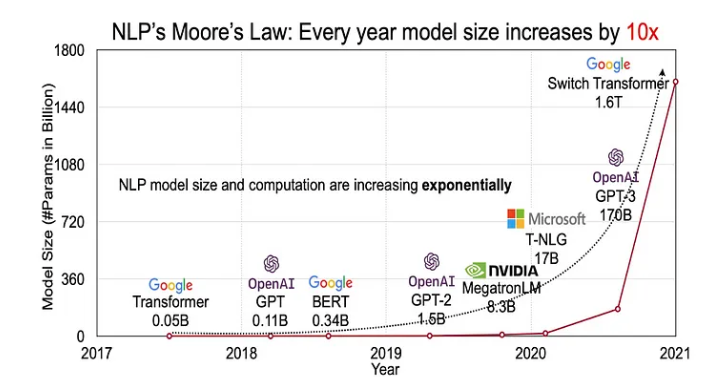
\includegraphics[width=0.85\linewidth]{images/03-marco-teorico/llms} 

}

\caption{Evolución en la cantidad de parámetros en los LLM}\label{fig:llm}
\end{figure}

El crédito a la visualización \ref{fig:llm} corresponde a Harishdatala (\protect\hyperlink{ref-llmsize}{Harishdatala 2023}). En general, los largos modelos de lenguaje son entrenados con enormes corpus de textos recopilados de foros de internet, de páginas web, de libros digitalizados y de un basto cúmulo de textos que también pueden incluir datos sintéticos.

De esta manera, sin entrar en mayores consideraciones sobre este crecimiento y los costos asociados, tanto monetarios, ambientales y de recursos computacionales, que imposibilitan a instituciones educativas, a empresas de mediano tamaño o a investigadores independientes, poder acceder a los sistemas de computadores necesarios para entrenar modelos de estas características, resulta significativo que a finales del año 2022 a uno de los modelos llamado ``\emph{Generative Pre-trained Transformer 3}'' de la empresa OpenAI, del cual no se dispone mayor documentación sobre su arquitectura ni precisión sobre el método de entrenamiento, le es realizado un proceso de ``\emph{fine tunning}'' que es un ajuste a los parámetros mediante un reentrenamiento y así se crea lo que hoy se conoce comercialmente como ChatGPT 3.5, introduciendo mediante una interfaz de usuario la funcionalidad de que se pueda interactuar con el modelo simulando una conversación, sorprendiendo por la capacidad de lograr emitir respuestas sobre una gran diversidad de temas de una manera fluida.

En complemento de lo anterior se tiene que, representando la interacción humano - LLM mediante una analogía con los SRI, lo que se aprecia es a un usuario haciendo un \emph{query} ante un enorme corpus que excede y se organiza de una forma distinta a lo que se había revisado en \ref{SRI}, ``Sistemas de Recuperación de Información'', donde se tenía una base de datos con documentos indexados. Ahora son distintos, tanto el proceso de interacción, como la representación de la información, ya que cada vez que se solicita un \emph{query}, lo primera diferencia que se tiene es que, puede ser expresado en lenguaje natural y la segunda, es que no debe ser una condición que se de algún \emph{match} con una palabra que conforma el índice invertido. En realidad el texto de la consulta es transformado en un \emph{embedding,} que posteriormente activa capas de la red neuronal, conformadas las mismas por los parámetros del modelo y así de esta forma, mediante un proceso estocástico, el LLM va prediciendo palabra a palabra, conformando una respuesta a lo que fue el \emph{query} inicial. Lo anterior puede cubrir la necesidad de información requerida con respuestas que estén acorde a lo esperado, siendo novedosas, fidedignas, o no tanto, a la realidad. Sin embargo, no se debe olvidar que la calidad del texto de la respuesta que produzca el LLM, dependerá de aspectos que traspasan lo computacional y se asocian un tanto más a las previsiones que se hayan tomado, por parte de quienes entrenan el modelo, para mitigar sesgos contenidos en los textos o entradas de datos incorrectas en la fase de entrenamiento del mismo.

Por otra parte, es indispensable resaltar como un hecho muy importante en el campo de los LLM´s que en el año 2023 algunas compañías e institutos de investigación privados, empezaron a liberar de licencias de uso ciertos modelos, con distintos pesos y versiones para la comunidad \emph{open source}, como lo es el modelo Falcon (\protect\hyperlink{ref-penedo2023}{Penedo et~al. 2023}) o el modelo OpenLlama2 (\protect\hyperlink{ref-touvron2023}{Touvron et~al. 2023}) \footnote{la compañía que entrenó el modelo y lo liberó que es Meta indicó que es OpenSource, pero revisiones técnicas hechas a la licencia cuestionan que se pueda considerar que realmente cumpla las especificaciones para que sea considerado plenamente ``open source''. En el enlace \href{https://opensourceconnections.com/blog/2023/07/19/is-llama-2-open-source-no-and-perhaps-we-need-a-new-definition-of-open/}{Is Llama 2 open source?} se encuentra un análisis sobre el tema.}. Lo anterior, en conjunto con las facilidades para el desarrollo que aportan plataformas como \url{huggingface.com} para la implementación de aplicaciones de inteligencia artificial, mediante el almacenamiento de modelos preentrenados, conjuntos de datos para entrenamiento o sobre entrenamiento, así como librerías con \emph{pipelines} de fácil integración mediante API´s unificadas (\protect\hyperlink{ref-wolf2019}{Wolf et~al. 2019}), estos LLM´s dejaron de tener un uso limitado solo para grandes empresas o consorcios tecnológicos y para la fecha es viable que corran en computadoras con capacidades limitadas, mediante la aplicación de procesos como el \emph{quantized}, que se presenta en la investigación (\protect\hyperlink{ref-dettmers2023}{Dettmers et~al. 2023}), que por ejemplo permite que un modelo de lenguaje que inicialmente necesita unos 16 GB de memoria RAM en GPU para ser desplegado, pueda disminuir a una cuarta parte, 4 GB, haciendo viable que se pueda desplegar en un computador con menores recursos disponibles.

Para cerrar el tema, la diversidad de modelos preentrenados, con distintas versiones que les ha sido efectuado un proceso de \emph{fine tunning} o cuantizaciones, se puede ver en el enlace (\protect\hyperlink{ref-openllm}{Edward Beeching 2023}) \url{https://huggingface.co/spaces/HuggingFaceH4/open_llm_leaderboard} , donde se encuentra un tablero que muestra los modelos que presentan mayor popularidad, descargas y métricas de evaluación de su comportamiento.

\hypertarget{int}{%
\subsection{Integración}\label{int}}

Al contar con versiones \emph{open source} de estos modelos es posible integrarlos en procesos de recuperación de información, principalmente mediante dos técnicas.

\begin{enumerate}
\def\labelenumi{\arabic{enumi}.}
\item
  \emph{Retrieval Augmented Generation RAG} (\protect\hyperlink{ref-lewis2020}{Lewis et~al. 2020}): esta técnica permite que un LLM que fue entrenado con un determinado corpus, pueda activar la extracción de información desde fuentes externas, como páginas de internet o una bases de datos, complementando la información que inicialmente dispone el modelo, asociada a los datos de entrenamiento. Cabe destacar que, específicamente al hablar de las bases de datos que almacenan \emph{embeddings}, a estas se les denomina \emph{Vector DataBase.} Bien sea que el modelo de lenguaje acuda a una página de internet o a la \emph{Vector Database}, una vez que la información se recupera, el LLM se encarga de procesarla e integrarla en una respuesta que debe tener una estructura compresible y coherente.
\item
  \emph{Fine Tunning} (\protect\hyperlink{ref-lv2023}{Lv et~al. 2023}): con un conjunto de datos etiquetado, generalmente con información de un dominio específico de un volumen mucho menor al que inicialmente fue entrenado un determinado LLM, se puede lograr que el modelo sea sobreentrenado con métodos como el propuesto en la investigación \emph{``Universal Language Model Fine-tuning for Text Classification}'' (\protect\hyperlink{ref-howard2018}{Howard y Ruder 2018}), mejorando notablemente su desempeño en emitir respuestas sobre ese particular dominio en el que se realizó el ajuste.
\end{enumerate}

En resumen, estas técnicas por separado o en paralelo, pueden implementarse para crear sistemas de recuperación de información soportados en un LLM, el cual se pueda adaptar y convertirse en un experto de una precisa área de estudio que indique referencias a los trabajos que conforman un determinado corpus.

\hypertarget{busquedasemantica}{%
\subsection{Búsqueda Semántica}\label{busquedasemantica}}

Es una evolución en la forma en que los motores de búsqueda comprenden y responden a las consultas. A diferencia de la búsqueda tradicional basada en la aparición de palabras clave, la cual se centra en encontrar coincidencias literales entre la consulta y el contenido web, la búsqueda semántica tiene como objetivo comprender el significado contextual de las consultas y ofrecer resultados más relevantes y precisos.

Para ahondar en la comprensión de su significado, se tiene que en lugar de simplemente emparejar palabras clave, la búsqueda semántica utiliza \emph{embeddings} para representar el texto y de una mejor forma se logra comprender la intención que motiva la consulta, lo cual implica que se analiza la relación semántica entre las palabras, interpretando el contexto y comprendiendo el significado subyacente.

En tan sentido, desde un punto de vista relativo a la implementación, se tiene que en las búsquedas semánticas las cadenas de texto de un documento se representan como vectores de tipo \emph{embeddings,} los cuales son almacenados en una base de datos y el sistema de recuperación de información al recibir un \emph{query} transforma el texto en otro \emph{embedding}, lo cual permite determinar el grado de similitud vectorial y así proceder a recuperar los documentos que presenten mayor parecido (\protect\hyperlink{ref-muennighoff2022a}{Muennighoff 2022}).

Es importante destacar de manera muy particular que, el éxito que se obtenga al usar este tipo de búsqueda dependerá en una gran medida de la correcta selección del modelo de aprendiza automático preentrenado que se use para convertir los textos a \emph{embeddings}. Por ejemplo, existen modelos que han sido entrenados para un idioma o para un dominio específico, lo cual hará que un sistema de recuperación de información que sea diseñado para un uso particular, se verá beneficiado si se selecciona un modelo acorde a sus necesidades.

\hypertarget{tendencias-actuales}{%
\subsection{Tendencias Actuales}\label{tendencias-actuales}}

Finalmente, se hace mención a algunos puntos de lo que hoy constituye el estado del arte en los temas que hemos ido revisando a lo largo de este capítulo:

\begin{enumerate}
\def\labelenumi{\arabic{enumi}.}
\item
  Con modelos como BERT se han hecho implementaciones modificadas para hacer el reordenamiento de los resultados obtenidos en un proceso de búsqueda, bien sea mediante las técnicas tradicionales o mediante técnicas de búsqueda semántica(\protect\hyperlink{ref-nogueira2019}{Nogueira y Cho 2019}). Igualmente, con redes neuronales se ha buscado simular el comportamiento humano para jerarquizar los resultados obtenidos en procesos de búsqueda (\protect\hyperlink{ref-pang2017}{Pang et~al. 2017}).
\item
  Se están proponiendo nuevos métodos para evaluar la eficacia en los sistemas de ``preguntas-respuestas'' basados en similaridad semántica, dadas las limitaciones que presentan las métricas tradicionales que no reflejan el desempeño de estos nuevos modelos (\protect\hyperlink{ref-risch2021}{Risch et~al. 2021}).
\item
  Mediante técnicas de aprendizaje profundo se están creando conjuntos de datos sintéticos de dominio público que permitan evaluar el desempeño de los sistemas de recuperación de información, usando como entrada las publicaciones de Wikipedia y creando con estos modelos los \emph{querys}, que permitan medir el grado de precisión que alcanza un determinado sistema (\protect\hyperlink{ref-frej-etal-2020-wikir}{Frej, Schwab, y Chevallet 2020}).
\end{enumerate}

Expuestos los puntos anteriores se culmina el recorrido del marco teórico-referencial que soporta esta investigación.

\hypertarget{mm}{%
\chapter{Marco Metodológico}\label{mm}}

En este capítulo se indican los métodos de trabajo que se usaron para el desarrollo de la investigación y para el desarrollo e implementación del Sistema Complementario Saber UCV.

\hypertarget{mmmetodologia}{%
\section{Método de Trabajo Kanban}\label{mmmetodologia}}

En este método se fomenta la cultura de mejora continua e incremental al identificar cuellos de botella y la limitación del trabajo en curso para aumentar la eficiencia y la productividad. Gracias a su enfoque basado en la colaboración, flexibilidad y respuesta rápida a los cambios, puede considerarse que está dentro de las metodologías ágiles.

En tal perspectiva, mediante la visualización del flujo de trabajo en un tablero, que se aprecia en la Figura \ref{fig:metkanban}, se puede facilitar la gestión del proyecto desde la concepción de una idea hasta su implementación y entrega. En el caso del desarrollo de software, facilita la toma de decisiones informadas y promueve la transparencia al proporcionar una visualización clara de las tareas y actividades involucradas (\protect\hyperlink{ref-stephens2015}{Stephens 2015}).

\begin{figure}

{\centering 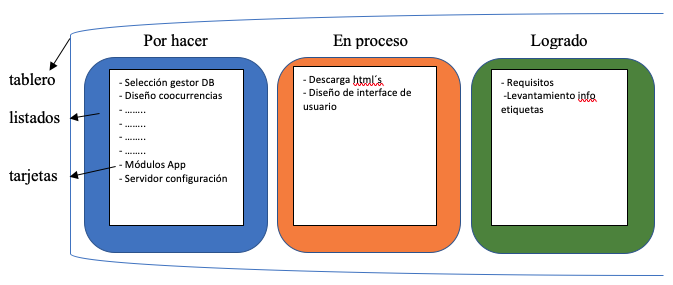
\includegraphics[width=0.7\linewidth]{images/04-metodologia/01_kanban} 

}

\caption{Representación de un tablero según el método Kanban}\label{fig:metkanban}
\end{figure}

Es de resaltar que, durante el desarrollo e implementación del SCSU se necesitaba contar con la flexibilidad que ofrece este método, ya que en él no se tienen que definir roles específicos en el equipo desarrollador, ni tampoco es necesario establecer períodos fijos para alguna fase en particular.

\hypertarget{mmasd}{%
\section{Desarrollo Adaptable de Software}\label{mmasd}}



El ``\emph{Adaptive Software Development ASD''} (\protect\hyperlink{ref-highsmith2000}{Highsmith 2000}) es un método ágil de desarrollo de software que se centra en la adaptabilidad y capacidad para adaptarse a los cambios, proporcionando una retroalimentación temprana y frecuente dando flexibilidad para abordar los desafíos cambiantes del desarrollo de software. A diferencia de los enfoques tradicionales, el ASD reconoce la naturaleza impredecible del desarrollo de software y se adapta continuamente para satisfacer las necesidades del cliente en un entorno dinámico y complejo, haciendo énfasis en el precepto ``entregar el proyecto que se necesita al final, no el proyecto que se pidió al principio''.

\hypertarget{caracteruxedsticas}{%
\subsection{Características}\label{caracteruxedsticas}}

\textbf{Colaboración y Comunicación Constante:} fomenta la colaboración cercana entre los equipos de desarrollo y los \emph{stakeholders}. La comunicación constante permite una comprensión profunda de los requisitos del cliente y facilita ajustes rápidos según las necesidades cambiantes.

\textbf{Iteraciones Incrementales:} divide el proyecto en iteraciones cortas y manejables. Cada iteración produce un incremento funcional del software, lo que permite obtener retroalimentación temprana que permite corregir errores y ajustar el rumbo del proyecto antes de que los problemas se vuelvan críticos.

\textbf{Flexibilidad y Adaptabilidad:} reconoce que los requisitos del proyecto pueden cambiar con el tiempo. Por lo tanto, se adapta fácilmente a los cambios permitiendo una rápida reevaluación y ajuste de las estrategias y metas del proyecto asegurando que el producto final esté alineado de manera óptima con las necesidades y expectativas del cliente, incluso en un entorno de desarrollo volátil.

\hypertarget{ciclos-de-desarrollo}{%
\subsection{Ciclos de Desarrollo}\label{ciclos-de-desarrollo}}

El desarrollo adaptable de software se basa en un proceso dinámico e iterativo donde cada ciclo contiene las siguientes fases: especular-colaborar-aprender. El proceso se enfoca en el aprendizaje continuo y la colaboración intensiva entre desarrolladores y clientes, fundamental para enfrentar las cambiantes dinámicas empresariales. Es relevante destacar que en algunas circunstancias los ciclos pueden avanzar simultáneamente en ciertas iteraciones, permitiendo así una optimización del tiempo y recursos.

Bajo esta concepción, en cada ciclo se pueden realizar múltiples iteraciones con el objetivo de desarrollar exhaustivamente todos los requisitos contemplados.

Es necesario destacar que, estos ciclos representan un enfoque metodológico que asegura la coherencia y calidad del desarrollo del sistema. A través de la especulación, la colaboración y el aprendizaje continuo, se logra un refinamiento progresivo de las funcionalidades del sistema, garantizando así su robustez y adaptabilidad a las demandas del entorno. Este enfoque iterativo y colaborativo constituye una práctica fundamental en el proceso de desarrollo, facilitando la identificación temprana de posibles desafíos y fomentando la innovación constante en cada etapa del ciclo.

\begin{figure}

{\centering 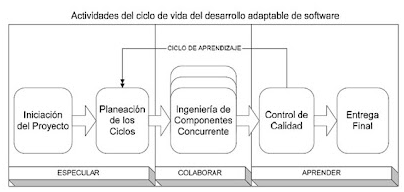
\includegraphics[width=0.6\linewidth]{images/04-metodologia/02_ciclo} 

}

\caption{Ciclo ASD}\label{fig:metdas}
\end{figure}

\hypertarget{especulaciuxf3n}{%
\subsubsection{\texorpdfstring{\textbf{Especulación}}{Especulación}}\label{especulaciuxf3n}}

Este componente ofrece un espacio para la exploración y la comprensión de la incertidumbre. Permite desviarse del plan inicial sin temor, transformando los errores en oportunidades de aprendizaje. Es necesario aceptar que no se sabe todo, y así impulsar la disposición para aprender y experimentar.

\hypertarget{colaboraciuxf3n}{%
\subsubsection{\texorpdfstring{\textbf{Colaboración}}{Colaboración}}\label{colaboraciuxf3n}}

Las aplicaciones complejas requieren la recopilación y el análisis de grandes volúmenes de información y ejecución de tareas. Este proceso es inmanejable para un individuo. En entornos dinámicos, donde fluyen grandes cantidades de datos, es esencial la colaboración ya que un solo individuo o un pequeño grupo, no puede abarcar todo el conocimiento necesario.

\hypertarget{aprendizaje}{%
\subsubsection{\texorpdfstring{\textbf{Aprendizaje}}{Aprendizaje}}\label{aprendizaje}}

La evaluación continua del conocimiento a través de retroalimentaciones y reuniones grupales al final de cada ciclo iterativo es esencial, lo cual difiere de la evaluación al final del proyecto. Evaluar constantemente permite enfrentar y resolver de manera efectiva los cambios constantes del proyecto y su adaptación a entornos dinámicos y complejos.

\hypertarget{desarrollo}{%
\chapter{Desarrollo de la Solución}\label{desarrollo}}

\hypertarget{desarollodescripcion}{%
\section{Descripción General de la Solución}\label{desarollodescripcion}}

Se implementa un sistema de recuperación de información sobre un corpus de documentos de tesis de grado y trabajos de grado que originalmente se encuentran alojados en el repositorio digital Saber UCV . Utilizando técnicas de extracción de datos de archivos html, desde la ficha de cada investigación se obtiene: el título, el nombre del autor, palabras clave, fecha de publicación, el resumen y el \emph{enlace} de descarga del documento que la sustenta.

Posteriormente, el sistema descarga el documento referenciado en cada ficha, el cual contiene el texto completo de la investigación, da lectura y clasifica la información sobre el nombre de la facultad, la escuela o postgrado donde fue realizado el trabajo e igualmente extrae el nombre del tutor.

Como consecuencia, todos los datos obtenidos son sometidos a técnicas del estado del arte en el procesamiento del lenguaje natural y la minería de texto para conformar un corpus anotado, un índice invertido y una tabla con los vectores de \emph{embeddings} (\emph{Vector Database}), esenciales para un eficiente manejo de la base de datos.

Adicionalmente, el sistema incluye una aplicación web que permite a los usuarios desde un navegador explorar extensivamente el corpus anotado, realizando consultas de texto y aplicando varios filtros como la selección de la jerarquía, el área académica y el rango de fechas.

Complementariamente, la relevancia de los resultados recuperados se determina mediante una función de ponderación y los documentos se presentan de manera priorizada para mejorar la experiencia del usuario.

Adicionalmente, el sistema ofrece recomendaciones de documentos que presentan similitud con aquellos que fueron recuperados en el proceso anterior y muestra mapas de conocimiento mediante una herramienta gráfica interactiva de visualización.

Cabe destacar que la solución implementada cuenta con procesos automatizados de actualización para incorporar las nuevas investigaciones que sean añadidas al repositorio Saber UCV.

Finalmente, el sistema se soporta en un sistema distribuido conformado por contenedores que son gestionados por un orquestador con la arquitectura ``modelo-vista-controlador''.

\hypertarget{desarrolloarquitectura}{%
\section{Arquitectura de la Solución}\label{desarrolloarquitectura}}

La arquitectura ``modelo-vista-controlador'' se muestra en la Figura \ref{fig:arquitecturamvc} y posteriormente se describe el comportamiento y las interacciones de los componentes.

\begin{figure}

{\centering 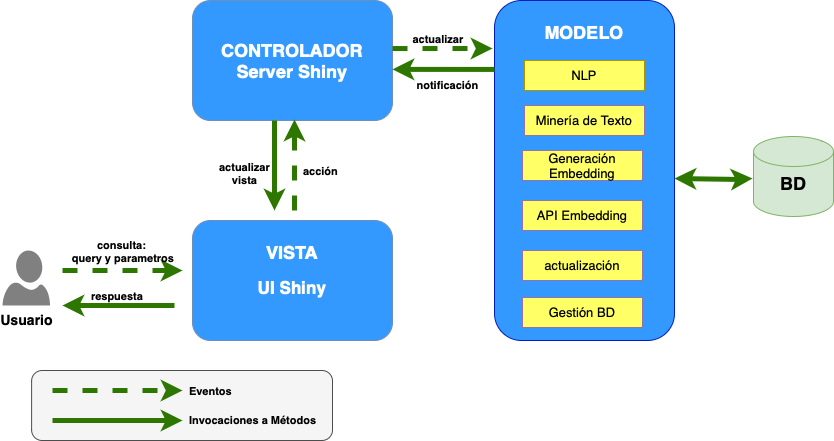
\includegraphics[width=0.9\linewidth]{images/05-desarrollo/MVC9} 

}

\caption{Modelo de Arquitectura MVC}\label{fig:arquitecturamvc}
\end{figure}

\hypertarget{modelo}{%
\subsection{\texorpdfstring{\textbf{Modelo}}{Modelo}}\label{modelo}}

El modelo\emph{,} en el contexto de esta propuesta, es la parte del sistema que se ocupa de la obtención, manipulación y gestión de los datos. Esto incluye la descarga de la información, la clasificación, el procesamiento del lenguaje natural, la minería de texto y la creación del índice invertido. Esta parte del sistema también incluye la lógica para generar los \emph{embeddings} y manejar el corpus anotado. En la implementación del sistema el manejador de base de datos que se usa es PostgreSQL.

En complemento a lo anterior, al modelo igualmente le corresponde realizar las tareas de actualizar el corpus periódicamente y las recomendaciones de documentos a medida que se agreguen nuevos textos en Saber UCV. En \ref{desarrollociclos4}, el tercer ciclo de desarrollo se expondrán con detalle los componentes del modelo y a continuación se enumeran los principales procesos que él sustenta:

\begin{enumerate}
\def\labelenumi{\arabic{enumi}.}
\item
  \textbf{Creación del Índice Invertido:}

  \begin{itemize}
  \item
    Organizar los términos y sus ubicaciones en los documentos para permitir búsquedas eficientes.
  \item
    Asociar cada término con la lista de documentos en los que aparece.
  \end{itemize}
\item
  \textbf{Procesamiento de Texto:}

  \begin{itemize}
  \item
    Tokenización: dividir el texto en palabras o frases significativas.
  \item
    Lematización: reducir las palabras a su forma base para un análisis más preciso.
  \item
    POS: etiquetado de partes del discurso.
  \end{itemize}
\item
  \textbf{Minería de Texto:}

  \begin{itemize}
  \tightlist
  \item
    Análisis de frecuencia: determinar la frecuencia de ocurrencia de palabras o frases.
  \end{itemize}
\item
  \textbf{Generación de Embeddings:}

  \begin{itemize}
  \item
    Utilización de un modelo preentrenado para convertir palabras o frases en vectores numéricos.
  \item
    Convertir en vectores las palabras que componen el \emph{query} para realizar comparaciones semánticas y determinar similitudes entre palabras o documentos.
  \end{itemize}
\item
  \textbf{Gestión de la Base de Datos:}

  \begin{itemize}
  \item
    Almacenar y recuperar datos estructurados para su posterior consulta.
  \item
    Actualizar el corpus con nuevos datos.
  \end{itemize}
\item
  \textbf{Cálculo de Relevancia:}

  \begin{itemize}
  \item
    Aplicar algoritmos para calcular la relevancia de los documentos en función de las consultas del usuario y de los parámetros establecidos con anterioridad.
  \item
    Ordenar los resultados en función de su relevancia para presentar los documentos más relevantes primero.
  \end{itemize}
\item
  \textbf{Actualización de datos:}

  \begin{itemize}
  \item
    Los procesos mencionados previamente son ejecutados y/o actualizados periódicamente.
  \item
    Se realiza la validación de la integridad de datos para asegurar que los nuevos datos se integren correctamente sin errores o inconsistencias, eliminando posibles duplicados o valores incorrectos.
  \end{itemize}
\end{enumerate}

\hypertarget{vista}{%
\subsection{\texorpdfstring{\textbf{Vista}}{Vista}}\label{vista}}

La vista se implementa mediante el \emph{framework} Shiny (\protect\hyperlink{ref-shiny}{Chang et~al. 2023}) \footnote{El framework Shiny incluye dos componentes principales. El primero es la ui (interfaz de Usuario), que corresponde a la ``Vista''. El otro componente es el ``server'' que en la representación actual es el controlador.} que permite crear aplicaciones web interactivas y tiene un componente de ``user inferface (ui)'' donde el usuario interactúa al introducir el texto con el que se hará la búsqueda y aplica los siguientes filtros: jerarquía, área académica nivel 1 (facultad), área académica nivel 2 (escuela o postgrado) y rango de fechas. Posterior a la definición de los atributos del \emph{query}, se desencadenan acciones que son enviadas al controlador y al recibir la respuesta la vista se actualiza y muestra las tablas con los resultados de la búsqueda, las representaciones visuales como el mapas de conocimiento y las recomendaciones de documentos similares.

\hypertarget{controlador}{%
\subsection{\texorpdfstring{\textbf{Controlador}}{Controlador}}\label{controlador}}

El controlador se implementa mediante el \emph{framework} Shiny que tiene un componente denominado ``server'' que es el responsable de manejar las interacciones del usuario, gestionar las consultas de texto y aplicar los filtros seleccionados. También se encarga de orquestar las operaciones entre el modelo y la vista, asegurando que los datos se presenten correctamente y que las consultas se procesen de manera eficiente. Desde el \emph{controlador} se hace el llamado al componente del modelo donde se encuentra la API para generar el \emph{embedding} del \emph{query} y determinar la relevancia de los documentos recuperados. El controlador aplica el re ordenamiento para mostrar en orden los resultados más relevantes. En él se conforma la estructura para representar el mapas de conocimiento con datos obtenidos del \emph{modelo}.

\hypertarget{desarrollociclos}{%
\section{Ciclos de Desarrollo}\label{desarrollociclos}}

Los Ciclos de Desarrollo constituyen fases críticas del proceso donde se conciben, diseñan y perfeccionan las funcionalidades del sistema. Cada uno de estos ciclos está estructurado en tres etapas fundamentales: la etapa de especulación, donde se plantean las ideas y se exploran posibles soluciones; la etapa de colaboración, donde se trabaja en equipo para implementar estas ideas y se evalúan los resultados; y la etapa de aprendizaje, donde se analizan las experiencias pasadas y se ajustan las estrategias para futuras iteraciones.

Para el desarrollo del SCSU se hizo un proceso iterativo donde en cada ciclo se abordó cada una de las fases descritas y así incrementalmente se fueron añadiendo funcionalidades al sistema.

La literatura en este tema siempre especifica a un cliente del que hay que obtener retroalimentación temprana para así adaptar el producto a medida que evoluciona. Esto fue lo que se hizo en reuniones continuas en la materia \emph{Tópicos Especiales en Sistemas de Información y Gerencia} que representó a la unidad requirente (cliente) y así se fueron evaluando los requisitos y se formularon las correspondientes hipótesis, se observó y se midió el desempeño, por ejemplo, en los modelos de aprendizaje automático preentrenados, usados para el procesamiento de los textos.

\newpage

\hypertarget{desarrollociclos1}{%
\subsection{Ciclo - Conformación del Conjunto de Datos}\label{desarrollociclos1}}

En este ciclo es donde se ejecutaron las tareas que permitieron conformar el conjunto de datos acorde a lo planteado en \ref{objeespe}, ``Objetivo Específico - 1''.

\hypertarget{scrapeo}{%
\subsubsection{Iteración- ``Extracción de Datos Web Saber UCV''}\label{scrapeo}}

\textbf{Especulación}

El repositorio Saber UCV en la sección ``Comunidades-Tesis'' aloja las cantidades de trabajos por nivel académico que se muestran en el Cuadro \ref{tab:cantidadesteg} :

\global\setlength{\Oldarrayrulewidth}{\arrayrulewidth}

\global\setlength{\Oldtabcolsep}{\tabcolsep}

\setlength{\tabcolsep}{0pt}

\renewcommand*{\arraystretch}{1.5}



\providecommand{\ascline}[3]{\noalign{\global\arrayrulewidth #1}\arrayrulecolor[HTML]{#2}\cline{#3}}

\begin{longtable}[c]{|p{1.06in}|p{0.78in}|p{1.01in}|p{1.15in}}

\caption{Cantidades\ de\ Trabajos\ por\ Categoría}\label{tab:cantidadesteg}\\

\ascline{1.5pt}{666666}{1-4}

\multicolumn{1}{>{\raggedleft}m{\dimexpr 1.06in+0\tabcolsep}}{\textcolor[HTML]{000000}{\fontsize{11}{11}\selectfont{\global\setmainfont{Helvetica}{\textbf{Pregrado}}}}} & \multicolumn{1}{>{\raggedleft}m{\dimexpr 0.78in+0\tabcolsep}}{\textcolor[HTML]{000000}{\fontsize{11}{11}\selectfont{\global\setmainfont{Helvetica}{\textbf{Otras}}}}} & \multicolumn{1}{>{\raggedleft}m{\dimexpr 1.01in+0\tabcolsep}}{\textcolor[HTML]{000000}{\fontsize{11}{11}\selectfont{\global\setmainfont{Helvetica}{\textbf{Maestría}}}}} & \multicolumn{1}{>{\raggedleft}m{\dimexpr 1.15in+0\tabcolsep}}{\textcolor[HTML]{000000}{\fontsize{11}{11}\selectfont{\global\setmainfont{Helvetica}{\textbf{Doctorado}}}}} \\

\ascline{1.5pt}{666666}{1-4}\endfirsthead \caption[]{Cantidades\ de\ Trabajos\ por\ Categoría}\label{tab:cantidadesteg}\\

\ascline{1.5pt}{666666}{1-4}

\multicolumn{1}{>{\raggedleft}m{\dimexpr 1.06in+0\tabcolsep}}{\textcolor[HTML]{000000}{\fontsize{11}{11}\selectfont{\global\setmainfont{Helvetica}{\textbf{Pregrado}}}}} & \multicolumn{1}{>{\raggedleft}m{\dimexpr 0.78in+0\tabcolsep}}{\textcolor[HTML]{000000}{\fontsize{11}{11}\selectfont{\global\setmainfont{Helvetica}{\textbf{Otras}}}}} & \multicolumn{1}{>{\raggedleft}m{\dimexpr 1.01in+0\tabcolsep}}{\textcolor[HTML]{000000}{\fontsize{11}{11}\selectfont{\global\setmainfont{Helvetica}{\textbf{Maestría}}}}} & \multicolumn{1}{>{\raggedleft}m{\dimexpr 1.15in+0\tabcolsep}}{\textcolor[HTML]{000000}{\fontsize{11}{11}\selectfont{\global\setmainfont{Helvetica}{\textbf{Doctorado}}}}} \\

\ascline{1.5pt}{666666}{1-4}\endhead



\multicolumn{4}{>{\raggedleft}m{\dimexpr 3.99in+6\tabcolsep}}{\textcolor[HTML]{000000}{\fontsize{11}{11}\selectfont{\global\setmainfont{Helvetica}{cifras\ de\ Saber.UCV\ a\ la\ fecha\ 15/10/2023}}}} \\

\ascline{0.75pt}{666666}{1-4}\endfoot



\multicolumn{1}{>{\raggedleft}m{\dimexpr 1.06in+0\tabcolsep}}{\textcolor[HTML]{000000}{\fontsize{11}{11}\selectfont{\global\setmainfont{Helvetica}{8.305}}}} & \multicolumn{1}{>{\raggedleft}m{\dimexpr 0.78in+0\tabcolsep}}{\textcolor[HTML]{000000}{\fontsize{11}{11}\selectfont{\global\setmainfont{Helvetica}{1.477}}}} & \multicolumn{1}{>{\raggedleft}m{\dimexpr 1.01in+0\tabcolsep}}{\textcolor[HTML]{000000}{\fontsize{11}{11}\selectfont{\global\setmainfont{Helvetica}{743}}}} & \multicolumn{1}{>{\raggedleft}m{\dimexpr 1.15in+0\tabcolsep}}{\textcolor[HTML]{000000}{\fontsize{11}{11}\selectfont{\global\setmainfont{Helvetica}{318}}}} \\

\ascline{1.5pt}{666666}{1-4}



\end{longtable}



\arrayrulecolor[HTML]{000000}

\global\setlength{\arrayrulewidth}{\Oldarrayrulewidth}

\global\setlength{\tabcolsep}{\Oldtabcolsep}

\renewcommand*{\arraystretch}{1}

En la minería de datos con la extracción de datos web es posible ``recolectar, procesar, analizar y extraer útiles conocimientos a partir de los datos disponibles'' (\protect\hyperlink{ref-aggarwal2018}{Aggarwal 2018b}). Por esto se planteó replicar en un conjunto de datos alojado localmente la información contenida en el repositorio Saber UCV que asciende a una cantidad de 10.843 investigaciones, incluyendo los siguientes campos: categoría (pregrado, otros, maestría, doctorado), título, autor, fecha de publicación, palabras clave, enlacede descarga \footnote{este \emph{enlace} correponde a el documento escrito del trabajo de grado o tesis que se encuentra alojado en word o pdf.} y resumen. Al obtener esta información se puede dar inicio a la conformación del corpus.

\textbf{Colaboración}

En esta etapa se realizaron dos procesos de extracción de datos web usando el lenguaje de programación R version 4.3.2 (2023-10-31) (\protect\hyperlink{ref-R}{R Core Team 2023}).

\begin{enumerate}
\def\labelenumi{\arabic{enumi}.}
\item
  El primero fue encontrar los enlaces de cada trabajo alojado en el repositorio Saber UCV. Usando la extensión \emph{SelectorGadget} (\protect\hyperlink{0}{https://selectorgadget.com/}) del navegador \emph{Google Chrome} se puede obtener mediante un clic en un elemento de la página la etiqueta css asociada al nodo que se desea extraer. En este caso al visitar la página ``\protect\hyperlink{0}{http://saber.ucv.ve/handle/10872/1957/browse}'', se identificó la etiqueta \texttt{evenRowOddCol}, ver Figura \ref{fig:nodosurl}, que identifica a los nodos dentro de la página que tienen los enlaces \texttt{href} a las fichas de cada investigación.

  Posteriormente, con el paquete rvest (\protect\hyperlink{ref-rvest}{Wickham 2022a}) que permite la descarga de páginas web y la manipulación de nodos XML se pudieron extraer los 10.843 enlaces a visitar.
\end{enumerate}

\begin{figure}

{\centering 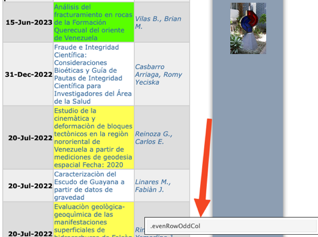
\includegraphics[width=0.5\linewidth]{images/05-desarrollo/1_ciclo/Picture3} 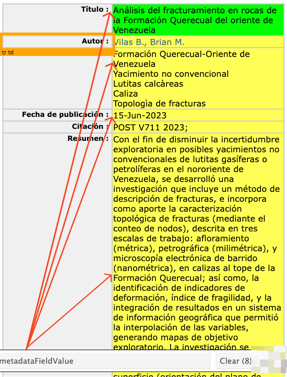
\includegraphics[width=0.5\linewidth]{images/05-desarrollo/1_ciclo/Picture2} 

}

\caption{Etiquetas de nodos url}\label{fig:nodosurl}
\end{figure}

\begin{enumerate}
\def\labelenumi{\arabic{enumi}.}
\setcounter{enumi}{1}
\tightlist
\item
  En una segunda fase, mediante la misma técnica indicada en el punto anterior, se localizó en la ficha de un trabajo la etiqueta css, en este caso la \emph{\texttt{.metadataFieldValue}} que está asociada al nodo que contiene los valores del: título, autor, fecha de publicación, palabras clave, enlace de descarga del documento y el texto del resumen. En la Figura \ref{fig:nodosurl}-b, se aprecia una imagen de la ficha mencionada. Al contar con el listado de enlaces y la identificación de los datos a extraer, se hizo un bucle para visitar cada enlace, se descargó el archivo \texttt{html}, se accedió al nodo, se extrajeron los valores y se fueron almacenando en una estructura de datos.
\end{enumerate}

\textbf{Aprender}

Se enfrentaron las siguientes dificultades y se adoptaron las correspondientes soluciones:

\begin{enumerate}
\def\labelenumi{\arabic{enumi}.}
\item
  Se realizaron varios intentos para la descarga y extracción de los valores. Para la obtención de cada campo, en principio se tomó de referencia la posición fija en que aparecía dentro de la ficha, porque se había asumido que estas tenían la misma estructura para todos los trabajos, sin embargo en algunas aparecían otros valores, p.~ej. el de ``colección'', alterando la posición en que se encuentra el dato a extraer. La solución adoptada fue que primero se localizarán dentro de cada ficha, los títulos de los campos, con esto se generó la lista de los valores posicionales y relativo a estos se extrajeron los valores propuestos.
\item
  Algunos valores de las fechas contenían información parcial faltando el mes y/o el día. Se adoptó un método de imputar el valor ``1'' tanto al mes como al día faltante.
\item
  Adoptar previsiones para caídas del servidor de Saber UCV y resguardar en cada vuelta del bucle la información extraída, para no perder el trabajo de extracción acumulado, en caso de una falla remota o local en el acceso.
\item
  La revisión del conjunto de datos obtenido mostró que existen 861 documentos duplicados, bien sea en el ``título'' o en el texto del ``resumen''. Esto ocurre por la introducción de algún carácter adicional o mínimas alteraciones en el texto. Para descartar estos registros, se aplicó una función de limpieza al texto (convertir a minúscula, remover signos puntuación, etc.). Posteriormente se obtuvieron sendos valores \emph{hash} sobre el título y el resumen y posteriormente se descartaron los \emph{hashes} duplicados. Adicionalmente, se decidió usar el \emph{hash} obtenido del ``título procesado'' como el identificador único de cada documento. La remoción de investigaciones que puedan estar duplicadas es importante efectuarla, ya que al ejecutar los procesos de recuperación de información o la representación de los resultados en mapas de conocimiento, al incluir textos repetidos, creará representaciones distorsionadas. En el Cuadro \ref{tab:cantidadesduplicados}, se muestra la cantidad de los valores detectados por jerarquía.
\end{enumerate}

\global\setlength{\Oldarrayrulewidth}{\arrayrulewidth}

\global\setlength{\Oldtabcolsep}{\tabcolsep}

\setlength{\tabcolsep}{0pt}

\renewcommand*{\arraystretch}{1.5}



\providecommand{\ascline}[3]{\noalign{\global\arrayrulewidth #1}\arrayrulecolor[HTML]{#2}\cline{#3}}

\begin{longtable}[c]{|p{1.07in}|p{1.25in}|p{0.89in}|p{1.21in}}

\caption{Cantidades\ de\ Trabajos\ Duplicados}\label{tab:cantidadesduplicados}\\

\ascline{1.5pt}{666666}{1-4}

\multicolumn{1}{>{\raggedright}m{\dimexpr 1.07in+0\tabcolsep}}{\textcolor[HTML]{000000}{\fontsize{11}{11}\selectfont{\global\setmainfont{Helvetica}{\textbf{Jerarquía}}}}} & \multicolumn{1}{>{\raggedleft}m{\dimexpr 1.25in+0\tabcolsep}}{\textcolor[HTML]{000000}{\fontsize{11}{11}\selectfont{\global\setmainfont{Helvetica}{\textbf{Disponibles}}}}} & \multicolumn{1}{>{\raggedleft}m{\dimexpr 0.89in+0\tabcolsep}}{\textcolor[HTML]{000000}{\fontsize{11}{11}\selectfont{\global\setmainfont{Helvetica}{\textbf{Únicos}}}}} & \multicolumn{1}{>{\raggedleft}m{\dimexpr 1.21in+0\tabcolsep}}{\textcolor[HTML]{000000}{\fontsize{11}{11}\selectfont{\global\setmainfont{Helvetica}{\textbf{Duplicados}}}}} \\

\ascline{1.5pt}{666666}{1-4}\endfirsthead \caption[]{Cantidades\ de\ Trabajos\ Duplicados}\label{tab:cantidadesduplicados}\\

\ascline{1.5pt}{666666}{1-4}

\multicolumn{1}{>{\raggedright}m{\dimexpr 1.07in+0\tabcolsep}}{\textcolor[HTML]{000000}{\fontsize{11}{11}\selectfont{\global\setmainfont{Helvetica}{\textbf{Jerarquía}}}}} & \multicolumn{1}{>{\raggedleft}m{\dimexpr 1.25in+0\tabcolsep}}{\textcolor[HTML]{000000}{\fontsize{11}{11}\selectfont{\global\setmainfont{Helvetica}{\textbf{Disponibles}}}}} & \multicolumn{1}{>{\raggedleft}m{\dimexpr 0.89in+0\tabcolsep}}{\textcolor[HTML]{000000}{\fontsize{11}{11}\selectfont{\global\setmainfont{Helvetica}{\textbf{Únicos}}}}} & \multicolumn{1}{>{\raggedleft}m{\dimexpr 1.21in+0\tabcolsep}}{\textcolor[HTML]{000000}{\fontsize{11}{11}\selectfont{\global\setmainfont{Helvetica}{\textbf{Duplicados}}}}} \\

\ascline{1.5pt}{666666}{1-4}\endhead



\multicolumn{4}{>{\raggedright}m{\dimexpr 4.43in+6\tabcolsep}}{\textcolor[HTML]{000000}{\fontsize{11}{11}\selectfont{\global\setmainfont{Helvetica}{cifras\ de\ Saber.UCV\ a\ la\ fecha\ 15/10/2023}}}} \\

\ascline{0.75pt}{666666}{1-4}\endfoot



\multicolumn{1}{>{\raggedright}m{\dimexpr 1.07in+0\tabcolsep}}{\textcolor[HTML]{000000}{\fontsize{11}{11}\selectfont{\global\setmainfont{Helvetica}{pregrado}}}} & \multicolumn{1}{>{\raggedleft}m{\dimexpr 1.25in+0\tabcolsep}}{\textcolor[HTML]{000000}{\fontsize{11}{11}\selectfont{\global\setmainfont{Helvetica}{8.305}}}} & \multicolumn{1}{>{\raggedleft}m{\dimexpr 0.89in+0\tabcolsep}}{\textcolor[HTML]{000000}{\fontsize{11}{11}\selectfont{\global\setmainfont{Helvetica}{7.634}}}} & \multicolumn{1}{>{\raggedleft}m{\dimexpr 1.21in+0\tabcolsep}}{\textcolor[HTML]{FF0000}{\fontsize{11}{11}\selectfont{\global\setmainfont{Helvetica}{671}}}} \\

\ascline{0.75pt}{666666}{1-4}



\multicolumn{1}{>{\raggedright}m{\dimexpr 1.07in+0\tabcolsep}}{\textcolor[HTML]{000000}{\fontsize{11}{11}\selectfont{\global\setmainfont{Helvetica}{otras}}}} & \multicolumn{1}{>{\raggedleft}m{\dimexpr 1.25in+0\tabcolsep}}{\textcolor[HTML]{000000}{\fontsize{11}{11}\selectfont{\global\setmainfont{Helvetica}{1.477}}}} & \multicolumn{1}{>{\raggedleft}m{\dimexpr 0.89in+0\tabcolsep}}{\textcolor[HTML]{000000}{\fontsize{11}{11}\selectfont{\global\setmainfont{Helvetica}{1.343}}}} & \multicolumn{1}{>{\raggedleft}m{\dimexpr 1.21in+0\tabcolsep}}{\textcolor[HTML]{FF0000}{\fontsize{11}{11}\selectfont{\global\setmainfont{Helvetica}{134}}}} \\

\ascline{0.75pt}{666666}{1-4}



\multicolumn{1}{>{\raggedright}m{\dimexpr 1.07in+0\tabcolsep}}{\textcolor[HTML]{000000}{\fontsize{11}{11}\selectfont{\global\setmainfont{Helvetica}{maestría}}}} & \multicolumn{1}{>{\raggedleft}m{\dimexpr 1.25in+0\tabcolsep}}{\textcolor[HTML]{000000}{\fontsize{11}{11}\selectfont{\global\setmainfont{Helvetica}{743}}}} & \multicolumn{1}{>{\raggedleft}m{\dimexpr 0.89in+0\tabcolsep}}{\textcolor[HTML]{000000}{\fontsize{11}{11}\selectfont{\global\setmainfont{Helvetica}{695}}}} & \multicolumn{1}{>{\raggedleft}m{\dimexpr 1.21in+0\tabcolsep}}{\textcolor[HTML]{FF0000}{\fontsize{11}{11}\selectfont{\global\setmainfont{Helvetica}{48}}}} \\

\ascline{0.75pt}{666666}{1-4}



\multicolumn{1}{>{\raggedright}m{\dimexpr 1.07in+0\tabcolsep}}{\textcolor[HTML]{000000}{\fontsize{11}{11}\selectfont{\global\setmainfont{Helvetica}{doctorado}}}} & \multicolumn{1}{>{\raggedleft}m{\dimexpr 1.25in+0\tabcolsep}}{\textcolor[HTML]{000000}{\fontsize{11}{11}\selectfont{\global\setmainfont{Helvetica}{318}}}} & \multicolumn{1}{>{\raggedleft}m{\dimexpr 0.89in+0\tabcolsep}}{\textcolor[HTML]{000000}{\fontsize{11}{11}\selectfont{\global\setmainfont{Helvetica}{310}}}} & \multicolumn{1}{>{\raggedleft}m{\dimexpr 1.21in+0\tabcolsep}}{\textcolor[HTML]{FF0000}{\fontsize{11}{11}\selectfont{\global\setmainfont{Helvetica}{8}}}} \\

\ascline{1.5pt}{666666}{1-4}



\end{longtable}



\arrayrulecolor[HTML]{000000}

\global\setlength{\arrayrulewidth}{\Oldarrayrulewidth}

\global\setlength{\tabcolsep}{\Oldtabcolsep}

\renewcommand*{\arraystretch}{1}

\hypertarget{labels}{%
\subsubsection{Iteración- Levantamiento de Categorías}\label{labels}}

\textbf{Especulación}



Para poder clasificar cada investigación es necesario contar con las categorías que serán asignadas. Se entiende por ``categoría'' el nombre de la carrera de pregrado o el postgrado, junto con la facultad, que constituyen la oferta de la Universidad Central de Venezuela en educación universitaria.

No obstante, al no encontrarse el listado de categorías disponible en el propio repositorio Saber UCV fue necesario realizar una búsqueda web de esta información, extraerla y estructurarla, para así contar con el conjunto de datos de categorías que permita ejecutar la siguiente iteración, ver \ref{asignacion}, ``Extracción y Clasificación de las Investigaciones''.

\textbf{Colaboración}

Se visitó al sitio web oficial de la Universidad Central de Venezuela para revisar la oferta de pregrados y postgrados. Para los postgrados se encontró para cada categoría (especialización, maestría y doctorado) una página con el listado, p.~ej. \href{http://www.ucv.ve/organizacion/vrac/gerencia-de-investigacion-cientifica-y-humanistica/gerencia-de-estudios-de-postgrado/programas-de-postgrado-ucv/maestria.html}{http://www.ucv.ve/organizacion/maestria.html} \footnote{previendo posibles modificacions en las páginas que contienen los listado de postgrados, se procedió a respaldarlas y forman parte del contenido del repositorio asociado a esta Investigación para garantizar la reproducibilidad de los resultados obtenidos. Para la fecha de redacción de este documento el contenido de los \emph{enlaces} indicados fue modificado}. En la Figura \ref{fig:maestrias}, se aprecian las potenciales etiquetas para las maestrías.

\begin{figure}

{\centering 
\includegraphics[width=0.4\linewidth]{images/05-desarrollo/1_ciclo/maestrias} 

}

\caption{Listado de Maestrías}\label{fig:maestrias}
\end{figure}

Mediante la técnica de recuperación de datos web antes descrita, ver \ref{scrapeo}, ``Extracción de Datos web Saber UCV'', se procedió a extraer el nombre de cada postgrado, añadir el nivel académico y asociar la facultad a la cual está adscrito.

La cantidad de postgrados por nivel académico: doctorado, maestría y especializaciones se muestran en el Cuadro \ref{tab:resultpostgrado}.

\global\setlength{\Oldarrayrulewidth}{\arrayrulewidth}

\global\setlength{\Oldtabcolsep}{\tabcolsep}

\setlength{\tabcolsep}{0pt}

\renewcommand*{\arraystretch}{1.5}



\providecommand{\ascline}[3]{\noalign{\global\arrayrulewidth #1}\arrayrulecolor[HTML]{#2}\cline{#3}}

\begin{longtable}[c]{|p{1.15in}|p{1.01in}|p{1.52in}}

\caption{Cantidades\ de\ Postgrados\ por\ Categoría}\label{tab:resultpostgrado}\\

\ascline{1.5pt}{666666}{1-3}

\multicolumn{1}{>{\raggedleft}m{\dimexpr 1.15in+0\tabcolsep}}{\textcolor[HTML]{000000}{\fontsize{11}{11}\selectfont{\global\setmainfont{Helvetica}{\textbf{Doctorado}}}}} & \multicolumn{1}{>{\raggedleft}m{\dimexpr 1.01in+0\tabcolsep}}{\textcolor[HTML]{000000}{\fontsize{11}{11}\selectfont{\global\setmainfont{Helvetica}{\textbf{Maestría}}}}} & \multicolumn{1}{>{\raggedleft}m{\dimexpr 1.52in+0\tabcolsep}}{\textcolor[HTML]{000000}{\fontsize{11}{11}\selectfont{\global\setmainfont{Helvetica}{\textbf{Especialización}}}}} \\

\ascline{1.5pt}{666666}{1-3}\endfirsthead \caption[]{Cantidades\ de\ Postgrados\ por\ Categoría}\label{tab:resultpostgrado}\\

\ascline{1.5pt}{666666}{1-3}

\multicolumn{1}{>{\raggedleft}m{\dimexpr 1.15in+0\tabcolsep}}{\textcolor[HTML]{000000}{\fontsize{11}{11}\selectfont{\global\setmainfont{Helvetica}{\textbf{Doctorado}}}}} & \multicolumn{1}{>{\raggedleft}m{\dimexpr 1.01in+0\tabcolsep}}{\textcolor[HTML]{000000}{\fontsize{11}{11}\selectfont{\global\setmainfont{Helvetica}{\textbf{Maestría}}}}} & \multicolumn{1}{>{\raggedleft}m{\dimexpr 1.52in+0\tabcolsep}}{\textcolor[HTML]{000000}{\fontsize{11}{11}\selectfont{\global\setmainfont{Helvetica}{\textbf{Especialización}}}}} \\

\ascline{1.5pt}{666666}{1-3}\endhead



\multicolumn{1}{>{\raggedleft}m{\dimexpr 1.15in+0\tabcolsep}}{\textcolor[HTML]{000000}{\fontsize{11}{11}\selectfont{\global\setmainfont{Helvetica}{46}}}} & \multicolumn{1}{>{\raggedleft}m{\dimexpr 1.01in+0\tabcolsep}}{\textcolor[HTML]{000000}{\fontsize{11}{11}\selectfont{\global\setmainfont{Helvetica}{101}}}} & \multicolumn{1}{>{\raggedleft}m{\dimexpr 1.52in+0\tabcolsep}}{\textcolor[HTML]{000000}{\fontsize{11}{11}\selectfont{\global\setmainfont{Helvetica}{228}}}} \\

\ascline{1.5pt}{666666}{1-3}



\end{longtable}



\arrayrulecolor[HTML]{000000}

\global\setlength{\arrayrulewidth}{\Oldarrayrulewidth}

\global\setlength{\tabcolsep}{\Oldtabcolsep}

\renewcommand*{\arraystretch}{1}

En cuanto a los pregrados no se encontró en el sitio de la Universidad en una página centralizada la información y se procedió a obtenerla de la página \href{https://es.wikipedia.org/wiki/Anexo:Facultades_de_la_Universidad_Central_de_Venezuela}{wikipedia} asociada a la U.C.V., recuperando un total del 50 nombres de escuelas de pregrado junto con la facultad de adscripción.

En la Figura \ref{fig:jerarquias}, se muestran los totales apilados de pregrados y postgrados que se encontraron por facultad-centro de Investigación durante el levantamiento de información, cifra que al totalizar los postgrados y pregrados, alcanza la cantidad de 425 áreas de conocimiento.

\begin{figure}
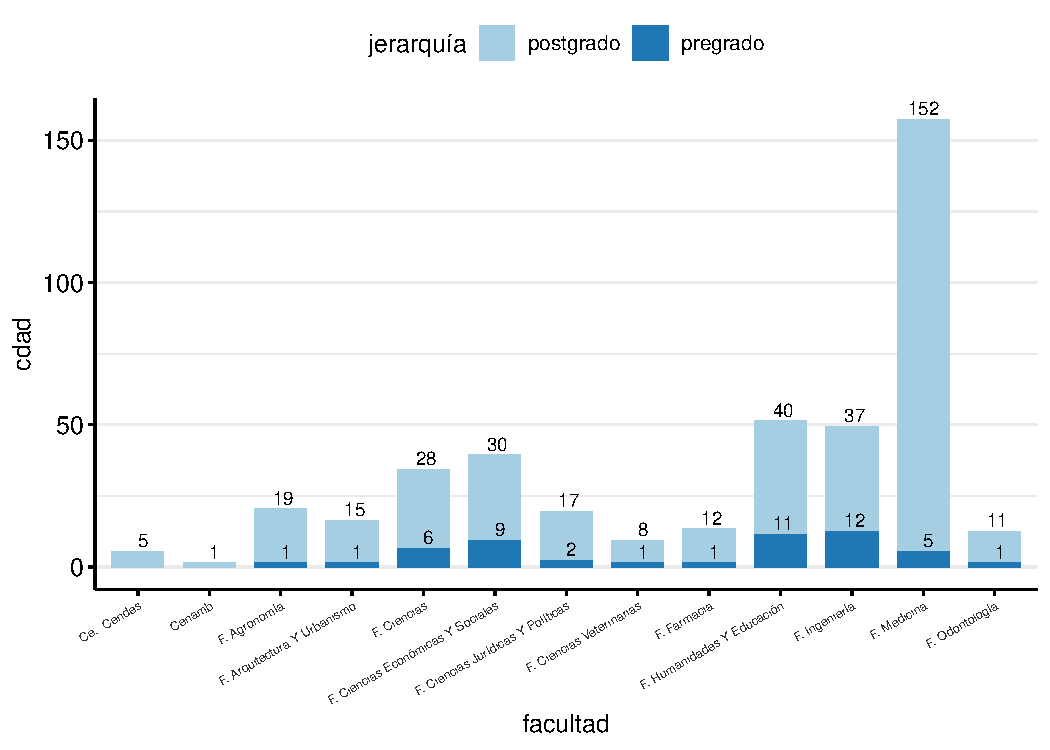
\includegraphics[width=0.7\linewidth]{_main_files/figure-latex/jerarquias-1} \caption{Total pregrados y postgrados por facultad-centro}\label{fig:jerarquias}
\end{figure}

\textbf{Aprender}

\begin{enumerate}
\def\labelenumi{\arabic{enumi}.}
\item
  En el caso de los postgrados, inicialmente se esperaba que solo estuvieran asociados a facultades pero también se encontró que el Centro de Estudios del Desarrollo y el Centro de Estudios Integrales del Ambiente imparten este tipo de estudios.

  \newpage
\item
  Se evaluó que existen nombres de postgrados duplicados con la misma categoría, lo que puede generar problemas en la clasificación de las investigaciones, teniendo como ejemplo la ``Maestría en Estadística'' que se dicta en la Facultad de Agronomía y en la Facultad de Ciencias Económicas y Sociales.
\item
  Se detectó que en pregrado existen escuelas que otorgan distintos títulos, p.~ej. de la ``Escuela de Administración y Contaduría'' se pueden obtener los títulos de ``contador'' o de ``licenciado en administración''. Esto es algo a tener presente al momento de hacer la categorización, ya que el nombre de la escuela no sirve en estos casos para realizarla, siendo necesario agregar al conjunto de datos el atributo que contenga el nombre de los títulos emitidos según la escuela.
\item
  Sobre los textos se tuvieron que realizar modificaciones ya que en los listados se encontró que algunos nombres les faltaban palabras. La revisión final de nombres, dada la cantidad total de 425 dependencias, se hizo manualmente para evitar posteriores categorizaciones erróneas.
\end{enumerate}

\hypertarget{asignacion}{%
\subsubsection{Iteración- Extracción y Clasificación de las Investigaciones}\label{asignacion}}

En esta iteración se mencionan los principales obstáculos y las estrategias implementadas para alcanzar el objetivo de realizar la clasificación de cada trabajo alojado en Saber UCV, no obstante, se omite especificar algunos de los problemas que se encontraron, ya que extenderse en esto abultaría considerablemente el contenido expuesto.

\textbf{Especulación}

Para las investigaciones que reposan en Saber UCV que cuentan con un archivo anexo, correspondiente al documento de la misma, es posible realizar la descarga, extraer una porción de texto y adoptando métodos basados en reglas de coincidencia de patrones, con las etiquetas obtenidas en la iteración anterior, ver \ref{labels}, ``Levantamiento de Categorías'', hacer la categorización por área de estudio, asignando el nombre del pre o postgrado, la escuela-postgrado y la facultad-centro de adscripción. Igualmente de esta porción de texto se estima viable extraer el nombre del tutor.

\textbf{Colaboración}

Motivado a que en la primera iteración para conformar el conjunto de datos se había obtenido el enlace asociado al documento soporte de la investigación, se procedió mediante un bucle a realizar la descarga de cada documento y extraer una cantidad de dos mil caracteres, partiendo del principio de que los trabajos de grado o tesis en sus primeras páginas tienen el nombre de la carrera o el postgrado, el nombre de la facultad-centro donde se cursó el estudio, el nombre del título al que optan y el nombre del tutor.

De igual manera, en esta iteración fue necesario realizar distintas adaptaciones para lograr la coincidencia de patrones. Teniendo en cuenta que son 425 etiquetas las que se usarán para realizar la clasificación, llegando a tener 14 palabras algunas categorías, es elevada la probabilidad de que no se pueda hacer el ``\emph{pattern matching}'' entre el texto y la etiqueta.

Lo anterior motivó a realizar un proceso de limpieza, modificación y disminución de la cantidad de palabras, tanto en las etiquetas como en el texto extraído. Se evaluó en cada adaptación cuáles razones impedían clasificar los documentos aún pendientes, se tomaron los correctivos y así se fue incrementando, de forma iterativa, la exactitud en este proceso.

También se tuvo que tomar en cuenta el orden en que se iba a ejecutar la secuencia de encontrar las coincidencias. Ejemplo de lo mencionado es que varias facultades contienen las mismas tres palabras en la parte inicial de su nombre: Facultad de Ciencias, Facultad de Ciencias Jurídicas y Políticas, Facultad de Ciencias Económicas y Sociales y la Facultad de Ciencias Veterinarias. La secuencia para hacer la detección de la coincidencia fue buscar realizar la comparación de cada elemento ordenado en forma decreciente, según el total de caracteres que tenga el nombre de la facultad, para evitar clasificaciones erróneas.

Adicionalmente, en el proceso de hacer coincidir las frases se encontraron 17 postgrados que no estaban en el conjunto de datos de las categorías, los cuales se tuvo que proceder a agregar.

Igualmente, para aquellos casos donde no se podía hacer \emph{match,} se aplicó el algoritmo ``Smith Waterman'' (\protect\hyperlink{ref-smith1981}{Smith y Waterman 1981}), expuesto en \ref{alghist}, ``Marco Teórico-Referencial'', el cual permite alinear dos cadenas de texto cuando una de ellas no tiene coincidencia absoluta con la otra, como puede pasar en este caso por la introducción de caracteres adicionales.

Otro punto a mencionar es el problema que se generó al realizar la lectura de algunos documentos en los cuales se introdujeron caracteres aleatorios en el texto de los documentos, motivado a la aparición de diversos \emph{encodings,} los cuales no resultó viable codificarlos a ``UTF-08'', haciendo que aparecieran caracteres no reconocidos dentro del texto y consecuentemente dificultando la tarea de lograr realizar el proceso de ``pattern matching''. El algorimo SW nuveamente resultó eficaz para darle solución a este problema, aunque igualmente se hicieron pruebas con otros métodos como el algoritmo ``Distancia de Levenshtein'' o variaciones de este.

Como resultado de los procesos ejecutados se obtuvo que sobre un total de 9.982 potenciales documentos se lograron clasificar 9.585 investigaciones, mientras que 244 no disponían información en el texto del documento y resultaba inviable hacer la categorización. En algunos casos la falta de información estuvo motivada en que el archivo contenía imágenes por estar escaneado el contenido o también en que los documentos anexos no fuesen trabajos de grado o tesis, sino informes de algún otro estilo.

Otro resultado que se obtuvo, a nivel de cifras agregadas, es la cantidad de categorías distintas, con al menos una investigación asignada a una facultad o centro, que ascendió a 284, que se distribuyen por facultad según lo que se observa en la Figura \ref{fig:categorias}.

\begin{figure}
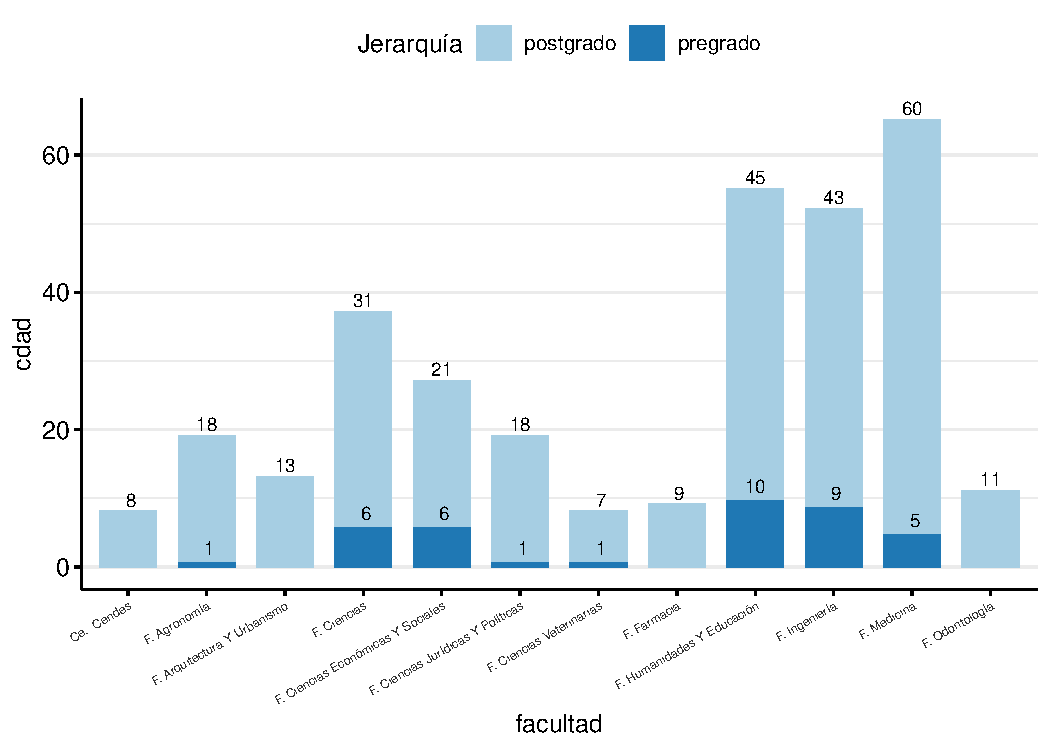
\includegraphics[width=0.8\linewidth]{_main_files/figure-latex/categorias-1} \caption{Cantidades de categorías por facultad y nivel académico}\label{fig:categorias}
\end{figure}

Para ilustar algunos de los resultados generados, en la Figura \ref{fig:totalesporfacultad}, se pueden ver primero la cantidad total de investigaciones que pudieron ser clasificadas por cada facultad - centro de estudios y en la segunda posición, la cantidad de documentos disponibles por fecha de publicación que abarcan el período 01/01/1977 al 06/15/2023.

\begin{figure}
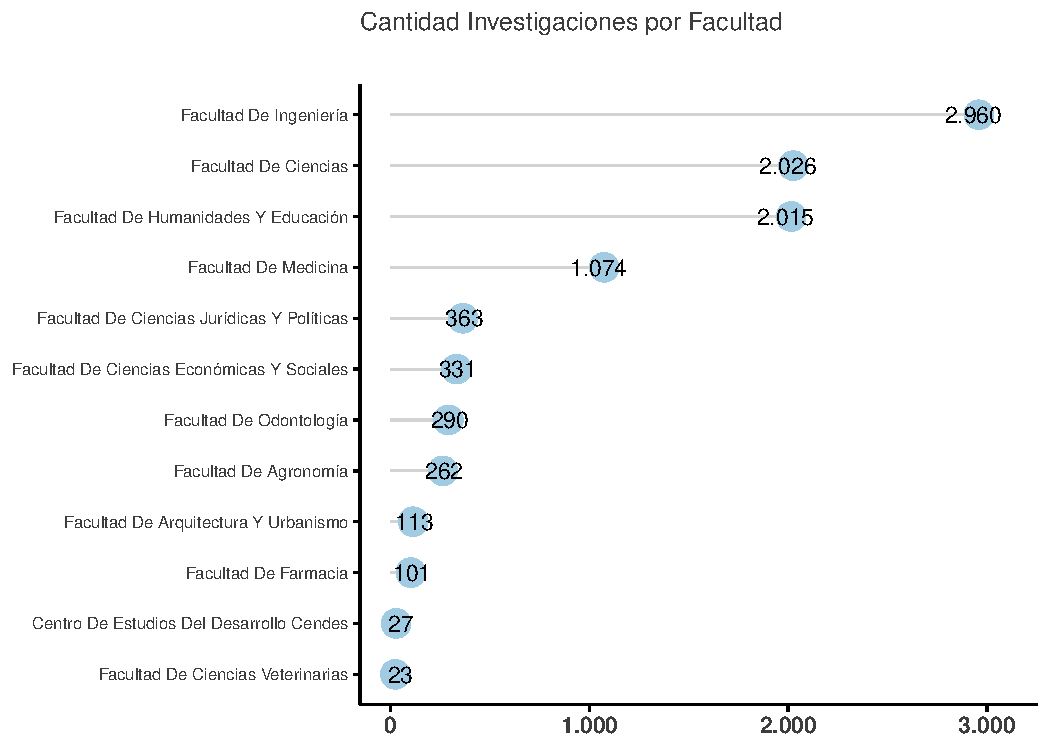
\includegraphics[width=0.48\linewidth]{_main_files/figure-latex/totalesporfacultad-1} 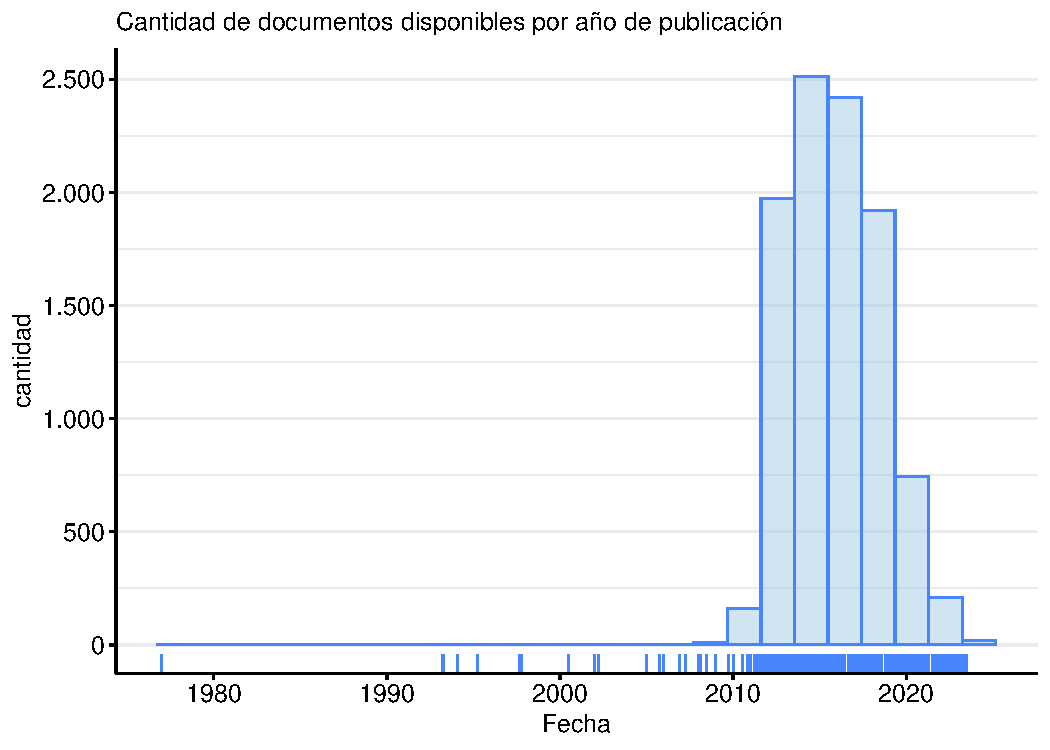
\includegraphics[width=0.48\linewidth]{_main_files/figure-latex/totalesporfacultad-2} \caption{Cantidades de investigaciones clasificadas por facultad y por año de publicación}\label{fig:totalesporfacultad}
\end{figure}

Por otra parte, en cuanto a la obtención de los nombres de los tutores, el procedimiento adoptado fue nuevamente realizar algunas limpiezas sobre el texto como remover dígitos, abreviaturas de títulos académicos (PhD, MgS, etc), y luego extraer el texto que se encontraba delimitado entre la propia palabra ``tutor'' y el brinco de línea ``\textbackslash n'' más próximo a la aparición de dicha palabra. Con el procedimiento descrito se pudo extraer un total de 7.969 nombres en la misma cantidad de investigaciones, cifra equivalente al 79,8\% del total, así como 3.718 nombres distintos \footnote{la diferencia entre la cantidad de ``nombres'' y los ``nombres distintos'' se motiva en que un mismo tutor puede haber tutoreado a más de un estudiante en la elaboración del trabajo de grado o tesis. Los nombres que aparecen más de una vez aportan mayor confianza a que el nombre se haya extraído con éxito, ya que existen múltiples coincidencias en la extracción del nombre.}.

Dentro del mismo contexto, en la Figura \ref{fig:tutores}, se aprecia el histograma que muestra la frecuencia para la cantidad de investigaciones que corresponden a un tutor que tiene un nombre coincidente, lo que se explica, p.~ej., con el valor de la segunda barra de izquierda a derecha, el cual se debe interpretar de la siguiente forma: existen 487 casos donde un tutor aparece mencionado en dos trabajos de grado.

\begin{figure}
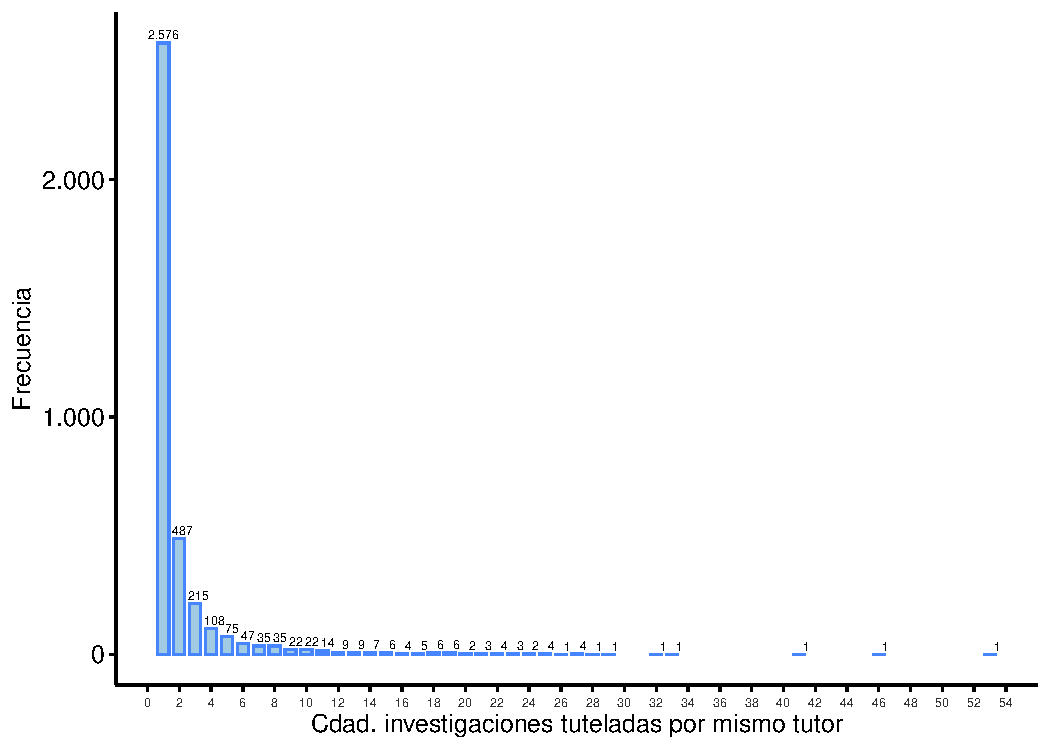
\includegraphics[width=0.9\linewidth]{_main_files/figure-latex/tutores-1} \caption{Histógrama nombres tutores extraídos }\label{fig:tutores}
\end{figure}

Con mayor nivel de detalle se tiene que, la cantidad de trabajos donde fue detectado que un tutor tuvo dos o más trabajos tutelados es 5.393, equivalente a un 54\%. La cifra anterior tiene la significancia de mostrar que para más de la mitad de los trabajos existe la certeza de que se encontró un nombre idéntico en al menos dos casos, brindando mayor confianza sobre el proceso ejecutado.

Por otro lado, en los otros 2.576 casos en que solo se encontró un tutor por investigación, al realizar un análisis exploratorio se pudo apreciar que en una variedad de casos el nombre no fue escrito en forma idéntica entre un trabajo y otro, p.~ej. dejando unicamente la inicial del segundo apellido u omitiendo el segundo nombre. Escapa al alcance de este trabajo realizar la depuración que permita consolidar más trabajos de grado al correspondiente tutor.

\textbf{Aprender}

A continuación se agrupan y enuncian los principales inconvenientes que se encontraron y se indica el aprendizaje obtenido para fases sucesivas de desarrollo:

\begin{enumerate}
\def\labelenumi{\arabic{enumi}.}
\item
  Aparición de errores en la redacción y ortografía por parte de los autores, como por ejemplo, escribir incorrectamente el nombre del título al que optan o la facultad donde realizaron los estudios. Esto implicó crear reglas para realizar reemplazos de palabras en los textos y limpiezas para facilitar el proceso de obtener la coincidencia. Un problema que se presentaría al intentar extender el SCSU a otros repositorios, cuando los trabajos de grado no estén categorizados, es que el procedimiento anterior no es completamente extrapolable si los nombres de los postgrados-escuelas y el de las facultades son distintos, ya que las reglas de modificación de texto son específicas para el corpus de la Universidad Central de Venezuela.
\item
  Cambios en el estilo y formalidades con que se deben presentar los documentos de grado en las distintas facultades o niveles académicos, cuestión que dificultó la detección de las reglas para hacer la comparación. Ante esto, se buscó encontrar las formas más genéricas en el procesamiento así como la adopción de un procedimiento que progresivamente intentaba obtener la coindicidencia: primero con el nombre del título. En caso de fallo se sigue con el nombre del pregrado o postgrado. Si nuevamente fallaba, se procedía a hacer la búsqueda del nombre de la facultad. Finalmente, si ninguna de las estrategias anteriores tenía éxito, se aplicaba el algoritmo ``Smith Waterman''.

  Con este último método se pudieron clasificar 1.658 trabajos, que equivalen a un 16,6\% del total. Es importante señalar que al aplicar este recurso se pueden generar ``falsos positivos'' y por esto en la sección \ref{pruebas}, ``Pruebas de Aceptación'', se hace una estimación estadística del error que puede representar acudir a este método.
\item
  Dentro de los archivos descargados se encontraron algunos en formato de presentaciones \emph{power point} los cuales fueron desechados solo siendo procesados los que estuviesen en formato \emph{word} o \emph{pdf} . Esto llevó a condicionar que para ejecutar la descarga y hacer el procesamiento de extracción de datos, la extensión debía ser alguna de las mencionadas como válidas\emph{.}
\item
  También se encontraron trabajos que contaban con más de un archivo disponible para descargar. En la fase inicial se descargaron 12.765 de documentos, aunque la cantidad de trabajos disponibles en el repositorio, incluyendo duplicados, era 10.843. Al evaluar las razones que motivaban que existiera una cantidad superior de archivos vs.~documentos, se distinguieron casos en que por investigación existía un archivo por capítulo y no se encontraba algún elemento que indicará la secuencia en que se debía cargar cada archivo para armar el documento unificado. Para estos casos solo se tomó el primer archivo en la lista de enlaces disponibles para tratar de hacer el proceso de clasificación.
\item
  Se hicieron algunas simplificaciones sobre postgrados que dependen de dos facultades, imputándolo solo a una, que fuese la primera en aparecer en el texto. Como queda fuera del alcance de esta investigación determinar los casos en que existe este tipo de adscripciones compartidas, se hizo esta simplificación \footnote{Un ejemplo de esto es la Maestría en Física Médica que es impartida de manera conjunta por la Facultad de Ciencias y por la Facultad de Medicina. Al no disponer de información oficial sobre otros casos de postrgrados que presenten esta característica, se adoptó el método mencionado de imputar solo a una dependencia que sea la primera en aparecer en el texto.}.
\item
  Algunos trabajos en su primera página incluyen el nombre de dos facultades o escuelas creando errores en la clasificación, p.~ej., investigaciones que indican en la portada el siguiente texto ``Facultad de Ciencias, Escuela de Computación, título: se realiza la propuesta de un sistema de gestión académica para la Escuela de Economía de la Facultad de Ciencias Económicas\ldots.'', lo cual genera mútilples clasificaciones. En estos casos se optó por realizar la imputación con base en la primera coincidencia detectada.
\item
  En la obtención del nombre del tutor es importante destacar que en varios casos el texto extraído no se corresponde propiamente al nombre del mismo, motivado a que la escritura de la portada puede responder a la representación visual. Se encontraron trabajos que tienen tutor académico, tutor industrial, cotutor y otras variantes, donde se hace una disposición en la escritura de colocar el tipo de cada tutor alíneado, cada uno en los extremos de una línea y los nombres también se disponen en los extremos de la línea superior, quebrando la regla de extracción que se había diseñando. Esto pareciera un problema a enfrentar con técnicas de segmentación de archivos que tienen en consideración la disposición visual. En el caso de esta investigación no se adoptaron métodos para abordar este problema. En las sección \ref{pruebas}, ``Pruebas de Aceptación'', se hace una evaluación estadística de la precisión alcanzada en esta extracción.
\item
  Se simplificaron algunos nombres de especializaciones por la cantidad de palabras que tienen estableciendo un límite, o \emph{prunning}, de 5 palabras para el nombre del postgrado, lo que implica que algunos trabajos habrán quedado agrupados en la misma categoría. Estos casos mayormente están asociados a las especializaciones en el área de medicina, teniendo de ejemplo la Figura \ref{fig:especial}.

  \begin{figure}

  {\centering 
\includegraphics[width=0.7\linewidth]{images/05-desarrollo/1_ciclo/especializaciones2} 

  }

  \caption{Ejemplo de nombres simplificados}\label{fig:especial}
  \end{figure}
\item
  En este proceso de clasificación no resultaba conveniente usar técnicas de aprendizaje automático dada la cantidad de categorías y el gran desbalanceo de clases.
\item
  Se detectó que en Saber UCV en la categoría que se denomina ``otros'', se encuentran documentos que corresponden a especializaciones y también se alojan 60 investigaciones que son ``trabajos de ascenso'' de profesores.
\end{enumerate}

\hypertarget{objetivos-alcanzados}{%
\subsubsection{Objetivos Alcanzados:}\label{objetivos-alcanzados}}

\begin{enumerate}
\def\labelenumi{\arabic{enumi}.}
\item
  Obtener las fichas de 9.982 investigaciones, equivalente al 100\% de los trabajos de pre y postgrado alojados en Saber UCV (descartando los duplicados), conforme a lo propuesto en el ``Objetivo Específico 1''.
\item
  Obtener 375 nombres de postgrado y 50 de carreras de pregrado, generando 454 etiquetas en total que sirvieron de insumo para alcanzar lo propuesto en el ``Objetivo Específico 2''.
\item
  Categorizar 9.585 investigaciones por área académica, equivalente al 96\% de toda la información a clasificar, de acuerdo al ``Objetivo Específico 2''.
\item
  Extraer 7.969 nombres de tutores, equivalente al 79,8\% del total de investigaciones, que también se estableció como parte del ``Objetivo Específico 2''.
\end{enumerate}

\newpage

\hypertarget{desarrollociclos3}{%
\subsection{Ciclo-Prototipo del SCSU}\label{desarrollociclos3}}

En este ciclo se abordan integralmente los diversos aspectos que permiten hacer la implementación del prototipo del SCSU con distintas iteracciones donde inicialmente se hace la preparación del corpus, se crean recomendaciones de documentos de interés, así como hace el diseño y puesta en marcha de una versión simplificada del sistema incluyendo una interfaz de usuario, un servidor para atender las peticiones y el sistema gestor de base de datos.

\hypertarget{iternlp}{%
\subsubsection{Iteración- Preparación del Corpus}\label{iternlp}}

En esta iteración el corpus conformado fue sometido a distintos procesamientos conocidos como ``preparación del corpus'' mediante la aplicación de técnicas de PLN.

\textbf{Especulación}

Creando un corpus anotado con métodos del procesamiento del lenguaje natural se facilita el acceso a información de relevancia para los investigadores mediante el análisis lingüístico de los documentos recolectados (\protect\hyperlink{ref-article}{Ruiz Fabo y Bermúdez-Sabel 2019}).

\textbf{Colaboración}

Para realizar el etiquetado de la ``parte del discurso (POS)'', se hizo una revisión exhaustiva de distintos \emph{frameworks} para realizar el anotado del corpus, como \emph{Freeling} (\protect\hyperlink{ref-padro12}{Padró y Stanilovsky 2012}), CoreNLP (\protect\hyperlink{ref-manning-etal-2014-stanford}{C. Manning et~al. 2014}), UDPipe (\protect\hyperlink{ref-UDPipe-2}{\textbf{UDPipe-2?}}) y se decidió acudir a la librería spacyr (\protect\hyperlink{ref-spacyr}{Benoit y Matsuo 2020a}) que es un \emph{wrapper} de la librería spaCy (\protect\hyperlink{ref-spacy2020}{Honnibal et~al. 2020}), que se ejecuta en el lenguaje Python. Esta librería, en lo relativo al etiquetado de las palabras por su función gramátical, lo hace acorde al marco de trabajo propuesto en la investigación ``Universal Dependencies'' (\protect\hyperlink{ref-demarneffe2021}{Marneffe et~al. 2021}). La implementación de spaCy dispone de un encadenamiento en el flujo de trabajo, resultando conveniente aplicarlo dentro del desarrollo del SCSU. Otra de las características que dispone, es contar con varios modelos preentrenados disponibles para realizar el etiquetado, e igualmente cuenta con métricas de desempeño que se encuentran dentro del estado del arte en el campo del procesamiento del lenguaje natural.

En complemento de los anterior, la librería carga el modelo preentrenado de aprendizaje automático para el idioma español denominado ``es\_core\_news\_lg''. Mediante un flujo de trabajo que se observa en la Figura \ref{fig:spacypi}, se ejecutan procesos que permiten conformar el corpus anotado.

\begin{figure}

{\centering 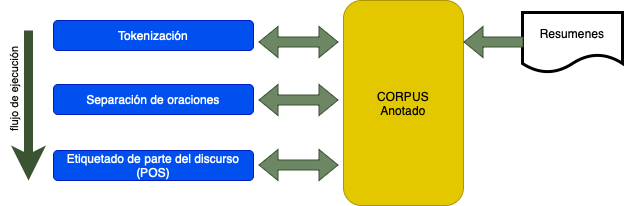
\includegraphics[width=0.8\linewidth]{images/05-desarrollo/2_ciclo/nlp/spacy_pipeline1} 

}

\caption{Arquitectura general- pipeline Spacy}\label{fig:spacypi}
\end{figure}

Ilustrativamente se muestra el texto ``\emph{\ldots{} y algunos no-metales. Contrariamente a lo\ldots{}}'', que al aplicar los métodos que dispone ``spacyr'', permite generar el corpus anotado que se puede ver en la Figura \ref{fig:corpusano}, donde se aprecia:

\begin{itemize}
\item
  Código identificador del documento.
\item
  Código identificador de la oración dentro del documento.
\item
  Código identificador del token dentro del documento.
\item
  Token.
\item
  Lema.
\item
  Etiquetado de parte del discurso (POS) para cada token.
\end{itemize}

\begin{figure}

{\centering 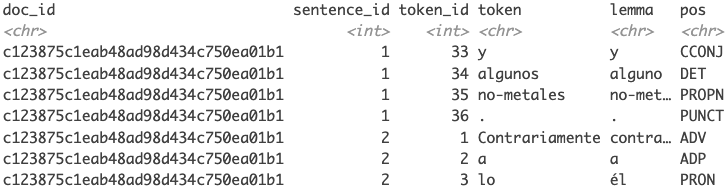
\includegraphics[width=0.9\linewidth]{images/05-desarrollo/2_ciclo/nlp/corpusanotado2} 

}

\caption{Detalle anotación del corpus}\label{fig:corpusano}
\end{figure}

Por ende, el corpus anotado cuenta con 9.982 documentos que generan 3.147.740 tokens, un vocabulario de 101.066 palabras distintas y 83.402 lemas únicos. Los tokens, agrupados por función gramatical se presentan \footnote{El proyecto Universal Dependencies disponible en el enlace \url{https://universaldependencies.org} contiene la documentación sobre las distintas funciones gramaticales que fueron etiquetadas.} en el gráfico \ref{fig:posgr} :

\begin{figure}

{\centering 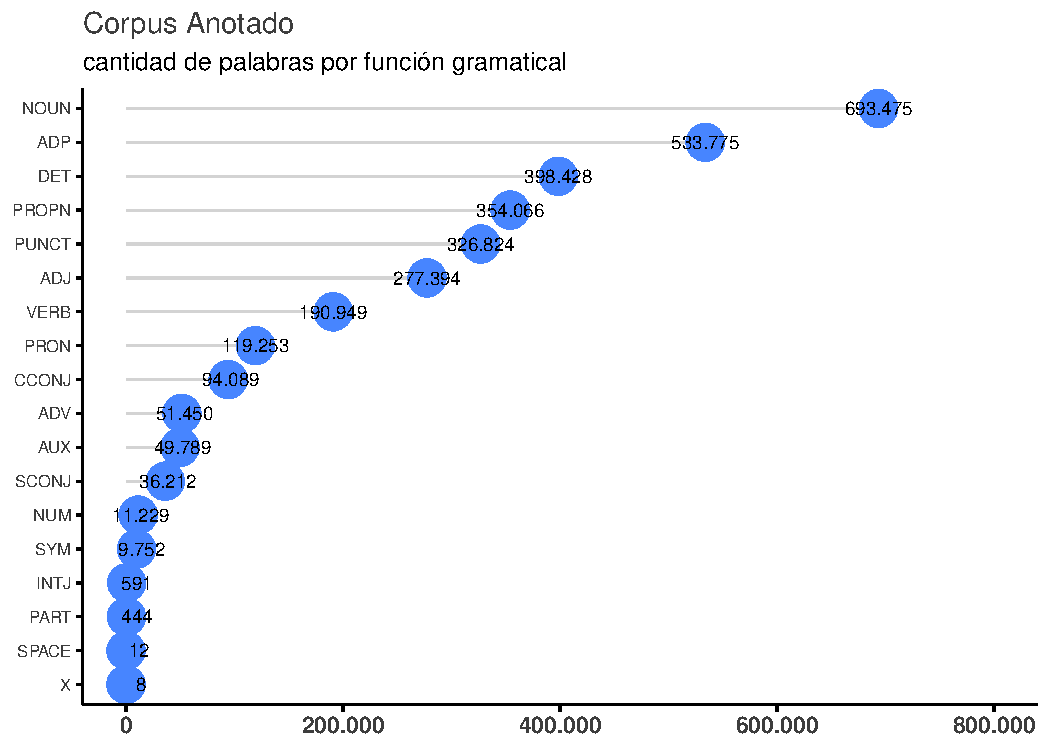
\includegraphics[width=0.7\linewidth]{_main_files/figure-latex/posgr-1} 

}

\caption{Cantidad de palabras por función gramatical}\label{fig:posgr}
\end{figure}

En el mismo orden de ideas, realizando el análisis exploratorio del corpus, es interesante ver la cantidad de palabras únicas por función gramatical y el ratio que presentan con respecto al total de palabras por ``POS'' que se vio en la Figura \ref{fig:posgr}. En la Tabla \ref{tab:lemmasg}, se observa que las categorías del ``etiquetado de la parte del discurso'' que contienen mayor cantidad de información son los nombres propios (PROPN), los adjetivos (ADJ), números (NUM) y los sustantivos (NOUN) pero los nombres propios al ser únicos en cada trabajo y los números al representar cantidades, realmente la mayor cantidad de información del corpus se encuentra en los adjetivos y sustantivos, lo que refuerza la construcción y representación de los mapas de conocimiento mediante la selección de las palabras que tienen esas funciones gramaticales.

\global\setlength{\Oldarrayrulewidth}{\arrayrulewidth}

\global\setlength{\Oldtabcolsep}{\tabcolsep}

\setlength{\tabcolsep}{0pt}

\renewcommand*{\arraystretch}{1.5}



\providecommand{\ascline}[3]{\noalign{\global\arrayrulewidth #1}\arrayrulecolor[HTML]{#2}\cline{#3}}

\begin{longtable}[c]{|p{0.93in}|p{1.04in}|p{1.34in}|p{0.77in}}

\caption{Ratio\ de\ cantidad\ única\ de\ lemas\ Vs.\ cantidad\ total\ de\ lemas}\label{tab:lemmasg}\\

\ascline{1.5pt}{666666}{1-4}

\multicolumn{1}{>{\raggedright}m{\dimexpr 0.93in+0\tabcolsep}}{\textcolor[HTML]{000000}{\fontsize{11}{11}\selectfont{\global\setmainfont{Helvetica}{\textbf{POS}}}}} & \multicolumn{1}{>{\raggedleft}m{\dimexpr 1.04in+0\tabcolsep}}{\textcolor[HTML]{000000}{\fontsize{11}{11}\selectfont{\global\setmainfont{Helvetica}{\textbf{Cantidad}}}}} & \multicolumn{1}{>{\raggedleft}m{\dimexpr 1.34in+0\tabcolsep}}{\textcolor[HTML]{000000}{\fontsize{11}{11}\selectfont{\global\setmainfont{Helvetica}{\textbf{Cdad.\ únicas}}}}} & \multicolumn{1}{>{\raggedleft}m{\dimexpr 0.77in+0\tabcolsep}}{\textcolor[HTML]{000000}{\fontsize{11}{11}\selectfont{\global\setmainfont{Helvetica}{\textbf{ratio}}}}} \\

\ascline{1.5pt}{666666}{1-4}\endfirsthead \caption[]{Ratio\ de\ cantidad\ única\ de\ lemas\ Vs.\ cantidad\ total\ de\ lemas}\label{tab:lemmasg}\\

\ascline{1.5pt}{666666}{1-4}

\multicolumn{1}{>{\raggedright}m{\dimexpr 0.93in+0\tabcolsep}}{\textcolor[HTML]{000000}{\fontsize{11}{11}\selectfont{\global\setmainfont{Helvetica}{\textbf{POS}}}}} & \multicolumn{1}{>{\raggedleft}m{\dimexpr 1.04in+0\tabcolsep}}{\textcolor[HTML]{000000}{\fontsize{11}{11}\selectfont{\global\setmainfont{Helvetica}{\textbf{Cantidad}}}}} & \multicolumn{1}{>{\raggedleft}m{\dimexpr 1.34in+0\tabcolsep}}{\textcolor[HTML]{000000}{\fontsize{11}{11}\selectfont{\global\setmainfont{Helvetica}{\textbf{Cdad.\ únicas}}}}} & \multicolumn{1}{>{\raggedleft}m{\dimexpr 0.77in+0\tabcolsep}}{\textcolor[HTML]{000000}{\fontsize{11}{11}\selectfont{\global\setmainfont{Helvetica}{\textbf{ratio}}}}} \\

\ascline{1.5pt}{666666}{1-4}\endhead



\multicolumn{1}{>{\raggedright}m{\dimexpr 0.93in+0\tabcolsep}}{\textcolor[HTML]{000000}{\fontsize{11}{11}\selectfont{\global\setmainfont{Helvetica}{PROPN}}}} & \multicolumn{1}{>{\raggedleft}m{\dimexpr 1.04in+0\tabcolsep}}{\textcolor[HTML]{000000}{\fontsize{11}{11}\selectfont{\global\setmainfont{Helvetica}{354.066}}}} & \multicolumn{1}{>{\raggedleft}m{\dimexpr 1.34in+0\tabcolsep}}{\textcolor[HTML]{000000}{\fontsize{11}{11}\selectfont{\global\setmainfont{Helvetica}{47.501}}}} & \multicolumn{1}{>{\raggedleft}m{\dimexpr 0.77in+0\tabcolsep}}{\textcolor[HTML]{4785FF}{\fontsize{11}{11}\selectfont{\global\setmainfont{Helvetica}{13,42}}}} \\

\ascline{0.75pt}{666666}{1-4}



\multicolumn{1}{>{\raggedright}m{\dimexpr 0.93in+0\tabcolsep}}{\textcolor[HTML]{000000}{\fontsize{11}{11}\selectfont{\global\setmainfont{Helvetica}{ADJ}}}} & \multicolumn{1}{>{\raggedleft}m{\dimexpr 1.04in+0\tabcolsep}}{\textcolor[HTML]{000000}{\fontsize{11}{11}\selectfont{\global\setmainfont{Helvetica}{277.394}}}} & \multicolumn{1}{>{\raggedleft}m{\dimexpr 1.34in+0\tabcolsep}}{\textcolor[HTML]{000000}{\fontsize{11}{11}\selectfont{\global\setmainfont{Helvetica}{16.584}}}} & \multicolumn{1}{>{\raggedleft}m{\dimexpr 0.77in+0\tabcolsep}}{\textcolor[HTML]{4785FF}{\fontsize{11}{11}\selectfont{\global\setmainfont{Helvetica}{5,98}}}} \\

\ascline{0.75pt}{666666}{1-4}



\multicolumn{1}{>{\raggedright}m{\dimexpr 0.93in+0\tabcolsep}}{\textcolor[HTML]{000000}{\fontsize{11}{11}\selectfont{\global\setmainfont{Helvetica}{NUM}}}} & \multicolumn{1}{>{\raggedleft}m{\dimexpr 1.04in+0\tabcolsep}}{\textcolor[HTML]{000000}{\fontsize{11}{11}\selectfont{\global\setmainfont{Helvetica}{11.229}}}} & \multicolumn{1}{>{\raggedleft}m{\dimexpr 1.34in+0\tabcolsep}}{\textcolor[HTML]{000000}{\fontsize{11}{11}\selectfont{\global\setmainfont{Helvetica}{542}}}} & \multicolumn{1}{>{\raggedleft}m{\dimexpr 0.77in+0\tabcolsep}}{\textcolor[HTML]{4785FF}{\fontsize{11}{11}\selectfont{\global\setmainfont{Helvetica}{4,83}}}} \\

\ascline{0.75pt}{666666}{1-4}



\multicolumn{1}{>{\raggedright}m{\dimexpr 0.93in+0\tabcolsep}}{\textcolor[HTML]{000000}{\fontsize{11}{11}\selectfont{\global\setmainfont{Helvetica}{NOUN}}}} & \multicolumn{1}{>{\raggedleft}m{\dimexpr 1.04in+0\tabcolsep}}{\textcolor[HTML]{000000}{\fontsize{11}{11}\selectfont{\global\setmainfont{Helvetica}{693.475}}}} & \multicolumn{1}{>{\raggedleft}m{\dimexpr 1.34in+0\tabcolsep}}{\textcolor[HTML]{000000}{\fontsize{11}{11}\selectfont{\global\setmainfont{Helvetica}{21.968}}}} & \multicolumn{1}{>{\raggedleft}m{\dimexpr 0.77in+0\tabcolsep}}{\textcolor[HTML]{4785FF}{\fontsize{11}{11}\selectfont{\global\setmainfont{Helvetica}{3,17}}}} \\

\ascline{0.75pt}{666666}{1-4}



\multicolumn{1}{>{\raggedright}m{\dimexpr 0.93in+0\tabcolsep}}{\textcolor[HTML]{000000}{\fontsize{11}{11}\selectfont{\global\setmainfont{Helvetica}{VERB}}}} & \multicolumn{1}{>{\raggedleft}m{\dimexpr 1.04in+0\tabcolsep}}{\textcolor[HTML]{000000}{\fontsize{11}{11}\selectfont{\global\setmainfont{Helvetica}{190.949}}}} & \multicolumn{1}{>{\raggedleft}m{\dimexpr 1.34in+0\tabcolsep}}{\textcolor[HTML]{000000}{\fontsize{11}{11}\selectfont{\global\setmainfont{Helvetica}{5.630}}}} & \multicolumn{1}{>{\raggedleft}m{\dimexpr 0.77in+0\tabcolsep}}{\textcolor[HTML]{4785FF}{\fontsize{11}{11}\selectfont{\global\setmainfont{Helvetica}{2,95}}}} \\

\ascline{0.75pt}{666666}{1-4}



\multicolumn{1}{>{\raggedright}m{\dimexpr 0.93in+0\tabcolsep}}{\textcolor[HTML]{000000}{\fontsize{11}{11}\selectfont{\global\setmainfont{Helvetica}{ADV}}}} & \multicolumn{1}{>{\raggedleft}m{\dimexpr 1.04in+0\tabcolsep}}{\textcolor[HTML]{000000}{\fontsize{11}{11}\selectfont{\global\setmainfont{Helvetica}{51.450}}}} & \multicolumn{1}{>{\raggedleft}m{\dimexpr 1.34in+0\tabcolsep}}{\textcolor[HTML]{000000}{\fontsize{11}{11}\selectfont{\global\setmainfont{Helvetica}{1.364}}}} & \multicolumn{1}{>{\raggedleft}m{\dimexpr 0.77in+0\tabcolsep}}{\textcolor[HTML]{4785FF}{\fontsize{11}{11}\selectfont{\global\setmainfont{Helvetica}{2,65}}}} \\

\ascline{0.75pt}{666666}{1-4}



\multicolumn{1}{>{\raggedright}m{\dimexpr 0.93in+0\tabcolsep}}{\textcolor[HTML]{000000}{\fontsize{11}{11}\selectfont{\global\setmainfont{Helvetica}{SYM}}}} & \multicolumn{1}{>{\raggedleft}m{\dimexpr 1.04in+0\tabcolsep}}{\textcolor[HTML]{000000}{\fontsize{11}{11}\selectfont{\global\setmainfont{Helvetica}{9.752}}}} & \multicolumn{1}{>{\raggedleft}m{\dimexpr 1.34in+0\tabcolsep}}{\textcolor[HTML]{000000}{\fontsize{11}{11}\selectfont{\global\setmainfont{Helvetica}{93}}}} & \multicolumn{1}{>{\raggedleft}m{\dimexpr 0.77in+0\tabcolsep}}{\textcolor[HTML]{4785FF}{\fontsize{11}{11}\selectfont{\global\setmainfont{Helvetica}{0,95}}}} \\

\ascline{0.75pt}{666666}{1-4}



\multicolumn{1}{>{\raggedright}m{\dimexpr 0.93in+0\tabcolsep}}{\textcolor[HTML]{000000}{\fontsize{11}{11}\selectfont{\global\setmainfont{Helvetica}{AUX}}}} & \multicolumn{1}{>{\raggedleft}m{\dimexpr 1.04in+0\tabcolsep}}{\textcolor[HTML]{000000}{\fontsize{11}{11}\selectfont{\global\setmainfont{Helvetica}{49.789}}}} & \multicolumn{1}{>{\raggedleft}m{\dimexpr 1.34in+0\tabcolsep}}{\textcolor[HTML]{000000}{\fontsize{11}{11}\selectfont{\global\setmainfont{Helvetica}{166}}}} & \multicolumn{1}{>{\raggedleft}m{\dimexpr 0.77in+0\tabcolsep}}{\textcolor[HTML]{4785FF}{\fontsize{11}{11}\selectfont{\global\setmainfont{Helvetica}{0,33}}}} \\

\ascline{0.75pt}{666666}{1-4}



\multicolumn{1}{>{\raggedright}m{\dimexpr 0.93in+0\tabcolsep}}{\textcolor[HTML]{000000}{\fontsize{11}{11}\selectfont{\global\setmainfont{Helvetica}{PRON}}}} & \multicolumn{1}{>{\raggedleft}m{\dimexpr 1.04in+0\tabcolsep}}{\textcolor[HTML]{000000}{\fontsize{11}{11}\selectfont{\global\setmainfont{Helvetica}{119.253}}}} & \multicolumn{1}{>{\raggedleft}m{\dimexpr 1.34in+0\tabcolsep}}{\textcolor[HTML]{000000}{\fontsize{11}{11}\selectfont{\global\setmainfont{Helvetica}{287}}}} & \multicolumn{1}{>{\raggedleft}m{\dimexpr 0.77in+0\tabcolsep}}{\textcolor[HTML]{4785FF}{\fontsize{11}{11}\selectfont{\global\setmainfont{Helvetica}{0,24}}}} \\

\ascline{0.75pt}{666666}{1-4}



\multicolumn{1}{>{\raggedright}m{\dimexpr 0.93in+0\tabcolsep}}{\textcolor[HTML]{000000}{\fontsize{11}{11}\selectfont{\global\setmainfont{Helvetica}{CCONJ}}}} & \multicolumn{1}{>{\raggedleft}m{\dimexpr 1.04in+0\tabcolsep}}{\textcolor[HTML]{000000}{\fontsize{11}{11}\selectfont{\global\setmainfont{Helvetica}{94.089}}}} & \multicolumn{1}{>{\raggedleft}m{\dimexpr 1.34in+0\tabcolsep}}{\textcolor[HTML]{000000}{\fontsize{11}{11}\selectfont{\global\setmainfont{Helvetica}{138}}}} & \multicolumn{1}{>{\raggedleft}m{\dimexpr 0.77in+0\tabcolsep}}{\textcolor[HTML]{4785FF}{\fontsize{11}{11}\selectfont{\global\setmainfont{Helvetica}{0,15}}}} \\

\ascline{0.75pt}{666666}{1-4}



\multicolumn{1}{>{\raggedright}m{\dimexpr 0.93in+0\tabcolsep}}{\textcolor[HTML]{000000}{\fontsize{11}{11}\selectfont{\global\setmainfont{Helvetica}{SCONJ}}}} & \multicolumn{1}{>{\raggedleft}m{\dimexpr 1.04in+0\tabcolsep}}{\textcolor[HTML]{000000}{\fontsize{11}{11}\selectfont{\global\setmainfont{Helvetica}{36.212}}}} & \multicolumn{1}{>{\raggedleft}m{\dimexpr 1.34in+0\tabcolsep}}{\textcolor[HTML]{000000}{\fontsize{11}{11}\selectfont{\global\setmainfont{Helvetica}{45}}}} & \multicolumn{1}{>{\raggedleft}m{\dimexpr 0.77in+0\tabcolsep}}{\textcolor[HTML]{4785FF}{\fontsize{11}{11}\selectfont{\global\setmainfont{Helvetica}{0,12}}}} \\

\ascline{0.75pt}{666666}{1-4}



\multicolumn{1}{>{\raggedright}m{\dimexpr 0.93in+0\tabcolsep}}{\textcolor[HTML]{000000}{\fontsize{11}{11}\selectfont{\global\setmainfont{Helvetica}{PUNCT}}}} & \multicolumn{1}{>{\raggedleft}m{\dimexpr 1.04in+0\tabcolsep}}{\textcolor[HTML]{000000}{\fontsize{11}{11}\selectfont{\global\setmainfont{Helvetica}{326.824}}}} & \multicolumn{1}{>{\raggedleft}m{\dimexpr 1.34in+0\tabcolsep}}{\textcolor[HTML]{000000}{\fontsize{11}{11}\selectfont{\global\setmainfont{Helvetica}{236}}}} & \multicolumn{1}{>{\raggedleft}m{\dimexpr 0.77in+0\tabcolsep}}{\textcolor[HTML]{4785FF}{\fontsize{11}{11}\selectfont{\global\setmainfont{Helvetica}{0,07}}}} \\

\ascline{0.75pt}{666666}{1-4}



\multicolumn{1}{>{\raggedright}m{\dimexpr 0.93in+0\tabcolsep}}{\textcolor[HTML]{000000}{\fontsize{11}{11}\selectfont{\global\setmainfont{Helvetica}{DET}}}} & \multicolumn{1}{>{\raggedleft}m{\dimexpr 1.04in+0\tabcolsep}}{\textcolor[HTML]{000000}{\fontsize{11}{11}\selectfont{\global\setmainfont{Helvetica}{398.428}}}} & \multicolumn{1}{>{\raggedleft}m{\dimexpr 1.34in+0\tabcolsep}}{\textcolor[HTML]{000000}{\fontsize{11}{11}\selectfont{\global\setmainfont{Helvetica}{246}}}} & \multicolumn{1}{>{\raggedleft}m{\dimexpr 0.77in+0\tabcolsep}}{\textcolor[HTML]{4785FF}{\fontsize{11}{11}\selectfont{\global\setmainfont{Helvetica}{0,06}}}} \\

\ascline{0.75pt}{666666}{1-4}



\multicolumn{1}{>{\raggedright}m{\dimexpr 0.93in+0\tabcolsep}}{\textcolor[HTML]{000000}{\fontsize{11}{11}\selectfont{\global\setmainfont{Helvetica}{ADP}}}} & \multicolumn{1}{>{\raggedleft}m{\dimexpr 1.04in+0\tabcolsep}}{\textcolor[HTML]{000000}{\fontsize{11}{11}\selectfont{\global\setmainfont{Helvetica}{533.775}}}} & \multicolumn{1}{>{\raggedleft}m{\dimexpr 1.34in+0\tabcolsep}}{\textcolor[HTML]{000000}{\fontsize{11}{11}\selectfont{\global\setmainfont{Helvetica}{262}}}} & \multicolumn{1}{>{\raggedleft}m{\dimexpr 0.77in+0\tabcolsep}}{\textcolor[HTML]{4785FF}{\fontsize{11}{11}\selectfont{\global\setmainfont{Helvetica}{0,05}}}} \\

\ascline{1.5pt}{666666}{1-4}



\end{longtable}



\arrayrulecolor[HTML]{000000}

\global\setlength{\arrayrulewidth}{\Oldarrayrulewidth}

\global\setlength{\tabcolsep}{\Oldtabcolsep}

\renewcommand*{\arraystretch}{1}

Por otra parte se tiene que, contar con un corpus anotado permite ir inspeccionando los patrones que se presentan en él. Un ejemplo se tiene en la Figura \ref{fig:compurake}, donde mediante el método \emph{Rake}, que basado en la determinación de la frecuencia de palabras y patrones co-ocurrentes, logra extraer términos clave, en este caso para las palabras clave asociadas al subconjunto de trabajos que fueron realizados en la Escuela de Computación.

\begin{figure}

{\centering 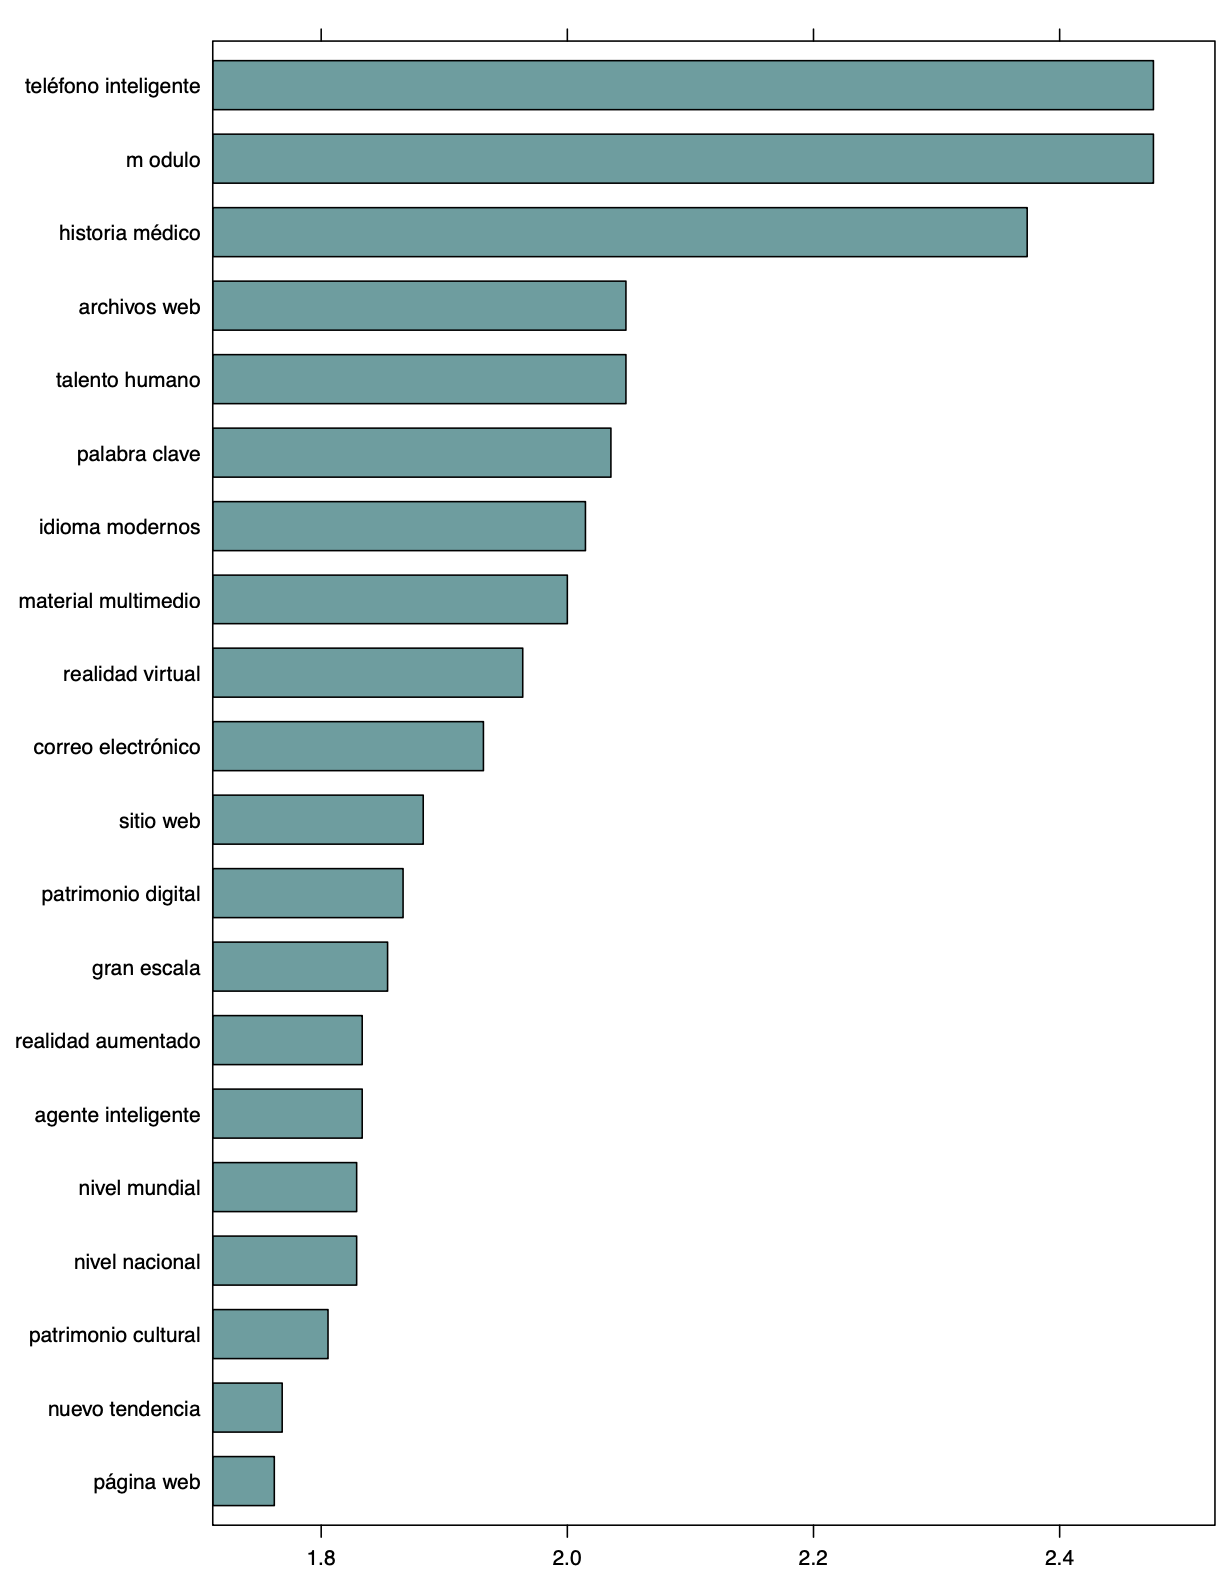
\includegraphics[width=0.6\linewidth]{images/05-desarrollo/2_ciclo/nlp/computacion_noun_adj} 

}

\caption{Palabras clave en investigaciones de la Escuela de Computación}\label{fig:compurake}
\end{figure}

Cabe destacar que la tabla que conforma el corpus anotado para esta fase de la investigación, se alojó en memoria RAM en una estructura de datos tabular denominada \emph{dataframe} del lenguaje R, sin ser registrada en un gestor de base de datos.

\textbf{Aprender}

Al analizar el corpus anotado se detectaron algunos puntos a considerar para análisis posteriores.

\begin{itemize}
\item
  El proceso de separación por tokens y de lematización, como ya se mencionó, se hizo con la librería spacyr, que hace estos procesos mediante el uso de un modelo preentrenado de aprendizaje automático. Hubo ciertos términos que son muy específicos de un área de conocimiento, como en la química, donde los \emph{c}ompuestos, moléculas, nomenclaturas u otros, contienen denominaciones conformadas por cadenas de letras mayúsculas seguidas de puntos, que no presentan estructuras gramaticales propias del lenguaje natural, sino de un dominio específico, ver Figura \ref{fig:quimica}. Al tener un modelo intentando hacer la separación de los tokens o el etiquetado bajo unos textos con los cuales no fue entrenado, el proceso falla en la ejecución de sus tareas. Este problema, para ese tipo de términos, no fue resuelto al no disponer con un modelo entrenado para este dominio. En investigaciones posteriores pudiera realizarse un sobreentrenamiento que incluyera el etiquetado de estos \emph{tokens} de dominios muy especializados, como generalmente se presenta en carreras científicas y así poder mejorar la fase del etiquetado de las funciones gramaticales (POS).

  \begin{figure}

  {\centering 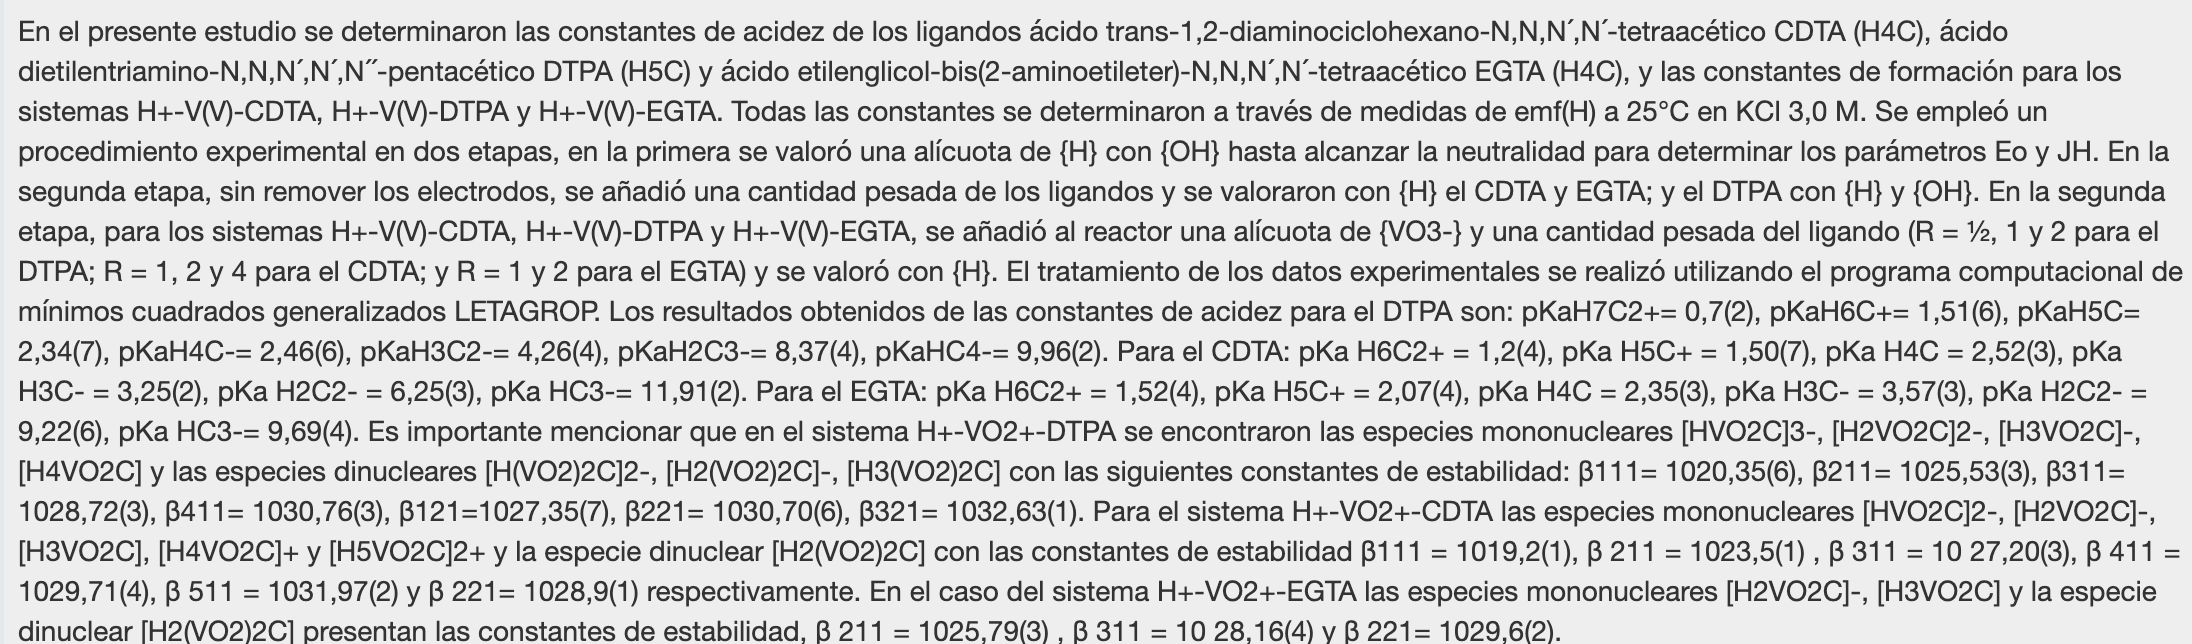
\includegraphics[width=0.9\linewidth]{images/05-desarrollo/2_ciclo/quimica} 

  }

  \caption{Texto "resumen" de trabajo de grado de Maestría en Química. Autora: Margarita González}\label{fig:quimica}
  \end{figure}
\item
  La lematización permitió reducir en un 17,5 \% el vocabulario al pasar de 101.066 palabras a 83.402 lemas. Específicamente los lemas que se van a usar en fases posteriores del análisis son los que están categorizados en el etiquetado del discurso como ``ADJ'' (adjetivos) que totalizan 277.394, equivalentes a un 8,8\% del total de palabras y los ``NOUMS'' (sustantivos) son 693.475 equivalentes al 22\% de las palabras presentes en el corpus. En el registro en base de datos se conservará completo el corpus anotado, independientemente de la función gramatical.
\item
  Los textos del ``resumen'' que se encuentran en la ficha de cada trabajo alojado en Saber UCV, en 396 casos, equivalentes al 4.3\% del total, contienen una porción de texto en idioma inglés referente al ``abstract'', siendo óptimo aislar únicamente las partes que se encuentran en idioma español para que funcione correctamente el ``etiquetado de la parte del discurso''.
\end{itemize}

\hypertarget{imrecomendacion}{%
\subsubsection{Iteración - Recomendación Documentos}\label{imrecomendacion}}

En esta iteración se revisó la creación de recomendaciones de investigaciones, basándose en la similitud que presente un documento con el resto de los documentos que conformal el corpus.

\textbf{Especulación}

Se ha determinado que los investigadores no necesariamente realizan la búsqueda de documentos que le puedan ser de interés mediante un \emph{query} que contenga términos clave, sino a partir de un documento que les resulta de interés, quieren localizar otros que puedan compartir ciertos aspectos (\protect\hyperlink{ref-zhou2018}{Zhou, Zhou, y Xu 2018}).

Dentro de este contexto se tiene que, la similitud de un documento con otro se puede entender en esta implementación, como aquellos que tienden a compartir palabras y dentro de una ``\emph{term document matrix}'' generan vectores similares (\protect\hyperlink{ref-jurafsky2009}{Jurafsky y Martin 2009}). Es por esto que se considera que los documentos que presenten mayor similitud pueden resultar de interés para los investigadores, expandiendo así las posibilidades de inspección del corpus.

\textbf{Colaboración}

Mediante la creación de una \emph{``term document matrix''}, usando el \emph{framework} para análisis cuantitativo de textos quanteda (\protect\hyperlink{ref-quanteda}{Benoit et~al. 2018a}), la matriz obtenida refleja características esenciales de los documentos, en lo relativo a las palabras que lo conforman y su frecuencia.



En cada fila de la matriz se representa un documento, también equivalente a un vector. Midiendo la similitud \emph{coseno}, revisada en \ref{similitud}, con la función ``\texttt{textstat\_simil}'', entre un determinado documento y el resto de los que conforman el corpus, es viable determinar cuáles son los más ``parecidos''.

Se realizó un proceso iterativo para calcular la similitud coseno entre documentos y se pudo apreciar que los resultados de similitud pueden resultar de interés en diversos casos, como el que se muestra en la Figura \ref{fig:similitudreco}.

\begin{figure}

{\centering 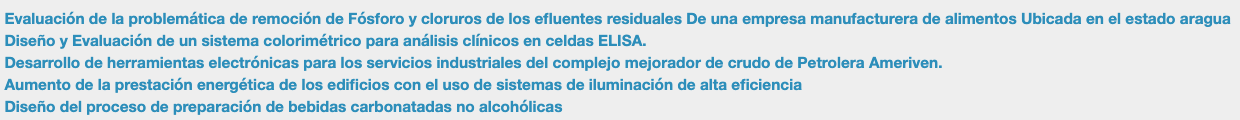
\includegraphics[width=0.9\linewidth]{images/05-desarrollo/2_ciclo/similitud_reco2} 

}

\caption{Resultado de recomendaciones al documento: "Diseño de un sistema para la desinfección de aguas de consumo humano y de uso industrial empleando un material inorgánico antibacterial"}\label{fig:similitudreco}
\end{figure}

\textbf{Aprendizaje:}

Es necesario señalar que el método adaptado no se considera que esté dentro del ``estado del arte'' para realizar recomendaciones, no obstante, se hace la evaluación de este recurso dentro del SCSU al ser de sencilla implementación, cálculos rápidos, robustos que no consumen mayores recursos computacionales, los cuales quedan disponibles para otras tareas que ejecuta el SCSU.

\hypertarget{iterbol}{%
\subsubsection{Iteración- Implementación Prototipo}\label{iterbol}}

En esta iteración se hace el desarrollo del prototipo de un ``sistema de recuperación de información'' que servirá de base para probar distintas funcionalidades con las cuales contará el Sistema Complementario Saber UCV. En particular se hace el prototipo de la aplicación web, mediante el uso del \emph{framework} Shiny y se establecen los casos de uso para que el usuario pueda realizar procesos de búsqueda sobre el corpus anotado que se conformó anteriormente, ver \ref{iternlp}, ``Preparación del Corpus''.

Especificamente, en este prototipo solo se va a trabajar con el subconjunto de las investigaciones que han sido realizadas en la Facultad de Ciencias y ante un \emph{query} son extraídos los documentos que contengan tales palabras y con ellos se representan los mapas de conocimiento.

Igualmente se tiene que, esta implementación se apoya en el uso del sistema gestor de base de datos PostgreSQL, ya que este \emph{software} nativamente cuenta con la funcionalidad de construir un índice invertido, sobre un conjunto de documentos y así se da sustento a las ``búsquedas de texto completo''.

\textbf{Especulación}

Contar con un prototipo permitirá evaluar las posibles interacciones entre el usuario y la versión que se adopte para estar en producción del Sistema Complementario Saber UCV, así como analizar los tiempos de respuesta y los resultados de las visualizaciones.

Dentro de los planteado se tiene que, para el desarrollo de este prototipo se seleccionan los textos resúmenes que fueron categorizados como pertenecientes a la Facultad de Ciencias.

Durante la fase de especulación de este ciclo se realizaron los diagramas de caso de uso que se ven en las figuras \ref{fig:protoUC1} y \ref{fig:protoUC11}:

\newpage

\begin{figure}

{\centering 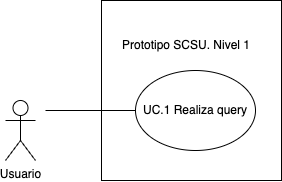
\includegraphics[width=0.45\linewidth]{images/05-desarrollo/2_ciclo/UC/prototipo_nivel1} 

}

\caption{Caso de Uso 1 - Prototipo SCSU - nivel 1}\label{fig:protoUC1}
\end{figure}

\begin{figure}

{\centering 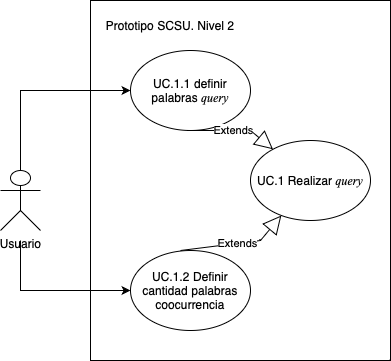
\includegraphics[width=0.45\linewidth]{images/05-desarrollo/2_ciclo/UC/prototipo_nivel2} 

}

\caption{Caso de uso 1.1 - Prototipo SCSU - nivel 2}\label{fig:protoUC11}
\end{figure}

En el Cuadro \ref{tab:prototipoUC1}, se muestra el caso de uso UC.1 de prototipo del SCSU.

\newpage

\global\setlength{\Oldarrayrulewidth}{\arrayrulewidth}

\global\setlength{\Oldtabcolsep}{\tabcolsep}

\setlength{\tabcolsep}{0pt}

\renewcommand*{\arraystretch}{1.5}



\providecommand{\ascline}[3]{\noalign{\global\arrayrulewidth #1}\arrayrulecolor[HTML]{#2}\cline{#3}}

\begin{longtable}[c]{|p{1.00in}|p{6.00in}}

\caption{Prototipo\ SCSU\ UC.1}\label{tab:prototipoUC1}\\

\hhline{>{\arrayrulecolor[HTML]{666666}\global\arrayrulewidth=0.75pt}->{\arrayrulecolor[HTML]{666666}\global\arrayrulewidth=0.75pt}-}

\multicolumn{1}{!{\color[HTML]{666666}\vrule width 0.75pt}>{\cellcolor[HTML]{C2C2C2}\raggedright}m{\dimexpr 1in+0\tabcolsep}}{\textcolor[HTML]{000000}{\fontsize{10}{10}\selectfont{\global\setmainfont{Helvetica}{Nombre}}}} & \multicolumn{1}{!{\color[HTML]{666666}\vrule width 0.75pt}>{\raggedright}m{\dimexpr 6in+0\tabcolsep}!{\color[HTML]{666666}\vrule width 0.75pt}}{\textcolor[HTML]{000000}{\fontsize{10}{10}\selectfont{\global\setmainfont{Helvetica}{UC.1:\ Realizar\ proceso\ de\ recuperación\ de\ información\ (query)}}}} \\

\noalign{\global\arrayrulewidth 0.75pt}\arrayrulecolor[HTML]{666666}

\hhline{|>{\arrayrulecolor[HTML]{666666}\global\arrayrulewidth=0.75pt}-|>{\arrayrulecolor[HTML]{666666}\global\arrayrulewidth=0.75pt}-}



\multicolumn{1}{!{\color[HTML]{666666}\vrule width 0.75pt}>{\cellcolor[HTML]{C2C2C2}\raggedright}m{\dimexpr 1in+0\tabcolsep}}{\textcolor[HTML]{000000}{\fontsize{10}{10}\selectfont{\global\setmainfont{Helvetica}{Descripción}}}} & \multicolumn{1}{!{\color[HTML]{666666}\vrule width 0.75pt}>{\raggedright}m{\dimexpr 6in+0\tabcolsep}!{\color[HTML]{666666}\vrule width 0.75pt}}{\textcolor[HTML]{000000}{\fontsize{10}{10}\selectfont{\global\setmainfont{Helvetica}{El\ usuario\ realiza\ búsquedas\ sobre\ los\ textos\ que\ conforman\ el\ corpus\ del\ prototipo}}}} \\

\noalign{\global\arrayrulewidth 0.75pt}\arrayrulecolor[HTML]{666666}

\hhline{|>{\arrayrulecolor[HTML]{666666}\global\arrayrulewidth=0.75pt}-|>{\arrayrulecolor[HTML]{666666}\global\arrayrulewidth=0.75pt}-}



\multicolumn{1}{!{\color[HTML]{666666}\vrule width 0.75pt}>{\cellcolor[HTML]{C2C2C2}\raggedright}m{\dimexpr 1in+0\tabcolsep}}{\textcolor[HTML]{000000}{\fontsize{10}{10}\selectfont{\global\setmainfont{Helvetica}{Actor}}}} & \multicolumn{1}{!{\color[HTML]{666666}\vrule width 0.75pt}>{\raggedright}m{\dimexpr 6in+0\tabcolsep}!{\color[HTML]{666666}\vrule width 0.75pt}}{\textcolor[HTML]{000000}{\fontsize{10}{10}\selectfont{\global\setmainfont{Helvetica}{Usuario}}}} \\

\noalign{\global\arrayrulewidth 0.75pt}\arrayrulecolor[HTML]{666666}

\hhline{|>{\arrayrulecolor[HTML]{666666}\global\arrayrulewidth=0.75pt}-|>{\arrayrulecolor[HTML]{666666}\global\arrayrulewidth=0.75pt}-}



\multicolumn{2}{!{\color[HTML]{666666}\vrule width 0.75pt}>{\cellcolor[HTML]{8F8F8F}\centering}m{\dimexpr 7in+2\tabcolsep+0.75pt}!{\color[HTML]{666666}\vrule width 0.75pt}}{\textcolor[HTML]{000000}{\fontsize{10}{10}\selectfont{\global\setmainfont{Helvetica}{Flujo\ de\ Eventos}}}} \\

\noalign{\global\arrayrulewidth 0.75pt}\arrayrulecolor[HTML]{666666}

\hhline{|>{\arrayrulecolor[HTML]{666666}\global\arrayrulewidth=0.75pt}-|>{\arrayrulecolor[HTML]{666666}\global\arrayrulewidth=0.75pt}-}



\multicolumn{2}{!{\color[HTML]{666666}\vrule width 0.75pt}>{\cellcolor[HTML]{A3A3A3}\raggedright}m{\dimexpr 7in+2\tabcolsep+0.75pt}!{\color[HTML]{666666}\vrule width 0.75pt}}{\textcolor[HTML]{000000}{\fontsize{10}{10}\selectfont{\global\setmainfont{Helvetica}{Flujo\ Básico}}}} \\

\noalign{\global\arrayrulewidth 0.75pt}\arrayrulecolor[HTML]{666666}

\hhline{|>{\arrayrulecolor[HTML]{666666}\global\arrayrulewidth=0.75pt}-|>{\arrayrulecolor[HTML]{666666}\global\arrayrulewidth=0.75pt}-}



\multicolumn{2}{!{\color[HTML]{666666}\vrule width 0.75pt}>{\raggedright}m{\dimexpr 7in+2\tabcolsep+0.75pt}!{\color[HTML]{666666}\vrule width 0.75pt}}{\textcolor[HTML]{000000}{\fontsize{10}{10}\selectfont{\global\setmainfont{Helvetica}{El\ caso\ de\ uso\ inicia\ cuando\ el\ usuario\ ingresa\ a\ la\ aplicación\ y\ el\ prototipo\ muesta\ dos\ campos:\ }}}\textcolor[HTML]{000000}{\fontsize{10}{10}\selectfont{\global\setmainfont{Helvetica}{\linebreak }}}\textcolor[HTML]{000000}{\fontsize{10}{10}\selectfont{\global\setmainfont{Helvetica}{\ 1)\ En\ el\ primero\ debe\ introducir\ el\ texto\ a\ buscar.\ }}}\textcolor[HTML]{000000}{\fontsize{10}{10}\selectfont{\global\setmainfont{Helvetica}{\linebreak }}}\textcolor[HTML]{000000}{\fontsize{10}{10}\selectfont{\global\setmainfont{Helvetica}{\ 2)\ En\ el\ segundo,\ en\ el\ que\ aparece\ por\ defecto\ el\ valor\ 60,\ se\ corresponde\ con\ las\ cantidades\ de\ coocurrencias\ que\ serán\ presentadas\ en\ los\ \ mapas\ de\ conocimiento.\ }}}\textcolor[HTML]{000000}{\fontsize{10}{10}\selectfont{\global\setmainfont{Helvetica}{\linebreak }}}\textcolor[HTML]{000000}{\fontsize{10}{10}\selectfont{\global\setmainfont{Helvetica}{\ 3)\ El\ usuario\ hace\ clic\ en\ el\ "buscar\ palabras"\ }}}\textcolor[HTML]{000000}{\fontsize{10}{10}\selectfont{\global\setmainfont{Helvetica}{\linebreak }}}\textcolor[HTML]{000000}{\fontsize{10}{10}\selectfont{\global\setmainfont{Helvetica}{\ 4)\ El\ prototipo\ presenta\ los\ resultados\ obtenidos\ }}}\textcolor[HTML]{000000}{\fontsize{10}{10}\selectfont{\global\setmainfont{Helvetica}{\linebreak }}}\textcolor[HTML]{000000}{\fontsize{10}{10}\selectfont{\global\setmainfont{Helvetica}{\ 5)\ El\ caso\ de\ uso\ termina}}}} \\

\noalign{\global\arrayrulewidth 0.75pt}\arrayrulecolor[HTML]{666666}

\hhline{|>{\arrayrulecolor[HTML]{666666}\global\arrayrulewidth=0.75pt}-|>{\arrayrulecolor[HTML]{666666}\global\arrayrulewidth=0.75pt}-}



\multicolumn{2}{!{\color[HTML]{666666}\vrule width 0.75pt}>{\cellcolor[HTML]{A3A3A3}\raggedright}m{\dimexpr 7in+2\tabcolsep+0.75pt}!{\color[HTML]{666666}\vrule width 0.75pt}}{\textcolor[HTML]{000000}{\fontsize{10}{10}\selectfont{\global\setmainfont{Helvetica}{Flujo\ Alternativo}}}} \\

\noalign{\global\arrayrulewidth 0.75pt}\arrayrulecolor[HTML]{666666}

\hhline{|>{\arrayrulecolor[HTML]{666666}\global\arrayrulewidth=0.75pt}-|>{\arrayrulecolor[HTML]{666666}\global\arrayrulewidth=0.75pt}-}



\multicolumn{1}{!{\color[HTML]{666666}\vrule width 0.75pt}>{\cellcolor[HTML]{C2C2C2}\raggedright}m{\dimexpr 1in+0\tabcolsep}}{\textcolor[HTML]{000000}{\fontsize{10}{10}\selectfont{\global\setmainfont{Helvetica}{Título}}}} & \multicolumn{1}{!{\color[HTML]{666666}\vrule width 0.75pt}>{\cellcolor[HTML]{C2C2C2}\raggedright}m{\dimexpr 6in+0\tabcolsep}!{\color[HTML]{666666}\vrule width 0.75pt}}{\textcolor[HTML]{000000}{\fontsize{10}{10}\selectfont{\global\setmainfont{Helvetica}{Descripción}}}} \\

\noalign{\global\arrayrulewidth 0.75pt}\arrayrulecolor[HTML]{666666}

\hhline{|>{\arrayrulecolor[HTML]{666666}\global\arrayrulewidth=0.75pt}-|>{\arrayrulecolor[HTML]{666666}\global\arrayrulewidth=0.75pt}-}



\multicolumn{1}{!{\color[HTML]{666666}\vrule width 0.75pt}>{\raggedright}m{\dimexpr 1in+0\tabcolsep}}{\textcolor[HTML]{000000}{\fontsize{10}{10}\selectfont{\global\setmainfont{Helvetica}{N/A}}}} & \multicolumn{1}{!{\color[HTML]{666666}\vrule width 0.75pt}>{\raggedright}m{\dimexpr 6in+0\tabcolsep}!{\color[HTML]{666666}\vrule width 0.75pt}}{\textcolor[HTML]{000000}{\fontsize{10}{10}\selectfont{\global\setmainfont{Helvetica}{N/A}}}} \\

\noalign{\global\arrayrulewidth 0.75pt}\arrayrulecolor[HTML]{666666}

\hhline{|>{\arrayrulecolor[HTML]{666666}\global\arrayrulewidth=0.75pt}-|>{\arrayrulecolor[HTML]{666666}\global\arrayrulewidth=0.75pt}-}



\multicolumn{2}{!{\color[HTML]{666666}\vrule width 0.75pt}>{\cellcolor[HTML]{A3A3A3}\centering}m{\dimexpr 7in+2\tabcolsep+0.75pt}!{\color[HTML]{666666}\vrule width 0.75pt}}{\textcolor[HTML]{000000}{\fontsize{10}{10}\selectfont{\global\setmainfont{Helvetica}{Precondiciones}}}} \\

\noalign{\global\arrayrulewidth 0.75pt}\arrayrulecolor[HTML]{666666}

\hhline{|>{\arrayrulecolor[HTML]{666666}\global\arrayrulewidth=0.75pt}-|>{\arrayrulecolor[HTML]{666666}\global\arrayrulewidth=0.75pt}-}



\multicolumn{1}{!{\color[HTML]{666666}\vrule width 0.75pt}>{\cellcolor[HTML]{C2C2C2}\raggedright}m{\dimexpr 1in+0\tabcolsep}}{\textcolor[HTML]{000000}{\fontsize{10}{10}\selectfont{\global\setmainfont{Helvetica}{Título}}}} & \multicolumn{1}{!{\color[HTML]{666666}\vrule width 0.75pt}>{\cellcolor[HTML]{C2C2C2}\raggedright}m{\dimexpr 6in+0\tabcolsep}!{\color[HTML]{666666}\vrule width 0.75pt}}{\textcolor[HTML]{000000}{\fontsize{10}{10}\selectfont{\global\setmainfont{Helvetica}{Descripción}}}} \\

\noalign{\global\arrayrulewidth 0.75pt}\arrayrulecolor[HTML]{666666}

\hhline{|>{\arrayrulecolor[HTML]{666666}\global\arrayrulewidth=0.75pt}-|>{\arrayrulecolor[HTML]{666666}\global\arrayrulewidth=0.75pt}-}



\multicolumn{1}{!{\color[HTML]{666666}\vrule width 0.75pt}>{\raggedright}m{\dimexpr 1in+0\tabcolsep}}{\textcolor[HTML]{000000}{\fontsize{10}{10}\selectfont{\global\setmainfont{Helvetica}{N/A}}}} & \multicolumn{1}{!{\color[HTML]{666666}\vrule width 0.75pt}>{\raggedright}m{\dimexpr 6in+0\tabcolsep}!{\color[HTML]{666666}\vrule width 0.75pt}}{\textcolor[HTML]{000000}{\fontsize{10}{10}\selectfont{\global\setmainfont{Helvetica}{N/A}}}} \\

\noalign{\global\arrayrulewidth 0.75pt}\arrayrulecolor[HTML]{666666}

\hhline{|>{\arrayrulecolor[HTML]{666666}\global\arrayrulewidth=0.75pt}-|>{\arrayrulecolor[HTML]{666666}\global\arrayrulewidth=0.75pt}-}



\multicolumn{2}{!{\color[HTML]{666666}\vrule width 0.75pt}>{\cellcolor[HTML]{A3A3A3}\centering}m{\dimexpr 7in+2\tabcolsep+0.75pt}!{\color[HTML]{666666}\vrule width 0.75pt}}{\textcolor[HTML]{000000}{\fontsize{10}{10}\selectfont{\global\setmainfont{Helvetica}{Postcondiciones}}}} \\

\noalign{\global\arrayrulewidth 0.75pt}\arrayrulecolor[HTML]{666666}

\hhline{|>{\arrayrulecolor[HTML]{666666}\global\arrayrulewidth=0.75pt}-|>{\arrayrulecolor[HTML]{666666}\global\arrayrulewidth=0.75pt}-}



\multicolumn{1}{!{\color[HTML]{666666}\vrule width 0.75pt}>{\cellcolor[HTML]{C2C2C2}\raggedright}m{\dimexpr 1in+0\tabcolsep}}{\textcolor[HTML]{000000}{\fontsize{10}{10}\selectfont{\global\setmainfont{Helvetica}{Título}}}} & \multicolumn{1}{!{\color[HTML]{666666}\vrule width 0.75pt}>{\cellcolor[HTML]{C2C2C2}\raggedright}m{\dimexpr 6in+0\tabcolsep}!{\color[HTML]{666666}\vrule width 0.75pt}}{\textcolor[HTML]{000000}{\fontsize{10}{10}\selectfont{\global\setmainfont{Helvetica}{Descripción}}}} \\

\noalign{\global\arrayrulewidth 0.75pt}\arrayrulecolor[HTML]{666666}

\hhline{|>{\arrayrulecolor[HTML]{666666}\global\arrayrulewidth=0.75pt}-|>{\arrayrulecolor[HTML]{666666}\global\arrayrulewidth=0.75pt}-}



\multicolumn{1}{!{\color[HTML]{666666}\vrule width 0.75pt}>{\raggedright}m{\dimexpr 1in+0\tabcolsep}}{\textcolor[HTML]{000000}{\fontsize{10}{10}\selectfont{\global\setmainfont{Helvetica}{Éxito}}}} & \multicolumn{1}{!{\color[HTML]{666666}\vrule width 0.75pt}>{\raggedright}m{\dimexpr 6in+0\tabcolsep}!{\color[HTML]{666666}\vrule width 0.75pt}}{\textcolor[HTML]{000000}{\fontsize{10}{10}\selectfont{\global\setmainfont{Helvetica}{El\ prototipo\ presenta:\ }}}\textcolor[HTML]{000000}{\fontsize{10}{10}\selectfont{\global\setmainfont{Helvetica}{\linebreak }}}\textcolor[HTML]{000000}{\fontsize{10}{10}\selectfont{\global\setmainfont{Helvetica}{\ 1)\ Total\ de\ investigaciones\ por\ jeraraquías\ de\ las\ investigaciones\ que\ fueron\ recuperadas\ }}}\textcolor[HTML]{000000}{\fontsize{10}{10}\selectfont{\global\setmainfont{Helvetica}{\linebreak }}}\textcolor[HTML]{000000}{\fontsize{10}{10}\selectfont{\global\setmainfont{Helvetica}{\ 2)\ Gráfico\ con\ \ mapas\ de\ conocimiento.\ }}}\textcolor[HTML]{000000}{\fontsize{10}{10}\selectfont{\global\setmainfont{Helvetica}{\linebreak }}}\textcolor[HTML]{000000}{\fontsize{10}{10}\selectfont{\global\setmainfont{Helvetica}{\ 3)\ Tabla\ con\ datos\ de\ los\ texto\ resumen\ recuperados\ de\ acuerdo\ al\ query}}}} \\

\noalign{\global\arrayrulewidth 0.75pt}\arrayrulecolor[HTML]{666666}

\hhline{|>{\arrayrulecolor[HTML]{666666}\global\arrayrulewidth=0.75pt}-|>{\arrayrulecolor[HTML]{666666}\global\arrayrulewidth=0.75pt}-}



\multicolumn{1}{!{\color[HTML]{666666}\vrule width 0.75pt}>{\raggedright}m{\dimexpr 1in+0\tabcolsep}}{\textcolor[HTML]{000000}{\fontsize{10}{10}\selectfont{\global\setmainfont{Helvetica}{Fracaso}}}} & \multicolumn{1}{!{\color[HTML]{666666}\vrule width 0.75pt}>{\raggedright}m{\dimexpr 6in+0\tabcolsep}!{\color[HTML]{666666}\vrule width 0.75pt}}{\textcolor[HTML]{000000}{\fontsize{10}{10}\selectfont{\global\setmainfont{Helvetica}{N/A}}}} \\

\noalign{\global\arrayrulewidth 0.75pt}\arrayrulecolor[HTML]{666666}

\hhline{|>{\arrayrulecolor[HTML]{666666}\global\arrayrulewidth=0.75pt}-|>{\arrayrulecolor[HTML]{666666}\global\arrayrulewidth=0.75pt}-}



\end{longtable}



\arrayrulecolor[HTML]{000000}

\global\setlength{\arrayrulewidth}{\Oldarrayrulewidth}

\global\setlength{\tabcolsep}{\Oldtabcolsep}

\renewcommand*{\arraystretch}{1}

En la Figura \ref{fig:sidebar} se muestra el \emph{mock-up} de la interfaz para el prototipo del SCSU.

\begin{figure}

{\centering 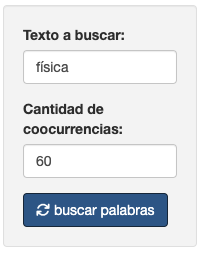
\includegraphics[width=0.25\linewidth]{images/05-desarrollo/2_ciclo/UI/prototipo_sidebar} 

}

\caption{Mock-Up de campos de entrada en la interfazde prototipo}\label{fig:sidebar}
\end{figure}

En lo relativo a los mapas de conocimiento, motivado a que visualizar gráficamente los resultados es una forma conveniente de ayudar a los usuarios a descubrir relaciones y patrones presentes en los textos que pueden estar ocultos (\protect\hyperlink{ref-li2018}{Li 2018}), en la Figura \ref{fig:mapacon}, se muestra la propuesta de representación de los mapas en el prototipo.

\begin{figure}

{\centering 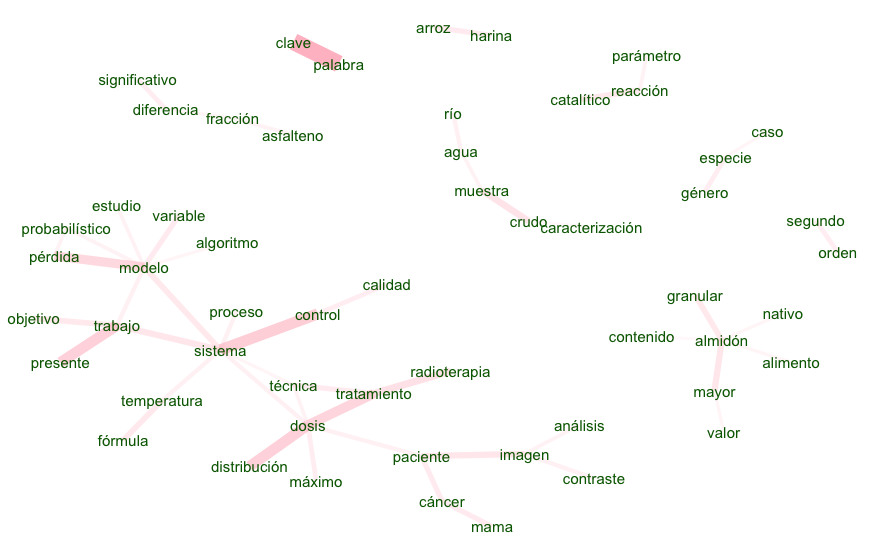
\includegraphics[width=0.7\linewidth]{images/05-desarrollo/2_ciclo/UI/mapcon} 

}

\caption{Representación mapas de conocimiento}\label{fig:mapacon}
\end{figure}

Otro punto a señalar es que, para implementar la búsqueda de texto se usará PostgreSQL V16, por lo cual en la fase de ``especulación'' se realizó el diseño del modelo ``entidad-relación'' que se ve en detalle en la Figura \ref{fig:entrel}.

\begin{figure}

{\centering 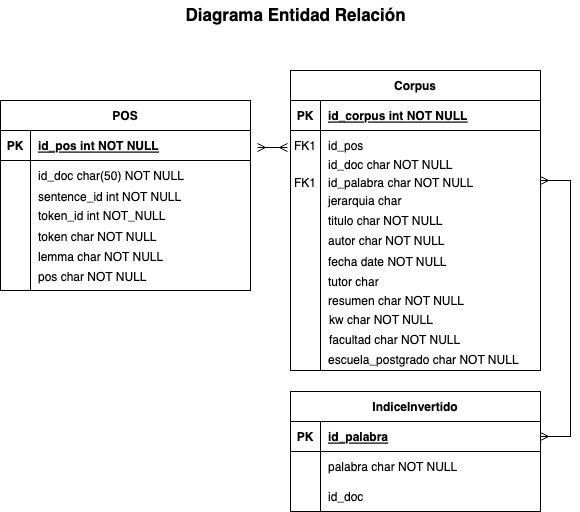
\includegraphics[width=0.6\linewidth]{images/05-desarrollo/2_ciclo/esquemas/diagrama_entidadrel} 

}

\caption{Modelo Entidad-Relación}\label{fig:entrel}
\end{figure}

En el modelo indicado, la entidad ``corpus'' se apoya en la tabla ``POS'' que contiene el detalle del etiquetado de la parte del discurso para cada palabra (token) presente en cada documento, mientras que la tabla ``indice invertido'' se destinará a almacenar la estructura que permite general la búsqueda de texto y básicamente almacena cada palabra que compone el vocabulario y el \emph{id} de los documentos donde aparece cada palabra.

Cabe destacar que, un factor determinante para la selección de PostgreSQL es el soporte que tiene para ejecutar procesos de ``búsqueda de texto completo (\emph{full text search})'' en el idioma español.

Igualmente se tiene que, el esquema de la arquitectura general de la aplicación, el cuál se implementará en el \emph{framework} Shiny, se representa en la Figura \ref{fig:esqshinyproto}.

\begin{figure}

{\centering 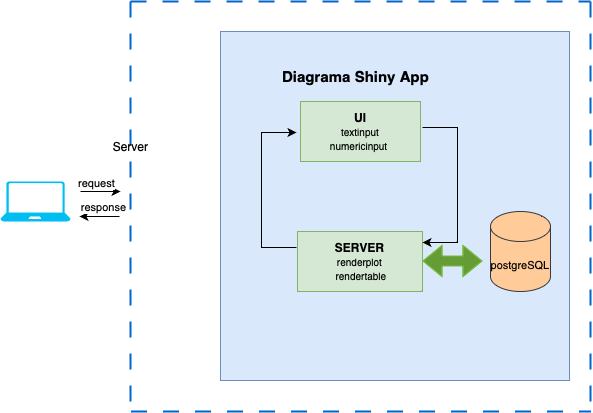
\includegraphics[width=0.5\linewidth]{images/05-desarrollo/2_ciclo/esquemas/shinyappproto} 

}

\caption{Esquema general de prototipo de la aplicación}\label{fig:esqshinyproto}
\end{figure}

\textbf{Colaboración}

La aplicación web que formará parte de prototipo, una vez que se tiene conformado el corpus anotado, se debe iniciar el poblado de la base de datos con las tres tablas que se mostraron en el diagrama de entidad relación propuesto en \ref{fig:entrel} .

A continuación se describen los procesos con los que se realizó el ``poblado\textbf{``} que sirve al prototipo.

\begin{enumerate}
\def\labelenumi{\arabic{enumi}.}
\item
  \textbf{Tabla Corpus}: con los datos del corpus anotado se conforma la tabla con los siguientes datos: jerarquía, título, nombre autor, fecha publicación, nombre de tutor, texto resumen, palabras claves, nombre de la facultad y nombre de la escuela-postgrado y el código único identificador de cada documento.

  \begin{enumerate}
  \def\labelenumii{\arabic{enumii}.}
  \item
    \textbf{Tabla ``indiceinvertido'':} mediante una extensión de PostrgreSQL V16.1 denominada ``\texttt{TS\_Vector}'', se crea una columna de nombre ``\texttt{document\_tokens}'', donde se almacena una estructura de datos de tipo ``\texttt{tsvector}'', que facilita al gestor de BD la búsqueda de texto completo. El \emph{script} siguiente hace el trabajo de crear el índice invertido mediante la función ``\texttt{to\_tsvector}'', para los datos del ``título'', ``palabras claves'', ``autor'' y del ``resumen''. En el mismo proceso se añaden pesos distintos (importancia para el criterio de reordenamiento de los resultados, según lo visto en \ref{ranking}, ``Re Ordenamiento'' ) a cada atributo mediante la función ``\texttt{setweight}''.

    \newpage

\begin{Shaded}
\begin{Highlighting}[]
\KeywordTok{ALTER} \KeywordTok{TABLE}\NormalTok{ Corpus }\KeywordTok{ADD} \KeywordTok{COLUMN}\NormalTok{ document\_tokens tsvector}
\KeywordTok{GENERATED}\NormalTok{ ALWAYS }\KeywordTok{AS}\NormalTok{ ((setweight(to\_tsvector(}\StringTok{\textquotesingle{}spanish\textquotesingle{}}\NormalTok{,}
                        \FunctionTok{coalesce}\NormalTok{(autor,}\StringTok{\textquotesingle{}\textquotesingle{}}\NormalTok{)),}\StringTok{\textquotesingle{}A\textquotesingle{}}\NormalTok{) }\OperatorTok{||}  
\NormalTok{                      setweight(to\_tsvector(}\StringTok{\textquotesingle{}spanish\textquotesingle{}}\NormalTok{,}
                        \FunctionTok{coalesce}\NormalTok{(titulo,}\StringTok{\textquotesingle{}\textquotesingle{}}\NormalTok{)),}\StringTok{\textquotesingle{}B\textquotesingle{}}\NormalTok{)}\OperatorTok{||}  
\NormalTok{                      setweight(to\_tsvector(}\StringTok{\textquotesingle{}spanish\textquotesingle{}}\NormalTok{,}
                        \FunctionTok{coalesce}\NormalTok{(kw,}\StringTok{\textquotesingle{}\textquotesingle{}}\NormalTok{)),}\StringTok{\textquotesingle{}C\textquotesingle{}}\NormalTok{)    }\OperatorTok{||}  
\NormalTok{                        setweight(to\_tsvector(}\StringTok{\textquotesingle{}spanish\textquotesingle{}}\NormalTok{,}
                        \FunctionTok{coalesce}\NormalTok{(resumen,}\StringTok{\textquotesingle{}\textquotesingle{}}\NormalTok{)),}\StringTok{\textquotesingle{}D\textquotesingle{}}\NormalTok{))) }
\NormalTok{                        STORED;}
\end{Highlighting}
\end{Shaded}

    En la Figura \ref{fig:doctok}, se puede ver parcialmente la estructura de datos de tipo ``\texttt{tsvector}'' que se genera para el texto ``Las planicies de inundación son sistemas asociados al margen de un río que están sujetas a pulsos estacionales de inundación y sequía. La desembocadura del Río Mapire constituye un sistema complejo de planicie de inundación, como resultado del aumento del nivel de agua en el río por un efecto de represamiento por el Río Orinoco durante la época lluviosa. El gradiente de inundación que se forma genera un estrés ambiental en el sistema suelo que depende de la duración y profundidad\ldots.'' .

    \begin{figure}

    {\centering 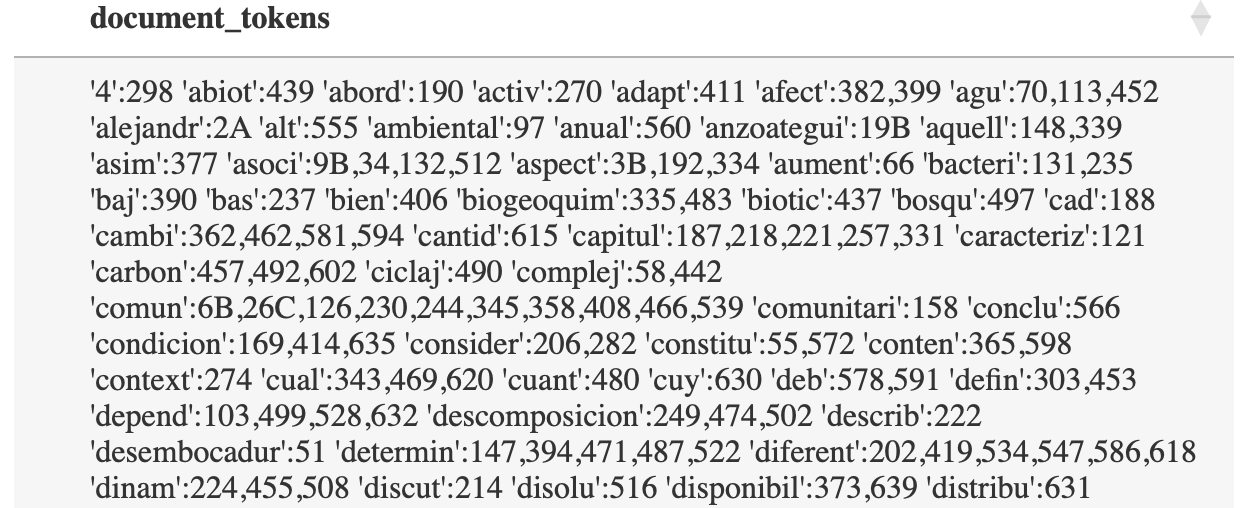
\includegraphics[width=0.85\linewidth]{images/05-desarrollo/2_ciclo/esquemas/doc_tokens} 

    }

    \caption{Estructura de datos índice invertido}\label{fig:doctok}
    \end{figure}

    La función ``\texttt{to\_tsvector}'' hace el \emph{parseo} de un documento a tokens y estos son modificados realizando el \emph{stemming} para extraer la raíz de la palabra, proceso que se revisó en \ref{steaming}, ``\emph{Stemming''}, lo cual ayuda a disminuir el espacio de búsqueda y a realizar la recuperación de textos de manera más eficiente. Para lograr ejecutar este proceso, es necesario dar el parámetro \texttt{spanish} a la función, para que sea sobre la base del idioma español que sea extraída la raíz.

    Igualmente, la posición de la palabra dentro del texto también queda registrada para así poder determinar en un \emph{query} de varias palabras la cercanía que tienen dentro del texto las palabras que son buscadas, dando una mayor relevancia a las que estén más cercanas.

    Otro aspecto a destacar es que ciertas palabras de uso común y frecuente, denominadas \emph{stopwords}, como: el, la, y, a, en, con, para; no son registradas, es decir que son omitidas así como los signos de puntuación, con lo cual un \emph{query} que contenga una \emph{stopword} o un signo de puntuación, no será buscada la coincidencia al no formar parte de la estructura de datos ``\texttt{tsvector}''.

    Para culminar el proceso de creación del índice invertido se debe ejecutar el comando ``\texttt{CREATE\ INDEX\ document\_weights\_idx\ ON\ Corpus\ USING\ GIN\ (document\_tokens);}'' que cierra el ciclo de la generación del índice y es lo que permite realizar los procesos de búsqueda en una forma más eficiente, disminuyendo los tiempos de respuesta, debiendo tener presente que la creación del índice puede incrementar entre un cincuenta y doscientos por ciento el espacio de almacenamiento al ser generado. Una de las bondades que adicionalmente brinda la función ``\texttt{TS\_VECTOR}'', es que al añadir nuevos documentos a la base de datos, el índice será actualizado automáticamente.
  \end{enumerate}
\item
  \textbf{Tabla ``POS'':} con los procesos que fueron ejecutados en \ref{iternlp}, ``Etiquetado de la Parte del Discurso'', se obtuvieron los datos que formarán parte de esta tabla, donde cada palabra que conforma el corpus pasa a ser una fila identificando el documento de origen, la oración dentro del documento donde se encuentra la palabra, el número de orden de aparición de la palabra, la palabra, su lema y la función gramatical asignada, idéntico a lo que se observó en la Figura \ref{fig:spacypi}.
\end{enumerate}

En cuanto a la aplicación web, mediante el \emph{framework} Shiny se implementó el prototipo con la codificación de dos componentes principales que son: la interfaz de usuario (ui) y el servidor (\emph{server}).

Es importante señalar que Shiny se sustenta en el uso de la ``programación reactiva'', lo que significa que ante cambios en los ``campos de entrada'' en la interfaz de usario (ui), los componentes relacionados se actualizan dinámicamente desde el componente ``server'' sin necesidad de recargar la página, permitiendo crear una experiencia al usuario fluida. Shiny utiliza conceptos como ``observadores'' y ``reactividad'' para mantener sincronizados los elementos de la ui con los datos subyacentes, que en el caso de prototipo son el texto del \emph{query}, el valor para establecer la cantidad de coocurrencias a representar en el ``mapa del conocimiento'' y el botón para ejecutar el \emph{query}.

\hfill\break
A nivel de la aplicación web, en la interfaz de usuario están estos tres componentes:

\begin{enumerate}
\def\labelenumi{\arabic{enumi}.}
\item
  \textbf{textInput}: corresponde a la casilla del \emph{query}.
\item
  \textbf{numericInput}: la cantidad de palabras que se van a mostrar en la representación de los mapas de conocimiento.
\item
  \textbf{actionBttn}: botón de acción para ejecutar el query.
\end{enumerate}

En el servidor de la aplicación, a nivel de generación de estructuras a ser representadas como resultados dispone de estos componentes:

\begin{enumerate}
\def\labelenumi{\arabic{enumi}.}
\item
  \textbf{dataTableOutput}: mediante la librería datatable (\protect\hyperlink{ref-DT}{Xie, Cheng, y Tan 2023a}) se genera una tabla con los resultados obtenidos donde se incluyen los atributos: ``fecha'',``títutlo'', ``autor'', ``resumen'', ``facultad'', ``escuela'', ``nombre tutor''.
\item
  \textbf{renderPlot}: con el uso de la librería ggraph (\protect\hyperlink{ref-ggraph}{Pedersen 2022a}) se crea un grafo que reproduce los mapas de conocimiento, representando las palabras mediante nodos y la coocurrencia implica la unión mediante arcos, y a mayor grosor en el arco, quiere decir que la cantidad de veces que se presenta la coocurrencia es mayor.
\end{enumerate}

En la Figura \ref{fig:prototipoapp}, se muestra la versión implementada del prototipo donde ante la búsqueda de la palabra ``física'' se recuperan los documentos que incluyen tal palabra y se generan los mapas de conocimiento.

\begin{figure}

{\centering 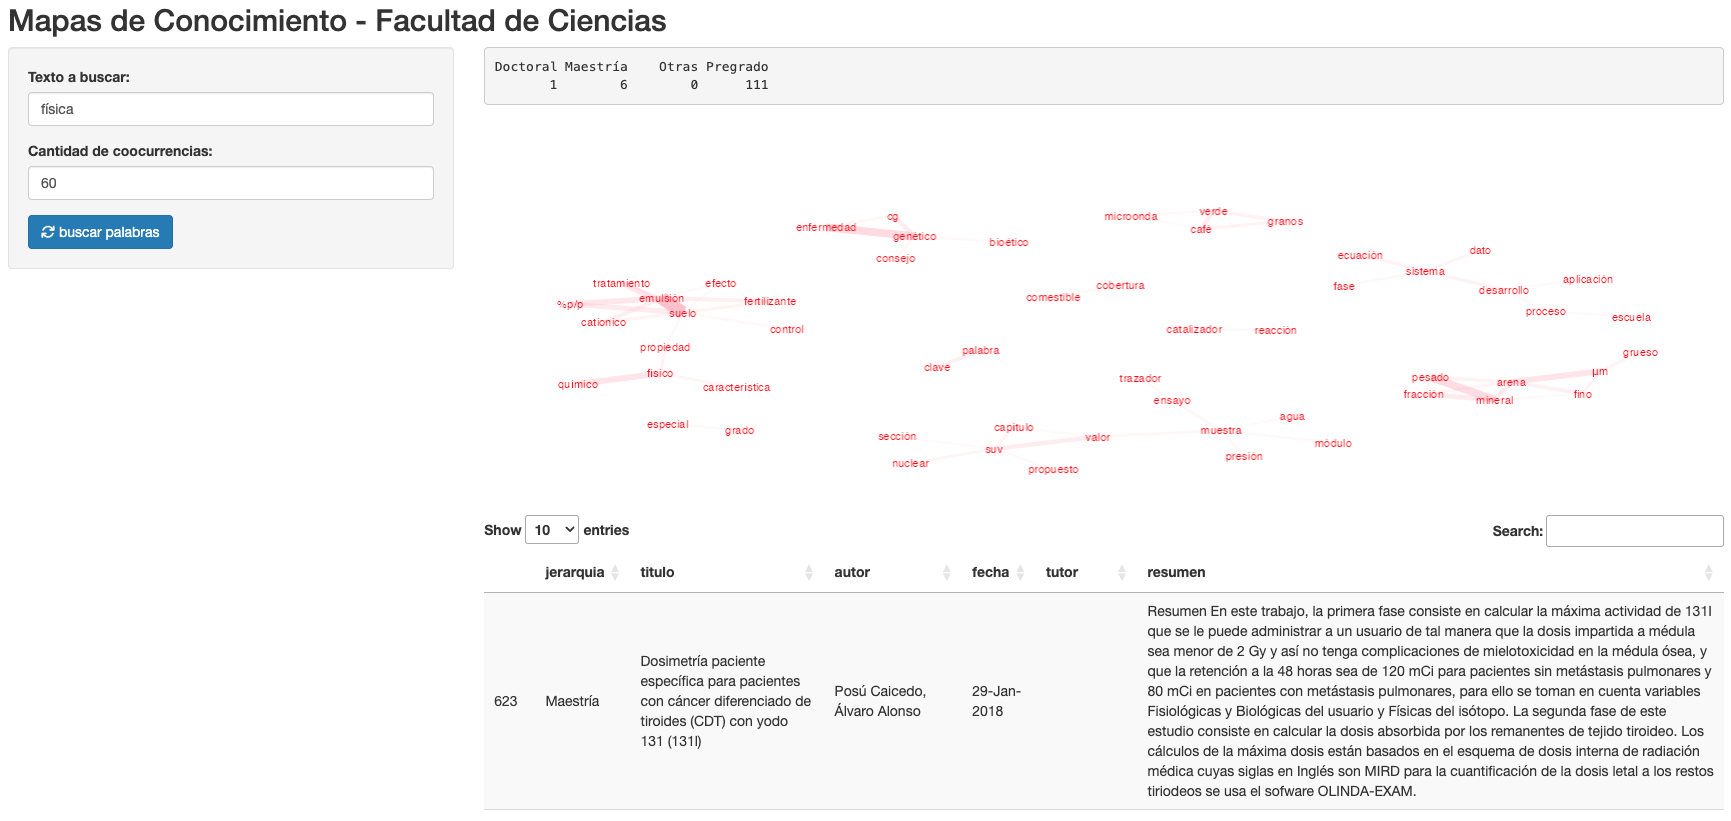
\includegraphics[width=0.8\linewidth]{images/05-desarrollo/2_ciclo/UI/prototipo_app} 

}

\caption{Resultado de búsqueda "física" en prototipo}\label{fig:prototipoapp}
\end{figure}

\textbf{Lógica de la Aplicación}

En el detalle que se expone en las siguientes líneas es necesario mencionar que Shiny, funciona a nivel de computo como monohilo (\emph{single-threaded}), por lo cual es estrictamente necesario que los pasos sean ejecutados secuencialmente según lo descrito.

\begin{enumerate}
\def\labelenumi{\arabic{enumi}.}
\item
  \textbf{Definición ``texto búsqueda'':} el usuario define el texto del \emph{query} y la cantidad de coocurrencias.
\item
  \textbf{Procesamiento \emph{query} texto:} cuando el servidor recibe el texto para generar el \emph{query}, este es procesado con la sintaxis del siguiente código:

\begin{Shaded}
\begin{Highlighting}[]
\OtherTok{"select titulo, id\_doc, facultad, jerarquia ,fecha,}
\NormalTok{  autor, kw, resumen, nombre, tutor }\KeywordTok{from}\NormalTok{ Corpus }\KeywordTok{where}
\NormalTok{  document\_tokens @@ websearch\_to\_tsquery(}\StringTok{\textquotesingle{}spanish\textquotesingle{}}\NormalTok{,}
    \StringTok{\textquotesingle{}texto a buscar\textquotesingle{}}\NormalTok{) }
  \KeywordTok{order} \KeywordTok{by}\NormalTok{ ts\_rank\_cd (document\_tokens,}
\NormalTok{    websearch\_to\_tsquery(}\StringTok{\textquotesingle{}spanish\textquotesingle{}}\NormalTok{,}\StringTok{\textquotesingle{}texto a buscar\textquotesingle{}}\NormalTok{)) }\KeywordTok{desc}
\end{Highlighting}
\end{Shaded}

  Lo relevante es apreciar que el texto del \emph{query}, mediante la función ``\texttt{websearch\_to\_tsquery}'', es sometido a un \emph{parseo} que lo convierte a la estructura de datos ``\texttt{tsvector}'', revisada anteriormente, y así la hace compatible con el contenido de la columna ``\texttt{document\_tokens}''. El operador de coincidencia ``\texttt{@@}'' es el que determina si el texto del ``\texttt{tsquery}'' coincide con los distintos textos registrados en el ``\texttt{tsvector}''. Si la frase del query, p.~ej.''física química'', que incluye dos palabras, el operador lógico que se intercala entre cada palabra es el ``y (AND)'', no obstante, la propia función ``\texttt{websearch\_to\_tsquery}'' permite que se defina que pueda ser el operador ``o (OR)'', por ejemplo si se escribe ``física OR química'' \footnote{Otros operadores que se pueden usar en esta función son: ``!'' para excluir un término, ``\textless-\textgreater{}'' para indicar que las palabras deben aparecer una seguida de otra. En la documentación oficial de PostgreSQL disponible en el enlace \url{https://www.postgresql.org/docs/current/textsearch-controls.html} se encuentra más información sobre los operadores que se pueden aplicar en los procesos de búsqueda.}.

  También incluye la función ``\texttt{order\ by\ ts\_rank\_cd}'' la cual es una implementación del método ``\emph{cover density}~\emph{ranking}''~que fue introducido en la investigación de (\protect\hyperlink{ref-clarke2000}{Clarke, Cormack, y Tudhope 2000}), donde la relevancia se determina mediante la proximidad y coocurrencia de las palabras que conforman el \emph{query} dentro de cada documento del corpus ejecutando el reordenamiento, según lo visto en \ref{ranking}, ``Re Ordenamiento'',teniendo como base los criterios de peso que habían sido definidos al crear el ``\texttt{tsvector}'' y también toma en cuenta la proximidad que puedan tener las distintas palabras que componen el query. Es conveniente citar la documentación de PostgreSQL relativa a esta función ``\ldots{}\emph{es decir, consideran la frecuencia con la que los términos de la consulta aparecen en el documento, la proximidad de los términos en el documento y la importancia de la parte del documento en la que aparecen. Sin embargo, el concepto de relevancia es vago y muy específico de cada aplicación. Diferentes aplicaciones pueden requerir información adicional para la clasificación, por ejemplo, la hora de modificación del documento}''.\\
\item
  \textbf{Query datos mapas de conocimiento:} con la lista de ``id\_docs'', que fue obtenida en el paso anterior, se ejecuta un segundo \emph{query} sobre la tabla ``POS'', se seleccionan las filas que tienen la lista de ``id\_docs'' y aquellas en las cuales las palabras (\emph{tokens}) cumplan con la condición de ser sustantivos y adjetivos, obteniendo la tabla filtrada con ``doc\_id'', ``token\_id'', ``sentence\_id'', ``pos'', ``lemma''.

  Contar en esta tabla con el ``doc\_id'', ``token\_id'' y el ``sentence\_id'', sirve para determinar el nivel de representación de las coocurrencias a modo de granularidad, permitiendo que posteriormente el resultado pueda ser representado con palabras que coocurren: a) una seguida de otra, b) dentro de la misma oración, o, c) dentro del mismo texto resumen.
\item
  \textbf{Generación de estructura mapas de conocimiento-coocurrencia:} los datos obtenidos en el paso previo se les aplica la función \texttt{coocurrence} de la librería UDPipe (\protect\hyperlink{ref-udpipe-4}{Wijffels 2023a}) que convierte los datos en una tabla de coocurrencias, donde se puede ajustar la granularidad revisada en el paso anterior.
\item
  \textbf{Render resultados:} el servidor hace el render del ``\texttt{dataTableOutput}'' y del ``\texttt{renderPlot}'' mencionados.
\end{enumerate}

\textbf{Aprender}

En la fase de aprendizaje se pudo detectar que es conveniente hacer distintas representaciones de los mapas de conocimiento con distintas granularidades y que incorporar interactividad a la representación puede constituir una herramienta de filtrado adicional para inspeccionar el corpus. En el ciclo \ref{desarrollociclos4}, ``Ciclo de Integración de Componentes del Software'', será abordado en detalle la propuesta final que se implementó en este particular.

Igualmente, se constató la necesidad de mejorar los niveles de reproducibilidad para realizar la implementación del sistema, mediante configuraciones que puedan ser independientes del sistema operativo y demás dependencias que estén preinstaladas en el \emph{host}, lo que llevó a realizar el diseño de la aplicación y sus componentes, mediante el uso de contenedores orquestados, lo cual se expondrá en \ref{desarrollociclos4}, ``Ciclo Integración de Componentes del Software''.

Al crear el índice invertido se pudo apreciar que el peso de la tabla con los datos del corpus se incrementó en aproximadamente un 40\%, no obstante, por ser un conjunto de datos relativamente pequeño, esto no representa un mayor problema, pero sí se debe tener en cuenta en caso de que el sistema diese soporte a un corpus mucho mayor.

Otro proceso de aprendizaje de este ciclo fue, hacer los ajustes a la función de reordenamiento, según la relevancia, donde se estableció la siguiente jerarquía:

\begin{enumerate}
\def\labelenumi{\arabic{enumi}.}
\item
  Autor.
\item
  Título.
\item
  Palabras clave.
\item
  Texto resumen.
\end{enumerate}

Lo que quiere decir que si ante un texto de una búsqueda, en los documentos que conforman el corpus, las palabras de \emph{query} presentan coincidencia en el título, la función de relevancia le otorgará mayor peso a ese documento por sobre otro que pueda tener la misma coincidencia de aparición, pero en el texto resumen. Este ejemplo aplica para el resto de las combinaciones posibles.

Adicionalmente, realizar el etiquetado de las partes del discurso, previamente a realizar la selección de los textos que serán representados mediante mapas de conocimiento, representa una mejora en los tiempos que tarda el prototipo en realizar el render, lo cual refuerza la necesidad de contar con un sistema gestor de base de datos que pueda tener indexadas las distintas tablas que conforman el SCSU.

\hypertarget{objetivos-alcanzados-1}{%
\subsubsection{Objetivos Alcanzados:}\label{objetivos-alcanzados-1}}

\begin{enumerate}
\def\labelenumi{\arabic{enumi}.}
\item
  Implementar un buscador de texto sobre un subconjunto del corpus.
\item
  Hacer las pruebas de integración entre la base de datos con la aplicación web.
\item
  Contar con almacenamiento persistente para los datos.
\item
  Generar recomendaciones de documentos que sean similares a una determinada investigación, acorde a \ref{objeespe}, ``Objetivo Específico - 4''.
\end{enumerate}

\newpage

\hypertarget{desarrollociclos4}{%
\subsection{Ciclo Integración de Componentes del Software}\label{desarrollociclos4}}

En este ciclo, tomando de insumo los aprendizajes obtenidos en los ciclos anteriores, se hace la integración de los distintos componentes y se realizan las modificaciones que permiten obtener la primera versión completa y funcional del SCSU, que puede ser puesto en producción.

\textbf{Especulación}

Usando las técnicas y métodos aplicados en ciclos anteriores e integrando los aprendizajes obtenidos, se puede implementar el SCSU. Concretamente se tendrá como insumo en este ciclo lo revisado y obtenido en:

\begin{enumerate}
\def\labelenumi{\arabic{enumi}.}
\item
  Usar la arquitectura ``modelo-vista-contralador'' revisada en \ref{desarrolloarquitectura}, ``Arquitectura de la Solución''.
\item
  Usar el corpus conformado en \ref{desarrollociclos1}, ``Conformación del Conjunto de Datos''.
\item
  Usar los documentos clasificados que se obtuvieron en \ref{asignacion}, ``Clasificación de Documentos''.
\item
  Usar el método ``Búsqueda de textos'' revisado en \ref{desarrollociclos3}, ``Prototipo del SCSU''.
\item
  Usar el método de representación de mapas de conocimiento revisado en \ref{fig:mapacon}, ``Prototipo del SCSU''.
\item
  Usar el método para realizar la generación de ``recomendaciones'' revisado en \ref{imrecomendacion}, ``Recomendación de Documentos''.
\end{enumerate}

En el proceso de especulación de este ciclo se aplicaron los métodos de la ``ingeniería de software'' necesarios para implementar el SCSU estableciendo formalmente los requerimientos funcionales y no funcionales, los diagramas y tablas de casos de uso, el modelo entidad-relación y demás aspectos necesarios, para posteriormente en la fase de colaboración realizar la implementación del sistema.

\newpage

\textbf{Requerimientos Funcionales del SCSU:}

\begin{enumerate}
\def\labelenumi{\arabic{enumi}.}
\tightlist
\item
  \textbf{Interactividad:}
\end{enumerate}

\begin{itemize}
\item
  \textbf{Descripción}

  La aplicación web debe ser altamente interactiva permitiendo al usuario de una manera fluida y receptiva interactuar con la interfaz para realizar búsquedas, explorar resultados y utilizar funcionalidades como filtros e inspección de mapas de conocimiento.
\item
  \textbf{Criterios de Aceptación}

  \begin{itemize}
  \tightlist
  \item
    La interfaz de usuario debe responder de manera rápida y efeciciente a las interacciones del usuario.
  \end{itemize}
\end{itemize}

\begin{enumerate}
\def\labelenumi{\arabic{enumi}.}
\setcounter{enumi}{1}
\tightlist
\item
  \textbf{Búsqueda de Contenido:}
\end{enumerate}

\begin{itemize}
\item
  \textbf{Descripción}

  El sistema debe permitir a los usuarios realizar búsquedas de contenido utilizando palabras clave o frases. La búsqueda debe ser insensible a mayúsculas y minúsculas, y devolver resultados en función a las palabras clave ingresadas.

  \textbf{Criterios de Aceptación}

  \begin{itemize}
  \tightlist
  \item
    El sistema debe proporcionar una interfaz de usuario intuitiva para la entrada de términos de búsqueda.
  \item
    Los resultados de la búsqueda deben mostrar: títulos, autores, fecha elaboración, palabras clave, facultad, nombre tutor, resúmenes.
  \item
    La búsqueda debe ser eficiente, respondiendo en un tiempo razonable.
  \item
    Se debe permitir a los usuarios hacer clic en un resultado para obtener más detalles sobre una investigación.
  \end{itemize}
\end{itemize}

\begin{enumerate}
\def\labelenumi{\arabic{enumi}.}
\setcounter{enumi}{2}
\tightlist
\item
  \textbf{Filtrado de Búsquedas:}
\end{enumerate}

\begin{itemize}
\item
  \textbf{Descripción}

  El sistema debe permitir a los usuarios aplicar filtros avanzados a los resultados de búsqueda para refinar y limitar la información recuperada. Los filtros pueden incluir fechas, jerarquía (nivel académico), facultad, escuela-postgrado.

  \newpage
\item
  \textbf{Criterios de Aceptación}

  \begin{itemize}
  \item
    Los filtros deben ser fácilmente accesibles y configurables.
  \item
    Las opciones de criterios de búsqueda deben actualizarse dinámicamente al aplicar los filtros.
  \item
    Debe ser posible combinar múltiples filtros para refinar aún más la búsqueda.
  \end{itemize}
\end{itemize}

\begin{enumerate}
\def\labelenumi{\arabic{enumi}.}
\setcounter{enumi}{3}
\tightlist
\item
  \textbf{Generar Mapas de Conocimiento:}
\end{enumerate}

\begin{itemize}
\item
  \textbf{Descripción}

  El sistema debe tener la capacidad de generar mapas de conocimiento con la información recuperada. Estos mapas deben representar de manera clara las relaciones y conexiones entre los conceptos dentro de la información mediante una estructura de grafos.
\item
  \textbf{Criterios de Aceptación}

  \begin{itemize}
  \item
    La generación de mapas de conocimiento debe ser automática y basarse en la estructura y contenido de los documentos recuperados.
  \item
    Los mapas deben ser interactivos, permitiendo a los usuarios explorar y comprender las relaciones entre los conceptos.
  \item
    Deben existir opciones para ajustar la complejidad y el nivel de detalle de los mapas.
  \end{itemize}
\end{itemize}

\begin{enumerate}
\def\labelenumi{\arabic{enumi}.}
\setcounter{enumi}{4}
\tightlist
\item
  \textbf{Jerarquizar los Documentos Recuperados:}
\end{enumerate}

\begin{itemize}
\item
  \textbf{Descripción}

  El sistema debe asignar un \emph{ranking} a los documentos recuperados en función de su relevancia con respecto a la consulta realizada. La clasificación debe ser transparente y basada en algoritmos que consideren diversos factores como la frecuencia y proximidad de términos clave.
\item
  \textbf{Criterios de Aceptación}

  \begin{itemize}
  \item
    Aplicar algoritmo para reordamiento y evaluar las métricas de desempeño.
  \item
    Se debe proporcionar una opción para ordenar los resultados de búsqueda según diferentes criterios, como relevancia o fecha.
  \end{itemize}
\end{itemize}

\begin{enumerate}
\def\labelenumi{\arabic{enumi}.}
\setcounter{enumi}{5}
\tightlist
\item
  \textbf{Generar Recomendaciones:}
\end{enumerate}

\begin{itemize}
\item
  \textbf{Descripción}

  El sistema debe ofrecer recomendaciones de contenido relevante basadas en similitud que tenga un documento con los otros que conforman el corpus.
\item
  \textbf{Criterios de Aceptación}

  \begin{itemize}
  \tightlist
  \item
    Las recomendaciones deben ser presentadas de manera clara indicando el título de la investigación recomendada con un vínculo al trabajo presentado.
  \end{itemize}
\end{itemize}

\begin{enumerate}
\def\labelenumi{\arabic{enumi}.}
\setcounter{enumi}{6}
\tightlist
\item
  \textbf{Actualizar Periódicamente las Investigaciones:}
\end{enumerate}

\begin{itemize}
\item
  \textbf{Descripción}

  El sistema debe realizar actualizaciones periódicas de la información almacenada, garantizando que los resultados de búsqueda sean siempre actuales y reflejen los documentos incorporados a Saber U.C.V. y que estos sean clasificados por área de conocimiento.
\item
  \textbf{Criterios de Aceptación}

  \begin{itemize}
  \item
    Deben establecerse intervalos regulares de actualización de la base de datos.
  \item
    Las actualizaciones no deben afectar negativamente el rendimiento del sistema durante las operaciones normales.
  \end{itemize}
\end{itemize}

\begin{enumerate}
\def\labelenumi{\arabic{enumi}.}
\setcounter{enumi}{7}
\tightlist
\item
  \textbf{Cuadros de Ayuda (\emph{Tooltips}):}
\end{enumerate}

\begin{itemize}
\item
  \textbf{Descripción}

  El sistema debe proporcionar cuadros de ayuda (\emph{tooltips}) contextuales para guiar a los usuarios durante la interacción con la interfaz. Estos cuadros deben explicar términos técnicos, funciones específicas y proporcionar orientación sobre el uso eficaz del sistema.
\item
  \textbf{Criterios de Aceptación}

  \begin{itemize}
  \item
    Deben existir cuadros de ayuda accesibles en puntos clave de la interfaz de usuario.
  \item
    Los \emph{tooltips} deben ser informativos y fácilmente comprensible su contenido.
  \end{itemize}
\end{itemize}

\begin{enumerate}
\def\labelenumi{\arabic{enumi}.}
\setcounter{enumi}{8}
\tightlist
\item
  \textbf{Accesibilidad Web:}
\end{enumerate}

\begin{itemize}
\item
  \textbf{Descripción}

  El acceso a la aplicación se debe realizar mediante un navegadores web desde cualquier sitio.
\item
  \textbf{Criterios de Aceptación}

  \begin{itemize}
  \tightlist
  \item
    Se debe garantizar la compatibilidad con los navegadores web más utilizados, como Chrome, Firefox, Safari y Edge.
  \end{itemize}
\end{itemize}

\textbf{Requerimientos No Funcionales del SCSU}

\begin{enumerate}
\def\labelenumi{\arabic{enumi}.}
\tightlist
\item
  \textbf{Rendimiento del Sistema:}
\end{enumerate}

\begin{itemize}
\item
  \textbf{Descripción}

  El sistema debe ser capaz de manejar eficientemente los volúmenes de datos proporcionando tiempos de respuesta rápidos. El rendimiento del sistema debe optimizarse para garantizar una experiencia de usuario fluida y satisfactoria, independientemente de la complejidad de las consultas o la cantidad de usuarios concurrentes.
\item
  \textbf{Criterios de Aceptación}

  \begin{itemize}
  \item
    El tiempo de respuesta promedio para una consulta estándar no debe superar un segundo.

    \newpage
  \end{itemize}
\end{itemize}

\begin{enumerate}
\def\labelenumi{\arabic{enumi}.}
\setcounter{enumi}{1}
\tightlist
\item
  \textbf{Utilización de Componentes \emph{open source:}}
\end{enumerate}

\begin{itemize}
\item
  \textbf{Descripción}

  El SCSU debe utilizar componentes de software (bibliotecas, frameworks y herramientas) que estén bajo licencias \emph{open source}.
\item
  \textbf{Criterios de Aceptación}

  \begin{itemize}
  \tightlist
  \item
    Se debe realizar una evaluación de la licencia de los componentes utilizados para garantizar su compatibilidad con el modelo de desarrollo y distribución del proyecto.
  \end{itemize}
\end{itemize}

\begin{enumerate}
\def\labelenumi{\arabic{enumi}.}
\setcounter{enumi}{2}
\tightlist
\item
  \textbf{Reproducibilidad del SCSU:}
\end{enumerate}

\begin{itemize}
\item
  \textbf{Descripción}

  El sistema debe ser reproducible, lo que significa que la construcción, implementación y ejecución del software deben proporcionar resultados consistentes en diferentes entornos y momentos, siguiendo prácticas y estándares que faciliten la reproducibilidad del proceso de desarrollo.
\item
  \textbf{Criterios de Aceptación}

  \begin{itemize}
  \item
    Todas las dependencias externas, incluyendo bibliotecas y componentes \emph{open source}, deben estar claramente especificadas y gestionadas.
  \item
    La aplicación debe ser capaz de ejecutarse correctamente en diferentes sistemas operativos y configuraciones de infraestructura.
  \end{itemize}
\end{itemize}

\begin{enumerate}
\def\labelenumi{\arabic{enumi}.}
\setcounter{enumi}{3}
\tightlist
\item
  \textbf{Preprocesamientos:}
\end{enumerate}

\begin{itemize}
\item
  \textbf{Descripción}

  El sistema, bien sea al momento de conformar la base de datos o al realizar actualizaciones, en la mayor medida posible debe ejecutar el preprocesamiento de los textos (PLN-POS, remoción \emph{stopwords}, índice invertido, etc.) para minimizar los cómputos al momento de la demanda de recursos cuando el usuario realiza las búsquedas.

  \newpage
\item
  \textbf{Criterios de Aceptación}

  \begin{itemize}
  \tightlist
  \item
    El sistema debe realizar el preprocesamiento de textos de manera eficiente durante la construcción inicial de la base de datos y las actualizaciones periódicas.
  \end{itemize}
\end{itemize}

\begin{enumerate}
\def\labelenumi{\arabic{enumi}.}
\setcounter{enumi}{4}
\tightlist
\item
  \textbf{Modularidad del Sistema:}
\end{enumerate}

\begin{itemize}
\item
  \textbf{Descripción}

  El sistema debe ser modular, dividiendo sus componentes en piezas simples que utilizan contenedores. Estos componentes deben estar orquestados de manera eficiente, permitiendo el intercambio, la asignación de recursos y la modificación de módulos individuales con un impacto mínimo en el resto del sistema.
\item
  \textbf{Criterios de Aceptación}

  \begin{itemize}
  \item
    Los componentes del sistema deben estar encapsulados en contenedores, facilitando su independencia y despliegue consistente.
  \item
    Los componentes del sistema deben estar orquestados de manera eficiente, permitiendo una coordinación efectiva entre ellos y permitiendo la definición de asignación de recursos.
  \item
    Los componentes deben ser intercambiables y modificables de manera independiente, fomentando la flexibilidad y la evolución del sistema a lo largo del tiempo.
  \end{itemize}
\end{itemize}

\begin{enumerate}
\def\labelenumi{\arabic{enumi}.}
\setcounter{enumi}{5}
\tightlist
\item
  \textbf{Mantenibilidad del Sistema:}
\end{enumerate}

\begin{itemize}
\item
  \textbf{Descripción}

  El sistema debe ser diseñado de manera que permita la realización periódica de mantenimiento sin degradar el rendimiento ni la operatividad del sistema.
\item
  \textbf{Criterios de Aceptación}

  \begin{itemize}
  \item
    La realización de mantenimiento no debe causar una degradación significativa en el rendimiento del sistema garantizando la continuidad operativa.
  \item
    La realización del mantenimiento debe definirse con carácter periódico en la configuración.
  \end{itemize}
\end{itemize}

\textbf{Diagramas de Caso de Uso}

El SCSU cuenta con los casos de uso que se observan en las figuras \ref{fig:uc1}, \ref{fig:uc12}, \ref{fig:uc2}, \ref{fig:uc3}, \ref{fig:uc31}, \ref{fig:uc4} ; seguido de las tablas \ref{tab:tablauc1} ,\ref{tab:tablauc11} , \ref{tab:tablauc2}, \ref{tab:tablauc3}, \ref{tab:tablauc321}, \ref{tab:tablauc322}, \ref{tab:tablauc4}, que contienen la descripción de cada caso.

\begin{figure}

{\centering 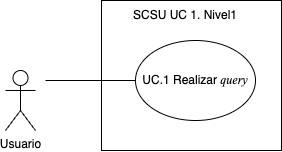
\includegraphics[width=0.4\linewidth]{images/05-desarrollo/4_ciclo/UC/SCSU_UC1_nivel1} 

}

\caption{SCSU: Diagrama de casos de uso 1, nivel 1.}\label{fig:uc1}
\end{figure}

\begin{figure}

{\centering 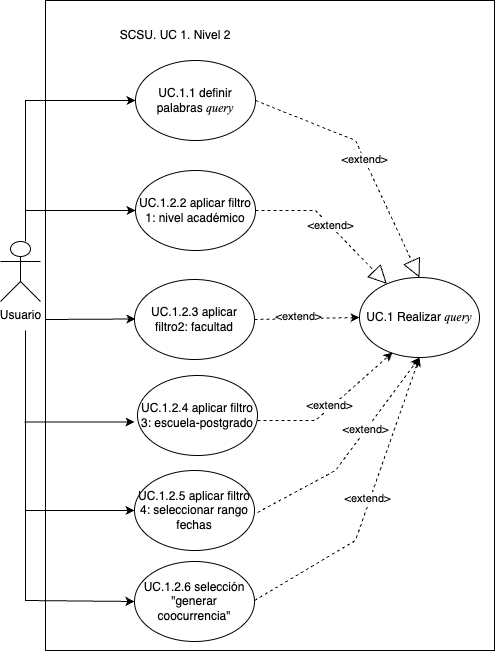
\includegraphics[width=0.5\linewidth]{images/05-desarrollo/4_ciclo/UC/SCSU_UC1_nivel2} 

}

\caption{SCSU: Diagrama de casos de uso 1, nivel 1.}\label{fig:uc12}
\end{figure}

\begin{figure}

{\centering 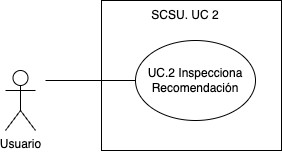
\includegraphics[width=0.4\linewidth]{images/05-desarrollo/4_ciclo/UC/SCSU_UC2_nivel1} 

}

\caption{SCSU: Diagrama de casos de uso 2.}\label{fig:uc2}
\end{figure}

\begin{figure}

{\centering 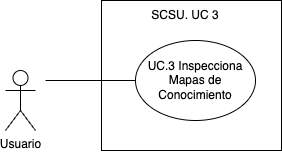
\includegraphics[width=0.4\linewidth]{images/05-desarrollo/4_ciclo/UC/SCSU_UC3_nivel1} 

}

\caption{SCSU: Diagrama de casos de uso 3, nivel 1}\label{fig:uc3}
\end{figure}

\begin{figure}

{\centering 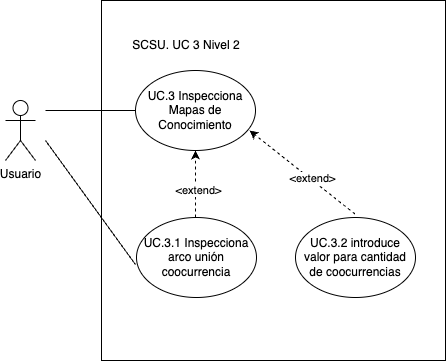
\includegraphics[width=0.5\linewidth]{images/05-desarrollo/4_ciclo/UC/SCSU_UC3_nivel2} 

}

\caption{SCSU: Diagrama de casos de uso 3, nivel 2.}\label{fig:uc31}
\end{figure}

\begin{figure}

{\centering 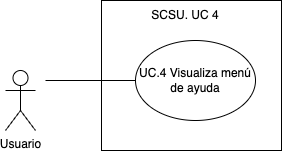
\includegraphics[width=0.4\linewidth]{images/05-desarrollo/4_ciclo/UC/SCSU_UC4} 

}

\caption{SCSU: Diagrama de casos de uso 4.}\label{fig:uc4}
\end{figure}

\newpage

\newpage

\global\setlength{\Oldarrayrulewidth}{\arrayrulewidth}

\global\setlength{\Oldtabcolsep}{\tabcolsep}

\setlength{\tabcolsep}{0pt}

\renewcommand*{\arraystretch}{1.5}



\providecommand{\ascline}[3]{\noalign{\global\arrayrulewidth #1}\arrayrulecolor[HTML]{#2}\cline{#3}}

\begin{longtable}[c]{|p{1.00in}|p{6.00in}}

\caption{SCSU\ UC.1.}\label{tab:tablauc1}\\

\hhline{>{\arrayrulecolor[HTML]{666666}\global\arrayrulewidth=0.75pt}->{\arrayrulecolor[HTML]{666666}\global\arrayrulewidth=0.75pt}-}

\multicolumn{1}{!{\color[HTML]{666666}\vrule width 0.75pt}>{\cellcolor[HTML]{C2C2C2}\raggedright}m{\dimexpr 1in+0\tabcolsep}}{\textcolor[HTML]{000000}{\fontsize{10}{10}\selectfont{\global\setmainfont{Helvetica}{Nombre}}}} & \multicolumn{1}{!{\color[HTML]{666666}\vrule width 0.75pt}>{\raggedright}m{\dimexpr 6in+0\tabcolsep}!{\color[HTML]{666666}\vrule width 0.75pt}}{\textcolor[HTML]{000000}{\fontsize{10}{10}\selectfont{\global\setmainfont{Helvetica}{UC.1:\ Realizar\ proceso\ de\ recuperación\ de\ información\ (query)}}}} \\

\noalign{\global\arrayrulewidth 0.75pt}\arrayrulecolor[HTML]{666666}

\hhline{|>{\arrayrulecolor[HTML]{666666}\global\arrayrulewidth=0.75pt}-|>{\arrayrulecolor[HTML]{666666}\global\arrayrulewidth=0.75pt}-}



\multicolumn{1}{!{\color[HTML]{666666}\vrule width 0.75pt}>{\cellcolor[HTML]{C2C2C2}\raggedright}m{\dimexpr 1in+0\tabcolsep}}{\textcolor[HTML]{000000}{\fontsize{10}{10}\selectfont{\global\setmainfont{Helvetica}{Descripción}}}} & \multicolumn{1}{!{\color[HTML]{666666}\vrule width 0.75pt}>{\raggedright}m{\dimexpr 6in+0\tabcolsep}!{\color[HTML]{666666}\vrule width 0.75pt}}{\textcolor[HTML]{000000}{\fontsize{10}{10}\selectfont{\global\setmainfont{Helvetica}{El\ usuario\ realiza\ búsquedas\ sobre\ los\ textos\ que\ conforman\ el\ corpus}}}} \\

\noalign{\global\arrayrulewidth 0.75pt}\arrayrulecolor[HTML]{666666}

\hhline{|>{\arrayrulecolor[HTML]{666666}\global\arrayrulewidth=0.75pt}-|>{\arrayrulecolor[HTML]{666666}\global\arrayrulewidth=0.75pt}-}



\multicolumn{1}{!{\color[HTML]{666666}\vrule width 0.75pt}>{\cellcolor[HTML]{C2C2C2}\raggedright}m{\dimexpr 1in+0\tabcolsep}}{\textcolor[HTML]{000000}{\fontsize{10}{10}\selectfont{\global\setmainfont{Helvetica}{Actor}}}} & \multicolumn{1}{!{\color[HTML]{666666}\vrule width 0.75pt}>{\raggedright}m{\dimexpr 6in+0\tabcolsep}!{\color[HTML]{666666}\vrule width 0.75pt}}{\textcolor[HTML]{000000}{\fontsize{10}{10}\selectfont{\global\setmainfont{Helvetica}{Usuario}}}} \\

\noalign{\global\arrayrulewidth 0.75pt}\arrayrulecolor[HTML]{666666}

\hhline{|>{\arrayrulecolor[HTML]{666666}\global\arrayrulewidth=0.75pt}-|>{\arrayrulecolor[HTML]{666666}\global\arrayrulewidth=0.75pt}-}



\multicolumn{2}{!{\color[HTML]{666666}\vrule width 0.75pt}>{\cellcolor[HTML]{8F8F8F}\centering}m{\dimexpr 7in+2\tabcolsep+0.75pt}!{\color[HTML]{666666}\vrule width 0.75pt}}{\textcolor[HTML]{000000}{\fontsize{10}{10}\selectfont{\global\setmainfont{Helvetica}{Flujo\ de\ Eventos}}}} \\

\noalign{\global\arrayrulewidth 0.75pt}\arrayrulecolor[HTML]{666666}

\hhline{|>{\arrayrulecolor[HTML]{666666}\global\arrayrulewidth=0.75pt}-|>{\arrayrulecolor[HTML]{666666}\global\arrayrulewidth=0.75pt}-}



\multicolumn{2}{!{\color[HTML]{666666}\vrule width 0.75pt}>{\cellcolor[HTML]{A3A3A3}\raggedright}m{\dimexpr 7in+2\tabcolsep+0.75pt}!{\color[HTML]{666666}\vrule width 0.75pt}}{\textcolor[HTML]{000000}{\fontsize{10}{10}\selectfont{\global\setmainfont{Helvetica}{Flujo\ Básico}}}} \\

\noalign{\global\arrayrulewidth 0.75pt}\arrayrulecolor[HTML]{666666}

\hhline{|>{\arrayrulecolor[HTML]{666666}\global\arrayrulewidth=0.75pt}-|>{\arrayrulecolor[HTML]{666666}\global\arrayrulewidth=0.75pt}-}



\multicolumn{2}{!{\color[HTML]{666666}\vrule width 0.75pt}>{\raggedright}m{\dimexpr 7in+2\tabcolsep+0.75pt}!{\color[HTML]{666666}\vrule width 0.75pt}}{\textcolor[HTML]{000000}{\fontsize{10}{10}\selectfont{\global\setmainfont{Helvetica}{El\ caso\ de\ uso\ inicia\ cuando\ el\ usuario\ ingresa\ a\ la\ aplicación:\ }}}\textcolor[HTML]{000000}{\fontsize{10}{10}\selectfont{\global\setmainfont{Helvetica}{\linebreak }}}\textcolor[HTML]{000000}{\fontsize{10}{10}\selectfont{\global\setmainfont{Helvetica}{\ 1)\ Introduce\ el\ texto\ a\ buscar.\ }}}\textcolor[HTML]{000000}{\fontsize{10}{10}\selectfont{\global\setmainfont{Helvetica}{\linebreak }}}\textcolor[HTML]{000000}{\fontsize{10}{10}\selectfont{\global\setmainfont{Helvetica}{\ 2)\ El\ usuario\ hace\ clic\ en\ "búsqueda"\ }}}\textcolor[HTML]{000000}{\fontsize{10}{10}\selectfont{\global\setmainfont{Helvetica}{\linebreak }}}\textcolor[HTML]{000000}{\fontsize{10}{10}\selectfont{\global\setmainfont{Helvetica}{\ 4)\ El\ SCSU\ presenta\ los\ resultados\ obtenidos\ }}}\textcolor[HTML]{000000}{\fontsize{10}{10}\selectfont{\global\setmainfont{Helvetica}{\linebreak }}}\textcolor[HTML]{000000}{\fontsize{10}{10}\selectfont{\global\setmainfont{Helvetica}{\ 4)\ El\ caso\ de\ uso\ termina}}}} \\

\noalign{\global\arrayrulewidth 0.75pt}\arrayrulecolor[HTML]{666666}

\hhline{|>{\arrayrulecolor[HTML]{666666}\global\arrayrulewidth=0.75pt}-|>{\arrayrulecolor[HTML]{666666}\global\arrayrulewidth=0.75pt}-}



\multicolumn{2}{!{\color[HTML]{666666}\vrule width 0.75pt}>{\cellcolor[HTML]{A3A3A3}\raggedright}m{\dimexpr 7in+2\tabcolsep+0.75pt}!{\color[HTML]{666666}\vrule width 0.75pt}}{\textcolor[HTML]{000000}{\fontsize{10}{10}\selectfont{\global\setmainfont{Helvetica}{Flujo\ Alternativo}}}} \\

\noalign{\global\arrayrulewidth 0.75pt}\arrayrulecolor[HTML]{666666}

\hhline{|>{\arrayrulecolor[HTML]{666666}\global\arrayrulewidth=0.75pt}-|>{\arrayrulecolor[HTML]{666666}\global\arrayrulewidth=0.75pt}-}



\multicolumn{1}{!{\color[HTML]{666666}\vrule width 0.75pt}>{\cellcolor[HTML]{C2C2C2}\raggedright}m{\dimexpr 1in+0\tabcolsep}}{\textcolor[HTML]{000000}{\fontsize{10}{10}\selectfont{\global\setmainfont{Helvetica}{Título}}}} & \multicolumn{1}{!{\color[HTML]{666666}\vrule width 0.75pt}>{\cellcolor[HTML]{C2C2C2}\raggedright}m{\dimexpr 6in+0\tabcolsep}!{\color[HTML]{666666}\vrule width 0.75pt}}{\textcolor[HTML]{000000}{\fontsize{10}{10}\selectfont{\global\setmainfont{Helvetica}{Descripción}}}} \\

\noalign{\global\arrayrulewidth 0.75pt}\arrayrulecolor[HTML]{666666}

\hhline{|>{\arrayrulecolor[HTML]{666666}\global\arrayrulewidth=0.75pt}-|>{\arrayrulecolor[HTML]{666666}\global\arrayrulewidth=0.75pt}-}



\multicolumn{1}{!{\color[HTML]{666666}\vrule width 0.75pt}>{\raggedright}m{\dimexpr 1in+0\tabcolsep}}{\textcolor[HTML]{000000}{\fontsize{10}{10}\selectfont{\global\setmainfont{Helvetica}{Aplica\ filtros}}}} & \multicolumn{1}{!{\color[HTML]{666666}\vrule width 0.75pt}>{\raggedright}m{\dimexpr 6in+0\tabcolsep}!{\color[HTML]{666666}\vrule width 0.75pt}}{\textcolor[HTML]{000000}{\fontsize{10}{10}\selectfont{\global\setmainfont{Helvetica}{El\ usuario\ aplica\ filtros\ para\ restringir\ la\ búsqueda}}}} \\

\noalign{\global\arrayrulewidth 0.75pt}\arrayrulecolor[HTML]{666666}

\hhline{|>{\arrayrulecolor[HTML]{666666}\global\arrayrulewidth=0.75pt}-|>{\arrayrulecolor[HTML]{666666}\global\arrayrulewidth=0.75pt}-}



\multicolumn{2}{!{\color[HTML]{666666}\vrule width 0.75pt}>{\cellcolor[HTML]{A3A3A3}\centering}m{\dimexpr 7in+2\tabcolsep+0.75pt}!{\color[HTML]{666666}\vrule width 0.75pt}}{\textcolor[HTML]{000000}{\fontsize{10}{10}\selectfont{\global\setmainfont{Helvetica}{Precondiciones}}}} \\

\noalign{\global\arrayrulewidth 0.75pt}\arrayrulecolor[HTML]{666666}

\hhline{|>{\arrayrulecolor[HTML]{666666}\global\arrayrulewidth=0.75pt}-|>{\arrayrulecolor[HTML]{666666}\global\arrayrulewidth=0.75pt}-}



\multicolumn{1}{!{\color[HTML]{666666}\vrule width 0.75pt}>{\cellcolor[HTML]{C2C2C2}\raggedright}m{\dimexpr 1in+0\tabcolsep}}{\textcolor[HTML]{000000}{\fontsize{10}{10}\selectfont{\global\setmainfont{Helvetica}{Título}}}} & \multicolumn{1}{!{\color[HTML]{666666}\vrule width 0.75pt}>{\cellcolor[HTML]{C2C2C2}\raggedright}m{\dimexpr 6in+0\tabcolsep}!{\color[HTML]{666666}\vrule width 0.75pt}}{\textcolor[HTML]{000000}{\fontsize{10}{10}\selectfont{\global\setmainfont{Helvetica}{Descripción}}}} \\

\noalign{\global\arrayrulewidth 0.75pt}\arrayrulecolor[HTML]{666666}

\hhline{|>{\arrayrulecolor[HTML]{666666}\global\arrayrulewidth=0.75pt}-|>{\arrayrulecolor[HTML]{666666}\global\arrayrulewidth=0.75pt}-}



\multicolumn{1}{!{\color[HTML]{666666}\vrule width 0.75pt}>{\raggedright}m{\dimexpr 1in+0\tabcolsep}}{\textcolor[HTML]{000000}{\fontsize{10}{10}\selectfont{\global\setmainfont{Helvetica}{N/A}}}} & \multicolumn{1}{!{\color[HTML]{666666}\vrule width 0.75pt}>{\raggedright}m{\dimexpr 6in+0\tabcolsep}!{\color[HTML]{666666}\vrule width 0.75pt}}{\textcolor[HTML]{000000}{\fontsize{10}{10}\selectfont{\global\setmainfont{Helvetica}{N/A}}}} \\

\noalign{\global\arrayrulewidth 0.75pt}\arrayrulecolor[HTML]{666666}

\hhline{|>{\arrayrulecolor[HTML]{666666}\global\arrayrulewidth=0.75pt}-|>{\arrayrulecolor[HTML]{666666}\global\arrayrulewidth=0.75pt}-}



\multicolumn{2}{!{\color[HTML]{666666}\vrule width 0.75pt}>{\cellcolor[HTML]{A3A3A3}\centering}m{\dimexpr 7in+2\tabcolsep+0.75pt}!{\color[HTML]{666666}\vrule width 0.75pt}}{\textcolor[HTML]{000000}{\fontsize{10}{10}\selectfont{\global\setmainfont{Helvetica}{Postcondiciones}}}} \\

\noalign{\global\arrayrulewidth 0.75pt}\arrayrulecolor[HTML]{666666}

\hhline{|>{\arrayrulecolor[HTML]{666666}\global\arrayrulewidth=0.75pt}-|>{\arrayrulecolor[HTML]{666666}\global\arrayrulewidth=0.75pt}-}



\multicolumn{1}{!{\color[HTML]{666666}\vrule width 0.75pt}>{\cellcolor[HTML]{C2C2C2}\raggedright}m{\dimexpr 1in+0\tabcolsep}}{\textcolor[HTML]{000000}{\fontsize{10}{10}\selectfont{\global\setmainfont{Helvetica}{Título}}}} & \multicolumn{1}{!{\color[HTML]{666666}\vrule width 0.75pt}>{\cellcolor[HTML]{C2C2C2}\raggedright}m{\dimexpr 6in+0\tabcolsep}!{\color[HTML]{666666}\vrule width 0.75pt}}{\textcolor[HTML]{000000}{\fontsize{10}{10}\selectfont{\global\setmainfont{Helvetica}{Descripción}}}} \\

\noalign{\global\arrayrulewidth 0.75pt}\arrayrulecolor[HTML]{666666}

\hhline{|>{\arrayrulecolor[HTML]{666666}\global\arrayrulewidth=0.75pt}-|>{\arrayrulecolor[HTML]{666666}\global\arrayrulewidth=0.75pt}-}



\multicolumn{1}{!{\color[HTML]{666666}\vrule width 0.75pt}>{\raggedright}m{\dimexpr 1in+0\tabcolsep}}{\textcolor[HTML]{000000}{\fontsize{10}{10}\selectfont{\global\setmainfont{Helvetica}{Éxito}}}} & \multicolumn{1}{!{\color[HTML]{666666}\vrule width 0.75pt}>{\raggedright}m{\dimexpr 6in+0\tabcolsep}!{\color[HTML]{666666}\vrule width 0.75pt}}{\textcolor[HTML]{000000}{\fontsize{10}{10}\selectfont{\global\setmainfont{Helvetica}{El\ prototipo\ presenta:\ }}}\textcolor[HTML]{000000}{\fontsize{10}{10}\selectfont{\global\setmainfont{Helvetica}{\linebreak }}}\textcolor[HTML]{000000}{\fontsize{10}{10}\selectfont{\global\setmainfont{Helvetica}{\ 1)Tabla\ con\ los\ resultados\ que\ incluye\ los\ campos\ "fecha",\ "título",\ "palabras\ claves",\ "autor",\ "facultad",\ "dependencia"\ y\ "tutor"\ \ }}}\textcolor[HTML]{000000}{\fontsize{10}{10}\selectfont{\global\setmainfont{Helvetica}{\linebreak }}}\textcolor[HTML]{000000}{\fontsize{10}{10}\selectfont{\global\setmainfont{Helvetica}{\ 2)\ Gráfico\ con\ frecuencia\ de\ aparición\ del\ texto\ del\ query\ por\ año}}}} \\

\noalign{\global\arrayrulewidth 0.75pt}\arrayrulecolor[HTML]{666666}

\hhline{|>{\arrayrulecolor[HTML]{666666}\global\arrayrulewidth=0.75pt}-|>{\arrayrulecolor[HTML]{666666}\global\arrayrulewidth=0.75pt}-}



\multicolumn{1}{!{\color[HTML]{666666}\vrule width 0.75pt}>{\raggedright}m{\dimexpr 1in+0\tabcolsep}}{\textcolor[HTML]{000000}{\fontsize{10}{10}\selectfont{\global\setmainfont{Helvetica}{Fracaso}}}} & \multicolumn{1}{!{\color[HTML]{666666}\vrule width 0.75pt}>{\raggedright}m{\dimexpr 6in+0\tabcolsep}!{\color[HTML]{666666}\vrule width 0.75pt}}{\textcolor[HTML]{000000}{\fontsize{10}{10}\selectfont{\global\setmainfont{Helvetica}{No\ presenta\ ningún\ resultado}}}} \\

\noalign{\global\arrayrulewidth 0.75pt}\arrayrulecolor[HTML]{666666}

\hhline{|>{\arrayrulecolor[HTML]{666666}\global\arrayrulewidth=0.75pt}-|>{\arrayrulecolor[HTML]{666666}\global\arrayrulewidth=0.75pt}-}



\end{longtable}



\arrayrulecolor[HTML]{000000}

\global\setlength{\arrayrulewidth}{\Oldarrayrulewidth}

\global\setlength{\tabcolsep}{\Oldtabcolsep}

\renewcommand*{\arraystretch}{1}

\newpage

\global\setlength{\Oldarrayrulewidth}{\arrayrulewidth}

\global\setlength{\Oldtabcolsep}{\tabcolsep}

\setlength{\tabcolsep}{0pt}

\renewcommand*{\arraystretch}{1.5}



\providecommand{\ascline}[3]{\noalign{\global\arrayrulewidth #1}\arrayrulecolor[HTML]{#2}\cline{#3}}

\begin{longtable}[c]{|p{1.00in}|p{6.00in}}

\caption{SCSU\ UC.1,\ Nivel\ 2.}\label{tab:tablauc11}\\

\hhline{>{\arrayrulecolor[HTML]{666666}\global\arrayrulewidth=0.75pt}->{\arrayrulecolor[HTML]{666666}\global\arrayrulewidth=0.75pt}-}

\multicolumn{1}{!{\color[HTML]{666666}\vrule width 0.75pt}>{\cellcolor[HTML]{C2C2C2}\raggedright}m{\dimexpr 1in+0\tabcolsep}}{\textcolor[HTML]{000000}{\fontsize{10}{10}\selectfont{\global\setmainfont{Helvetica}{Nombre}}}} & \multicolumn{1}{!{\color[HTML]{666666}\vrule width 0.75pt}>{\raggedright}m{\dimexpr 6in+0\tabcolsep}!{\color[HTML]{666666}\vrule width 0.75pt}}{\textcolor[HTML]{000000}{\fontsize{10}{10}\selectfont{\global\setmainfont{Helvetica}{UC.1.\ Nivel\ 2:\ Realizar\ proceso\ de\ recuperación\ de\ información\ (query)\ aplicando\ filtros.}}}} \\

\noalign{\global\arrayrulewidth 0.75pt}\arrayrulecolor[HTML]{666666}

\hhline{|>{\arrayrulecolor[HTML]{666666}\global\arrayrulewidth=0.75pt}-|>{\arrayrulecolor[HTML]{666666}\global\arrayrulewidth=0.75pt}-}



\multicolumn{1}{!{\color[HTML]{666666}\vrule width 0.75pt}>{\cellcolor[HTML]{C2C2C2}\raggedright}m{\dimexpr 1in+0\tabcolsep}}{\textcolor[HTML]{000000}{\fontsize{10}{10}\selectfont{\global\setmainfont{Helvetica}{Descripción}}}} & \multicolumn{1}{!{\color[HTML]{666666}\vrule width 0.75pt}>{\raggedright}m{\dimexpr 6in+0\tabcolsep}!{\color[HTML]{666666}\vrule width 0.75pt}}{\textcolor[HTML]{000000}{\fontsize{10}{10}\selectfont{\global\setmainfont{Helvetica}{El\ usuario\ realiza\ búsquedas\ sobre\ los\ textos\ que\ conforman\ el\ corpus\ aplicando\ filtros}}}} \\

\noalign{\global\arrayrulewidth 0.75pt}\arrayrulecolor[HTML]{666666}

\hhline{|>{\arrayrulecolor[HTML]{666666}\global\arrayrulewidth=0.75pt}-|>{\arrayrulecolor[HTML]{666666}\global\arrayrulewidth=0.75pt}-}



\multicolumn{1}{!{\color[HTML]{666666}\vrule width 0.75pt}>{\cellcolor[HTML]{C2C2C2}\raggedright}m{\dimexpr 1in+0\tabcolsep}}{\textcolor[HTML]{000000}{\fontsize{10}{10}\selectfont{\global\setmainfont{Helvetica}{Actor}}}} & \multicolumn{1}{!{\color[HTML]{666666}\vrule width 0.75pt}>{\raggedright}m{\dimexpr 6in+0\tabcolsep}!{\color[HTML]{666666}\vrule width 0.75pt}}{\textcolor[HTML]{000000}{\fontsize{10}{10}\selectfont{\global\setmainfont{Helvetica}{Usuario}}}} \\

\noalign{\global\arrayrulewidth 0.75pt}\arrayrulecolor[HTML]{666666}

\hhline{|>{\arrayrulecolor[HTML]{666666}\global\arrayrulewidth=0.75pt}-|>{\arrayrulecolor[HTML]{666666}\global\arrayrulewidth=0.75pt}-}



\multicolumn{2}{!{\color[HTML]{666666}\vrule width 0.75pt}>{\cellcolor[HTML]{8F8F8F}\centering}m{\dimexpr 7in+2\tabcolsep+0.75pt}!{\color[HTML]{666666}\vrule width 0.75pt}}{\textcolor[HTML]{000000}{\fontsize{10}{10}\selectfont{\global\setmainfont{Helvetica}{Flujo\ de\ Eventos}}}} \\

\noalign{\global\arrayrulewidth 0.75pt}\arrayrulecolor[HTML]{666666}

\hhline{|>{\arrayrulecolor[HTML]{666666}\global\arrayrulewidth=0.75pt}-|>{\arrayrulecolor[HTML]{666666}\global\arrayrulewidth=0.75pt}-}



\multicolumn{2}{!{\color[HTML]{666666}\vrule width 0.75pt}>{\cellcolor[HTML]{A3A3A3}\raggedright}m{\dimexpr 7in+2\tabcolsep+0.75pt}!{\color[HTML]{666666}\vrule width 0.75pt}}{\textcolor[HTML]{000000}{\fontsize{10}{10}\selectfont{\global\setmainfont{Helvetica}{Flujo\ Básico}}}} \\

\noalign{\global\arrayrulewidth 0.75pt}\arrayrulecolor[HTML]{666666}

\hhline{|>{\arrayrulecolor[HTML]{666666}\global\arrayrulewidth=0.75pt}-|>{\arrayrulecolor[HTML]{666666}\global\arrayrulewidth=0.75pt}-}



\multicolumn{2}{!{\color[HTML]{666666}\vrule width 0.75pt}>{\raggedright}m{\dimexpr 7in+2\tabcolsep+0.75pt}!{\color[HTML]{666666}\vrule width 0.75pt}}{\textcolor[HTML]{000000}{\fontsize{10}{10}\selectfont{\global\setmainfont{Helvetica}{El\ caso\ de\ uso\ inicia\ cuando\ el\ usuario\ ingresa\ a\ la\ aplicación\ y\ decide\ aplicar\ filtros\ al\ realizar\ la\ búsqueda.\ Los\ campos\ que\ se\ muestran\ son:\ }}}\textcolor[HTML]{000000}{\fontsize{10}{10}\selectfont{\global\setmainfont{Helvetica}{\linebreak }}}\textcolor[HTML]{000000}{\fontsize{10}{10}\selectfont{\global\setmainfont{Helvetica}{\ 1)\ Introducir\ el\ texto\ a\ buscar.\ 2)\ Filtrar\ el\ nivel\ académico.\ 3)\ Filtrar\ la\ facultad\ \ 4)\ Filtrar\ la\ escuela\ o\ postgrado\ \ 5)\ Definir\ rango\ de\ fechas\ 6)\ Seleccionar\ "generación\ de\ coocurrencias\ (mapas\ de\ conocimiento)"\ \ 7)\ El\ usuario\ hace\ clic\ en\ el\ "búsqueda"\ \ 8)\ El\ SCSU\ presenta\ los\ resultados\ obtenidos\ 9)\ El\ caso\ de\ uso\ termina}}}} \\

\noalign{\global\arrayrulewidth 0.75pt}\arrayrulecolor[HTML]{666666}

\hhline{|>{\arrayrulecolor[HTML]{666666}\global\arrayrulewidth=0.75pt}-|>{\arrayrulecolor[HTML]{666666}\global\arrayrulewidth=0.75pt}-}



\multicolumn{2}{!{\color[HTML]{666666}\vrule width 0.75pt}>{\cellcolor[HTML]{A3A3A3}\raggedright}m{\dimexpr 7in+2\tabcolsep+0.75pt}!{\color[HTML]{666666}\vrule width 0.75pt}}{\textcolor[HTML]{000000}{\fontsize{10}{10}\selectfont{\global\setmainfont{Helvetica}{Flujo\ Alternativo}}}} \\

\noalign{\global\arrayrulewidth 0.75pt}\arrayrulecolor[HTML]{666666}

\hhline{|>{\arrayrulecolor[HTML]{666666}\global\arrayrulewidth=0.75pt}-|>{\arrayrulecolor[HTML]{666666}\global\arrayrulewidth=0.75pt}-}



\multicolumn{1}{!{\color[HTML]{666666}\vrule width 0.75pt}>{\cellcolor[HTML]{C2C2C2}\raggedright}m{\dimexpr 1in+0\tabcolsep}}{\textcolor[HTML]{000000}{\fontsize{10}{10}\selectfont{\global\setmainfont{Helvetica}{Título}}}} & \multicolumn{1}{!{\color[HTML]{666666}\vrule width 0.75pt}>{\cellcolor[HTML]{C2C2C2}\raggedright}m{\dimexpr 6in+0\tabcolsep}!{\color[HTML]{666666}\vrule width 0.75pt}}{\textcolor[HTML]{000000}{\fontsize{10}{10}\selectfont{\global\setmainfont{Helvetica}{Descripción}}}} \\

\noalign{\global\arrayrulewidth 0.75pt}\arrayrulecolor[HTML]{666666}

\hhline{|>{\arrayrulecolor[HTML]{666666}\global\arrayrulewidth=0.75pt}-|>{\arrayrulecolor[HTML]{666666}\global\arrayrulewidth=0.75pt}-}



\multicolumn{1}{!{\color[HTML]{666666}\vrule width 0.75pt}>{\raggedright}m{\dimexpr 1in+0\tabcolsep}}{\textcolor[HTML]{000000}{\fontsize{10}{10}\selectfont{\global\setmainfont{Helvetica}{Sin\ filtros}}}} & \multicolumn{1}{!{\color[HTML]{666666}\vrule width 0.75pt}>{\raggedright}m{\dimexpr 6in+0\tabcolsep}!{\color[HTML]{666666}\vrule width 0.75pt}}{\textcolor[HTML]{000000}{\fontsize{10}{10}\selectfont{\global\setmainfont{Helvetica}{El\ usuario\ no\ aplica\ ningún\ filtro\ y\ aparecen\ todos\ los\ resultados\ que\ contienen\ el\ texto\ de\ query}}}} \\

\noalign{\global\arrayrulewidth 0.75pt}\arrayrulecolor[HTML]{666666}

\hhline{|>{\arrayrulecolor[HTML]{666666}\global\arrayrulewidth=0.75pt}-|>{\arrayrulecolor[HTML]{666666}\global\arrayrulewidth=0.75pt}-}



\multicolumn{2}{!{\color[HTML]{666666}\vrule width 0.75pt}>{\cellcolor[HTML]{A3A3A3}\centering}m{\dimexpr 7in+2\tabcolsep+0.75pt}!{\color[HTML]{666666}\vrule width 0.75pt}}{\textcolor[HTML]{000000}{\fontsize{10}{10}\selectfont{\global\setmainfont{Helvetica}{Precondiciones}}}} \\

\noalign{\global\arrayrulewidth 0.75pt}\arrayrulecolor[HTML]{666666}

\hhline{|>{\arrayrulecolor[HTML]{666666}\global\arrayrulewidth=0.75pt}-|>{\arrayrulecolor[HTML]{666666}\global\arrayrulewidth=0.75pt}-}



\multicolumn{1}{!{\color[HTML]{666666}\vrule width 0.75pt}>{\cellcolor[HTML]{C2C2C2}\raggedright}m{\dimexpr 1in+0\tabcolsep}}{\textcolor[HTML]{000000}{\fontsize{10}{10}\selectfont{\global\setmainfont{Helvetica}{Título}}}} & \multicolumn{1}{!{\color[HTML]{666666}\vrule width 0.75pt}>{\cellcolor[HTML]{C2C2C2}\raggedright}m{\dimexpr 6in+0\tabcolsep}!{\color[HTML]{666666}\vrule width 0.75pt}}{\textcolor[HTML]{000000}{\fontsize{10}{10}\selectfont{\global\setmainfont{Helvetica}{Descripción}}}} \\

\noalign{\global\arrayrulewidth 0.75pt}\arrayrulecolor[HTML]{666666}

\hhline{|>{\arrayrulecolor[HTML]{666666}\global\arrayrulewidth=0.75pt}-|>{\arrayrulecolor[HTML]{666666}\global\arrayrulewidth=0.75pt}-}



\multicolumn{1}{!{\color[HTML]{666666}\vrule width 0.75pt}>{\raggedright}m{\dimexpr 1in+0\tabcolsep}}{\textcolor[HTML]{000000}{\fontsize{10}{10}\selectfont{\global\setmainfont{Helvetica}{N/A}}}} & \multicolumn{1}{!{\color[HTML]{666666}\vrule width 0.75pt}>{\raggedright}m{\dimexpr 6in+0\tabcolsep}!{\color[HTML]{666666}\vrule width 0.75pt}}{\textcolor[HTML]{000000}{\fontsize{10}{10}\selectfont{\global\setmainfont{Helvetica}{N/A}}}} \\

\noalign{\global\arrayrulewidth 0.75pt}\arrayrulecolor[HTML]{666666}

\hhline{|>{\arrayrulecolor[HTML]{666666}\global\arrayrulewidth=0.75pt}-|>{\arrayrulecolor[HTML]{666666}\global\arrayrulewidth=0.75pt}-}



\multicolumn{2}{!{\color[HTML]{666666}\vrule width 0.75pt}>{\cellcolor[HTML]{A3A3A3}\centering}m{\dimexpr 7in+2\tabcolsep+0.75pt}!{\color[HTML]{666666}\vrule width 0.75pt}}{\textcolor[HTML]{000000}{\fontsize{10}{10}\selectfont{\global\setmainfont{Helvetica}{Postcondiciones}}}} \\

\noalign{\global\arrayrulewidth 0.75pt}\arrayrulecolor[HTML]{666666}

\hhline{|>{\arrayrulecolor[HTML]{666666}\global\arrayrulewidth=0.75pt}-|>{\arrayrulecolor[HTML]{666666}\global\arrayrulewidth=0.75pt}-}



\multicolumn{1}{!{\color[HTML]{666666}\vrule width 0.75pt}>{\cellcolor[HTML]{C2C2C2}\raggedright}m{\dimexpr 1in+0\tabcolsep}}{\textcolor[HTML]{000000}{\fontsize{10}{10}\selectfont{\global\setmainfont{Helvetica}{Título}}}} & \multicolumn{1}{!{\color[HTML]{666666}\vrule width 0.75pt}>{\cellcolor[HTML]{C2C2C2}\raggedright}m{\dimexpr 6in+0\tabcolsep}!{\color[HTML]{666666}\vrule width 0.75pt}}{\textcolor[HTML]{000000}{\fontsize{10}{10}\selectfont{\global\setmainfont{Helvetica}{Descripción}}}} \\

\noalign{\global\arrayrulewidth 0.75pt}\arrayrulecolor[HTML]{666666}

\hhline{|>{\arrayrulecolor[HTML]{666666}\global\arrayrulewidth=0.75pt}-|>{\arrayrulecolor[HTML]{666666}\global\arrayrulewidth=0.75pt}-}



\multicolumn{1}{!{\color[HTML]{666666}\vrule width 0.75pt}>{\raggedright}m{\dimexpr 1in+0\tabcolsep}}{\textcolor[HTML]{000000}{\fontsize{10}{10}\selectfont{\global\setmainfont{Helvetica}{Éxito}}}} & \multicolumn{1}{!{\color[HTML]{666666}\vrule width 0.75pt}>{\raggedright}m{\dimexpr 6in+0\tabcolsep}!{\color[HTML]{666666}\vrule width 0.75pt}}{\textcolor[HTML]{000000}{\fontsize{10}{10}\selectfont{\global\setmainfont{Helvetica}{El\ SCSU\ presenta:\ }}}\textcolor[HTML]{000000}{\fontsize{10}{10}\selectfont{\global\setmainfont{Helvetica}{\linebreak }}}\textcolor[HTML]{000000}{\fontsize{10}{10}\selectfont{\global\setmainfont{Helvetica}{\ 1)Tabla\ con\ los\ resultados\ que\ incluye\ los\ campos\ "fecha",\ "título",\ "palabras\ claves",\ "autor",\ "facultad",\ "dependencia"\ y\ "tutor"\ \ }}}\textcolor[HTML]{000000}{\fontsize{10}{10}\selectfont{\global\setmainfont{Helvetica}{\linebreak }}}\textcolor[HTML]{000000}{\fontsize{10}{10}\selectfont{\global\setmainfont{Helvetica}{\ 3)\ Gráfico\ con\ frecuencia\ de\ aparición\ del\ texto\ del\ query\ por\ año\ }}}\textcolor[HTML]{000000}{\fontsize{10}{10}\selectfont{\global\setmainfont{Helvetica}{\linebreak }}}\textcolor[HTML]{000000}{\fontsize{10}{10}\selectfont{\global\setmainfont{Helvetica}{\ 4)\ Gráfico\ con\ \ mapas\ de\ conocimiento}}}} \\

\noalign{\global\arrayrulewidth 0.75pt}\arrayrulecolor[HTML]{666666}

\hhline{|>{\arrayrulecolor[HTML]{666666}\global\arrayrulewidth=0.75pt}-|>{\arrayrulecolor[HTML]{666666}\global\arrayrulewidth=0.75pt}-}



\multicolumn{1}{!{\color[HTML]{666666}\vrule width 0.75pt}>{\raggedright}m{\dimexpr 1in+0\tabcolsep}}{\textcolor[HTML]{000000}{\fontsize{10}{10}\selectfont{\global\setmainfont{Helvetica}{Fracaso}}}} & \multicolumn{1}{!{\color[HTML]{666666}\vrule width 0.75pt}>{\raggedright}m{\dimexpr 6in+0\tabcolsep}!{\color[HTML]{666666}\vrule width 0.75pt}}{\textcolor[HTML]{000000}{\fontsize{10}{10}\selectfont{\global\setmainfont{Helvetica}{No\ presenta\ ningún\ resultado}}}} \\

\noalign{\global\arrayrulewidth 0.75pt}\arrayrulecolor[HTML]{666666}

\hhline{|>{\arrayrulecolor[HTML]{666666}\global\arrayrulewidth=0.75pt}-|>{\arrayrulecolor[HTML]{666666}\global\arrayrulewidth=0.75pt}-}



\end{longtable}



\arrayrulecolor[HTML]{000000}

\global\setlength{\arrayrulewidth}{\Oldarrayrulewidth}

\global\setlength{\tabcolsep}{\Oldtabcolsep}

\renewcommand*{\arraystretch}{1}

\newpage

\global\setlength{\Oldarrayrulewidth}{\arrayrulewidth}

\global\setlength{\Oldtabcolsep}{\tabcolsep}

\setlength{\tabcolsep}{0pt}

\renewcommand*{\arraystretch}{1.5}



\providecommand{\ascline}[3]{\noalign{\global\arrayrulewidth #1}\arrayrulecolor[HTML]{#2}\cline{#3}}

\begin{longtable}[c]{|p{1.00in}|p{6.00in}}

\caption{SCSU\ UC.\ 2.}\label{tab:tablauc2}\\

\hhline{>{\arrayrulecolor[HTML]{666666}\global\arrayrulewidth=0.75pt}->{\arrayrulecolor[HTML]{666666}\global\arrayrulewidth=0.75pt}-}

\multicolumn{1}{!{\color[HTML]{666666}\vrule width 0.75pt}>{\cellcolor[HTML]{C2C2C2}\raggedright}m{\dimexpr 1in+0\tabcolsep}}{\textcolor[HTML]{000000}{\fontsize{10}{10}\selectfont{\global\setmainfont{Helvetica}{Nombre}}}} & \multicolumn{1}{!{\color[HTML]{666666}\vrule width 0.75pt}>{\raggedright}m{\dimexpr 6in+0\tabcolsep}!{\color[HTML]{666666}\vrule width 0.75pt}}{\textcolor[HTML]{000000}{\fontsize{10}{10}\selectfont{\global\setmainfont{Helvetica}{UC.2:\ Realizar\ Inspección\ de\ Recomendaciones}}}} \\

\noalign{\global\arrayrulewidth 0.75pt}\arrayrulecolor[HTML]{666666}

\hhline{|>{\arrayrulecolor[HTML]{666666}\global\arrayrulewidth=0.75pt}-|>{\arrayrulecolor[HTML]{666666}\global\arrayrulewidth=0.75pt}-}



\multicolumn{1}{!{\color[HTML]{666666}\vrule width 0.75pt}>{\cellcolor[HTML]{C2C2C2}\raggedright}m{\dimexpr 1in+0\tabcolsep}}{\textcolor[HTML]{000000}{\fontsize{10}{10}\selectfont{\global\setmainfont{Helvetica}{Descripción}}}} & \multicolumn{1}{!{\color[HTML]{666666}\vrule width 0.75pt}>{\raggedright}m{\dimexpr 6in+0\tabcolsep}!{\color[HTML]{666666}\vrule width 0.75pt}}{\textcolor[HTML]{000000}{\fontsize{10}{10}\selectfont{\global\setmainfont{Helvetica}{El\ usuario\ inspecciona\ un\ documento\ de\ interés\ haciendo\ clic\ y\ se\ muestran\ las\ títulos\ y\ vínculos\ a\ investigaciones\ recomendadas}}}} \\

\noalign{\global\arrayrulewidth 0.75pt}\arrayrulecolor[HTML]{666666}

\hhline{|>{\arrayrulecolor[HTML]{666666}\global\arrayrulewidth=0.75pt}-|>{\arrayrulecolor[HTML]{666666}\global\arrayrulewidth=0.75pt}-}



\multicolumn{1}{!{\color[HTML]{666666}\vrule width 0.75pt}>{\cellcolor[HTML]{C2C2C2}\raggedright}m{\dimexpr 1in+0\tabcolsep}}{\textcolor[HTML]{000000}{\fontsize{10}{10}\selectfont{\global\setmainfont{Helvetica}{Actor}}}} & \multicolumn{1}{!{\color[HTML]{666666}\vrule width 0.75pt}>{\raggedright}m{\dimexpr 6in+0\tabcolsep}!{\color[HTML]{666666}\vrule width 0.75pt}}{\textcolor[HTML]{000000}{\fontsize{10}{10}\selectfont{\global\setmainfont{Helvetica}{Usuario}}}} \\

\noalign{\global\arrayrulewidth 0.75pt}\arrayrulecolor[HTML]{666666}

\hhline{|>{\arrayrulecolor[HTML]{666666}\global\arrayrulewidth=0.75pt}-|>{\arrayrulecolor[HTML]{666666}\global\arrayrulewidth=0.75pt}-}



\multicolumn{2}{!{\color[HTML]{666666}\vrule width 0.75pt}>{\cellcolor[HTML]{8F8F8F}\centering}m{\dimexpr 7in+2\tabcolsep+0.75pt}!{\color[HTML]{666666}\vrule width 0.75pt}}{\textcolor[HTML]{000000}{\fontsize{10}{10}\selectfont{\global\setmainfont{Helvetica}{Flujo\ de\ Eventos}}}} \\

\noalign{\global\arrayrulewidth 0.75pt}\arrayrulecolor[HTML]{666666}

\hhline{|>{\arrayrulecolor[HTML]{666666}\global\arrayrulewidth=0.75pt}-|>{\arrayrulecolor[HTML]{666666}\global\arrayrulewidth=0.75pt}-}



\multicolumn{2}{!{\color[HTML]{666666}\vrule width 0.75pt}>{\cellcolor[HTML]{A3A3A3}\raggedright}m{\dimexpr 7in+2\tabcolsep+0.75pt}!{\color[HTML]{666666}\vrule width 0.75pt}}{\textcolor[HTML]{000000}{\fontsize{10}{10}\selectfont{\global\setmainfont{Helvetica}{Flujo\ Básico}}}} \\

\noalign{\global\arrayrulewidth 0.75pt}\arrayrulecolor[HTML]{666666}

\hhline{|>{\arrayrulecolor[HTML]{666666}\global\arrayrulewidth=0.75pt}-|>{\arrayrulecolor[HTML]{666666}\global\arrayrulewidth=0.75pt}-}



\multicolumn{2}{!{\color[HTML]{666666}\vrule width 0.75pt}>{\raggedright}m{\dimexpr 7in+2\tabcolsep+0.75pt}!{\color[HTML]{666666}\vrule width 0.75pt}}{\textcolor[HTML]{000000}{\fontsize{10}{10}\selectfont{\global\setmainfont{Helvetica}{El\ caso\ de\ uso\ inicia\ cuando\ }}}\textcolor[HTML]{000000}{\fontsize{10}{10}\selectfont{\global\setmainfont{Helvetica}{\linebreak }}}\textcolor[HTML]{000000}{\fontsize{10}{10}\selectfont{\global\setmainfont{Helvetica}{\ 1)\ El\ usuario\ inspecciona\ la\ tabla\ con\ los\ resultados\ de\ la\ búsqueda\ y\ hace\ clic\ sobre\ una\ fila\ y\ se\ expande\ la\ fila\ asociada\ a\ una\ investigación.\ }}}\textcolor[HTML]{000000}{\fontsize{10}{10}\selectfont{\global\setmainfont{Helvetica}{\linebreak }}}\textcolor[HTML]{000000}{\fontsize{10}{10}\selectfont{\global\setmainfont{Helvetica}{\ 2)\ El\ caso\ de\ uso\ termina}}}} \\

\noalign{\global\arrayrulewidth 0.75pt}\arrayrulecolor[HTML]{666666}

\hhline{|>{\arrayrulecolor[HTML]{666666}\global\arrayrulewidth=0.75pt}-|>{\arrayrulecolor[HTML]{666666}\global\arrayrulewidth=0.75pt}-}



\multicolumn{2}{!{\color[HTML]{666666}\vrule width 0.75pt}>{\cellcolor[HTML]{A3A3A3}\raggedright}m{\dimexpr 7in+2\tabcolsep+0.75pt}!{\color[HTML]{666666}\vrule width 0.75pt}}{\textcolor[HTML]{000000}{\fontsize{10}{10}\selectfont{\global\setmainfont{Helvetica}{Flujo\ Alternativo}}}} \\

\noalign{\global\arrayrulewidth 0.75pt}\arrayrulecolor[HTML]{666666}

\hhline{|>{\arrayrulecolor[HTML]{666666}\global\arrayrulewidth=0.75pt}-|>{\arrayrulecolor[HTML]{666666}\global\arrayrulewidth=0.75pt}-}



\multicolumn{1}{!{\color[HTML]{666666}\vrule width 0.75pt}>{\cellcolor[HTML]{C2C2C2}\raggedright}m{\dimexpr 1in+0\tabcolsep}}{\textcolor[HTML]{000000}{\fontsize{10}{10}\selectfont{\global\setmainfont{Helvetica}{Título}}}} & \multicolumn{1}{!{\color[HTML]{666666}\vrule width 0.75pt}>{\cellcolor[HTML]{C2C2C2}\raggedright}m{\dimexpr 6in+0\tabcolsep}!{\color[HTML]{666666}\vrule width 0.75pt}}{\textcolor[HTML]{000000}{\fontsize{10}{10}\selectfont{\global\setmainfont{Helvetica}{Descripción}}}} \\

\noalign{\global\arrayrulewidth 0.75pt}\arrayrulecolor[HTML]{666666}

\hhline{|>{\arrayrulecolor[HTML]{666666}\global\arrayrulewidth=0.75pt}-|>{\arrayrulecolor[HTML]{666666}\global\arrayrulewidth=0.75pt}-}



\multicolumn{1}{!{\color[HTML]{666666}\vrule width 0.75pt}>{\raggedright}m{\dimexpr 1in+0\tabcolsep}}{\textcolor[HTML]{000000}{\fontsize{10}{10}\selectfont{\global\setmainfont{Helvetica}{No\ inspecciona}}}} & \multicolumn{1}{!{\color[HTML]{666666}\vrule width 0.75pt}>{\raggedright}m{\dimexpr 6in+0\tabcolsep}!{\color[HTML]{666666}\vrule width 0.75pt}}{\textcolor[HTML]{000000}{\fontsize{10}{10}\selectfont{\global\setmainfont{Helvetica}{No\ se\ despliega\ el\ área\ que\ muestra\ las\ recomendaciones}}}} \\

\noalign{\global\arrayrulewidth 0.75pt}\arrayrulecolor[HTML]{666666}

\hhline{|>{\arrayrulecolor[HTML]{666666}\global\arrayrulewidth=0.75pt}-|>{\arrayrulecolor[HTML]{666666}\global\arrayrulewidth=0.75pt}-}



\multicolumn{2}{!{\color[HTML]{666666}\vrule width 0.75pt}>{\cellcolor[HTML]{A3A3A3}\centering}m{\dimexpr 7in+2\tabcolsep+0.75pt}!{\color[HTML]{666666}\vrule width 0.75pt}}{\textcolor[HTML]{000000}{\fontsize{10}{10}\selectfont{\global\setmainfont{Helvetica}{Precondiciones}}}} \\

\noalign{\global\arrayrulewidth 0.75pt}\arrayrulecolor[HTML]{666666}

\hhline{|>{\arrayrulecolor[HTML]{666666}\global\arrayrulewidth=0.75pt}-|>{\arrayrulecolor[HTML]{666666}\global\arrayrulewidth=0.75pt}-}



\multicolumn{1}{!{\color[HTML]{666666}\vrule width 0.75pt}>{\cellcolor[HTML]{C2C2C2}\raggedright}m{\dimexpr 1in+0\tabcolsep}}{\textcolor[HTML]{000000}{\fontsize{10}{10}\selectfont{\global\setmainfont{Helvetica}{Título}}}} & \multicolumn{1}{!{\color[HTML]{666666}\vrule width 0.75pt}>{\cellcolor[HTML]{C2C2C2}\raggedright}m{\dimexpr 6in+0\tabcolsep}!{\color[HTML]{666666}\vrule width 0.75pt}}{\textcolor[HTML]{000000}{\fontsize{10}{10}\selectfont{\global\setmainfont{Helvetica}{Descripción}}}} \\

\noalign{\global\arrayrulewidth 0.75pt}\arrayrulecolor[HTML]{666666}

\hhline{|>{\arrayrulecolor[HTML]{666666}\global\arrayrulewidth=0.75pt}-|>{\arrayrulecolor[HTML]{666666}\global\arrayrulewidth=0.75pt}-}



\multicolumn{1}{!{\color[HTML]{666666}\vrule width 0.75pt}>{\raggedright}m{\dimexpr 1in+0\tabcolsep}}{\textcolor[HTML]{000000}{\fontsize{10}{10}\selectfont{\global\setmainfont{Helvetica}{Realizar\ query}}}} & \multicolumn{1}{!{\color[HTML]{666666}\vrule width 0.75pt}>{\raggedright}m{\dimexpr 6in+0\tabcolsep}!{\color[HTML]{666666}\vrule width 0.75pt}}{\textcolor[HTML]{000000}{\fontsize{10}{10}\selectfont{\global\setmainfont{Helvetica}{Haber\ realizado\ el\ UC.\ 1.}}}} \\

\noalign{\global\arrayrulewidth 0.75pt}\arrayrulecolor[HTML]{666666}

\hhline{|>{\arrayrulecolor[HTML]{666666}\global\arrayrulewidth=0.75pt}-|>{\arrayrulecolor[HTML]{666666}\global\arrayrulewidth=0.75pt}-}



\multicolumn{2}{!{\color[HTML]{666666}\vrule width 0.75pt}>{\cellcolor[HTML]{A3A3A3}\centering}m{\dimexpr 7in+2\tabcolsep+0.75pt}!{\color[HTML]{666666}\vrule width 0.75pt}}{\textcolor[HTML]{000000}{\fontsize{10}{10}\selectfont{\global\setmainfont{Helvetica}{Postcondiciones}}}} \\

\noalign{\global\arrayrulewidth 0.75pt}\arrayrulecolor[HTML]{666666}

\hhline{|>{\arrayrulecolor[HTML]{666666}\global\arrayrulewidth=0.75pt}-|>{\arrayrulecolor[HTML]{666666}\global\arrayrulewidth=0.75pt}-}



\multicolumn{1}{!{\color[HTML]{666666}\vrule width 0.75pt}>{\cellcolor[HTML]{C2C2C2}\raggedright}m{\dimexpr 1in+0\tabcolsep}}{\textcolor[HTML]{000000}{\fontsize{10}{10}\selectfont{\global\setmainfont{Helvetica}{Título}}}} & \multicolumn{1}{!{\color[HTML]{666666}\vrule width 0.75pt}>{\cellcolor[HTML]{C2C2C2}\raggedright}m{\dimexpr 6in+0\tabcolsep}!{\color[HTML]{666666}\vrule width 0.75pt}}{\textcolor[HTML]{000000}{\fontsize{10}{10}\selectfont{\global\setmainfont{Helvetica}{Descripción}}}} \\

\noalign{\global\arrayrulewidth 0.75pt}\arrayrulecolor[HTML]{666666}

\hhline{|>{\arrayrulecolor[HTML]{666666}\global\arrayrulewidth=0.75pt}-|>{\arrayrulecolor[HTML]{666666}\global\arrayrulewidth=0.75pt}-}



\multicolumn{1}{!{\color[HTML]{666666}\vrule width 0.75pt}>{\raggedright}m{\dimexpr 1in+0\tabcolsep}}{\textcolor[HTML]{000000}{\fontsize{10}{10}\selectfont{\global\setmainfont{Helvetica}{Éxito}}}} & \multicolumn{1}{!{\color[HTML]{666666}\vrule width 0.75pt}>{\raggedright}m{\dimexpr 6in+0\tabcolsep}!{\color[HTML]{666666}\vrule width 0.75pt}}{\textcolor[HTML]{000000}{\fontsize{10}{10}\selectfont{\global\setmainfont{Helvetica}{El\ SCSU\ presenta:\ }}}\textcolor[HTML]{000000}{\fontsize{10}{10}\selectfont{\global\setmainfont{Helvetica}{\linebreak }}}\textcolor[HTML]{000000}{\fontsize{10}{10}\selectfont{\global\setmainfont{Helvetica}{\ 1)\ Listado\ con\ hasta\ cinco\ títulos\ de\ documentos\ recomendados\ que\ contienen\ el\ hipervínculo\ a\ la\ investigación\ alojada\ en\ Saber\ UCV\ }}}} \\

\noalign{\global\arrayrulewidth 0.75pt}\arrayrulecolor[HTML]{666666}

\hhline{|>{\arrayrulecolor[HTML]{666666}\global\arrayrulewidth=0.75pt}-|>{\arrayrulecolor[HTML]{666666}\global\arrayrulewidth=0.75pt}-}



\multicolumn{1}{!{\color[HTML]{666666}\vrule width 0.75pt}>{\raggedright}m{\dimexpr 1in+0\tabcolsep}}{\textcolor[HTML]{000000}{\fontsize{10}{10}\selectfont{\global\setmainfont{Helvetica}{Fracaso}}}} & \multicolumn{1}{!{\color[HTML]{666666}\vrule width 0.75pt}>{\raggedright}m{\dimexpr 6in+0\tabcolsep}!{\color[HTML]{666666}\vrule width 0.75pt}}{\textcolor[HTML]{000000}{\fontsize{10}{10}\selectfont{\global\setmainfont{Helvetica}{No\ se\ muestran\ recomendaciones\ por\ no\ disponer\ de\ documentos\ similares\ en\ el\ corpus}}}} \\

\noalign{\global\arrayrulewidth 0.75pt}\arrayrulecolor[HTML]{666666}

\hhline{|>{\arrayrulecolor[HTML]{666666}\global\arrayrulewidth=0.75pt}-|>{\arrayrulecolor[HTML]{666666}\global\arrayrulewidth=0.75pt}-}



\end{longtable}



\arrayrulecolor[HTML]{000000}

\global\setlength{\arrayrulewidth}{\Oldarrayrulewidth}

\global\setlength{\tabcolsep}{\Oldtabcolsep}

\renewcommand*{\arraystretch}{1}

\newpage

\global\setlength{\Oldarrayrulewidth}{\arrayrulewidth}

\global\setlength{\Oldtabcolsep}{\tabcolsep}

\setlength{\tabcolsep}{0pt}

\renewcommand*{\arraystretch}{1.5}



\providecommand{\ascline}[3]{\noalign{\global\arrayrulewidth #1}\arrayrulecolor[HTML]{#2}\cline{#3}}

\begin{longtable}[c]{|p{1.00in}|p{6.00in}}

\caption{SCSU\ UC.\ 3.}\label{tab:tablauc3}\\

\hhline{>{\arrayrulecolor[HTML]{666666}\global\arrayrulewidth=0.75pt}->{\arrayrulecolor[HTML]{666666}\global\arrayrulewidth=0.75pt}-}

\multicolumn{1}{!{\color[HTML]{666666}\vrule width 0.75pt}>{\cellcolor[HTML]{C2C2C2}\raggedright}m{\dimexpr 1in+0\tabcolsep}}{\textcolor[HTML]{000000}{\fontsize{10}{10}\selectfont{\global\setmainfont{Helvetica}{Nombre}}}} & \multicolumn{1}{!{\color[HTML]{666666}\vrule width 0.75pt}>{\raggedright}m{\dimexpr 6in+0\tabcolsep}!{\color[HTML]{666666}\vrule width 0.75pt}}{\textcolor[HTML]{000000}{\fontsize{10}{10}\selectfont{\global\setmainfont{Helvetica}{UC.3:\ Realizar\ inspección\ de\ \ mapas\ de\ conocimiento}}}} \\

\noalign{\global\arrayrulewidth 0.75pt}\arrayrulecolor[HTML]{666666}

\hhline{|>{\arrayrulecolor[HTML]{666666}\global\arrayrulewidth=0.75pt}-|>{\arrayrulecolor[HTML]{666666}\global\arrayrulewidth=0.75pt}-}



\multicolumn{1}{!{\color[HTML]{666666}\vrule width 0.75pt}>{\cellcolor[HTML]{C2C2C2}\raggedright}m{\dimexpr 1in+0\tabcolsep}}{\textcolor[HTML]{000000}{\fontsize{10}{10}\selectfont{\global\setmainfont{Helvetica}{Descripción}}}} & \multicolumn{1}{!{\color[HTML]{666666}\vrule width 0.75pt}>{\raggedright}m{\dimexpr 6in+0\tabcolsep}!{\color[HTML]{666666}\vrule width 0.75pt}}{\textcolor[HTML]{000000}{\fontsize{10}{10}\selectfont{\global\setmainfont{Helvetica}{El\ usuario\ revisa\ los\ \ mapas\ de\ conocimiento\ generados\ con\ los\ documentos\ que\ fueron\ recuperados\ en\ el\ query}}}} \\

\noalign{\global\arrayrulewidth 0.75pt}\arrayrulecolor[HTML]{666666}

\hhline{|>{\arrayrulecolor[HTML]{666666}\global\arrayrulewidth=0.75pt}-|>{\arrayrulecolor[HTML]{666666}\global\arrayrulewidth=0.75pt}-}



\multicolumn{1}{!{\color[HTML]{666666}\vrule width 0.75pt}>{\cellcolor[HTML]{C2C2C2}\raggedright}m{\dimexpr 1in+0\tabcolsep}}{\textcolor[HTML]{000000}{\fontsize{10}{10}\selectfont{\global\setmainfont{Helvetica}{Actor}}}} & \multicolumn{1}{!{\color[HTML]{666666}\vrule width 0.75pt}>{\raggedright}m{\dimexpr 6in+0\tabcolsep}!{\color[HTML]{666666}\vrule width 0.75pt}}{\textcolor[HTML]{000000}{\fontsize{10}{10}\selectfont{\global\setmainfont{Helvetica}{Usuario}}}} \\

\noalign{\global\arrayrulewidth 0.75pt}\arrayrulecolor[HTML]{666666}

\hhline{|>{\arrayrulecolor[HTML]{666666}\global\arrayrulewidth=0.75pt}-|>{\arrayrulecolor[HTML]{666666}\global\arrayrulewidth=0.75pt}-}



\multicolumn{2}{!{\color[HTML]{666666}\vrule width 0.75pt}>{\cellcolor[HTML]{8F8F8F}\centering}m{\dimexpr 7in+2\tabcolsep+0.75pt}!{\color[HTML]{666666}\vrule width 0.75pt}}{\textcolor[HTML]{000000}{\fontsize{10}{10}\selectfont{\global\setmainfont{Helvetica}{Flujo\ de\ Eventos}}}} \\

\noalign{\global\arrayrulewidth 0.75pt}\arrayrulecolor[HTML]{666666}

\hhline{|>{\arrayrulecolor[HTML]{666666}\global\arrayrulewidth=0.75pt}-|>{\arrayrulecolor[HTML]{666666}\global\arrayrulewidth=0.75pt}-}



\multicolumn{2}{!{\color[HTML]{666666}\vrule width 0.75pt}>{\cellcolor[HTML]{A3A3A3}\raggedright}m{\dimexpr 7in+2\tabcolsep+0.75pt}!{\color[HTML]{666666}\vrule width 0.75pt}}{\textcolor[HTML]{000000}{\fontsize{10}{10}\selectfont{\global\setmainfont{Helvetica}{Flujo\ Básico}}}} \\

\noalign{\global\arrayrulewidth 0.75pt}\arrayrulecolor[HTML]{666666}

\hhline{|>{\arrayrulecolor[HTML]{666666}\global\arrayrulewidth=0.75pt}-|>{\arrayrulecolor[HTML]{666666}\global\arrayrulewidth=0.75pt}-}



\multicolumn{2}{!{\color[HTML]{666666}\vrule width 0.75pt}>{\raggedright}m{\dimexpr 7in+2\tabcolsep+0.75pt}!{\color[HTML]{666666}\vrule width 0.75pt}}{\textcolor[HTML]{000000}{\fontsize{10}{10}\selectfont{\global\setmainfont{Helvetica}{El\ caso\ de\ uso\ inicia\ cuando\ el\ usuario:\ }}}\textcolor[HTML]{000000}{\fontsize{10}{10}\selectfont{\global\setmainfont{Helvetica}{\linebreak }}}\textcolor[HTML]{000000}{\fontsize{10}{10}\selectfont{\global\setmainfont{Helvetica}{\ 1)\ Hace\ clic\ en\ la\ pestaña\ de\ nombre\ "coocurrencias".\ }}}\textcolor[HTML]{000000}{\fontsize{10}{10}\selectfont{\global\setmainfont{Helvetica}{\linebreak }}}\textcolor[HTML]{000000}{\fontsize{10}{10}\selectfont{\global\setmainfont{Helvetica}{\ 2)\ Se\ muestra\ un\ gráfico\ interactivo\ con\ los\ \ mapas\ de\ conocimiento\ generados.\ }}}\textcolor[HTML]{000000}{\fontsize{10}{10}\selectfont{\global\setmainfont{Helvetica}{\linebreak }}}\textcolor[HTML]{000000}{\fontsize{10}{10}\selectfont{\global\setmainfont{Helvetica}{\ 3)\ El\ caso\ de\ uso\ termina}}}} \\

\noalign{\global\arrayrulewidth 0.75pt}\arrayrulecolor[HTML]{666666}

\hhline{|>{\arrayrulecolor[HTML]{666666}\global\arrayrulewidth=0.75pt}-|>{\arrayrulecolor[HTML]{666666}\global\arrayrulewidth=0.75pt}-}



\multicolumn{2}{!{\color[HTML]{666666}\vrule width 0.75pt}>{\cellcolor[HTML]{A3A3A3}\raggedright}m{\dimexpr 7in+2\tabcolsep+0.75pt}!{\color[HTML]{666666}\vrule width 0.75pt}}{\textcolor[HTML]{000000}{\fontsize{10}{10}\selectfont{\global\setmainfont{Helvetica}{Flujo\ Alternativo}}}} \\

\noalign{\global\arrayrulewidth 0.75pt}\arrayrulecolor[HTML]{666666}

\hhline{|>{\arrayrulecolor[HTML]{666666}\global\arrayrulewidth=0.75pt}-|>{\arrayrulecolor[HTML]{666666}\global\arrayrulewidth=0.75pt}-}



\multicolumn{1}{!{\color[HTML]{666666}\vrule width 0.75pt}>{\cellcolor[HTML]{C2C2C2}\raggedright}m{\dimexpr 1in+0\tabcolsep}}{\textcolor[HTML]{000000}{\fontsize{10}{10}\selectfont{\global\setmainfont{Helvetica}{Título}}}} & \multicolumn{1}{!{\color[HTML]{666666}\vrule width 0.75pt}>{\cellcolor[HTML]{C2C2C2}\raggedright}m{\dimexpr 6in+0\tabcolsep}!{\color[HTML]{666666}\vrule width 0.75pt}}{\textcolor[HTML]{000000}{\fontsize{10}{10}\selectfont{\global\setmainfont{Helvetica}{Descripción}}}} \\

\noalign{\global\arrayrulewidth 0.75pt}\arrayrulecolor[HTML]{666666}

\hhline{|>{\arrayrulecolor[HTML]{666666}\global\arrayrulewidth=0.75pt}-|>{\arrayrulecolor[HTML]{666666}\global\arrayrulewidth=0.75pt}-}



\multicolumn{1}{!{\color[HTML]{666666}\vrule width 0.75pt}>{\raggedright}m{\dimexpr 1in+0\tabcolsep}}{\textcolor[HTML]{000000}{\fontsize{10}{10}\selectfont{\global\setmainfont{Helvetica}{Sin\ Coocurrencia}}}} & \multicolumn{1}{!{\color[HTML]{666666}\vrule width 0.75pt}>{\raggedright}m{\dimexpr 6in+0\tabcolsep}!{\color[HTML]{666666}\vrule width 0.75pt}}{\textcolor[HTML]{000000}{\fontsize{10}{10}\selectfont{\global\setmainfont{Helvetica}{El\ usuario\ no\ selecciona\ la\ ventana\ "coocurrencia"\ y\ no\ se\ muestran\ los\ \ mapas\ de\ conocimiento}}}} \\

\noalign{\global\arrayrulewidth 0.75pt}\arrayrulecolor[HTML]{666666}

\hhline{|>{\arrayrulecolor[HTML]{666666}\global\arrayrulewidth=0.75pt}-|>{\arrayrulecolor[HTML]{666666}\global\arrayrulewidth=0.75pt}-}



\multicolumn{2}{!{\color[HTML]{666666}\vrule width 0.75pt}>{\cellcolor[HTML]{A3A3A3}\centering}m{\dimexpr 7in+2\tabcolsep+0.75pt}!{\color[HTML]{666666}\vrule width 0.75pt}}{\textcolor[HTML]{000000}{\fontsize{10}{10}\selectfont{\global\setmainfont{Helvetica}{Precondiciones}}}} \\

\noalign{\global\arrayrulewidth 0.75pt}\arrayrulecolor[HTML]{666666}

\hhline{|>{\arrayrulecolor[HTML]{666666}\global\arrayrulewidth=0.75pt}-|>{\arrayrulecolor[HTML]{666666}\global\arrayrulewidth=0.75pt}-}



\multicolumn{1}{!{\color[HTML]{666666}\vrule width 0.75pt}>{\cellcolor[HTML]{C2C2C2}\raggedright}m{\dimexpr 1in+0\tabcolsep}}{\textcolor[HTML]{000000}{\fontsize{10}{10}\selectfont{\global\setmainfont{Helvetica}{Título}}}} & \multicolumn{1}{!{\color[HTML]{666666}\vrule width 0.75pt}>{\cellcolor[HTML]{C2C2C2}\raggedright}m{\dimexpr 6in+0\tabcolsep}!{\color[HTML]{666666}\vrule width 0.75pt}}{\textcolor[HTML]{000000}{\fontsize{10}{10}\selectfont{\global\setmainfont{Helvetica}{Descripción}}}} \\

\noalign{\global\arrayrulewidth 0.75pt}\arrayrulecolor[HTML]{666666}

\hhline{|>{\arrayrulecolor[HTML]{666666}\global\arrayrulewidth=0.75pt}-|>{\arrayrulecolor[HTML]{666666}\global\arrayrulewidth=0.75pt}-}



\multicolumn{1}{!{\color[HTML]{666666}\vrule width 0.75pt}>{\raggedright}m{\dimexpr 1in+0\tabcolsep}}{\textcolor[HTML]{000000}{\fontsize{10}{10}\selectfont{\global\setmainfont{Helvetica}{Realizar\ query}}}} & \multicolumn{1}{!{\color[HTML]{666666}\vrule width 0.75pt}>{\raggedright}m{\dimexpr 6in+0\tabcolsep}!{\color[HTML]{666666}\vrule width 0.75pt}}{\textcolor[HTML]{000000}{\fontsize{10}{10}\selectfont{\global\setmainfont{Helvetica}{Haber\ realizado\ el\ UC.\ 1.}}}} \\

\noalign{\global\arrayrulewidth 0.75pt}\arrayrulecolor[HTML]{666666}

\hhline{|>{\arrayrulecolor[HTML]{666666}\global\arrayrulewidth=0.75pt}-|>{\arrayrulecolor[HTML]{666666}\global\arrayrulewidth=0.75pt}-}



\multicolumn{2}{!{\color[HTML]{666666}\vrule width 0.75pt}>{\cellcolor[HTML]{A3A3A3}\centering}m{\dimexpr 7in+2\tabcolsep+0.75pt}!{\color[HTML]{666666}\vrule width 0.75pt}}{\textcolor[HTML]{000000}{\fontsize{10}{10}\selectfont{\global\setmainfont{Helvetica}{Postcondiciones}}}} \\

\noalign{\global\arrayrulewidth 0.75pt}\arrayrulecolor[HTML]{666666}

\hhline{|>{\arrayrulecolor[HTML]{666666}\global\arrayrulewidth=0.75pt}-|>{\arrayrulecolor[HTML]{666666}\global\arrayrulewidth=0.75pt}-}



\multicolumn{1}{!{\color[HTML]{666666}\vrule width 0.75pt}>{\cellcolor[HTML]{C2C2C2}\raggedright}m{\dimexpr 1in+0\tabcolsep}}{\textcolor[HTML]{000000}{\fontsize{10}{10}\selectfont{\global\setmainfont{Helvetica}{Título}}}} & \multicolumn{1}{!{\color[HTML]{666666}\vrule width 0.75pt}>{\cellcolor[HTML]{C2C2C2}\raggedright}m{\dimexpr 6in+0\tabcolsep}!{\color[HTML]{666666}\vrule width 0.75pt}}{\textcolor[HTML]{000000}{\fontsize{10}{10}\selectfont{\global\setmainfont{Helvetica}{Descripción}}}} \\

\noalign{\global\arrayrulewidth 0.75pt}\arrayrulecolor[HTML]{666666}

\hhline{|>{\arrayrulecolor[HTML]{666666}\global\arrayrulewidth=0.75pt}-|>{\arrayrulecolor[HTML]{666666}\global\arrayrulewidth=0.75pt}-}



\multicolumn{1}{!{\color[HTML]{666666}\vrule width 0.75pt}>{\raggedright}m{\dimexpr 1in+0\tabcolsep}}{\textcolor[HTML]{000000}{\fontsize{10}{10}\selectfont{\global\setmainfont{Helvetica}{Éxito}}}} & \multicolumn{1}{!{\color[HTML]{666666}\vrule width 0.75pt}>{\raggedright}m{\dimexpr 6in+0\tabcolsep}!{\color[HTML]{666666}\vrule width 0.75pt}}{\textcolor[HTML]{000000}{\fontsize{10}{10}\selectfont{\global\setmainfont{Helvetica}{El\ usuario\ navega\ con\ las\ flechas\ del\ teclado\ o\ con\ la\ rueda\ de\ scroll\ del\ mouse\ haciendo\ zoom\ in\ o\ zoom\ out\ sobre\ el\ gráfico\ de\ \ mapas\ de\ conocimiento\ para\ ver\ el\ detalle\ de\ los\ datos\ representados}}}} \\

\noalign{\global\arrayrulewidth 0.75pt}\arrayrulecolor[HTML]{666666}

\hhline{|>{\arrayrulecolor[HTML]{666666}\global\arrayrulewidth=0.75pt}-|>{\arrayrulecolor[HTML]{666666}\global\arrayrulewidth=0.75pt}-}



\multicolumn{1}{!{\color[HTML]{666666}\vrule width 0.75pt}>{\raggedright}m{\dimexpr 1in+0\tabcolsep}}{\textcolor[HTML]{000000}{\fontsize{10}{10}\selectfont{\global\setmainfont{Helvetica}{Fracaso}}}} & \multicolumn{1}{!{\color[HTML]{666666}\vrule width 0.75pt}>{\raggedright}m{\dimexpr 6in+0\tabcolsep}!{\color[HTML]{666666}\vrule width 0.75pt}}{\textcolor[HTML]{000000}{\fontsize{10}{10}\selectfont{\global\setmainfont{Helvetica}{No\ se\ muestran\ \ mapas\ de\ conocimiento\ por\ no\ disponer\ de\ datos\ para\ que\ sea\ generado\ el\ gráfico}}}} \\

\noalign{\global\arrayrulewidth 0.75pt}\arrayrulecolor[HTML]{666666}

\hhline{|>{\arrayrulecolor[HTML]{666666}\global\arrayrulewidth=0.75pt}-|>{\arrayrulecolor[HTML]{666666}\global\arrayrulewidth=0.75pt}-}



\end{longtable}



\arrayrulecolor[HTML]{000000}

\global\setlength{\arrayrulewidth}{\Oldarrayrulewidth}

\global\setlength{\tabcolsep}{\Oldtabcolsep}

\renewcommand*{\arraystretch}{1}

\newpage

\global\setlength{\Oldarrayrulewidth}{\arrayrulewidth}

\global\setlength{\Oldtabcolsep}{\tabcolsep}

\setlength{\tabcolsep}{0pt}

\renewcommand*{\arraystretch}{1.5}



\providecommand{\ascline}[3]{\noalign{\global\arrayrulewidth #1}\arrayrulecolor[HTML]{#2}\cline{#3}}

\begin{longtable}[c]{|p{1.00in}|p{6.00in}}

\caption{SCSU\ UC.\ 3.\ Nivel\ 2.1.}\label{tab:tablauc321}\\

\hhline{>{\arrayrulecolor[HTML]{666666}\global\arrayrulewidth=0.75pt}->{\arrayrulecolor[HTML]{666666}\global\arrayrulewidth=0.75pt}-}

\multicolumn{1}{!{\color[HTML]{666666}\vrule width 0.75pt}>{\cellcolor[HTML]{C2C2C2}\raggedright}m{\dimexpr 1in+0\tabcolsep}}{\textcolor[HTML]{000000}{\fontsize{10}{10}\selectfont{\global\setmainfont{Helvetica}{Nombre}}}} & \multicolumn{1}{!{\color[HTML]{666666}\vrule width 0.75pt}>{\raggedright}m{\dimexpr 6in+0\tabcolsep}!{\color[HTML]{666666}\vrule width 0.75pt}}{\textcolor[HTML]{000000}{\fontsize{10}{10}\selectfont{\global\setmainfont{Helvetica}{UC.3.\ Nivel\ 2.1:\ Realizar\ inspección\ \ mapas\ de\ conocimiento}}}} \\

\noalign{\global\arrayrulewidth 0.75pt}\arrayrulecolor[HTML]{666666}

\hhline{|>{\arrayrulecolor[HTML]{666666}\global\arrayrulewidth=0.75pt}-|>{\arrayrulecolor[HTML]{666666}\global\arrayrulewidth=0.75pt}-}



\multicolumn{1}{!{\color[HTML]{666666}\vrule width 0.75pt}>{\cellcolor[HTML]{C2C2C2}\raggedright}m{\dimexpr 1in+0\tabcolsep}}{\textcolor[HTML]{000000}{\fontsize{10}{10}\selectfont{\global\setmainfont{Helvetica}{Descripción}}}} & \multicolumn{1}{!{\color[HTML]{666666}\vrule width 0.75pt}>{\raggedright}m{\dimexpr 6in+0\tabcolsep}!{\color[HTML]{666666}\vrule width 0.75pt}}{\textcolor[HTML]{000000}{\fontsize{10}{10}\selectfont{\global\setmainfont{Helvetica}{El\ usuario\ inspecciona\ un\ arco\ del\ \ mapas\ de\ conocimiento}}}} \\

\noalign{\global\arrayrulewidth 0.75pt}\arrayrulecolor[HTML]{666666}

\hhline{|>{\arrayrulecolor[HTML]{666666}\global\arrayrulewidth=0.75pt}-|>{\arrayrulecolor[HTML]{666666}\global\arrayrulewidth=0.75pt}-}



\multicolumn{1}{!{\color[HTML]{666666}\vrule width 0.75pt}>{\cellcolor[HTML]{C2C2C2}\raggedright}m{\dimexpr 1in+0\tabcolsep}}{\textcolor[HTML]{000000}{\fontsize{10}{10}\selectfont{\global\setmainfont{Helvetica}{Actor}}}} & \multicolumn{1}{!{\color[HTML]{666666}\vrule width 0.75pt}>{\raggedright}m{\dimexpr 6in+0\tabcolsep}!{\color[HTML]{666666}\vrule width 0.75pt}}{\textcolor[HTML]{000000}{\fontsize{10}{10}\selectfont{\global\setmainfont{Helvetica}{Usuario}}}} \\

\noalign{\global\arrayrulewidth 0.75pt}\arrayrulecolor[HTML]{666666}

\hhline{|>{\arrayrulecolor[HTML]{666666}\global\arrayrulewidth=0.75pt}-|>{\arrayrulecolor[HTML]{666666}\global\arrayrulewidth=0.75pt}-}



\multicolumn{2}{!{\color[HTML]{666666}\vrule width 0.75pt}>{\cellcolor[HTML]{8F8F8F}\centering}m{\dimexpr 7in+2\tabcolsep+0.75pt}!{\color[HTML]{666666}\vrule width 0.75pt}}{\textcolor[HTML]{000000}{\fontsize{10}{10}\selectfont{\global\setmainfont{Helvetica}{Flujo\ de\ Eventos}}}} \\

\noalign{\global\arrayrulewidth 0.75pt}\arrayrulecolor[HTML]{666666}

\hhline{|>{\arrayrulecolor[HTML]{666666}\global\arrayrulewidth=0.75pt}-|>{\arrayrulecolor[HTML]{666666}\global\arrayrulewidth=0.75pt}-}



\multicolumn{2}{!{\color[HTML]{666666}\vrule width 0.75pt}>{\cellcolor[HTML]{A3A3A3}\raggedright}m{\dimexpr 7in+2\tabcolsep+0.75pt}!{\color[HTML]{666666}\vrule width 0.75pt}}{\textcolor[HTML]{000000}{\fontsize{10}{10}\selectfont{\global\setmainfont{Helvetica}{Flujo\ Básico}}}} \\

\noalign{\global\arrayrulewidth 0.75pt}\arrayrulecolor[HTML]{666666}

\hhline{|>{\arrayrulecolor[HTML]{666666}\global\arrayrulewidth=0.75pt}-|>{\arrayrulecolor[HTML]{666666}\global\arrayrulewidth=0.75pt}-}



\multicolumn{2}{!{\color[HTML]{666666}\vrule width 0.75pt}>{\raggedright}m{\dimexpr 7in+2\tabcolsep+0.75pt}!{\color[HTML]{666666}\vrule width 0.75pt}}{\textcolor[HTML]{000000}{\fontsize{10}{10}\selectfont{\global\setmainfont{Helvetica}{El\ caso\ de\ uso\ inicia\ cuando\ el\ usuario:\ }}}\textcolor[HTML]{000000}{\fontsize{10}{10}\selectfont{\global\setmainfont{Helvetica}{\linebreak }}}\textcolor[HTML]{000000}{\fontsize{10}{10}\selectfont{\global\setmainfont{Helvetica}{\ 1)\ Hace\ clic\ sobre\ un\ arco\ de\ los\ \ mapas\ de\ conocimiento.\ }}}\textcolor[HTML]{000000}{\fontsize{10}{10}\selectfont{\global\setmainfont{Helvetica}{\linebreak }}}\textcolor[HTML]{000000}{\fontsize{10}{10}\selectfont{\global\setmainfont{Helvetica}{\ 2)\ Aparece\ un\ "popup"\ con\ resultados.\ }}}\textcolor[HTML]{000000}{\fontsize{10}{10}\selectfont{\global\setmainfont{Helvetica}{\linebreak }}}\textcolor[HTML]{000000}{\fontsize{10}{10}\selectfont{\global\setmainfont{Helvetica}{\ 3)\ El\ caso\ de\ uso\ termina}}}} \\

\noalign{\global\arrayrulewidth 0.75pt}\arrayrulecolor[HTML]{666666}

\hhline{|>{\arrayrulecolor[HTML]{666666}\global\arrayrulewidth=0.75pt}-|>{\arrayrulecolor[HTML]{666666}\global\arrayrulewidth=0.75pt}-}



\multicolumn{2}{!{\color[HTML]{666666}\vrule width 0.75pt}>{\cellcolor[HTML]{A3A3A3}\raggedright}m{\dimexpr 7in+2\tabcolsep+0.75pt}!{\color[HTML]{666666}\vrule width 0.75pt}}{\textcolor[HTML]{000000}{\fontsize{10}{10}\selectfont{\global\setmainfont{Helvetica}{Flujo\ Alternativo}}}} \\

\noalign{\global\arrayrulewidth 0.75pt}\arrayrulecolor[HTML]{666666}

\hhline{|>{\arrayrulecolor[HTML]{666666}\global\arrayrulewidth=0.75pt}-|>{\arrayrulecolor[HTML]{666666}\global\arrayrulewidth=0.75pt}-}



\multicolumn{1}{!{\color[HTML]{666666}\vrule width 0.75pt}>{\cellcolor[HTML]{C2C2C2}\raggedright}m{\dimexpr 1in+0\tabcolsep}}{\textcolor[HTML]{000000}{\fontsize{10}{10}\selectfont{\global\setmainfont{Helvetica}{Título}}}} & \multicolumn{1}{!{\color[HTML]{666666}\vrule width 0.75pt}>{\cellcolor[HTML]{C2C2C2}\raggedright}m{\dimexpr 6in+0\tabcolsep}!{\color[HTML]{666666}\vrule width 0.75pt}}{\textcolor[HTML]{000000}{\fontsize{10}{10}\selectfont{\global\setmainfont{Helvetica}{Descripción}}}} \\

\noalign{\global\arrayrulewidth 0.75pt}\arrayrulecolor[HTML]{666666}

\hhline{|>{\arrayrulecolor[HTML]{666666}\global\arrayrulewidth=0.75pt}-|>{\arrayrulecolor[HTML]{666666}\global\arrayrulewidth=0.75pt}-}



\multicolumn{1}{!{\color[HTML]{666666}\vrule width 0.75pt}>{\raggedright}m{\dimexpr 1in+0\tabcolsep}}{\textcolor[HTML]{000000}{\fontsize{10}{10}\selectfont{\global\setmainfont{Helvetica}{Sin\ clic\ arco}}}} & \multicolumn{1}{!{\color[HTML]{666666}\vrule width 0.75pt}>{\raggedright}m{\dimexpr 6in+0\tabcolsep}!{\color[HTML]{666666}\vrule width 0.75pt}}{\textcolor[HTML]{000000}{\fontsize{10}{10}\selectfont{\global\setmainfont{Helvetica}{El\ usuario\ no\ selecciona\ ningún\ arco\ en\ \ mapas\ de\ conocimiento}}}} \\

\noalign{\global\arrayrulewidth 0.75pt}\arrayrulecolor[HTML]{666666}

\hhline{|>{\arrayrulecolor[HTML]{666666}\global\arrayrulewidth=0.75pt}-|>{\arrayrulecolor[HTML]{666666}\global\arrayrulewidth=0.75pt}-}



\multicolumn{2}{!{\color[HTML]{666666}\vrule width 0.75pt}>{\cellcolor[HTML]{A3A3A3}\centering}m{\dimexpr 7in+2\tabcolsep+0.75pt}!{\color[HTML]{666666}\vrule width 0.75pt}}{\textcolor[HTML]{000000}{\fontsize{10}{10}\selectfont{\global\setmainfont{Helvetica}{Precondiciones}}}} \\

\noalign{\global\arrayrulewidth 0.75pt}\arrayrulecolor[HTML]{666666}

\hhline{|>{\arrayrulecolor[HTML]{666666}\global\arrayrulewidth=0.75pt}-|>{\arrayrulecolor[HTML]{666666}\global\arrayrulewidth=0.75pt}-}



\multicolumn{1}{!{\color[HTML]{666666}\vrule width 0.75pt}>{\cellcolor[HTML]{C2C2C2}\raggedright}m{\dimexpr 1in+0\tabcolsep}}{\textcolor[HTML]{000000}{\fontsize{10}{10}\selectfont{\global\setmainfont{Helvetica}{Título}}}} & \multicolumn{1}{!{\color[HTML]{666666}\vrule width 0.75pt}>{\cellcolor[HTML]{C2C2C2}\raggedright}m{\dimexpr 6in+0\tabcolsep}!{\color[HTML]{666666}\vrule width 0.75pt}}{\textcolor[HTML]{000000}{\fontsize{10}{10}\selectfont{\global\setmainfont{Helvetica}{Descripción}}}} \\

\noalign{\global\arrayrulewidth 0.75pt}\arrayrulecolor[HTML]{666666}

\hhline{|>{\arrayrulecolor[HTML]{666666}\global\arrayrulewidth=0.75pt}-|>{\arrayrulecolor[HTML]{666666}\global\arrayrulewidth=0.75pt}-}



\multicolumn{1}{!{\color[HTML]{666666}\vrule width 0.75pt}>{\raggedright}m{\dimexpr 1in+0\tabcolsep}}{\textcolor[HTML]{000000}{\fontsize{10}{10}\selectfont{\global\setmainfont{Helvetica}{1)\ Realizar\ query}}}} & \multicolumn{1}{!{\color[HTML]{666666}\vrule width 0.75pt}>{\raggedright}m{\dimexpr 6in+0\tabcolsep}!{\color[HTML]{666666}\vrule width 0.75pt}}{\textcolor[HTML]{000000}{\fontsize{10}{10}\selectfont{\global\setmainfont{Helvetica}{2)\ Haber\ realizado\ el\ UC.\ 1.}}}} \\

\noalign{\global\arrayrulewidth 0.75pt}\arrayrulecolor[HTML]{666666}

\hhline{|>{\arrayrulecolor[HTML]{666666}\global\arrayrulewidth=0.75pt}-|>{\arrayrulecolor[HTML]{666666}\global\arrayrulewidth=0.75pt}-}



\multicolumn{1}{!{\color[HTML]{666666}\vrule width 0.75pt}>{\raggedright}m{\dimexpr 1in+0\tabcolsep}}{\textcolor[HTML]{000000}{\fontsize{10}{10}\selectfont{\global\setmainfont{Helvetica}{Selecc\ ventana\ "coocurrencia"}}}} & \multicolumn{1}{!{\color[HTML]{666666}\vrule width 0.75pt}>{\raggedright}m{\dimexpr 6in+0\tabcolsep}!{\color[HTML]{666666}\vrule width 0.75pt}}{\textcolor[HTML]{000000}{\fontsize{10}{10}\selectfont{\global\setmainfont{Helvetica}{Haber\ realizado\ el\ UC.\ 3.}}}} \\

\noalign{\global\arrayrulewidth 0.75pt}\arrayrulecolor[HTML]{666666}

\hhline{|>{\arrayrulecolor[HTML]{666666}\global\arrayrulewidth=0.75pt}-|>{\arrayrulecolor[HTML]{666666}\global\arrayrulewidth=0.75pt}-}



\multicolumn{2}{!{\color[HTML]{666666}\vrule width 0.75pt}>{\cellcolor[HTML]{A3A3A3}\centering}m{\dimexpr 7in+2\tabcolsep+0.75pt}!{\color[HTML]{666666}\vrule width 0.75pt}}{\textcolor[HTML]{000000}{\fontsize{10}{10}\selectfont{\global\setmainfont{Helvetica}{Postcondiciones}}}} \\

\noalign{\global\arrayrulewidth 0.75pt}\arrayrulecolor[HTML]{666666}

\hhline{|>{\arrayrulecolor[HTML]{666666}\global\arrayrulewidth=0.75pt}-|>{\arrayrulecolor[HTML]{666666}\global\arrayrulewidth=0.75pt}-}



\multicolumn{1}{!{\color[HTML]{666666}\vrule width 0.75pt}>{\cellcolor[HTML]{C2C2C2}\raggedright}m{\dimexpr 1in+0\tabcolsep}}{\textcolor[HTML]{000000}{\fontsize{10}{10}\selectfont{\global\setmainfont{Helvetica}{Título}}}} & \multicolumn{1}{!{\color[HTML]{666666}\vrule width 0.75pt}>{\cellcolor[HTML]{C2C2C2}\raggedright}m{\dimexpr 6in+0\tabcolsep}!{\color[HTML]{666666}\vrule width 0.75pt}}{\textcolor[HTML]{000000}{\fontsize{10}{10}\selectfont{\global\setmainfont{Helvetica}{Descripción}}}} \\

\noalign{\global\arrayrulewidth 0.75pt}\arrayrulecolor[HTML]{666666}

\hhline{|>{\arrayrulecolor[HTML]{666666}\global\arrayrulewidth=0.75pt}-|>{\arrayrulecolor[HTML]{666666}\global\arrayrulewidth=0.75pt}-}



\multicolumn{1}{!{\color[HTML]{666666}\vrule width 0.75pt}>{\raggedright}m{\dimexpr 1in+0\tabcolsep}}{\textcolor[HTML]{000000}{\fontsize{10}{10}\selectfont{\global\setmainfont{Helvetica}{Éxito}}}} & \multicolumn{1}{!{\color[HTML]{666666}\vrule width 0.75pt}>{\raggedright}m{\dimexpr 6in+0\tabcolsep}!{\color[HTML]{666666}\vrule width 0.75pt}}{\textcolor[HTML]{000000}{\fontsize{10}{10}\selectfont{\global\setmainfont{Helvetica}{Ventana\ popup\ con\ el\ listado\ de\ documentos\ que\ contienen\ las\ palabras\ que\ las\ une\ el\ arco\ sobre\ el\ cual\ se\ realizó\ el\ clic\ .\ En\ el\ listado\ se\ muestra\ el\ "título","fecha","palabras\ claves","autor","facultad","escuela/postgrado"}}}} \\

\noalign{\global\arrayrulewidth 0.75pt}\arrayrulecolor[HTML]{666666}

\hhline{|>{\arrayrulecolor[HTML]{666666}\global\arrayrulewidth=0.75pt}-|>{\arrayrulecolor[HTML]{666666}\global\arrayrulewidth=0.75pt}-}



\multicolumn{1}{!{\color[HTML]{666666}\vrule width 0.75pt}>{\raggedright}m{\dimexpr 1in+0\tabcolsep}}{\textcolor[HTML]{000000}{\fontsize{10}{10}\selectfont{\global\setmainfont{Helvetica}{Fracaso}}}} & \multicolumn{1}{!{\color[HTML]{666666}\vrule width 0.75pt}>{\raggedright}m{\dimexpr 6in+0\tabcolsep}!{\color[HTML]{666666}\vrule width 0.75pt}}{\textcolor[HTML]{000000}{\fontsize{10}{10}\selectfont{\global\setmainfont{Helvetica}{No\ se\ muestra\ tabla\ por\ no\ disponer\ de\ datos\ para\ generarla}}}} \\

\noalign{\global\arrayrulewidth 0.75pt}\arrayrulecolor[HTML]{666666}

\hhline{|>{\arrayrulecolor[HTML]{666666}\global\arrayrulewidth=0.75pt}-|>{\arrayrulecolor[HTML]{666666}\global\arrayrulewidth=0.75pt}-}



\end{longtable}



\arrayrulecolor[HTML]{000000}

\global\setlength{\arrayrulewidth}{\Oldarrayrulewidth}

\global\setlength{\tabcolsep}{\Oldtabcolsep}

\renewcommand*{\arraystretch}{1}

\newpage

\global\setlength{\Oldarrayrulewidth}{\arrayrulewidth}

\global\setlength{\Oldtabcolsep}{\tabcolsep}

\setlength{\tabcolsep}{0pt}

\renewcommand*{\arraystretch}{1.5}



\providecommand{\ascline}[3]{\noalign{\global\arrayrulewidth #1}\arrayrulecolor[HTML]{#2}\cline{#3}}

\begin{longtable}[c]{|p{1.00in}|p{6.00in}}

\caption{SCSU\ UC.\ 3.\ Nivel\ 2.2.}\label{tab:tablauc322}\\

\hhline{>{\arrayrulecolor[HTML]{666666}\global\arrayrulewidth=0.75pt}->{\arrayrulecolor[HTML]{666666}\global\arrayrulewidth=0.75pt}-}

\multicolumn{1}{!{\color[HTML]{666666}\vrule width 0.75pt}>{\cellcolor[HTML]{C2C2C2}\raggedright}m{\dimexpr 1in+0\tabcolsep}}{\textcolor[HTML]{000000}{\fontsize{10}{10}\selectfont{\global\setmainfont{Helvetica}{Nombre}}}} & \multicolumn{1}{!{\color[HTML]{666666}\vrule width 0.75pt}>{\raggedright}m{\dimexpr 6in+0\tabcolsep}!{\color[HTML]{666666}\vrule width 0.75pt}}{\textcolor[HTML]{000000}{\fontsize{10}{10}\selectfont{\global\setmainfont{Helvetica}{UC.3.\ Nivel\ 2.2:\ modificar\ cantidad\ de\ coocurrencias\ en\ \ mapas\ de\ conocimiento}}}} \\

\noalign{\global\arrayrulewidth 0.75pt}\arrayrulecolor[HTML]{666666}

\hhline{|>{\arrayrulecolor[HTML]{666666}\global\arrayrulewidth=0.75pt}-|>{\arrayrulecolor[HTML]{666666}\global\arrayrulewidth=0.75pt}-}



\multicolumn{1}{!{\color[HTML]{666666}\vrule width 0.75pt}>{\cellcolor[HTML]{C2C2C2}\raggedright}m{\dimexpr 1in+0\tabcolsep}}{\textcolor[HTML]{000000}{\fontsize{10}{10}\selectfont{\global\setmainfont{Helvetica}{Descripción}}}} & \multicolumn{1}{!{\color[HTML]{666666}\vrule width 0.75pt}>{\raggedright}m{\dimexpr 6in+0\tabcolsep}!{\color[HTML]{666666}\vrule width 0.75pt}}{\textcolor[HTML]{000000}{\fontsize{10}{10}\selectfont{\global\setmainfont{Helvetica}{El\ usuario\ modifica\ el\ valor\ correspondiente\ a\ la\ cantidad\ de\ coocurrencias\ a\ ser\ representadas\ en\ el\ \ mapas\ de\ conocimiento}}}} \\

\noalign{\global\arrayrulewidth 0.75pt}\arrayrulecolor[HTML]{666666}

\hhline{|>{\arrayrulecolor[HTML]{666666}\global\arrayrulewidth=0.75pt}-|>{\arrayrulecolor[HTML]{666666}\global\arrayrulewidth=0.75pt}-}



\multicolumn{1}{!{\color[HTML]{666666}\vrule width 0.75pt}>{\cellcolor[HTML]{C2C2C2}\raggedright}m{\dimexpr 1in+0\tabcolsep}}{\textcolor[HTML]{000000}{\fontsize{10}{10}\selectfont{\global\setmainfont{Helvetica}{Actor}}}} & \multicolumn{1}{!{\color[HTML]{666666}\vrule width 0.75pt}>{\raggedright}m{\dimexpr 6in+0\tabcolsep}!{\color[HTML]{666666}\vrule width 0.75pt}}{\textcolor[HTML]{000000}{\fontsize{10}{10}\selectfont{\global\setmainfont{Helvetica}{Usuario}}}} \\

\noalign{\global\arrayrulewidth 0.75pt}\arrayrulecolor[HTML]{666666}

\hhline{|>{\arrayrulecolor[HTML]{666666}\global\arrayrulewidth=0.75pt}-|>{\arrayrulecolor[HTML]{666666}\global\arrayrulewidth=0.75pt}-}



\multicolumn{2}{!{\color[HTML]{666666}\vrule width 0.75pt}>{\cellcolor[HTML]{8F8F8F}\centering}m{\dimexpr 7in+2\tabcolsep+0.75pt}!{\color[HTML]{666666}\vrule width 0.75pt}}{\textcolor[HTML]{000000}{\fontsize{10}{10}\selectfont{\global\setmainfont{Helvetica}{Flujo\ de\ Eventos}}}} \\

\noalign{\global\arrayrulewidth 0.75pt}\arrayrulecolor[HTML]{666666}

\hhline{|>{\arrayrulecolor[HTML]{666666}\global\arrayrulewidth=0.75pt}-|>{\arrayrulecolor[HTML]{666666}\global\arrayrulewidth=0.75pt}-}



\multicolumn{2}{!{\color[HTML]{666666}\vrule width 0.75pt}>{\cellcolor[HTML]{A3A3A3}\raggedright}m{\dimexpr 7in+2\tabcolsep+0.75pt}!{\color[HTML]{666666}\vrule width 0.75pt}}{\textcolor[HTML]{000000}{\fontsize{10}{10}\selectfont{\global\setmainfont{Helvetica}{Flujo\ Básico}}}} \\

\noalign{\global\arrayrulewidth 0.75pt}\arrayrulecolor[HTML]{666666}

\hhline{|>{\arrayrulecolor[HTML]{666666}\global\arrayrulewidth=0.75pt}-|>{\arrayrulecolor[HTML]{666666}\global\arrayrulewidth=0.75pt}-}



\multicolumn{2}{!{\color[HTML]{666666}\vrule width 0.75pt}>{\raggedright}m{\dimexpr 7in+2\tabcolsep+0.75pt}!{\color[HTML]{666666}\vrule width 0.75pt}}{\textcolor[HTML]{000000}{\fontsize{10}{10}\selectfont{\global\setmainfont{Helvetica}{El\ caso\ de\ uso\ inicia\ cuando\ el\ usuario:\ }}}\textcolor[HTML]{000000}{\fontsize{10}{10}\selectfont{\global\setmainfont{Helvetica}{\linebreak }}}\textcolor[HTML]{000000}{\fontsize{10}{10}\selectfont{\global\setmainfont{Helvetica}{\ 1)\ Modifica\ el\ valor\ que\ aparece\ por\ defecto\ (60)\ de\ coocurrencias\ a\ representar.\ }}}\textcolor[HTML]{000000}{\fontsize{10}{10}\selectfont{\global\setmainfont{Helvetica}{\linebreak }}}\textcolor[HTML]{000000}{\fontsize{10}{10}\selectfont{\global\setmainfont{Helvetica}{\ 2)\ El\ caso\ de\ uso\ termina}}}} \\

\noalign{\global\arrayrulewidth 0.75pt}\arrayrulecolor[HTML]{666666}

\hhline{|>{\arrayrulecolor[HTML]{666666}\global\arrayrulewidth=0.75pt}-|>{\arrayrulecolor[HTML]{666666}\global\arrayrulewidth=0.75pt}-}



\multicolumn{2}{!{\color[HTML]{666666}\vrule width 0.75pt}>{\cellcolor[HTML]{A3A3A3}\raggedright}m{\dimexpr 7in+2\tabcolsep+0.75pt}!{\color[HTML]{666666}\vrule width 0.75pt}}{\textcolor[HTML]{000000}{\fontsize{10}{10}\selectfont{\global\setmainfont{Helvetica}{Flujo\ Alternativo}}}} \\

\noalign{\global\arrayrulewidth 0.75pt}\arrayrulecolor[HTML]{666666}

\hhline{|>{\arrayrulecolor[HTML]{666666}\global\arrayrulewidth=0.75pt}-|>{\arrayrulecolor[HTML]{666666}\global\arrayrulewidth=0.75pt}-}



\multicolumn{1}{!{\color[HTML]{666666}\vrule width 0.75pt}>{\cellcolor[HTML]{C2C2C2}\raggedright}m{\dimexpr 1in+0\tabcolsep}}{\textcolor[HTML]{000000}{\fontsize{10}{10}\selectfont{\global\setmainfont{Helvetica}{Título}}}} & \multicolumn{1}{!{\color[HTML]{666666}\vrule width 0.75pt}>{\cellcolor[HTML]{C2C2C2}\raggedright}m{\dimexpr 6in+0\tabcolsep}!{\color[HTML]{666666}\vrule width 0.75pt}}{\textcolor[HTML]{000000}{\fontsize{10}{10}\selectfont{\global\setmainfont{Helvetica}{Descripción}}}} \\

\noalign{\global\arrayrulewidth 0.75pt}\arrayrulecolor[HTML]{666666}

\hhline{|>{\arrayrulecolor[HTML]{666666}\global\arrayrulewidth=0.75pt}-|>{\arrayrulecolor[HTML]{666666}\global\arrayrulewidth=0.75pt}-}



\multicolumn{1}{!{\color[HTML]{666666}\vrule width 0.75pt}>{\raggedright}m{\dimexpr 1in+0\tabcolsep}}{\textcolor[HTML]{000000}{\fontsize{10}{10}\selectfont{\global\setmainfont{Helvetica}{No\ modifica\ el\ valor}}}} & \multicolumn{1}{!{\color[HTML]{666666}\vrule width 0.75pt}>{\raggedright}m{\dimexpr 6in+0\tabcolsep}!{\color[HTML]{666666}\vrule width 0.75pt}}{\textcolor[HTML]{000000}{\fontsize{10}{10}\selectfont{\global\setmainfont{Helvetica}{El\ usuario\ no\ modifica\ el\ valor\ que\ aparece\ por\ defecto}}}} \\

\noalign{\global\arrayrulewidth 0.75pt}\arrayrulecolor[HTML]{666666}

\hhline{|>{\arrayrulecolor[HTML]{666666}\global\arrayrulewidth=0.75pt}-|>{\arrayrulecolor[HTML]{666666}\global\arrayrulewidth=0.75pt}-}



\multicolumn{2}{!{\color[HTML]{666666}\vrule width 0.75pt}>{\cellcolor[HTML]{A3A3A3}\centering}m{\dimexpr 7in+2\tabcolsep+0.75pt}!{\color[HTML]{666666}\vrule width 0.75pt}}{\textcolor[HTML]{000000}{\fontsize{10}{10}\selectfont{\global\setmainfont{Helvetica}{Precondiciones}}}} \\

\noalign{\global\arrayrulewidth 0.75pt}\arrayrulecolor[HTML]{666666}

\hhline{|>{\arrayrulecolor[HTML]{666666}\global\arrayrulewidth=0.75pt}-|>{\arrayrulecolor[HTML]{666666}\global\arrayrulewidth=0.75pt}-}



\multicolumn{1}{!{\color[HTML]{666666}\vrule width 0.75pt}>{\cellcolor[HTML]{C2C2C2}\raggedright}m{\dimexpr 1in+0\tabcolsep}}{\textcolor[HTML]{000000}{\fontsize{10}{10}\selectfont{\global\setmainfont{Helvetica}{Título}}}} & \multicolumn{1}{!{\color[HTML]{666666}\vrule width 0.75pt}>{\cellcolor[HTML]{C2C2C2}\raggedright}m{\dimexpr 6in+0\tabcolsep}!{\color[HTML]{666666}\vrule width 0.75pt}}{\textcolor[HTML]{000000}{\fontsize{10}{10}\selectfont{\global\setmainfont{Helvetica}{Descripción}}}} \\

\noalign{\global\arrayrulewidth 0.75pt}\arrayrulecolor[HTML]{666666}

\hhline{|>{\arrayrulecolor[HTML]{666666}\global\arrayrulewidth=0.75pt}-|>{\arrayrulecolor[HTML]{666666}\global\arrayrulewidth=0.75pt}-}



\multicolumn{1}{!{\color[HTML]{666666}\vrule width 0.75pt}>{\raggedright}m{\dimexpr 1in+0\tabcolsep}}{\textcolor[HTML]{000000}{\fontsize{10}{10}\selectfont{\global\setmainfont{Helvetica}{1)\ Realizar\ query}}}} & \multicolumn{1}{!{\color[HTML]{666666}\vrule width 0.75pt}>{\raggedright}m{\dimexpr 6in+0\tabcolsep}!{\color[HTML]{666666}\vrule width 0.75pt}}{\textcolor[HTML]{000000}{\fontsize{10}{10}\selectfont{\global\setmainfont{Helvetica}{2)\ Haber\ realizado\ el\ UC.\ 1.}}}} \\

\noalign{\global\arrayrulewidth 0.75pt}\arrayrulecolor[HTML]{666666}

\hhline{|>{\arrayrulecolor[HTML]{666666}\global\arrayrulewidth=0.75pt}-|>{\arrayrulecolor[HTML]{666666}\global\arrayrulewidth=0.75pt}-}



\multicolumn{1}{!{\color[HTML]{666666}\vrule width 0.75pt}>{\raggedright}m{\dimexpr 1in+0\tabcolsep}}{\textcolor[HTML]{000000}{\fontsize{10}{10}\selectfont{\global\setmainfont{Helvetica}{Selecc\ ventana\ "Coocurrencia"}}}} & \multicolumn{1}{!{\color[HTML]{666666}\vrule width 0.75pt}>{\raggedright}m{\dimexpr 6in+0\tabcolsep}!{\color[HTML]{666666}\vrule width 0.75pt}}{\textcolor[HTML]{000000}{\fontsize{10}{10}\selectfont{\global\setmainfont{Helvetica}{Haber\ realizado\ el\ UC.\ 3.}}}} \\

\noalign{\global\arrayrulewidth 0.75pt}\arrayrulecolor[HTML]{666666}

\hhline{|>{\arrayrulecolor[HTML]{666666}\global\arrayrulewidth=0.75pt}-|>{\arrayrulecolor[HTML]{666666}\global\arrayrulewidth=0.75pt}-}



\multicolumn{2}{!{\color[HTML]{666666}\vrule width 0.75pt}>{\cellcolor[HTML]{A3A3A3}\centering}m{\dimexpr 7in+2\tabcolsep+0.75pt}!{\color[HTML]{666666}\vrule width 0.75pt}}{\textcolor[HTML]{000000}{\fontsize{10}{10}\selectfont{\global\setmainfont{Helvetica}{Postcondiciones}}}} \\

\noalign{\global\arrayrulewidth 0.75pt}\arrayrulecolor[HTML]{666666}

\hhline{|>{\arrayrulecolor[HTML]{666666}\global\arrayrulewidth=0.75pt}-|>{\arrayrulecolor[HTML]{666666}\global\arrayrulewidth=0.75pt}-}



\multicolumn{1}{!{\color[HTML]{666666}\vrule width 0.75pt}>{\cellcolor[HTML]{C2C2C2}\raggedright}m{\dimexpr 1in+0\tabcolsep}}{\textcolor[HTML]{000000}{\fontsize{10}{10}\selectfont{\global\setmainfont{Helvetica}{Título}}}} & \multicolumn{1}{!{\color[HTML]{666666}\vrule width 0.75pt}>{\cellcolor[HTML]{C2C2C2}\raggedright}m{\dimexpr 6in+0\tabcolsep}!{\color[HTML]{666666}\vrule width 0.75pt}}{\textcolor[HTML]{000000}{\fontsize{10}{10}\selectfont{\global\setmainfont{Helvetica}{Descripción}}}} \\

\noalign{\global\arrayrulewidth 0.75pt}\arrayrulecolor[HTML]{666666}

\hhline{|>{\arrayrulecolor[HTML]{666666}\global\arrayrulewidth=0.75pt}-|>{\arrayrulecolor[HTML]{666666}\global\arrayrulewidth=0.75pt}-}



\multicolumn{1}{!{\color[HTML]{666666}\vrule width 0.75pt}>{\raggedright}m{\dimexpr 1in+0\tabcolsep}}{\textcolor[HTML]{000000}{\fontsize{10}{10}\selectfont{\global\setmainfont{Helvetica}{Éxito}}}} & \multicolumn{1}{!{\color[HTML]{666666}\vrule width 0.75pt}>{\raggedright}m{\dimexpr 6in+0\tabcolsep}!{\color[HTML]{666666}\vrule width 0.75pt}}{\textcolor[HTML]{000000}{\fontsize{10}{10}\selectfont{\global\setmainfont{Helvetica}{Se\ modifica\ el\ \ mapas\ de\ conocimiento\ representado.}}}} \\

\noalign{\global\arrayrulewidth 0.75pt}\arrayrulecolor[HTML]{666666}

\hhline{|>{\arrayrulecolor[HTML]{666666}\global\arrayrulewidth=0.75pt}-|>{\arrayrulecolor[HTML]{666666}\global\arrayrulewidth=0.75pt}-}



\multicolumn{1}{!{\color[HTML]{666666}\vrule width 0.75pt}>{\raggedright}m{\dimexpr 1in+0\tabcolsep}}{\textcolor[HTML]{000000}{\fontsize{10}{10}\selectfont{\global\setmainfont{Helvetica}{Fracaso}}}} & \multicolumn{1}{!{\color[HTML]{666666}\vrule width 0.75pt}>{\raggedright}m{\dimexpr 6in+0\tabcolsep}!{\color[HTML]{666666}\vrule width 0.75pt}}{\textcolor[HTML]{000000}{\fontsize{10}{10}\selectfont{\global\setmainfont{Helvetica}{No\ se\ muestra\ tabla\ por\ no\ disponer\ datos\ suficientes\ para\ generarla}}}} \\

\noalign{\global\arrayrulewidth 0.75pt}\arrayrulecolor[HTML]{666666}

\hhline{|>{\arrayrulecolor[HTML]{666666}\global\arrayrulewidth=0.75pt}-|>{\arrayrulecolor[HTML]{666666}\global\arrayrulewidth=0.75pt}-}



\end{longtable}



\arrayrulecolor[HTML]{000000}

\global\setlength{\arrayrulewidth}{\Oldarrayrulewidth}

\global\setlength{\tabcolsep}{\Oldtabcolsep}

\renewcommand*{\arraystretch}{1}

\newpage

\global\setlength{\Oldarrayrulewidth}{\arrayrulewidth}

\global\setlength{\Oldtabcolsep}{\tabcolsep}

\setlength{\tabcolsep}{0pt}

\renewcommand*{\arraystretch}{1.5}



\providecommand{\ascline}[3]{\noalign{\global\arrayrulewidth #1}\arrayrulecolor[HTML]{#2}\cline{#3}}

\begin{longtable}[c]{|p{1.00in}|p{6.00in}}

\caption{SCSU\ UC.\ 4.}\label{tab:tablauc4}\\

\hhline{>{\arrayrulecolor[HTML]{666666}\global\arrayrulewidth=0.75pt}->{\arrayrulecolor[HTML]{666666}\global\arrayrulewidth=0.75pt}-}

\multicolumn{1}{!{\color[HTML]{666666}\vrule width 0.75pt}>{\cellcolor[HTML]{C2C2C2}\raggedright}m{\dimexpr 1in+0\tabcolsep}}{\textcolor[HTML]{000000}{\fontsize{10}{10}\selectfont{\global\setmainfont{Helvetica}{Nombre}}}} & \multicolumn{1}{!{\color[HTML]{666666}\vrule width 0.75pt}>{\raggedright}m{\dimexpr 6in+0\tabcolsep}!{\color[HTML]{666666}\vrule width 0.75pt}}{\textcolor[HTML]{000000}{\fontsize{10}{10}\selectfont{\global\setmainfont{Helvetica}{UC.4:\ ver\ cuadros\ de\ ayuda.}}}} \\

\noalign{\global\arrayrulewidth 0.75pt}\arrayrulecolor[HTML]{666666}

\hhline{|>{\arrayrulecolor[HTML]{666666}\global\arrayrulewidth=0.75pt}-|>{\arrayrulecolor[HTML]{666666}\global\arrayrulewidth=0.75pt}-}



\multicolumn{1}{!{\color[HTML]{666666}\vrule width 0.75pt}>{\cellcolor[HTML]{C2C2C2}\raggedright}m{\dimexpr 1in+0\tabcolsep}}{\textcolor[HTML]{000000}{\fontsize{10}{10}\selectfont{\global\setmainfont{Helvetica}{Descripción}}}} & \multicolumn{1}{!{\color[HTML]{666666}\vrule width 0.75pt}>{\raggedright}m{\dimexpr 6in+0\tabcolsep}!{\color[HTML]{666666}\vrule width 0.75pt}}{\textcolor[HTML]{000000}{\fontsize{10}{10}\selectfont{\global\setmainfont{Helvetica}{El\ usuario\ al\ pasar\ el\ mouse\ sobre\ áreas\ de\ introducción\ de\ datos\ o\ pestañas,\ ve\ menús\ de\ ayuda\ contextuales\ para\ obtener\ información}}}} \\

\noalign{\global\arrayrulewidth 0.75pt}\arrayrulecolor[HTML]{666666}

\hhline{|>{\arrayrulecolor[HTML]{666666}\global\arrayrulewidth=0.75pt}-|>{\arrayrulecolor[HTML]{666666}\global\arrayrulewidth=0.75pt}-}



\multicolumn{1}{!{\color[HTML]{666666}\vrule width 0.75pt}>{\cellcolor[HTML]{C2C2C2}\raggedright}m{\dimexpr 1in+0\tabcolsep}}{\textcolor[HTML]{000000}{\fontsize{10}{10}\selectfont{\global\setmainfont{Helvetica}{Actor}}}} & \multicolumn{1}{!{\color[HTML]{666666}\vrule width 0.75pt}>{\raggedright}m{\dimexpr 6in+0\tabcolsep}!{\color[HTML]{666666}\vrule width 0.75pt}}{\textcolor[HTML]{000000}{\fontsize{10}{10}\selectfont{\global\setmainfont{Helvetica}{Usuario}}}} \\

\noalign{\global\arrayrulewidth 0.75pt}\arrayrulecolor[HTML]{666666}

\hhline{|>{\arrayrulecolor[HTML]{666666}\global\arrayrulewidth=0.75pt}-|>{\arrayrulecolor[HTML]{666666}\global\arrayrulewidth=0.75pt}-}



\multicolumn{2}{!{\color[HTML]{666666}\vrule width 0.75pt}>{\cellcolor[HTML]{8F8F8F}\centering}m{\dimexpr 7in+2\tabcolsep+0.75pt}!{\color[HTML]{666666}\vrule width 0.75pt}}{\textcolor[HTML]{000000}{\fontsize{10}{10}\selectfont{\global\setmainfont{Helvetica}{Flujo\ de\ Eventos}}}} \\

\noalign{\global\arrayrulewidth 0.75pt}\arrayrulecolor[HTML]{666666}

\hhline{|>{\arrayrulecolor[HTML]{666666}\global\arrayrulewidth=0.75pt}-|>{\arrayrulecolor[HTML]{666666}\global\arrayrulewidth=0.75pt}-}



\multicolumn{2}{!{\color[HTML]{666666}\vrule width 0.75pt}>{\cellcolor[HTML]{A3A3A3}\raggedright}m{\dimexpr 7in+2\tabcolsep+0.75pt}!{\color[HTML]{666666}\vrule width 0.75pt}}{\textcolor[HTML]{000000}{\fontsize{10}{10}\selectfont{\global\setmainfont{Helvetica}{Flujo\ Básico}}}} \\

\noalign{\global\arrayrulewidth 0.75pt}\arrayrulecolor[HTML]{666666}

\hhline{|>{\arrayrulecolor[HTML]{666666}\global\arrayrulewidth=0.75pt}-|>{\arrayrulecolor[HTML]{666666}\global\arrayrulewidth=0.75pt}-}



\multicolumn{2}{!{\color[HTML]{666666}\vrule width 0.75pt}>{\raggedright}m{\dimexpr 7in+2\tabcolsep+0.75pt}!{\color[HTML]{666666}\vrule width 0.75pt}}{\textcolor[HTML]{000000}{\fontsize{10}{10}\selectfont{\global\setmainfont{Helvetica}{El\ caso\ de\ uso\ inicia\ cuando\ el\ usuario:\ }}}\textcolor[HTML]{000000}{\fontsize{10}{10}\selectfont{\global\setmainfont{Helvetica}{\linebreak }}}\textcolor[HTML]{000000}{\fontsize{10}{10}\selectfont{\global\setmainfont{Helvetica}{\ 1)\ Pasa\ el\ mouse,\ sin\ hacer\ clic,\ sobre\ una\ determinada\ área\ de\ la\ interfaz\ de\ usuario\ }}}\textcolor[HTML]{000000}{\fontsize{10}{10}\selectfont{\global\setmainfont{Helvetica}{\linebreak }}}\textcolor[HTML]{000000}{\fontsize{10}{10}\selectfont{\global\setmainfont{Helvetica}{\ 2)\ El\ caso\ de\ uso\ termina}}}} \\

\noalign{\global\arrayrulewidth 0.75pt}\arrayrulecolor[HTML]{666666}

\hhline{|>{\arrayrulecolor[HTML]{666666}\global\arrayrulewidth=0.75pt}-|>{\arrayrulecolor[HTML]{666666}\global\arrayrulewidth=0.75pt}-}



\multicolumn{2}{!{\color[HTML]{666666}\vrule width 0.75pt}>{\cellcolor[HTML]{A3A3A3}\raggedright}m{\dimexpr 7in+2\tabcolsep+0.75pt}!{\color[HTML]{666666}\vrule width 0.75pt}}{\textcolor[HTML]{000000}{\fontsize{10}{10}\selectfont{\global\setmainfont{Helvetica}{Flujo\ Alternativo}}}} \\

\noalign{\global\arrayrulewidth 0.75pt}\arrayrulecolor[HTML]{666666}

\hhline{|>{\arrayrulecolor[HTML]{666666}\global\arrayrulewidth=0.75pt}-|>{\arrayrulecolor[HTML]{666666}\global\arrayrulewidth=0.75pt}-}



\multicolumn{1}{!{\color[HTML]{666666}\vrule width 0.75pt}>{\cellcolor[HTML]{C2C2C2}\raggedright}m{\dimexpr 1in+0\tabcolsep}}{\textcolor[HTML]{000000}{\fontsize{10}{10}\selectfont{\global\setmainfont{Helvetica}{Título}}}} & \multicolumn{1}{!{\color[HTML]{666666}\vrule width 0.75pt}>{\cellcolor[HTML]{C2C2C2}\raggedright}m{\dimexpr 6in+0\tabcolsep}!{\color[HTML]{666666}\vrule width 0.75pt}}{\textcolor[HTML]{000000}{\fontsize{10}{10}\selectfont{\global\setmainfont{Helvetica}{Descripción}}}} \\

\noalign{\global\arrayrulewidth 0.75pt}\arrayrulecolor[HTML]{666666}

\hhline{|>{\arrayrulecolor[HTML]{666666}\global\arrayrulewidth=0.75pt}-|>{\arrayrulecolor[HTML]{666666}\global\arrayrulewidth=0.75pt}-}



\multicolumn{1}{!{\color[HTML]{666666}\vrule width 0.75pt}>{\raggedright}m{\dimexpr 1in+0\tabcolsep}}{\textcolor[HTML]{000000}{\fontsize{10}{10}\selectfont{\global\setmainfont{Helvetica}{N/A}}}} & \multicolumn{1}{!{\color[HTML]{666666}\vrule width 0.75pt}>{\raggedright}m{\dimexpr 6in+0\tabcolsep}!{\color[HTML]{666666}\vrule width 0.75pt}}{\textcolor[HTML]{000000}{\fontsize{10}{10}\selectfont{\global\setmainfont{Helvetica}{N/A}}}} \\

\noalign{\global\arrayrulewidth 0.75pt}\arrayrulecolor[HTML]{666666}

\hhline{|>{\arrayrulecolor[HTML]{666666}\global\arrayrulewidth=0.75pt}-|>{\arrayrulecolor[HTML]{666666}\global\arrayrulewidth=0.75pt}-}



\multicolumn{2}{!{\color[HTML]{666666}\vrule width 0.75pt}>{\cellcolor[HTML]{A3A3A3}\centering}m{\dimexpr 7in+2\tabcolsep+0.75pt}!{\color[HTML]{666666}\vrule width 0.75pt}}{\textcolor[HTML]{000000}{\fontsize{10}{10}\selectfont{\global\setmainfont{Helvetica}{Precondiciones}}}} \\

\noalign{\global\arrayrulewidth 0.75pt}\arrayrulecolor[HTML]{666666}

\hhline{|>{\arrayrulecolor[HTML]{666666}\global\arrayrulewidth=0.75pt}-|>{\arrayrulecolor[HTML]{666666}\global\arrayrulewidth=0.75pt}-}



\multicolumn{1}{!{\color[HTML]{666666}\vrule width 0.75pt}>{\cellcolor[HTML]{C2C2C2}\raggedright}m{\dimexpr 1in+0\tabcolsep}}{\textcolor[HTML]{000000}{\fontsize{10}{10}\selectfont{\global\setmainfont{Helvetica}{Título}}}} & \multicolumn{1}{!{\color[HTML]{666666}\vrule width 0.75pt}>{\cellcolor[HTML]{C2C2C2}\raggedright}m{\dimexpr 6in+0\tabcolsep}!{\color[HTML]{666666}\vrule width 0.75pt}}{\textcolor[HTML]{000000}{\fontsize{10}{10}\selectfont{\global\setmainfont{Helvetica}{Descripción}}}} \\

\noalign{\global\arrayrulewidth 0.75pt}\arrayrulecolor[HTML]{666666}

\hhline{|>{\arrayrulecolor[HTML]{666666}\global\arrayrulewidth=0.75pt}-|>{\arrayrulecolor[HTML]{666666}\global\arrayrulewidth=0.75pt}-}



\multicolumn{1}{!{\color[HTML]{666666}\vrule width 0.75pt}>{\raggedright}m{\dimexpr 1in+0\tabcolsep}}{\textcolor[HTML]{000000}{\fontsize{10}{10}\selectfont{\global\setmainfont{Helvetica}{N/A}}}} & \multicolumn{1}{!{\color[HTML]{666666}\vrule width 0.75pt}>{\raggedright}m{\dimexpr 6in+0\tabcolsep}!{\color[HTML]{666666}\vrule width 0.75pt}}{\textcolor[HTML]{000000}{\fontsize{10}{10}\selectfont{\global\setmainfont{Helvetica}{N/A}}}} \\

\noalign{\global\arrayrulewidth 0.75pt}\arrayrulecolor[HTML]{666666}

\hhline{|>{\arrayrulecolor[HTML]{666666}\global\arrayrulewidth=0.75pt}-|>{\arrayrulecolor[HTML]{666666}\global\arrayrulewidth=0.75pt}-}



\multicolumn{2}{!{\color[HTML]{666666}\vrule width 0.75pt}>{\cellcolor[HTML]{A3A3A3}\centering}m{\dimexpr 7in+2\tabcolsep+0.75pt}!{\color[HTML]{666666}\vrule width 0.75pt}}{\textcolor[HTML]{000000}{\fontsize{10}{10}\selectfont{\global\setmainfont{Helvetica}{Postcondiciones}}}} \\

\noalign{\global\arrayrulewidth 0.75pt}\arrayrulecolor[HTML]{666666}

\hhline{|>{\arrayrulecolor[HTML]{666666}\global\arrayrulewidth=0.75pt}-|>{\arrayrulecolor[HTML]{666666}\global\arrayrulewidth=0.75pt}-}



\multicolumn{1}{!{\color[HTML]{666666}\vrule width 0.75pt}>{\cellcolor[HTML]{C2C2C2}\raggedright}m{\dimexpr 1in+0\tabcolsep}}{\textcolor[HTML]{000000}{\fontsize{10}{10}\selectfont{\global\setmainfont{Helvetica}{Título}}}} & \multicolumn{1}{!{\color[HTML]{666666}\vrule width 0.75pt}>{\cellcolor[HTML]{C2C2C2}\raggedright}m{\dimexpr 6in+0\tabcolsep}!{\color[HTML]{666666}\vrule width 0.75pt}}{\textcolor[HTML]{000000}{\fontsize{10}{10}\selectfont{\global\setmainfont{Helvetica}{Descripción}}}} \\

\noalign{\global\arrayrulewidth 0.75pt}\arrayrulecolor[HTML]{666666}

\hhline{|>{\arrayrulecolor[HTML]{666666}\global\arrayrulewidth=0.75pt}-|>{\arrayrulecolor[HTML]{666666}\global\arrayrulewidth=0.75pt}-}



\multicolumn{1}{!{\color[HTML]{666666}\vrule width 0.75pt}>{\raggedright}m{\dimexpr 1in+0\tabcolsep}}{\textcolor[HTML]{000000}{\fontsize{10}{10}\selectfont{\global\setmainfont{Helvetica}{Éxito}}}} & \multicolumn{1}{!{\color[HTML]{666666}\vrule width 0.75pt}>{\raggedright}m{\dimexpr 6in+0\tabcolsep}!{\color[HTML]{666666}\vrule width 0.75pt}}{\textcolor[HTML]{000000}{\fontsize{10}{10}\selectfont{\global\setmainfont{Helvetica}{Aparece\ un\ recuadro\ en\ el\ lateral\ próximo\ al\ puntero\ del\ mouse}}}} \\

\noalign{\global\arrayrulewidth 0.75pt}\arrayrulecolor[HTML]{666666}

\hhline{|>{\arrayrulecolor[HTML]{666666}\global\arrayrulewidth=0.75pt}-|>{\arrayrulecolor[HTML]{666666}\global\arrayrulewidth=0.75pt}-}



\multicolumn{1}{!{\color[HTML]{666666}\vrule width 0.75pt}>{\raggedright}m{\dimexpr 1in+0\tabcolsep}}{\textcolor[HTML]{000000}{\fontsize{10}{10}\selectfont{\global\setmainfont{Helvetica}{Fracaso}}}} & \multicolumn{1}{!{\color[HTML]{666666}\vrule width 0.75pt}>{\raggedright}m{\dimexpr 6in+0\tabcolsep}!{\color[HTML]{666666}\vrule width 0.75pt}}{\textcolor[HTML]{000000}{\fontsize{10}{10}\selectfont{\global\setmainfont{Helvetica}{No\ se\ muestra\ el\ menú\ contextual}}}} \\

\noalign{\global\arrayrulewidth 0.75pt}\arrayrulecolor[HTML]{666666}

\hhline{|>{\arrayrulecolor[HTML]{666666}\global\arrayrulewidth=0.75pt}-|>{\arrayrulecolor[HTML]{666666}\global\arrayrulewidth=0.75pt}-}



\end{longtable}



\arrayrulecolor[HTML]{000000}

\global\setlength{\arrayrulewidth}{\Oldarrayrulewidth}

\global\setlength{\tabcolsep}{\Oldtabcolsep}

\renewcommand*{\arraystretch}{1}

\newpage

\textbf{Modelo Entidad Relación}

El modelo ``entidad-relación'' que se ve en detalle en la Figura \ref{fig:diagramer}, se construyó teniendo como base el diseño de prototipo. En esta nueva versión hay otras tablas que sirven de apoyo a la entidad ``Corpus'' como la tabla ``Facultad'', ``Escuela\_Postgrado'' y ``jerarquia''.

\begin{figure}

{\centering 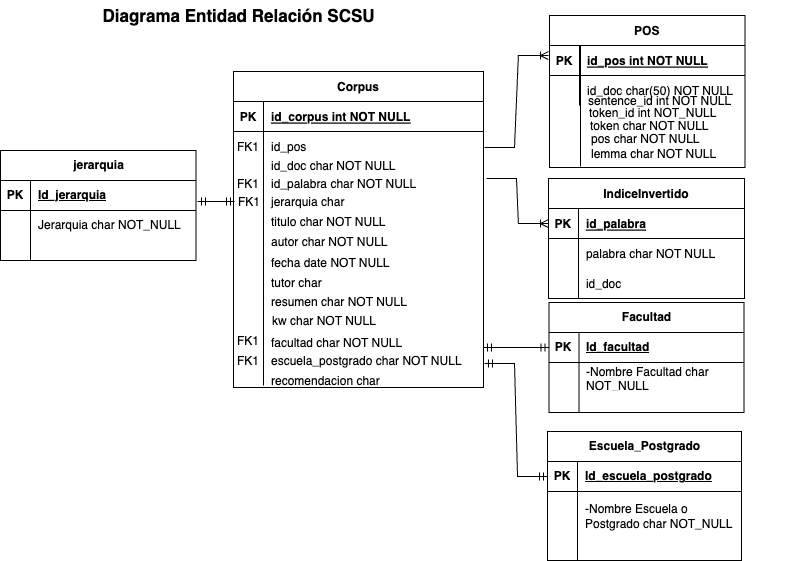
\includegraphics[width=0.8\linewidth]{images/05-desarrollo/4_ciclo/diagrama_entidadrel_SCSU} 

}

\caption{SCSU: Diagrama entidad relación}\label{fig:diagramer}
\end{figure}

Adicionalmente, a la tabla ``corpus'' se le añade una columna que se corresponde con las ``recomendaciones'' generadas para cada documento, donde se almacena una \emph{string} que corresponde a una estructura de datos html.

\textbf{Diagrama General del Sistema - Versión Contenedores}

En la Figura \ref{fig:diagramacontenedores}, se define la estructura que será implementada, teniendo en cuenta los requerimientos funcionales y no funcionales indicados anteriormente. La propuesta funciona como un sistema distribuido, ver \ref{SD}, ``Sistemas Distribuidos'', donde mediante el uso de contenedores, ver \ref{contenedores}, ``Contenedores'', se crean instancias en las que son ejecutadas los servicios necesarios para que el Sistema Complementario Saber UCV pueda cumplir con los objetivos propuestos. La integración y la asignación de recursos a cada contenedor se hace mediante el uso de un orquestador, ver \ref{orquestador}, ``Orquestadores''.

\begin{figure}

{\centering 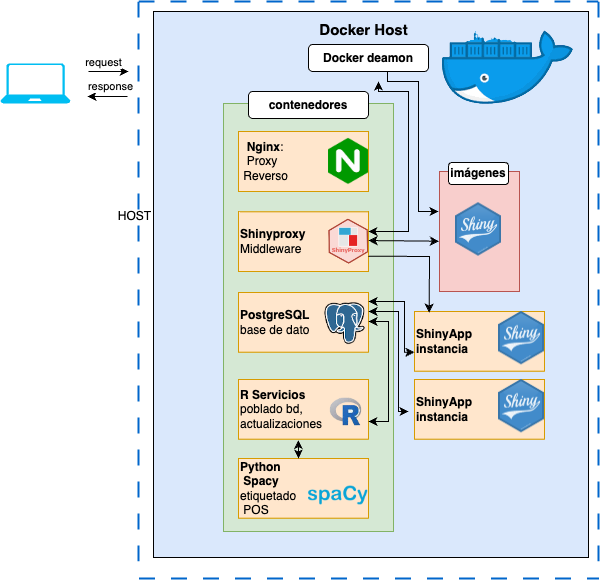
\includegraphics[width=0.8\linewidth]{images/05-desarrollo/4_ciclo/digrama_contenedores_modulos} 

}

\caption{SCSU: Diagrama general del sistema en contenedores}\label{fig:diagramacontenedores}
\end{figure}

En la fase de colaboración de este ciclo se especificarán las tareas y funciones asignadas a cada contenedor.

\textbf{Esquema General de Clasificación y Extracción de Datos del SCSU}

En la Figura \ref{fig:diagramaextra} ,se observa el proceso de extracción y clasificación de datos que realizará el SCSU, obteniendo los valores desde el repositorio Saber UCV, teniendo dos ramas principales que alimentan a la base de datos.

En tal sentido, la lógica de este proceso es que en la primera rama se descarga el documento anexo a cada investigación, cuando se cumplan las condiciones, se hace la lectura del documento y se inicia el proceso de clasificación por facultad y área de estudio, como se vio en \ref{asignacion}, ``Iteración- Extracción y Clasificación de las Investigaciones''.

Por otra parte, en la segunda rama se hace el ``etiquetado del discurso'', que fue revisado en \ref{iternlp}, ``Iteración- Preparación del Corpus''. Es necesario señalar que ambos procesos alimentarán a las correspondientes tablas en la base de datos.

Igualmente se tiene que el proceso indicado, se ejecuta inicialmente para realizar el poblado de la base de datos y también se replica periódicamente, según un parámetro que es definido en el archivo de configuración del orquestador, para proceder a actualizar e incorporar las nuevas investigaciones que se encuentren disponibles en el repositorio Saber UCV.

\begin{figure}

{\centering 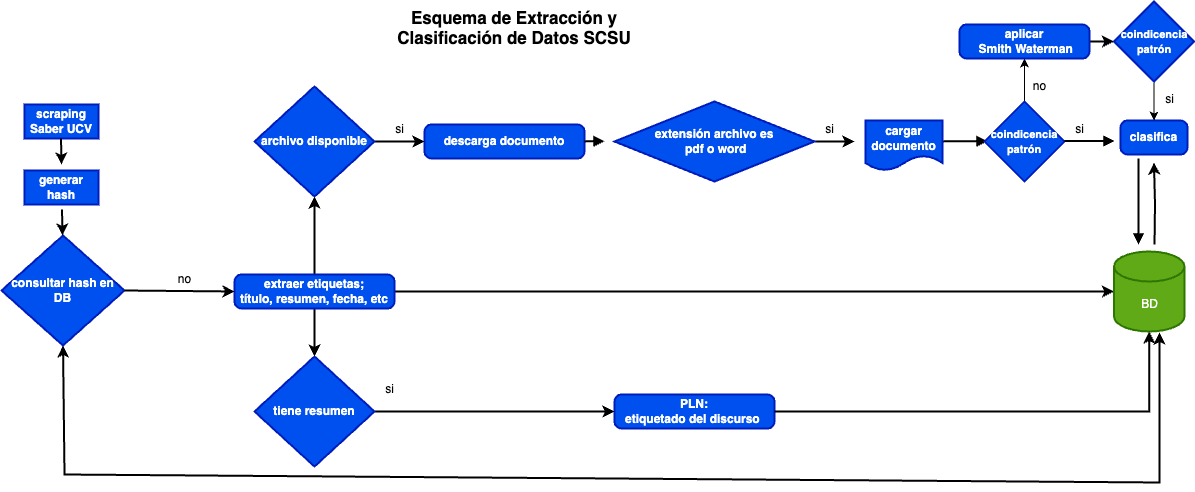
\includegraphics[width=0.9\linewidth]{images/05-desarrollo/4_ciclo/esquema extraccion} 

}

\caption{Esquema extracción y clasificación de datos}\label{fig:diagramaextra}
\end{figure}

\textbf{Interfaz Visual (\emph{Mock Up})}

La interfaz cuenta con tres componentes:

\begin{enumerate}
\def\labelenumi{\arabic{enumi}.}
\item
  \textbf{Sidebar:} en la barra lateral que se ubicará en la parte izquierda de la aplicación y es el área donde el usuario definirá el texto de búsqueda, así como los paremetros que le acompañan. En la Figura \ref{fig:sidebar2}, se puede ver el diseño propuesto.

  \begin{figure}

  {\centering 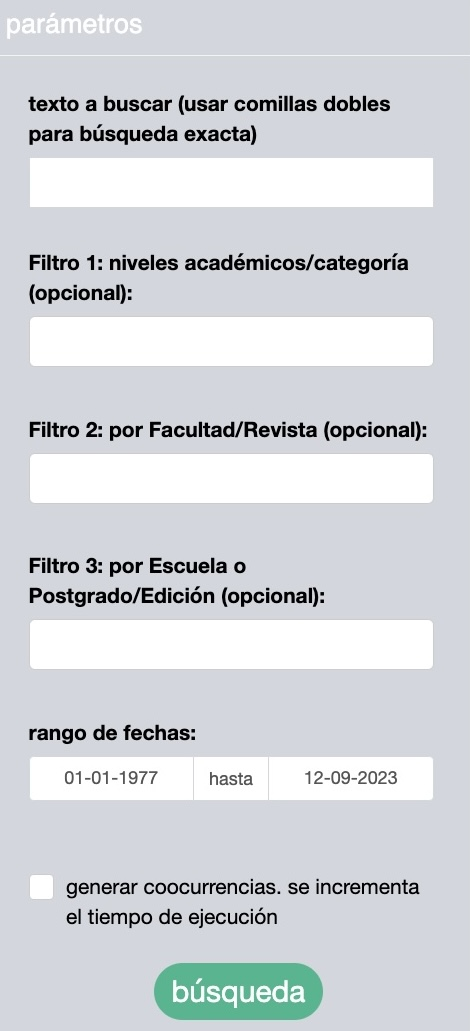
\includegraphics[width=0.35\linewidth]{images/05-desarrollo/4_ciclo/UI/sidebar} 

  }

  \caption{Interfaz de usuario - Sidebar}\label{fig:sidebar2}
  \end{figure}
\item
  \textbf{Main Tabs:} es la sección de pestañas que se encontrará en la parte media alta de la aplicación y es donde el usuario podrá seleccionar la visualización de los ``tabla resultados'', bien sea para la tabla de los documentos o para ver los mapas de conocimiento. En la Figura \ref{fig:maintab}, se representa la propuesta. Al seleccionar una pestaña está cambiará el color de fondo verde a gris.

  \begin{figure}

  {\centering 
\includegraphics[width=0.9\linewidth]{images/05-desarrollo/4_ciclo/UI/maintab} 

  }

  \caption{Interfaz de usuario - Pestañas }\label{fig:maintab}
  \end{figure}
\item
  \textbf{Resultados:} debajo de ``Main Tabs'' se presentan los resultados obtenidos en el proceso de búsqueda. La representación es contextual basada en la selección de pestaña que está seleccionada (``tabla resultados'' o ``mapas de conocimiento'').

  \begin{enumerate}
  \def\labelenumii{\arabic{enumii}.}
  \item
    En la Figura \ref{fig:tablaresultados2}, se puede ver la representación de la tabla de resultados de una búsqueda.

    \begin{figure}

    {\centering 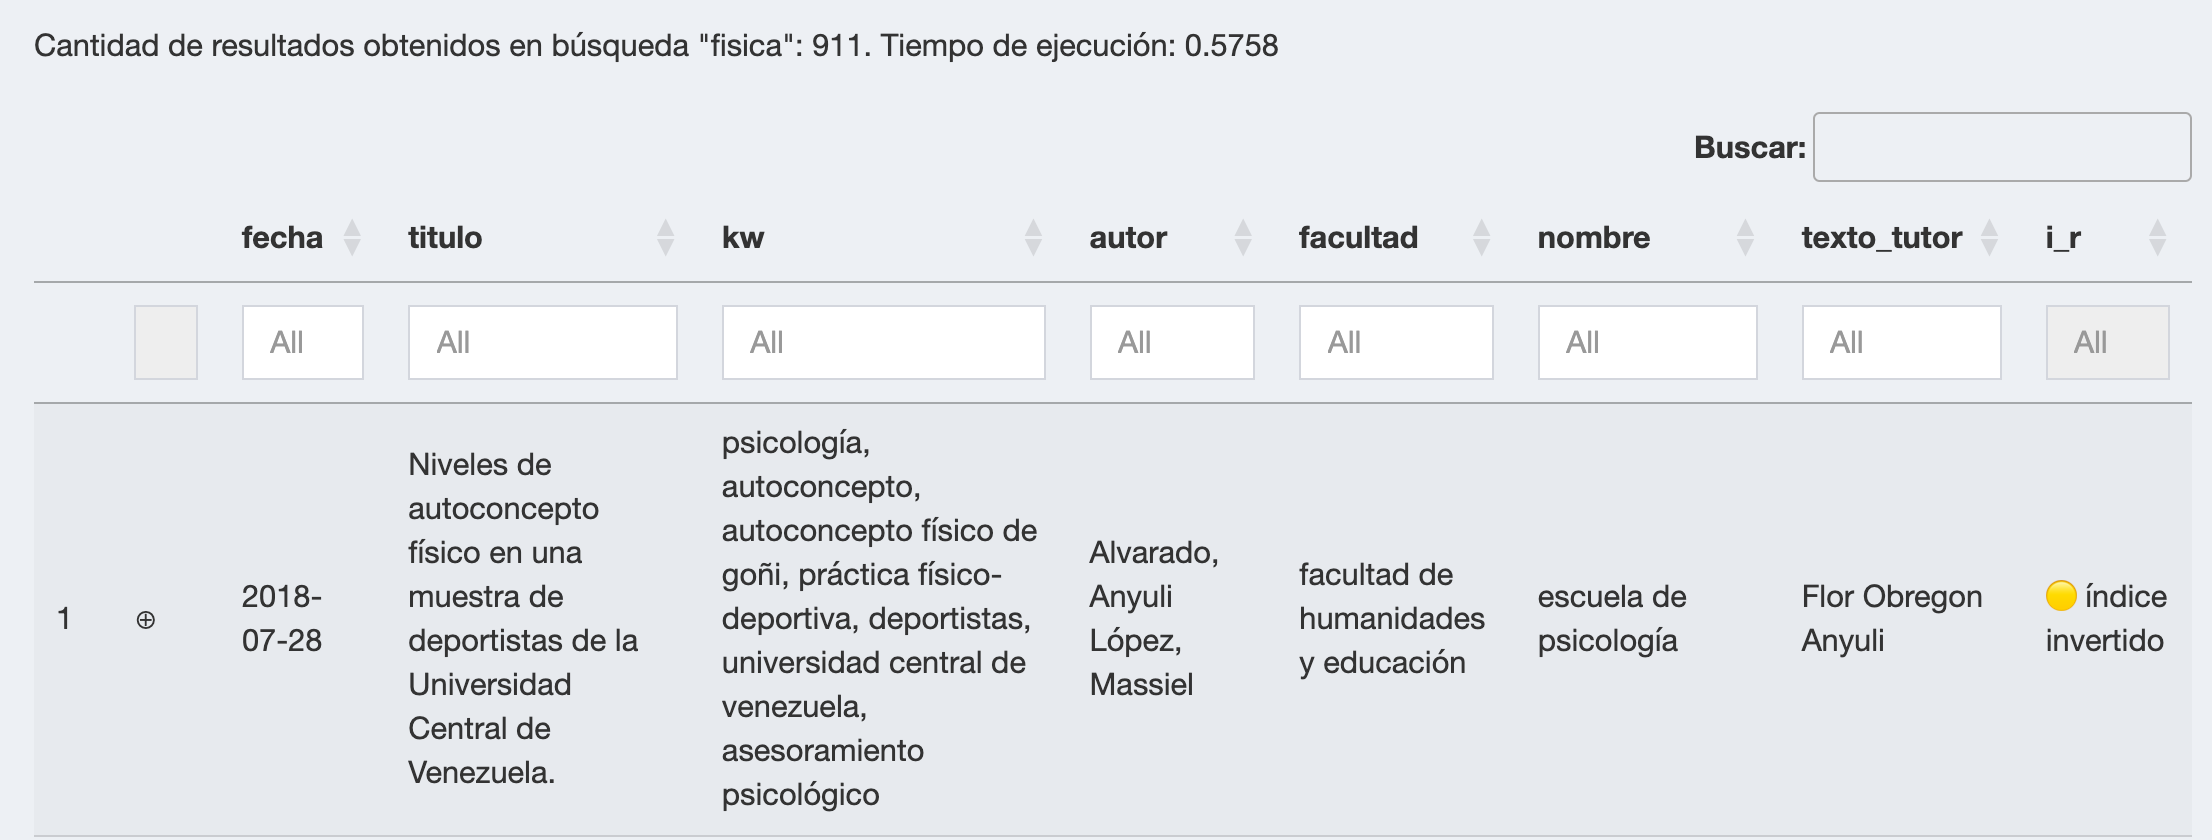
\includegraphics[width=0.9\linewidth]{images/05-desarrollo/4_ciclo/UI/tablaresultado} 

    }

    \caption{Interfaz de usuario - Tabla resultados de búsqueda}\label{fig:tablaresultados2}
    \end{figure}
  \item
    En las Figura \ref{fig:tablaresultados3}, se puede ver la representación propuesta de mapas de conocimiento.

    \begin{figure}

    {\centering 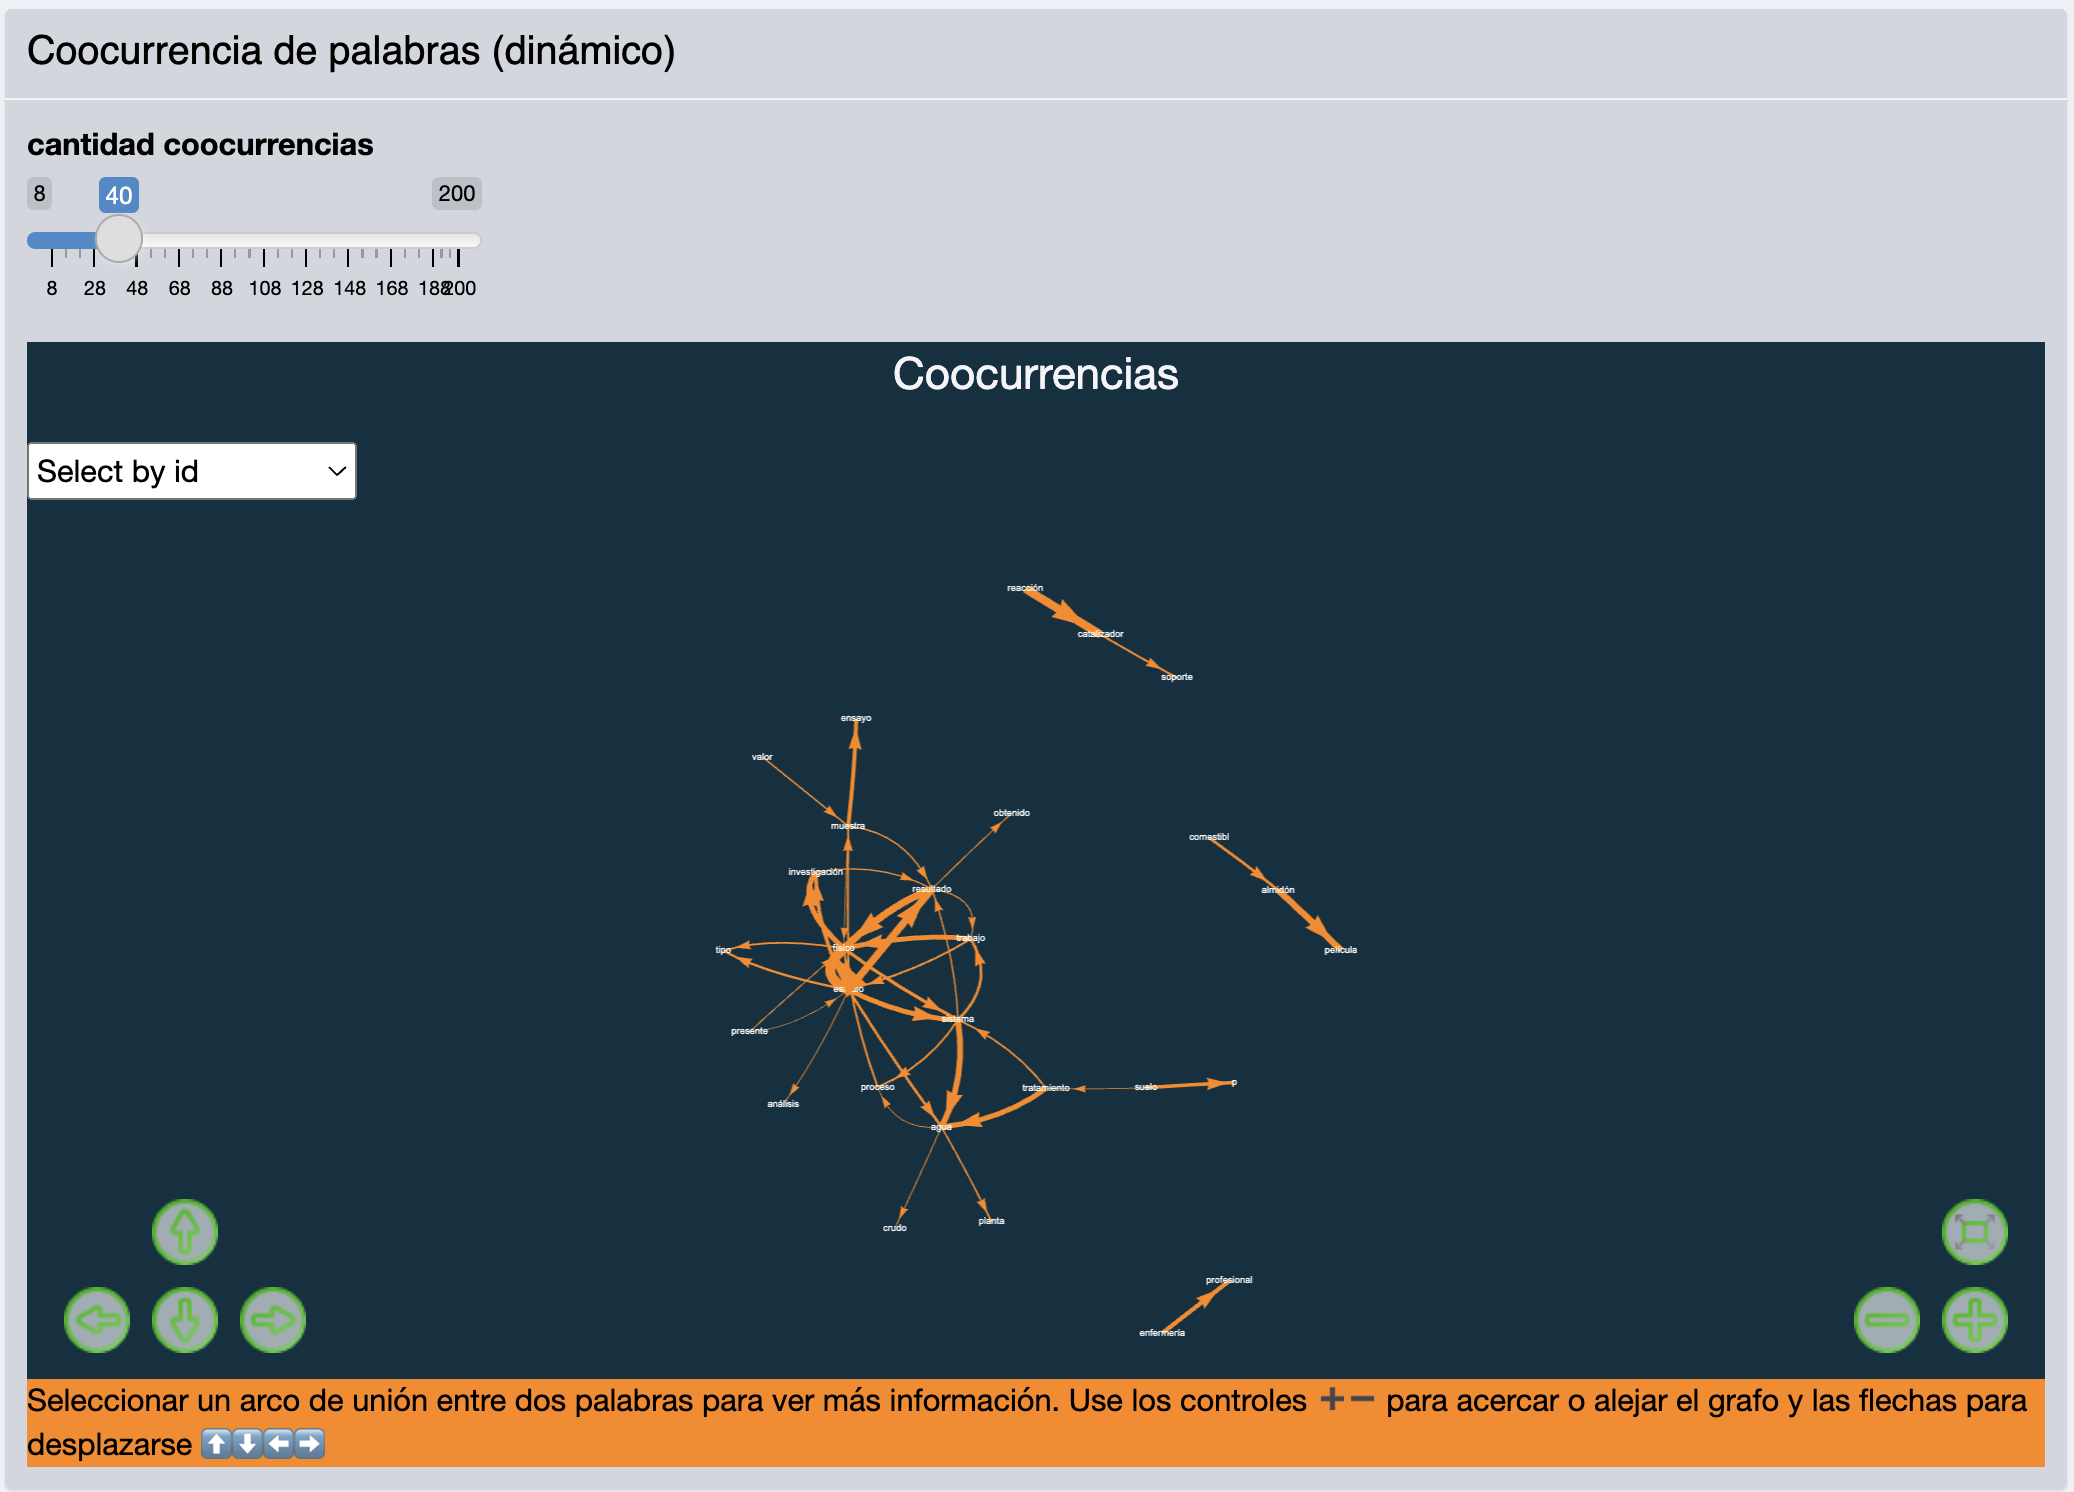
\includegraphics[width=0.7\linewidth]{images/05-desarrollo/4_ciclo/UI/uimapas} 

    }

    \caption{Interfaz de usuario - Mapas de conocimiento}\label{fig:tablaresultados3}
    \end{figure}
  \end{enumerate}
\end{enumerate}

Adicional a estos tres componentes, la propuesta de interfaz incluye:

\begin{enumerate}
\def\labelenumi{\arabic{enumi}.}
\item
  \textbf{Tooltips}: al hacer \emph{hoover} por áreas de introducción o selección de valores se desplegará un texto de ayuda según se ve en la Figura \ref{fig:tooltip}.

  \begin{figure}

  {\centering 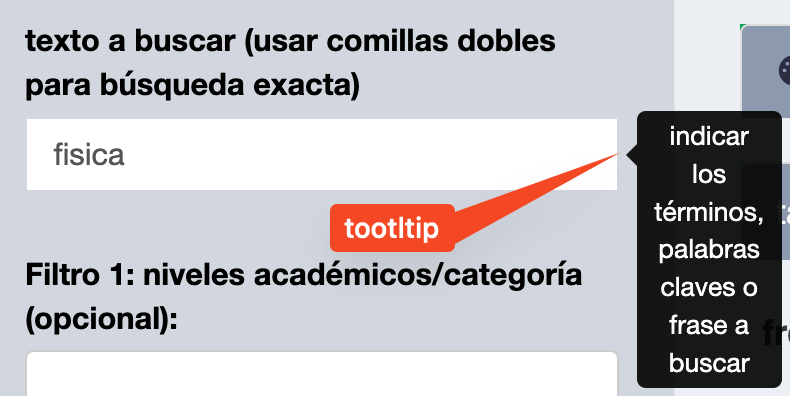
\includegraphics[width=0.3\linewidth]{images/05-desarrollo/4_ciclo/UI/tooltip} 

  }

  \caption{Interfaz de usuario - Tooltips }\label{fig:tooltip}
  \end{figure}
\item
  \textbf{Inspección documento:} la tabla de resultados dispondrá de un ícono ``+'' que expande la tabla para mostrar el detalle y recomendaciones de un documento, como se observa en la Figura \ref{fig:detalledoc}.

  \begin{figure}

  {\centering 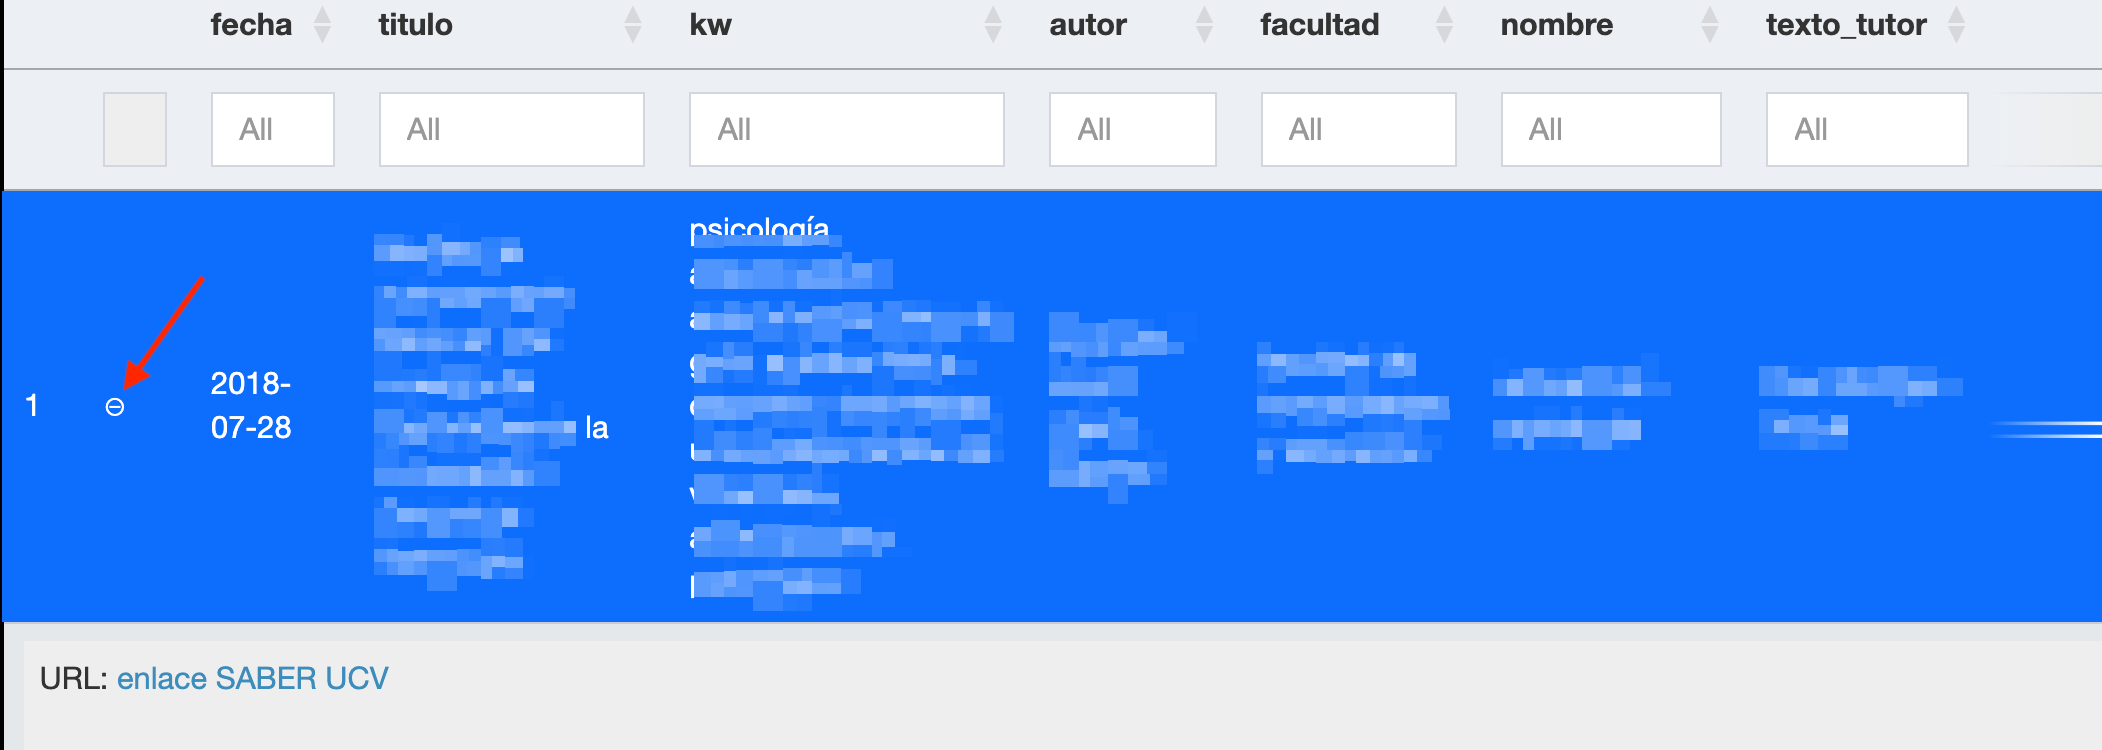
\includegraphics[width=0.8\linewidth]{images/05-desarrollo/4_ciclo/UI/uiinspecciontabla} 

  }

  \caption{Interfaz de usuario -Inspección documento }\label{fig:detalledoc}
  \end{figure}
\item
  \textbf{Inspección mapas de conocimiento:} la propuesta de visualización del detalle de aparición en documentos de una determinada coocurrencia de dos palabras que se encuentran unidas por un arco se ven en la Figura \ref{fig:detallemc}. La tabla que se muestra aparecerá mediante una ventana desplegable.

  \begin{figure}

  {\centering 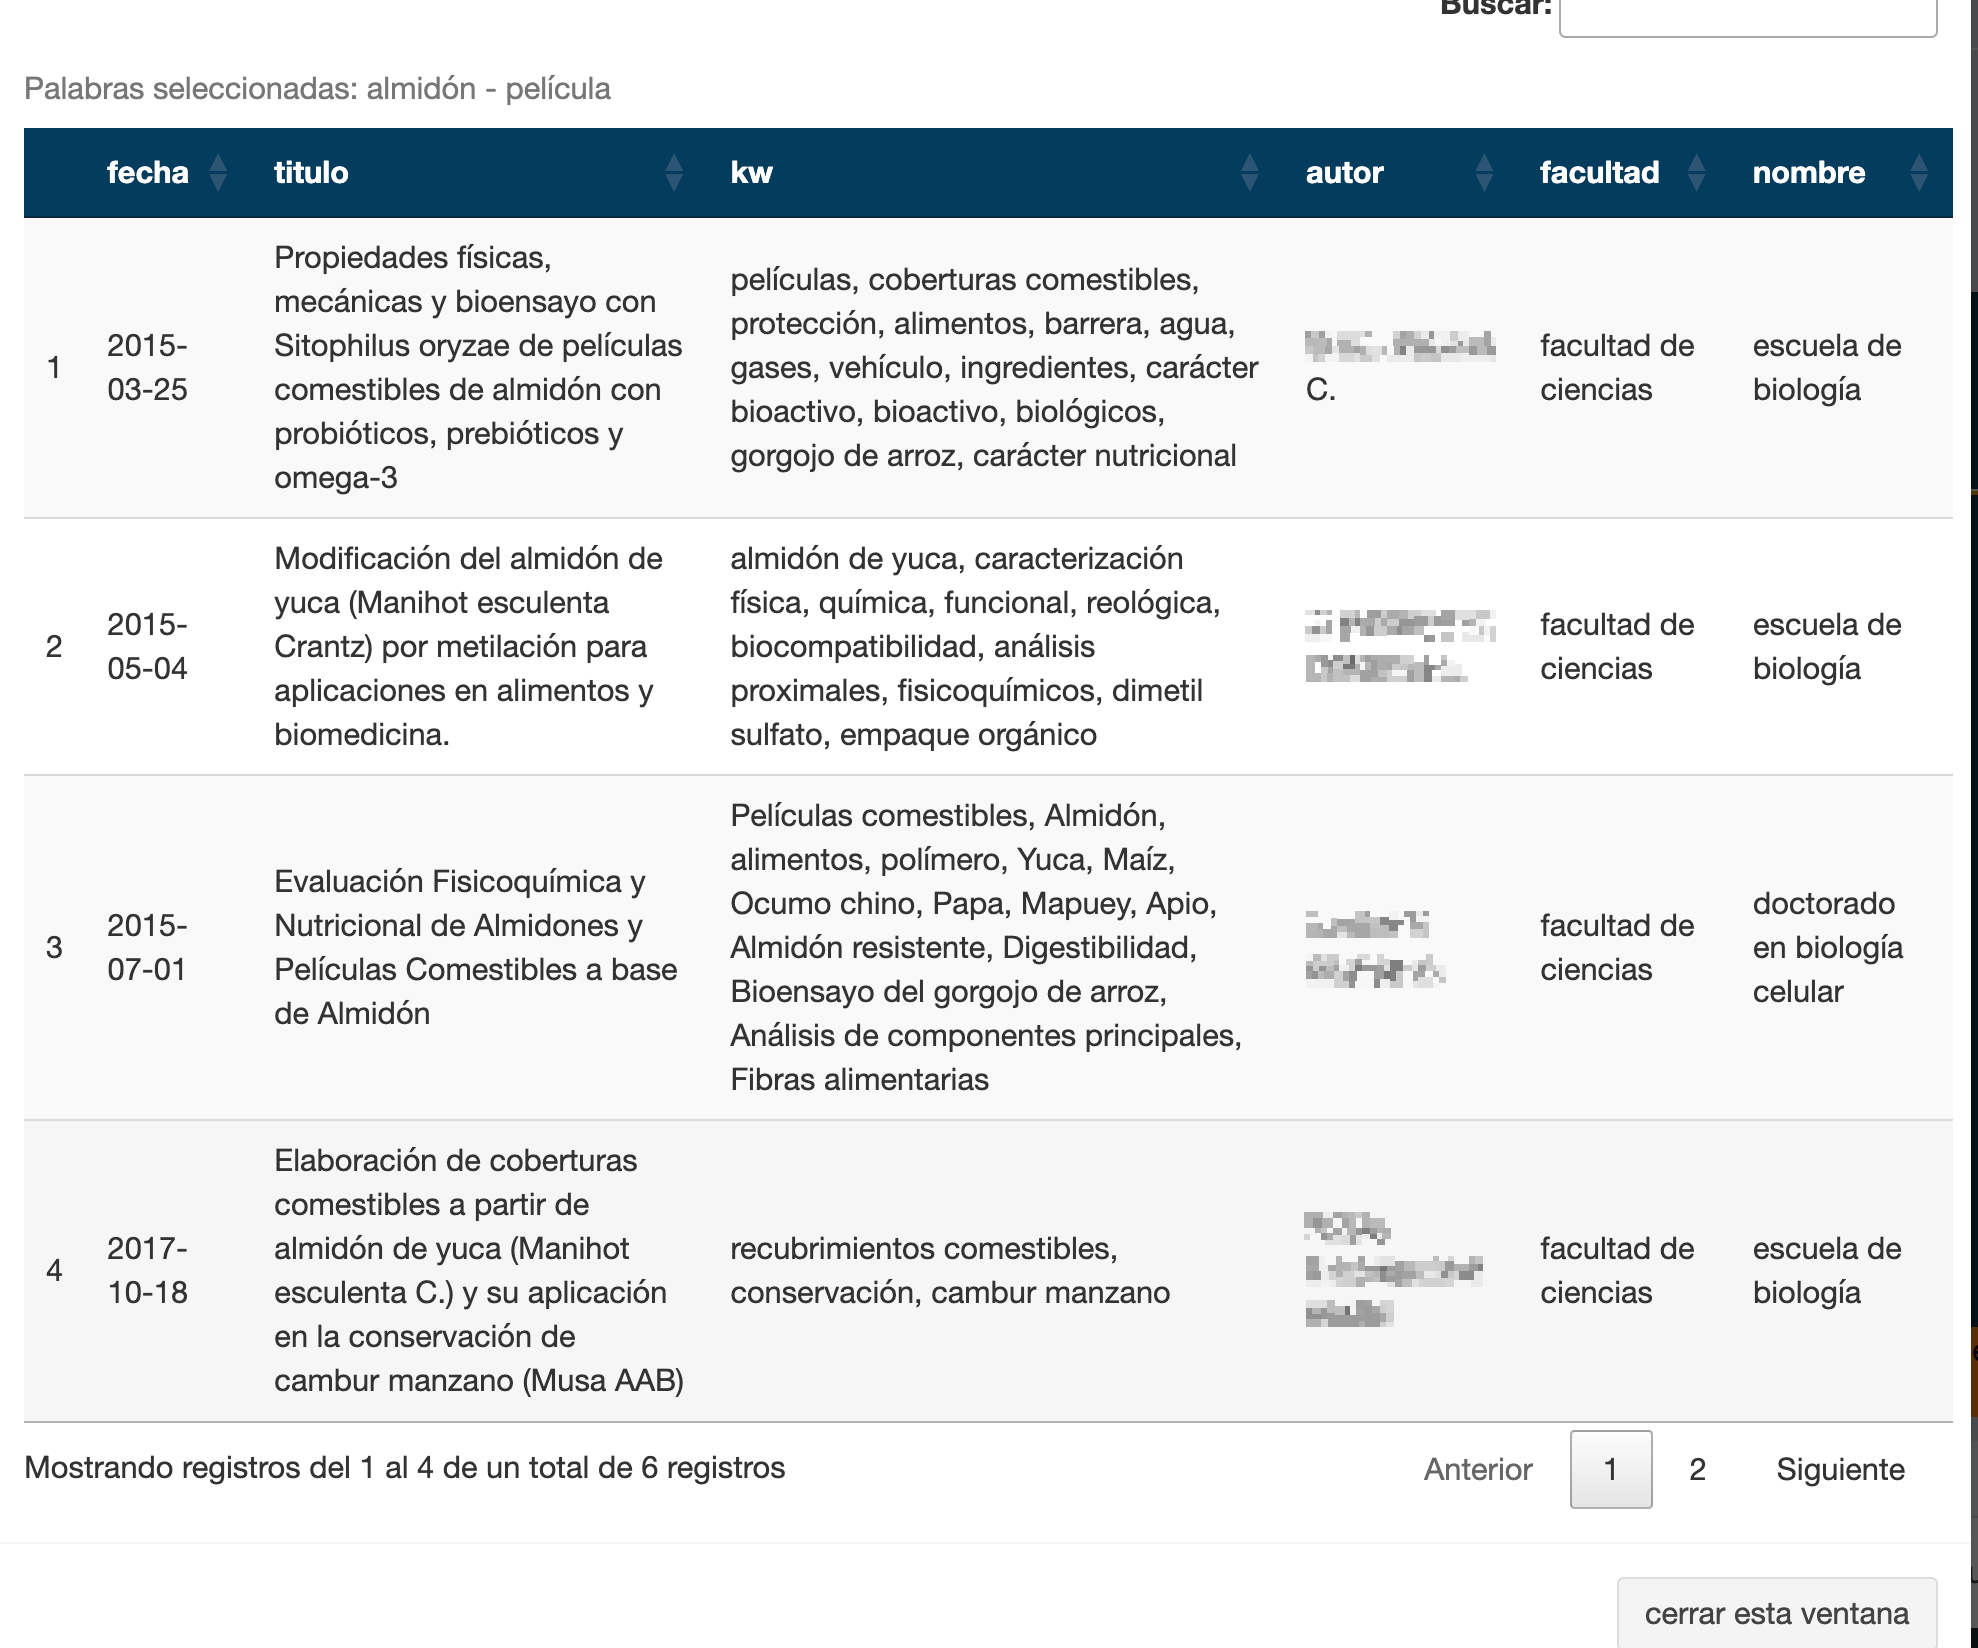
\includegraphics[width=0.6\linewidth]{images/05-desarrollo/4_ciclo/UI/uiinspeccionmapas} 

  }

  \caption{Interfaz de usuario- Inspección mapas de conocimiento }\label{fig:detallemc}
  \end{figure}

  \newpage
\end{enumerate}

\textbf{Módulos Aplicación Web}

La aplicación web, que será desarrollada en el \emph{framework} Shiny, según las prácticas de desarrollo recomendadas, se hace bajo la arquitectura de módulos denominados ``Shiny modules'', descomponiendo en partes independientes cada par de funciones relacionadas en la ui (define la interfaz de usuario) y el \emph{server} (define la lógica del servidor), facilitando la comprensión del funcionamiento de la aplicación, la legibilidad del código, pruebas unitarias y el mantenimiento (\protect\hyperlink{ref-wickham2021}{Wickham 2021}). En la Figura \ref{fig:shinymodulo}, se puede ver la arquitectura de la aplicación que se integrará dentro del sistema distribuido.

\begin{figure}

{\centering \includegraphics[width=0.6\linewidth]{images/05-desarrollo/4_ciclo/digrama_shinyapp_modulos} 

}

\caption{Diagrama aplicación web Shiny versión modular}\label{fig:shinymodulo}
\end{figure}

\textbf{Colaboración}

Según lo propuesto en la fase de Especulación, se hizo el desarrollo del sistema mediante un conjunto de contenedores orquestados, tomando en consideración que es necesario implementar los mecanismos de comunicación necesarios con la definición de una red y de disponer de un volumen compartido con la máquina \emph{host}.

Hay que destacar que, en la implementación se usaron ampliamente los conocimientos adquiridos en ciclos anteriores, no obstante también se tuvieron que revisar documentaciones, probar distintas opciones de librerías e imágenes de contenedores que permitiesen llevar a un entorno de producción el sistema planificado con la debida integración de los componentes.

\textbf{Contenedores}

Para realizar la implementación del sistema, apoyado en contenedores para los distintos servicios que lo conforman, se eligió Docker como herramienta. Mediante un archivo denominado ``Dockerfile'' para cada servicio se especificó el entorno, dependencias y configuraciones necesarias para crear la imagen que servirá para instanciar cada contenedor.

A continuación se indican los contenedores que forman parte del sistema y los puertos que disponden para interactuar unos con otros:

\begin{enumerate}
\def\labelenumi{\arabic{enumi}.}
\item
  \textbf{Nginx:} es el servidor web/proxy inverso de código abierto que en este sistema se usa para redireccionar las peticiones del cliente recibidas en el puerto 80 y 443 al puerto 8080. En este contenedor también se almacena el certificado SSL para permitir conexiones por el protocolo HTTPS en caso de configurar un dominio \footnote{Al momento de presentar este Trabajo de Grado no se dispone de un dominio para realizar la configuración del certificado para conexiones HTTPS, no obstante en un momento previo en que se tenía disponible un dominio se hicieron las pruebas para comprobar la integración y correcto funcionamiento.}. Este contenedor fue creado desde la imagen oficial de NGINX que se encuentra en el Docker Hub \footnote{Docker Hub: es un repositorio donde se pueden compartir, almacenar y encontrar imágenes de contenedores.} sin añadir ninguna capa (\emph{layer}) adicional.
\item
  \textbf{Cerbot:} es una herramienta de código abierto que permite tramitar y habilitar las conexiones mediante el protocolo HTTPS con el uso de un certificado ``Let´s Encrypt''. El uso de este certificado está asociado al uso de un dominio en el \emph{deploy} de la aplicación. Este contenedor fue instanciado desde una imagen de CERBOT del Docker Hub sin realizar ninguna modificación.
\item
  \textbf{Shinyproxy:} es una solución de código abierto para alojar aplicaciones Shiny (\protect\hyperlink{ref-shinyproxy2023}{{«Shinyproxy»} 2023}) que cuenta con una tecnología estable y probada. El uso de este contenedor se justifica en el hecho de que una aplicación Shiny funciona como ``\emph{single thread}'' y es necesario que ante cada petición de acceso, al servidor despliegue un \emph{workspace} completamente aislado, es decir, un contenedor distinto. Shinyproxy es una implementación del servidor \emph{Spring Boo}t que tiene la capacidad de hacer la replicación indicada y permite controlar los recursos de memoria y \emph{CPU} asignados, así como el \emph{timeout} a cada instancia que se despliega. Otras ventajas que aporta, no implementadas en esta versión del sistema, es que permite establecer \emph{login} en el uso de la aplicación y la creación de grupos de usuarios con perfiles distintos, contando con soporte para distintos métodos de autenticación. Si bien en estos momentos la aplicación está concebida para el libre acceso, en algún momento se pude restringir y no sería necesario hacer modificaciones en la arquitectura, más allá de variaciones en el archivo de configuración. Este contenedor habilita el puerto 8080 para escuchar las peticiones y fue generado desde la imagen almacenada en el Docker Hub, Shinyproxy.
\item
  \textbf{Shiny Web App}: en la imagen creada se encuentra la aplicación web con todas las dependencias y librerías necesarias para remitir los \emph{queries} al contenedor del manejador de la base de datos, presentar los resultados y generar las visualizaciones correspondientes. Como se indicó anteriormente, cada vez que ocurre desde el navegador del cliente una petición de acceso, desde el contenedor Shinyproxy , se crea una instancia de esta imagen con todos los elementos necesarios para que la \emph{app} funcione. En caso de presentar alguna falla, el sistema es tolerante a los mismos, porque se pueden seguir recibiendo peticiones que replicarían un contenedor nuevo desde la imagen sin afectar al contenedor que presentase el fallo, o viceversa. Desde cada contenedor instanciado de esta imagen se realiza el acceso de lectura al contenedor que contiene PostgreSQL\emph{,} donde reposa la base de datos que contiene los textos ya procesados. La imagen que se usa en este servidor fue definida a medida de las necesidades.

  \textbf{Lógica de la Aplicación}

  El esquema general de la aplicación es similar al que se presentó en el prototipo en la Figura \ref{fig:esqshinyproto}. A continuación se mencionan las entradas y salidas que se generan dentro del contenedor.

  \begin{enumerate}
  \def\labelenumii{\arabic{enumii}.}
  \item
    \textbf{Entradas:} el usuario indica y selecciona los siguientes valores.

    \begin{enumerate}
    \def\labelenumiii{\roman{enumiii}.}
    \item
      \textbf{Definición \emph{query}:} contiene un campo para la entrada de texto con el que se generará el \emph{query}. Muestra tablas precargadas para seleccionar:

      \begin{enumerate}
      \def\labelenumiv{\arabic{enumiv})}
      \item
        Nivel académico del trabajo - opciones: pregrado, especialización, maestría y doctorado.
      \item
        Facultad o centro de adscripción - opciones: 11 facultades más un centro (CENDES).
      \item
        Nombre del pregrado o postgrado - opciones: 412 (50 carreras de pregrado y 362 postgrados).
      \end{enumerate}

      Cada una de las tablas anteriores se actualiza dinamicamente según se vayan seleccionando las relaciones y las disponibilidades. P. ej., al seleccionar pregrado solo se mostrarán los nombres de las carreras de pregrado, pero si se selecciona también el nombre de la facultad, solo se mostrarán las carreras de pregrado dentro de la facultad seleccionada. Para un determinado filtro se permiten selecciones múltiples dando una total flexibilidad al momento de ejecutar los \emph{queries}. El texto del \emph{query} es procesado convirtiéndolo a minúsculas y removiendo signos de puntuación. En caso de indicar el texto entre comillas el sistema aplicará el método de búsqueda exacta.
    \item
      \textbf{Selector ``Generar Coocurrencias'':} es una casilla que sirve para seleccionar si se van a representar los mapas de conocimiento o no. Por defecto está deseleccionado ya que la representación de los mapas incrementa el tiempo de procesamiento.
    \item
      \textbf{Clic ``Inspeccionar Documento'':} al obtener los resultados en una tabla se puede inspeccionar un documento particular para ver el texto resumen y las recomendaciones de documentos similares.
    \item
      \textbf{Cantidad de Coocurrencias:} teniendo como condición que previamente se seleccionara ``generar coocurrencias'', dentro de la pestaña de ``coocurrencias'', correspondientes a los mapas de conocimiento, se puede modificar la cantidad de coocurrencias a representar. El valor por defecto representado es 60.
    \item
      \textbf{Clic ``Inspeccionar Mapas de Conocimiento'':} dentro de la pestaña de ``coocurrencias'', correspondientes a los mapas de conocimiento, al tener representadas dos palabras mediante nodos existe un arco que las une. Sobre el arco se puede hacer clic e inspeccionar los documentos que contienen las palabras asociadas por el arco.
    \end{enumerate}
  \item
    \textbf{Salidas:} Ante el \emph{query} se genera.

    \begin{enumerate}
    \def\labelenumiii{\roman{enumiii}.}
    \item
      \textbf{Resultados Query:} en una tabla creada con la librería DT se muestra el listado de documentos recuperados mostrando en cada fila los siguientes atributos: autor, fecha, palabras clave, texto resumen, nombre tutor. Los documentos a presentar y el orden en que son presentados viene desde el contenedor PostgreSQL. Adicionalmente se muestra un enlace al repositorio Saber UCV donde se encuentra alojado el respectivo trabajo (el documento en PDF). Igualmente se presentan los textos que tienen mayor similitud con el documento seleccionado. Un gráfico con la frecuencia por año de los trabajos extraídos mediante el \emph{query}. El gráfico se genera con la librería apexcharter, por lo cual tiene ciertas interactividades mostrando con el \emph{hoover} el valor de la cantidad por año que está representada en cada columna.
    \item
      \textbf{Mapas de Conocimiento Dinámico:} gráfico de coocurrencia interactivo de palabras que se genera mediante la librería de VisNetwork. Este gráfico permite distintas interacciones con el usuario como hacer \emph{zoom (in-out)}, seleccionar un determinado nodo, usar las teclas izquierda, derecha, arriba y abajo del teclado, así como también permite seleccionar un arco de unión entre dos palabras coocurrentes. Al realizar la selección se filtra un subconjunto de los documentos que contienen ambas palabras representadas por nodos. Los documentos filtrados se mostrarán en una tabla contigua, también generada en DT, donde solo se incluye el texto resumen de cada trabajo.
    \item
      \textbf{Mapas de Conocimiento Estático:} gráfico de coocurrencias estático de palabras, donde mediante la librería ggraph son generados un par de gráficos con distintas granularidades. El primero exhibe la misma coocurrencia de palabras expuesta en el punto con una visualización estática. En cuanto a la granularidad, se muestran las palabras que coocurren dentro de todo el resumen independientemente de la proximidad que tengan. El segundo gráfico también muestra la coocurrencia, pero solo de palabras que se encuentran en el texto resumen una seguida de otra representando los resultados con una menor granularidad. Con la librería UDPipe se generan las estructuras de datos necesarias para generar los grafos (arcos y nodos).
    \end{enumerate}

    En el Apéndice se listan los paquetes que usa este contenedor.
  \end{enumerate}
\item
  \textbf{PostgreSQL:} es el contenedor donde se encuentra el manejador de PostgreSQL versión 16 y en él se almacenan todas las tablas que usa el sistema. También recae la funcionalidad de generar el ``\texttt{ts\_vector}'', convertir el query a un ``\texttt{ts\_query}'' y mediante la función ``\texttt{ts\_rank}'' reordenar los resultados extraídos con base en un ranking junto con el indexado de las distintas tablas. En el ciclo \ref{desarrollociclos3}, ``Iteración- Implementación Prototipo'', se indican más detalles sobre las funciones señaladas. En este contenedor se instanció desde una imagen de PostgreSQL versión 16.1 extraída del Docker Hub, a la cual no le fue realizada ninguna modificación distinta a la configuración para la definición de usuarios, contraseña y la ruta de un volumen compartido con el \emph{host} para garantizar que se tengan ``datos persistentes''. Este contenedor recibe consultas del contenedor \textbf{``}Shiny Web App'' y escritura-lectura desde el contenedor ``R Imagen Servicios'' teniendo habilitado el puerto 5432.
\item
  \textbf{R Imagen Servicios}: en este contenedor se creó una imagen con todos los servicios necesarios para realizar el \emph{web crawling}, el procesamientos de textos y la descarga de los archivos desde Saber UCV para realizar la clasificación de las tesis y demás trabajos. Al iniciar la configuración del sistema, contiene las funcionalidades que permiten realizar la creación de la base de datos, las tablas y el poblado de estas. Periódicamente es invocado un \emph{script} mediante un ``cron job'' para realizar los procesos de incorporación de aquellos documentos nuevos que se detecte que están disponibles en Saber UCV. La imagen base que se usa es la del proyecto Rocker (\protect\hyperlink{ref-RJ-2017-065:2017}{Boettiger y Eddelbuettel 2017}), la cual es una versión ampliamente probada y optimizada por la comunidad de usuarios de R.

  \textbf{Procesos:} los procesos que se ejecutan en este contenedor se listan a continuación.

  \begin{enumerate}
  \def\labelenumii{\roman{enumii}.}
  \tightlist
  \item
    \textbf{Poblado Base de Datos:} se ejecutan los procesos para hacer el poblado inicial de base de dato así como a la creación del indexado de la base de datos en el contenedor PostgreSQL\textbf{.} En la fase de especulación de este ciclo se presentó un diagrama que describe en el esquema de la Figura \ref{fig:diagramaextra}, ``extracción y clasificación de los datos''.
  \item
    \textbf{Descarga de Datos:} proceso que fue abordado en el ciclo \ref{desarrollociclos1}, ``Ciclo Conformación del Conjunto de Datos''.
  \item
    \textbf{Text Mining y NLP:} en el ciclo \ref{desarrollociclos3}, ``Ciclo Prototipo SCSU'', en la iteración \ref{iternlp}, ``Preparación del Corpus'', se detallan los procesamientos a los textos que ahora son ejecutados en este contenedor. La diferencia es que para usar spacyr, al depender esta librería de una ambiente virtual en Python , es necesario configurar otro contenedor con las dependencias y librerías que permitan el llamado al etiquetado del discurso. El contenedor que se integra para realizar estos procesos es \textbf{``}Python Spacy''\textbf{.}
  \item
    \textbf{Generación de Recomendaciones:} se corresponde con detallado en el ciclo \ref{desarrollociclos3}, ``Ciclo Prototipo de SCSU'', en la iteración \ref{imrecomendacion}, ``Recomendación de Documentos''.
  \end{enumerate}

  En el Apéndice de esta investigación se listan las librerías que usa este contenedor.
\item
  \textbf{Python Spacy:} se creó una imagen que está basada en ``Ubuntu 22'' con ``Python 3.10'', la librería ``spaCy v.3'' y el modelo de spaCy ``es\_core\_news\_lg''. Su función es que mediante un volumen compartido pueda ser invocado desde el contenedor ``R Imagen Servicios'' para así realizar los procesamientos de NLP descritos.

  \newpage
\end{enumerate}

\textbf{Orquestador}

Todos los contenedores mencionados es necesario que actúen de forma coordinada, compartiendo recursos como una red y volúmenes de almacenamiento. Para lograr esto se acude a la herramienta ``Docker Compose'' que se instala en el \emph{host} y permite simplificar y automatizar el despliegue de aplicaciones compuestas por múltiples servicios y contenedores en entornos de desarrollo y producción.

Es necesario señalar que un archivo YAML, denominado ``Docker-compose.yml'', se define la infraestructura, configuración y gestión de una aplicación, donde se encuentran detallados los servicios, contenedores, redes y volúmenes necesarios para la aplicación, así como las relaciones y configuraciones entre ellos, simplificando la orquestación de los contenedores.

También la adopción de Docker Compose facilita la replicación del entorno de desarrollo en diferentes máquinas, mejorando la consistencia en el desarrollo. Es necesario indicar que, la responsabilidad del administrador queda reflejada en la definición de distintas variables de entorno contenidas en el archivo Docker compose, como lo es la definición del período de actualización de los textos.

\textbf{Mantenimiento del SCSU}

De acuerdo a la implementación del sistema, los procesos de mantenimiento que corresponde ejecutar al administrador son los que se detallan a continuación:

\begin{enumerate}
\def\labelenumi{\arabic{enumi}.}
\item
  Respaldos Regulares de la Base de Datos:

  \begin{itemize}
  \tightlist
  \item
    Se estableció un ``\emph{cron job}'' en el contenedor ``R Imagen Servicios'' para realizar respaldos automáticos de la base de datos que maneja el contenedor ``PostgreSQL''.
  \end{itemize}
\item
  Monitoreo del rendimiento:

  \begin{itemize}
  \tightlist
  \item
    Se utilizan herramientas de monitoreo para vigilar el rendimiento del contenedor ``PostgreSQL'', ``Shinyproxy'' y ``Shiny''.
  \end{itemize}
\item
  Logs y registro de eventos:

  \begin{itemize}
  \item
    Registro de \emph{logs} de contenedores en un volumen compartido con el \emph{host}.

    \newpage
  \end{itemize}
\item
  Gestión de dependencias:

  \begin{itemize}
  \tightlist
  \item
    Se documentan las dependencias específicas de la versión de PostgreSQL, Shinyproxy y Shiny.
  \end{itemize}
\item
  Seguridad de red:

  \begin{itemize}
  \tightlist
  \item
    Se configuró el \emph{firewall} y las reglas de red para limitar el acceso no autorizado a los contenedores.
  \end{itemize}
\item
  Escalabilidad:

  \begin{itemize}
  \tightlist
  \item
    Se realizaron pruebas de carga para identificar posibles cuellos de botella.
  \end{itemize}
\end{enumerate}

Eventualmente, en caso del sistema quedar en un entorno de producción permanente, sería necesario agregar los siguientes procesos al mantenimiento:

\begin{enumerate}
\def\labelenumi{\arabic{enumi}.}
\item
  Actualizaciones de seguridad:

  \begin{itemize}
  \tightlist
  \item
    Supervisar actualizaciones de seguridad para PostgreSQL y la imagen de Shiny.
  \end{itemize}
\item
  Control de versiones:

  \begin{itemize}
  \tightlist
  \item
    Utilizar un sistema de control de versiones para el código del SCSU.
  \end{itemize}
\item
  Documentación:

  \begin{itemize}
  \tightlist
  \item
    Mantener actualizada la documentación del sistema, incluyendo la configuración, dependencias y procedimientos de recuperación ante desastres.
  \end{itemize}
\end{enumerate}

\textbf{Requerimientos Mínimos de \emph{Hardware}}

Para una concurrencia de 4 usuarios simultáneos, estos son los requerimientos de \emph{hardware}:

\begin{itemize}
\tightlist
\item
  2 CPU virtual
\item
  4 GB de memoria RAM
\item
  50 GB de disco duro
\end{itemize}

\textbf{Aprender}

Este ciclo trajo un profundo y largo proceso de aprendizaje ya que el desarrollo implicó integrar distintos elementos abordados previamente de forma aislada, más el reto de encontrar componentes que fuesen compatibles y adaptados a los requerimientos funcionales y no funcionales planteados.

Igualmente se tiene que, la utilidad de esta integración también representa en que se cuenta con un \emph{framework} que permite desplegar otro tipo de aplicaciones que pueden ser fácilmente escalables en entornos de producción o añadir módulos distintos al SCSU como pudiera ser una aplicación para la administración del sistema o consultar estadísticas de uso.

Hay que destacar que, como la cantidad de ciclos e iteraciones ejecutados previamente había sido extenso, en esta ciclo, más allá del reto de la integración y evaluación de componentes no fue de distinta índole el aprendizaje adquirido, sin embargo se decidió incorporar en la interfaz del usuario un gráfico que muestre la frecuencia de aparición de \emph{query} en el tiempo así como una representación estática de los mapas de conocimiento, ya que en esta versión se presenta con una mejor perspectiva la coocurrencia de términos, a diferencia de la versión interactiva que está diseñada para inspeccionar en detalle una determinada aparición de términos.

\hypertarget{objetivos-alcanzados-2}{%
\subsubsection{Objetivos Alcanzados:}\label{objetivos-alcanzados-2}}

\begin{itemize}
\item
  Se implementó el sistema que cumple con el ``Objetivo General'' propuesto en \ref{objegeneral}.
\item
  Se dispone de una versión del sistema que es reproducible.
\item
  Se integraron con éxito los distintos componentes del sistema.
\end{itemize}

\newpage

\hypertarget{desarrollociclos6}{%
\subsection{Ciclo Incorporación de Otras Investigaciones}\label{desarrollociclos6}}

En este ciclo se aborda la incorporación al ``Sistema Complementario Saber UCV'' publicaciones distintas a las investigaciones de pregrado y postgrado de la Universidad Central de Venezuela.

Lo propuesto en este ciclo únicamente tiene como finalidad evaluar si el SCSU se puede usar para alojar revistas de investigación producidas dentro de la Universidad Central de Venezuela o fuera de ella.

\textbf{Especulación}

Para los centros de estudio que generen investigaciones que sean alojadas en un repositorio de datos y se cumpla la estructura donde se disponga de un título para la publicación, una fecha, un autor, palabras claves (opcional) y un texto, es posible replicar los métodos descritos anteriormente para obtener los datos e incorporarlos al SCSU.

Las publicaciones que se incorporarán son:

\begin{enumerate}
\def\labelenumi{\arabic{enumi}.}
\item
  Archivo histórico de la revista ``Gestión I+D'' editada dentro de la Universidad Central de Venezuela por el Postgrado en Gestión de Investigación y Desarrollo de la Facultad de Ciencias Económicas y Sociales.
\item
  Archivo histórico de la revista ``Episteme NS'' editada dentro de la Universidad Central de Venezuela por el Instituto de Filosofía de la Facultad de Humanidades y Educación.
\item
  Archivo histórico de la revista ``Observador del Conocimiento'' editada por el Observatorio Nacional de Ciencia, Tecnología e Innovación, adscrito al Ministerio del Poder Popular para Ciencia y Tecnología.
\item
  Artículo ``El Dorado Revisitado'' del Boletín Antropológico editado por la Universidad de los Andes.
\end{enumerate}

\textbf{Colaboración}

Siguiendo las técnicas descritas en \ref{scrapeo}, ``Iteración-Extracción de Datos web Saber UCV'', se hizo la descarga de los datos y se introdujeron a la base de datos sin alterar la estructura que se había propuesto en el ciclo \ref{desarrollociclos4}, ``Ciclo de Integración de los Componentes'', lo que motiva a que no se entre en detalles sobre los métodos aplicados para incorporar este nuevo lote de investigaciones.

Luego de hacer la descarga y procesamiento de los datos se obtuvieron la siguiente cantidad de artículos por revista:

\begin{enumerate}
\def\labelenumi{\arabic{enumi}.}
\item
  Gestión I+D (UCV): 129
\item
  Revista Episteme (UCV): 68
\item
  Revista Observador del Conocimiento (ONCTI): 197
\item
  Boletín Antropológico (ULA): 1
\end{enumerate}

\textbf{Aprender}

En caso de querer expandir el sistema a otro tipo de publicaciones o universidades puede resultar de utilidad crear un módulo para la incorporación de estas donde se determine previamente la estructura de las etiquetas css o html y posteriomente se realice el \emph{scrapy} y la asignación de categorías, no obstante con este método no se resolvería, en caso de ser necesario, el proceso de tener que realizar clasificaciones por área de conocimiento como se hizo \emph{ad hoc} para Saber UCV.

No obstante, en los históricos de algunas publicaciones existen atributos que no cumplen con las etiquetas css identificadas para hacer la descarga y se presentan algunas fallas, aunque es para un mínimo de artículos y se considera que sí es viable realizar las incorporaciones bajo el método propuesto.

\hypertarget{objetivos-alcanzados-3}{%
\subsubsection{Objetivos Alcanzados:}\label{objetivos-alcanzados-3}}

\begin{itemize}
\item
  Se demuestra que es viable expandir el SCSU para incorporar otro tipo de publicaciones de investigación distintas a las tesis y trabajos de grado.
\item
  Se demuestra que es posible incorporar documentos de repositorios distintos a Saber UCV
\end{itemize}

\newpage

\hypertarget{desasarrollociclos5}{%
\subsection{Ciclo Buscador Semántico}\label{desasarrollociclos5}}

Si bien en el ``Ciclo de Integración de Componentes de Software'' se cumplió con el objetivo general propuesto en esta investigación, en este ciclo se evalúa que el sistema incorpore la búsqueda semántica definida en \ref{busquedasemantica}, ``Búsqueda Semántica''.

Cabe destacar que, los procesos incorporados en este ciclo se hacen con fines experimentales y no serán sometidos a las distintas pruebas y mediciones a las que sí será sometido más adelante la propuesta de software que se desarrolló en el ciclo \ref{desarrollociclos4}, ``Integración de Componentes de Software''.

Tampoco se aplicarán los distintos métodos de ingeniería de software para esta versión que adopta la búsqueda semántica, sino solo se expondrá el método adoptado para añadir al sistema este tipo de búsqueda, que para la fecha forma parte del ``estado del arte'' entre los componentes que conforman los sistemas de recuperación de información.

\textbf{Especulación}

La búsqueda semántica trata de mejorar la precisión de la búsqueda entendiendo el contenido de la consulta. A diferencia de los motores de búsqueda tradicionales, que solo encuentran documentos a partir de coincidencias léxicas, la búsqueda semántica también puede encontrar sinónimos.

Adicionalmente, se puede hacer el \emph{reranking} con modelos de \emph{machine learning} entrenados para tales fines (\protect\hyperlink{ref-guxf6kuxe7e2020}{Gökçe et~al. 2020}), (\protect\hyperlink{ref-nogueira2019}{Nogueira y Cho 2019}) pudiendo mejorar el ordenamiento con criterios de relevancia distintos a los distintos a los que establece la función ``\texttt{ts\_rank}'' de PostgreSQL.

Para incorporar estas funcionalidades se propone crear una ``API'' que sea implementada mediante el \emph{microframework} FastAPI donde se permitirán recibir peticiones para:

\begin{enumerate}
\def\labelenumi{\arabic{enumi}.}
\item
  \textbf{Registrar Embedding}: con el texto resumen de cada investigación, convertirlo en distintos trozos de texto, generar \emph{embeddings} para cada trozo y que estos sean almacenados en una tabla denominada \emph{Vector Database} que almacena vectores dentro de la base de datos, asociando igualmente el código de identificación del documento.

  \begin{figure}

  {\centering \includegraphics[width=0.45\linewidth]{images/05-desarrollo/5_ciclo/diagramapiregistrar1} 

  }

  \caption{Diagrama API- Registrar Embedding}\label{fig:semanticoregistrar}
  \end{figure}
\item
  \textbf{Consultar:} recibir el texto del query, convertirlo en un \emph{embedding}, buscar los trozos de texto que presenten mayor similitud coseno, recuperar los identificadores de esos documentos, hacer un proceso de \emph{reranking} con un modelo de \emph{machine learning} y dar como resultado los identificadores de los veinte documentos más relevantes.

  \begin{figure}

  {\centering \includegraphics[width=0.45\linewidth]{images/05-desarrollo/5_ciclo/diagramapiconsultar} 

  }

  \caption{Diagrama API- Consultar Embedding}\label{fig:semanticoconsultar}
  \end{figure}
\end{enumerate}

\textbf{Colaboración}

La API es una implementación realizada con el lenguaje de programación Python mediante el \emph{microframework} FastAPI. Como ya se había implementado una versión orquestada en contenedores se añadió como un contenedor adicional este componente.

Es necesario señalar que se hizo la evaluación de varios modelos de aprendizaje automático para generar los embeddigs los cuales se encuentran de libre acceso en el repositorio ``Hugging Face'' (\protect\hyperlink{ref-hfmodels2023}{{«Hugging Face Models»} 2023}).

Igualmente se tiene que para realizar el proceso del \emph{splitting} del texto resumen se usaron distintos modelos preentrenados para segmentar el texto acorde a las distintas ideas representadas, no necesariamente basándose en signos de puntuación. Dentro de los modelos revisados están \emph{``What it's the point}'' (\protect\hyperlink{ref-minixhofer-etal-2023-wheres}{Minixhofer, Pfeiffer, y Vulić 2023}) y ``\emph{Text to Sentence Splitter}'' (\protect\hyperlink{ref-sensplit22023}{{«Text to Sentence Splitter Using Heuristic Algorithm by Philipp Koehn and Josh Schroeder»} 2018}). Este último resultó ser el seleccionando. Hay que destacar que este proceso es necesario ejecutarlo porque se busca segmentar el texto en ideas que queden registradas en \emph{embeddings} para que en el momento de hacer el \emph{query} se busque el trozo de texto que presente una mayor similitud con el \emph{embedding} generado a partir del \emph{query}.

Por otra parte, para poder registrar los vectores de \emph{embeddings} y realizar la búsqueda por similaridad en el gestor de base de datos PostgreSQL fue necesario añadir la extensión pgvector (\protect\hyperlink{ref-pgvector2023}{{«Open-Source Vector Similarity Search for Postgres»} 2023}).

También hay que señalar que el modelo usado para crear los \emph{embeddings} es el ``intfloat/multilingual-e5-base'' (\protect\hyperlink{ref-wang2022}{Wang et~al. 2022}), alojado en el repositorio de hugging face (\protect\hyperlink{ref-e5base}{{«Text Embeddings by Weakly-Supervised Contrastive Pre Training.»} 2022}), el cual limita la cantidad de \emph{tokens} de entrada a 512, equivalente a 360 palabras por \emph{embedding} \footnote{Cuando se opera con \emph{embeddings} la relación palabra-token no es 1:1 sino aproximadamente 1:0,7.} y tiene un tamaño de 768 atributos. Previo a ser seleccionado se hizo una evaluación de otros modelos que tienen la misma funcionalidad como ``dccuchile/bert-base-spanish-wwm-cased'' (\protect\hyperlink{ref-canete2020}{Canete, Chaperon, y Fuentes 2020}).

Teniendo como base lo antes mencionado, el modelo ``e5-base'' presenta la mejor relación entre cantidad de descargas, equivalente a interés de la comunidad, y el peso del modelo. Teniendo presente que los recursos computacionales que se disponen para hacer el \emph{deploy} de todo el sistema es limitado, se decidió usar este modelo que ocupa aproximadamente 1 GB de memoria RAM al estar en producción.

Cabe señalar que para hacer los proceso de \emph{reranking} se evaluaron dos modelos que son el ``amberoad/bert-multilingual-passage-reranking-msmarco'' (\protect\hyperlink{ref-erankingmsmarco}{{«Passage Reranking Multilingual BERT»} 2022}) y el ``IIC/roberta-base-bne-ranker'' (\protect\hyperlink{ref-hfranker2023}{{«Roberta-Base-Bne-Ranker»} 2023}), siendo seleccionado segundo por presentar un menor peso, tener mayor cantidad de descargas y ayudar a minimizar el consumo de recursos dentro del sistema.

Es importante destacar que los modelos de \emph{machine learning} evaluados y seleccionados, están entrenados para funcionar con textos en el idioma español.

Finalmente, en la aplicación Shiny se hicieron las modificaciones para hacer el llamado a la API y obtener de ella el listado de id´s de documentos seleccionados y posteriormente añadirlo a la lista de documentos recuperados mediante el método de índice invertido. Con el objetivo de evitar que se dupliquen documentos que sean obtenidos mediante el índice invertido y la búsqueda semántica, se procedió a remover los documentos repetidos. Igualmente, en la interfaz de usuario en la tabla que muestra los resultados se añadió una columna para señalar el método con el que fue recuperado el documento.

\textbf{Aprender}

Usar la ``búsqueda semántica'' amplía considerablemente las posibilidades de obtener documentos que resulten de interés para el investigador, ya que no solo se queda circunscrita la recuperación de información a términos exactos, sino se extraen documentos que pueden estar altamente relacionados al tema de búsqueda. En la figura (\protect\hyperlink{ref-ref}{\textbf{ref?}})(fig:resultsemantico) se presentan los resultados del \emph{query} ``problemas que enfrentan las mujeres''.

\begin{figure}

{\centering \includegraphics[width=0.95\linewidth]{images/05-desarrollo/5_ciclo/resultsemantico} 

}

\caption{Resultados de Búsqueda Semántica}\label{fig:resultsemantico}
\end{figure}

Como ejemplo, en este \emph{query} se extrajeron 25 documentos y sino se hubiese usado esta técnica, unicamente 5 textos hubiesen sido recuperados.

Un elemento importante a tener presente, es que la búsqueda semántica y la ejecución del \emph{reranking}, incrementa considerablemente el tiempo de ejecución del \emph{query}, sin embargo, es necesario señalar que el método que implementa PostrgreSQL para hacer la comparación vectorial no es parte del ``estado del arte'' en la materia.

Específicamente, el uso de PostgreSQL para hacer el proceso, se justifica en simplificar la instalación de componentes adicionales dentro del sistema, pero en caso de ser adoptada la búsqueda semántica en otra versión del SCSU, es necesario encontrar métodos que proporcionen un mejor desempeño en lo referente a los tiempos de ejecución del \emph{query}.

Igualmente, en esta implementación se evaluaron algunos modelos para crear los \emph{embeddings,} sin entrar en consideración sobre cuáles presentan mejores resultados al evaluar la relevancia de los documentos extraídos. Este es un punto en el cual en futuras investigaciones es necesario ahondar para comparar aquellos que resulten ser de mayor utilidad.

Se tiene presente que es necesario en futuros trabajos, establecer un umbral de similitud o cantidad de documentos a recuperar óptimo, ya que al no hacerlo y simplemente reordenar los documentos por similitud, se extraerá todo el corpus y se afectará directamente las métricas de precisión y \emph{recall}.

Otro aspecto que resulta factible es someter todos los resultados obtenidos en la búsqueda, tanto los obtenidos por el método de ``\emph{full text search}'', como los recuperados por ``búsqueda semántica'', a un proceso de ``\emph{reranking}'' mediante el modelo mostrado. La tendencia de incorporar ambos métodos de búsqueda se denomina ``búsqueda híbrida''.

\hypertarget{objetivos-alcanzados-4}{%
\subsubsection{Objetivos Alcanzados:}\label{objetivos-alcanzados-4}}

\begin{itemize}
\tightlist
\item
  Integrar la ``búsqueda semántica'' dentro del SCSU, acorde al ``Objetivo Específico -3''.
\end{itemize}

\newpage

\hypertarget{pruebas}{%
\section{Pruebas de Aceptación}\label{pruebas}}

La fase de ``pruebas de aceptación'' en el desarrollo del Sistema Complementario Saber UCV representa el punto culminante en los ciclos de desarrollo abordados, ya que se mide si las expectativas y necesidades del usuario final fueron satisfechas con la solución propuesta. Estas pruebas verifican la conformidad del sistema con los requisitos previamente establecidos y evalúa la capacidad para satisfacer las demandas del entorno operativo.

A continuación se muestran los resultados de las distintas pruebas que fueron ejecutadas, diseñadas para validar no solo la funcionalidad técnica de la aplicación, sino también su capacidad para integrarse al contexto de uso previsto.

\hypertarget{pruebas1}{%
\subsection{Funcionales}\label{pruebas1}}

Las pruebas funcionales constituyen la columna vertebral en la validación del software, evaluando su comportamiento según los requisitos que fueron especificados.

Como se puede observar, en la Tabla \ref{tab:tablapruebasa}, se muestran las pruebas de caja negra realizadas para evaluar si el sistema se comporta según lo que fue definido para cada caso de uso sin evaluar los procesos, sino de una forma concreta si la salida creada por el sistema se corresponde a lo descrito en los ``casos de uso'' en el ciclo \ref{desarrollociclos4}, ``Ciclo Integración de Componentes de Software''.

A continuación, en la Tabla \ref{tab:tablapruebasb}, se muestran las pruebas de caja negra realizadas para evaluar si el sistema cumple con todos los requerimientos funcionales también definidos en ciclo precitado.

\newpage

\global\setlength{\Oldarrayrulewidth}{\arrayrulewidth}

\global\setlength{\Oldtabcolsep}{\tabcolsep}

\setlength{\tabcolsep}{0pt}

\renewcommand*{\arraystretch}{1.5}



\providecommand{\ascline}[3]{\noalign{\global\arrayrulewidth #1}\arrayrulecolor[HTML]{#2}\cline{#3}}

\begin{longtable}[c]{|p{3.15in}|p{1.57in}}

\caption{Pruebas\ de\ Caja\ Negra:\ Casos\ de\ Uso}\label{tab:tablapruebasa}\\

\hhline{>{\arrayrulecolor[HTML]{666666}\global\arrayrulewidth=0.75pt}->{\arrayrulecolor[HTML]{666666}\global\arrayrulewidth=0.75pt}-}

\multicolumn{1}{!{\color[HTML]{666666}\vrule width 0.75pt}>{\cellcolor[HTML]{A3A3A3}\centering}m{\dimexpr 3.15in+0\tabcolsep}}{\textcolor[HTML]{000000}{\fontsize{11}{11}\selectfont{\global\setmainfont{Helvetica}{\textbf{Caso\ de\ Uso}}}}} & \multicolumn{1}{!{\color[HTML]{666666}\vrule width 0.75pt}>{\cellcolor[HTML]{A3A3A3}\centering}m{\dimexpr 1.57in+0\tabcolsep}!{\color[HTML]{666666}\vrule width 0.75pt}}{\textcolor[HTML]{000000}{\fontsize{11}{11}\selectfont{\global\setmainfont{Helvetica}{\textbf{Se\ realiza\ el\ comportamiento\ esperado}}}}} \\

\noalign{\global\arrayrulewidth 0.75pt}\arrayrulecolor[HTML]{666666}

\hhline{|>{\arrayrulecolor[HTML]{666666}\global\arrayrulewidth=0.75pt}-|>{\arrayrulecolor[HTML]{666666}\global\arrayrulewidth=0.75pt}-}\endfirsthead \caption[]{Pruebas\ de\ Caja\ Negra:\ Casos\ de\ Uso}\label{tab:tablapruebasa}\\

\hhline{>{\arrayrulecolor[HTML]{666666}\global\arrayrulewidth=0.75pt}->{\arrayrulecolor[HTML]{666666}\global\arrayrulewidth=0.75pt}-}

\multicolumn{1}{!{\color[HTML]{666666}\vrule width 0.75pt}>{\cellcolor[HTML]{A3A3A3}\centering}m{\dimexpr 3.15in+0\tabcolsep}}{\textcolor[HTML]{000000}{\fontsize{11}{11}\selectfont{\global\setmainfont{Helvetica}{\textbf{Caso\ de\ Uso}}}}} & \multicolumn{1}{!{\color[HTML]{666666}\vrule width 0.75pt}>{\cellcolor[HTML]{A3A3A3}\centering}m{\dimexpr 1.57in+0\tabcolsep}!{\color[HTML]{666666}\vrule width 0.75pt}}{\textcolor[HTML]{000000}{\fontsize{11}{11}\selectfont{\global\setmainfont{Helvetica}{\textbf{Se\ realiza\ el\ comportamiento\ esperado}}}}} \\

\noalign{\global\arrayrulewidth 0.75pt}\arrayrulecolor[HTML]{666666}

\hhline{|>{\arrayrulecolor[HTML]{666666}\global\arrayrulewidth=0.75pt}-|>{\arrayrulecolor[HTML]{666666}\global\arrayrulewidth=0.75pt}-}\endhead



\multicolumn{1}{!{\color[HTML]{666666}\vrule width 0.75pt}>{\centering}m{\dimexpr 3.15in+0\tabcolsep}}{\textcolor[HTML]{000000}{\fontsize{10}{10}\selectfont{\global\setmainfont{Helvetica}{UC.1:\ Realizar\ proceso\ de\ recuperación\ de\ información\ (query)}}}} & \multicolumn{1}{!{\color[HTML]{666666}\vrule width 0.75pt}>{\centering}m{\dimexpr 1.57in+0\tabcolsep}!{\color[HTML]{666666}\vrule width 0.75pt}}{\textcolor[HTML]{000000}{\fontsize{10}{10}\selectfont{\global\setmainfont{Helvetica}{verdad}}}} \\

\noalign{\global\arrayrulewidth 0.75pt}\arrayrulecolor[HTML]{666666}

\hhline{|>{\arrayrulecolor[HTML]{666666}\global\arrayrulewidth=0.75pt}-|>{\arrayrulecolor[HTML]{666666}\global\arrayrulewidth=0.75pt}-}



\multicolumn{1}{!{\color[HTML]{666666}\vrule width 0.75pt}>{\centering}m{\dimexpr 3.15in+0\tabcolsep}}{\textcolor[HTML]{000000}{\fontsize{10}{10}\selectfont{\global\setmainfont{Helvetica}{UC.1.\ Nivel\ 2:\ Realizar\ proceso\ de\ recuperación\ de\ información\ (query)\ aplicando\ filtros}}}} & \multicolumn{1}{!{\color[HTML]{666666}\vrule width 0.75pt}>{\centering}m{\dimexpr 1.57in+0\tabcolsep}!{\color[HTML]{666666}\vrule width 0.75pt}}{\textcolor[HTML]{000000}{\fontsize{10}{10}\selectfont{\global\setmainfont{Helvetica}{verdad}}}} \\

\noalign{\global\arrayrulewidth 0.75pt}\arrayrulecolor[HTML]{666666}

\hhline{|>{\arrayrulecolor[HTML]{666666}\global\arrayrulewidth=0.75pt}-|>{\arrayrulecolor[HTML]{666666}\global\arrayrulewidth=0.75pt}-}



\multicolumn{1}{!{\color[HTML]{666666}\vrule width 0.75pt}>{\centering}m{\dimexpr 3.15in+0\tabcolsep}}{\textcolor[HTML]{000000}{\fontsize{10}{10}\selectfont{\global\setmainfont{Helvetica}{UC.2:\ Realizar\ inspección\ de\ recomendaciones}}}} & \multicolumn{1}{!{\color[HTML]{666666}\vrule width 0.75pt}>{\centering}m{\dimexpr 1.57in+0\tabcolsep}!{\color[HTML]{666666}\vrule width 0.75pt}}{\textcolor[HTML]{000000}{\fontsize{10}{10}\selectfont{\global\setmainfont{Helvetica}{verdad}}}} \\

\noalign{\global\arrayrulewidth 0.75pt}\arrayrulecolor[HTML]{666666}

\hhline{|>{\arrayrulecolor[HTML]{666666}\global\arrayrulewidth=0.75pt}-|>{\arrayrulecolor[HTML]{666666}\global\arrayrulewidth=0.75pt}-}



\multicolumn{1}{!{\color[HTML]{666666}\vrule width 0.75pt}>{\centering}m{\dimexpr 3.15in+0\tabcolsep}}{\textcolor[HTML]{000000}{\fontsize{10}{10}\selectfont{\global\setmainfont{Helvetica}{UC.3:\ Realizar\ inspección\ de\ \ mapas\ de\ conocimiento}}}} & \multicolumn{1}{!{\color[HTML]{666666}\vrule width 0.75pt}>{\centering}m{\dimexpr 1.57in+0\tabcolsep}!{\color[HTML]{666666}\vrule width 0.75pt}}{\textcolor[HTML]{000000}{\fontsize{10}{10}\selectfont{\global\setmainfont{Helvetica}{verdad}}}} \\

\noalign{\global\arrayrulewidth 0.75pt}\arrayrulecolor[HTML]{666666}

\hhline{|>{\arrayrulecolor[HTML]{666666}\global\arrayrulewidth=0.75pt}-|>{\arrayrulecolor[HTML]{666666}\global\arrayrulewidth=0.75pt}-}



\multicolumn{1}{!{\color[HTML]{666666}\vrule width 0.75pt}>{\centering}m{\dimexpr 3.15in+0\tabcolsep}}{\textcolor[HTML]{000000}{\fontsize{10}{10}\selectfont{\global\setmainfont{Helvetica}{UC.3.\ Nivel\ 2.1:\ Realizar\ inspección\ \ mapas\ de\ conocimiento}}}} & \multicolumn{1}{!{\color[HTML]{666666}\vrule width 0.75pt}>{\centering}m{\dimexpr 1.57in+0\tabcolsep}!{\color[HTML]{666666}\vrule width 0.75pt}}{\textcolor[HTML]{000000}{\fontsize{10}{10}\selectfont{\global\setmainfont{Helvetica}{verdad}}}} \\

\noalign{\global\arrayrulewidth 0.75pt}\arrayrulecolor[HTML]{666666}

\hhline{|>{\arrayrulecolor[HTML]{666666}\global\arrayrulewidth=0.75pt}-|>{\arrayrulecolor[HTML]{666666}\global\arrayrulewidth=0.75pt}-}



\multicolumn{1}{!{\color[HTML]{666666}\vrule width 0.75pt}>{\centering}m{\dimexpr 3.15in+0\tabcolsep}}{\textcolor[HTML]{000000}{\fontsize{10}{10}\selectfont{\global\setmainfont{Helvetica}{UC.3.\ Nivel\ 2.2:\ Modificar\ cantidad\ de\ coocurrencias\ en\ \ mapas\ de\ conocimiento}}}} & \multicolumn{1}{!{\color[HTML]{666666}\vrule width 0.75pt}>{\centering}m{\dimexpr 1.57in+0\tabcolsep}!{\color[HTML]{666666}\vrule width 0.75pt}}{\textcolor[HTML]{000000}{\fontsize{10}{10}\selectfont{\global\setmainfont{Helvetica}{verdad}}}} \\

\noalign{\global\arrayrulewidth 0.75pt}\arrayrulecolor[HTML]{666666}

\hhline{|>{\arrayrulecolor[HTML]{666666}\global\arrayrulewidth=0.75pt}-|>{\arrayrulecolor[HTML]{666666}\global\arrayrulewidth=0.75pt}-}



\end{longtable}



\arrayrulecolor[HTML]{000000}

\global\setlength{\arrayrulewidth}{\Oldarrayrulewidth}

\global\setlength{\tabcolsep}{\Oldtabcolsep}

\renewcommand*{\arraystretch}{1}

\newpage

\global\setlength{\Oldarrayrulewidth}{\arrayrulewidth}

\global\setlength{\Oldtabcolsep}{\tabcolsep}

\setlength{\tabcolsep}{0pt}

\renewcommand*{\arraystretch}{1.5}



\providecommand{\ascline}[3]{\noalign{\global\arrayrulewidth #1}\arrayrulecolor[HTML]{#2}\cline{#3}}

\begin{longtable}[c]{|p{3.15in}|p{1.57in}}

\caption{Pruebas\ de\ Caja\ Negra:\ Requerimientos\ Funcionales}\label{tab:tablapruebasb}\\

\hhline{>{\arrayrulecolor[HTML]{666666}\global\arrayrulewidth=0.75pt}->{\arrayrulecolor[HTML]{666666}\global\arrayrulewidth=0.75pt}-}

\multicolumn{1}{!{\color[HTML]{666666}\vrule width 0.75pt}>{\cellcolor[HTML]{A3A3A3}\centering}m{\dimexpr 3.15in+0\tabcolsep}}{\textcolor[HTML]{000000}{\fontsize{11}{11}\selectfont{\global\setmainfont{Helvetica}{\textbf{Requerimiento\ Funcional}}}}} & \multicolumn{1}{!{\color[HTML]{666666}\vrule width 0.75pt}>{\cellcolor[HTML]{A3A3A3}\centering}m{\dimexpr 1.57in+0\tabcolsep}!{\color[HTML]{666666}\vrule width 0.75pt}}{\textcolor[HTML]{000000}{\fontsize{11}{11}\selectfont{\global\setmainfont{Helvetica}{\textbf{Se\ realiza\ el\ comportamiento\ esperado}}}}} \\

\noalign{\global\arrayrulewidth 0.75pt}\arrayrulecolor[HTML]{666666}

\hhline{|>{\arrayrulecolor[HTML]{666666}\global\arrayrulewidth=0.75pt}-|>{\arrayrulecolor[HTML]{666666}\global\arrayrulewidth=0.75pt}-}\endfirsthead \caption[]{Pruebas\ de\ Caja\ Negra:\ Requerimientos\ Funcionales}\label{tab:tablapruebasb}\\

\hhline{>{\arrayrulecolor[HTML]{666666}\global\arrayrulewidth=0.75pt}->{\arrayrulecolor[HTML]{666666}\global\arrayrulewidth=0.75pt}-}

\multicolumn{1}{!{\color[HTML]{666666}\vrule width 0.75pt}>{\cellcolor[HTML]{A3A3A3}\centering}m{\dimexpr 3.15in+0\tabcolsep}}{\textcolor[HTML]{000000}{\fontsize{11}{11}\selectfont{\global\setmainfont{Helvetica}{\textbf{Requerimiento\ Funcional}}}}} & \multicolumn{1}{!{\color[HTML]{666666}\vrule width 0.75pt}>{\cellcolor[HTML]{A3A3A3}\centering}m{\dimexpr 1.57in+0\tabcolsep}!{\color[HTML]{666666}\vrule width 0.75pt}}{\textcolor[HTML]{000000}{\fontsize{11}{11}\selectfont{\global\setmainfont{Helvetica}{\textbf{Se\ realiza\ el\ comportamiento\ esperado}}}}} \\

\noalign{\global\arrayrulewidth 0.75pt}\arrayrulecolor[HTML]{666666}

\hhline{|>{\arrayrulecolor[HTML]{666666}\global\arrayrulewidth=0.75pt}-|>{\arrayrulecolor[HTML]{666666}\global\arrayrulewidth=0.75pt}-}\endhead



\multicolumn{1}{!{\color[HTML]{666666}\vrule width 0.75pt}>{\centering}m{\dimexpr 3.15in+0\tabcolsep}}{\textcolor[HTML]{000000}{\fontsize{10}{10}\selectfont{\global\setmainfont{Helvetica}{Interactividad}}}} & \multicolumn{1}{!{\color[HTML]{666666}\vrule width 0.75pt}>{\centering}m{\dimexpr 1.57in+0\tabcolsep}!{\color[HTML]{666666}\vrule width 0.75pt}}{\textcolor[HTML]{000000}{\fontsize{10}{10}\selectfont{\global\setmainfont{Helvetica}{verdad}}}} \\

\noalign{\global\arrayrulewidth 0.75pt}\arrayrulecolor[HTML]{666666}

\hhline{|>{\arrayrulecolor[HTML]{666666}\global\arrayrulewidth=0.75pt}-|>{\arrayrulecolor[HTML]{666666}\global\arrayrulewidth=0.75pt}-}



\multicolumn{1}{!{\color[HTML]{666666}\vrule width 0.75pt}>{\centering}m{\dimexpr 3.15in+0\tabcolsep}}{\textcolor[HTML]{000000}{\fontsize{10}{10}\selectfont{\global\setmainfont{Helvetica}{Búsqueda\ de\ contenido}}}} & \multicolumn{1}{!{\color[HTML]{666666}\vrule width 0.75pt}>{\centering}m{\dimexpr 1.57in+0\tabcolsep}!{\color[HTML]{666666}\vrule width 0.75pt}}{\textcolor[HTML]{000000}{\fontsize{10}{10}\selectfont{\global\setmainfont{Helvetica}{verdad}}}} \\

\noalign{\global\arrayrulewidth 0.75pt}\arrayrulecolor[HTML]{666666}

\hhline{|>{\arrayrulecolor[HTML]{666666}\global\arrayrulewidth=0.75pt}-|>{\arrayrulecolor[HTML]{666666}\global\arrayrulewidth=0.75pt}-}



\multicolumn{1}{!{\color[HTML]{666666}\vrule width 0.75pt}>{\centering}m{\dimexpr 3.15in+0\tabcolsep}}{\textcolor[HTML]{000000}{\fontsize{10}{10}\selectfont{\global\setmainfont{Helvetica}{Filtrado\ de\ búsquedas}}}} & \multicolumn{1}{!{\color[HTML]{666666}\vrule width 0.75pt}>{\centering}m{\dimexpr 1.57in+0\tabcolsep}!{\color[HTML]{666666}\vrule width 0.75pt}}{\textcolor[HTML]{000000}{\fontsize{10}{10}\selectfont{\global\setmainfont{Helvetica}{verdad}}}} \\

\noalign{\global\arrayrulewidth 0.75pt}\arrayrulecolor[HTML]{666666}

\hhline{|>{\arrayrulecolor[HTML]{666666}\global\arrayrulewidth=0.75pt}-|>{\arrayrulecolor[HTML]{666666}\global\arrayrulewidth=0.75pt}-}



\multicolumn{1}{!{\color[HTML]{666666}\vrule width 0.75pt}>{\centering}m{\dimexpr 3.15in+0\tabcolsep}}{\textcolor[HTML]{000000}{\fontsize{10}{10}\selectfont{\global\setmainfont{Helvetica}{Generar\ mapas\ de\ conocimiento}}}} & \multicolumn{1}{!{\color[HTML]{666666}\vrule width 0.75pt}>{\centering}m{\dimexpr 1.57in+0\tabcolsep}!{\color[HTML]{666666}\vrule width 0.75pt}}{\textcolor[HTML]{000000}{\fontsize{10}{10}\selectfont{\global\setmainfont{Helvetica}{verdad}}}} \\

\noalign{\global\arrayrulewidth 0.75pt}\arrayrulecolor[HTML]{666666}

\hhline{|>{\arrayrulecolor[HTML]{666666}\global\arrayrulewidth=0.75pt}-|>{\arrayrulecolor[HTML]{666666}\global\arrayrulewidth=0.75pt}-}



\multicolumn{1}{!{\color[HTML]{666666}\vrule width 0.75pt}>{\centering}m{\dimexpr 3.15in+0\tabcolsep}}{\textcolor[HTML]{000000}{\fontsize{10}{10}\selectfont{\global\setmainfont{Helvetica}{Jerarquizar\ los\ documentos\ recuperados}}}} & \multicolumn{1}{!{\color[HTML]{666666}\vrule width 0.75pt}>{\centering}m{\dimexpr 1.57in+0\tabcolsep}!{\color[HTML]{666666}\vrule width 0.75pt}}{\textcolor[HTML]{000000}{\fontsize{10}{10}\selectfont{\global\setmainfont{Helvetica}{verdad}}}} \\

\noalign{\global\arrayrulewidth 0.75pt}\arrayrulecolor[HTML]{666666}

\hhline{|>{\arrayrulecolor[HTML]{666666}\global\arrayrulewidth=0.75pt}-|>{\arrayrulecolor[HTML]{666666}\global\arrayrulewidth=0.75pt}-}



\multicolumn{1}{!{\color[HTML]{666666}\vrule width 0.75pt}>{\centering}m{\dimexpr 3.15in+0\tabcolsep}}{\textcolor[HTML]{000000}{\fontsize{10}{10}\selectfont{\global\setmainfont{Helvetica}{Generar\ recomendaciones}}}} & \multicolumn{1}{!{\color[HTML]{666666}\vrule width 0.75pt}>{\centering}m{\dimexpr 1.57in+0\tabcolsep}!{\color[HTML]{666666}\vrule width 0.75pt}}{\textcolor[HTML]{000000}{\fontsize{10}{10}\selectfont{\global\setmainfont{Helvetica}{verdad}}}} \\

\noalign{\global\arrayrulewidth 0.75pt}\arrayrulecolor[HTML]{666666}

\hhline{|>{\arrayrulecolor[HTML]{666666}\global\arrayrulewidth=0.75pt}-|>{\arrayrulecolor[HTML]{666666}\global\arrayrulewidth=0.75pt}-}



\multicolumn{1}{!{\color[HTML]{666666}\vrule width 0.75pt}>{\centering}m{\dimexpr 3.15in+0\tabcolsep}}{\textcolor[HTML]{000000}{\fontsize{10}{10}\selectfont{\global\setmainfont{Helvetica}{Actualizar\ periódicamente\ las\ investigaciones}}}} & \multicolumn{1}{!{\color[HTML]{666666}\vrule width 0.75pt}>{\centering}m{\dimexpr 1.57in+0\tabcolsep}!{\color[HTML]{666666}\vrule width 0.75pt}}{\textcolor[HTML]{000000}{\fontsize{10}{10}\selectfont{\global\setmainfont{Helvetica}{verdad}}}} \\

\noalign{\global\arrayrulewidth 0.75pt}\arrayrulecolor[HTML]{666666}

\hhline{|>{\arrayrulecolor[HTML]{666666}\global\arrayrulewidth=0.75pt}-|>{\arrayrulecolor[HTML]{666666}\global\arrayrulewidth=0.75pt}-}



\multicolumn{1}{!{\color[HTML]{666666}\vrule width 0.75pt}>{\centering}m{\dimexpr 3.15in+0\tabcolsep}}{\textcolor[HTML]{000000}{\fontsize{10}{10}\selectfont{\global\setmainfont{Helvetica}{Cuadros\ de\ ayuda\ (tooltips)}}}} & \multicolumn{1}{!{\color[HTML]{666666}\vrule width 0.75pt}>{\centering}m{\dimexpr 1.57in+0\tabcolsep}!{\color[HTML]{666666}\vrule width 0.75pt}}{\textcolor[HTML]{000000}{\fontsize{10}{10}\selectfont{\global\setmainfont{Helvetica}{verdad}}}} \\

\noalign{\global\arrayrulewidth 0.75pt}\arrayrulecolor[HTML]{666666}

\hhline{|>{\arrayrulecolor[HTML]{666666}\global\arrayrulewidth=0.75pt}-|>{\arrayrulecolor[HTML]{666666}\global\arrayrulewidth=0.75pt}-}



\multicolumn{1}{!{\color[HTML]{666666}\vrule width 0.75pt}>{\centering}m{\dimexpr 3.15in+0\tabcolsep}}{\textcolor[HTML]{000000}{\fontsize{10}{10}\selectfont{\global\setmainfont{Helvetica}{Accesibilidad\ web}}}} & \multicolumn{1}{!{\color[HTML]{666666}\vrule width 0.75pt}>{\centering}m{\dimexpr 1.57in+0\tabcolsep}!{\color[HTML]{666666}\vrule width 0.75pt}}{\textcolor[HTML]{000000}{\fontsize{10}{10}\selectfont{\global\setmainfont{Helvetica}{verdad}}}} \\

\noalign{\global\arrayrulewidth 0.75pt}\arrayrulecolor[HTML]{666666}

\hhline{|>{\arrayrulecolor[HTML]{666666}\global\arrayrulewidth=0.75pt}-|>{\arrayrulecolor[HTML]{666666}\global\arrayrulewidth=0.75pt}-}



\end{longtable}



\arrayrulecolor[HTML]{000000}

\global\setlength{\arrayrulewidth}{\Oldarrayrulewidth}

\global\setlength{\tabcolsep}{\Oldtabcolsep}

\renewcommand*{\arraystretch}{1}

\hypertarget{rendimiento}{%
\subsection{Rendimiento}\label{rendimiento}}

La primera prueba de rendimiento que se efectuó se ejecutó con la librería shinytest (\protect\hyperlink{ref-shinytest}{Chang, Csárdi, y Wickham 2023}), la cual está diseñada para facilitar a los desarrolladores, verificar el comportamiento de sus aplicaciones de manera sistemática y reproducible mediante pruebas automatizadas en aplicaciones Shiny. Las pruebas se hacen con un \emph{driver} que simula la interacción del usuario con el sistema, definiendo previamente cuáles son los comportamientos que se quieren simular. Igualmente se define en qué momento se quiere tomar una \emph{snapshot} para posteriormente evaluar si se adapta al comportamiento esperado.

Concretamente, se evalúo haciendo simulaciones de \emph{query} con cada uno de los textos de los títulos de las investigaciones, evaluando que se generará al menos la extracción de un documento ante cada \emph{query}, lo cual demostraría que todos los documentos que conforman el corpus son extraídos.

El resultado obtenido fue el esperado, con al menos un documento recuperado por \emph{query}.

La segunda prueba aplicada fue la que se ejecuta con el paquete shinyloadtest (\protect\hyperlink{ref-shinyloadtest}{Schloerke, Dipert, y Borges 2021}), la cual permite evaluar el rendimiento y la escalabilidad de aplicaciones Shiny, al permitir simular múltiples usuarios interactuando simultáneamente con la aplicación y así evaluar el comportamiento bajo carga.

Adicionalmente, este paquete genera informes detallados sobre el rendimiento, identificando posibles cuellos de botella y proporcionando métricas clave, como tiempos de respuesta y tasas de error.

Al realizar el shinytest no se detectaron cuellos de botella ni tiempos de carga que estuviesen fuera de lo esperado.

\hypertarget{pruebas-de-usabilidad}{%
\subsection{Pruebas de Usabilidad}\label{pruebas-de-usabilidad}}

En estas pruebas se mide que el sistema disponga criterios de usabilidad.

\global\setlength{\Oldarrayrulewidth}{\arrayrulewidth}

\global\setlength{\Oldtabcolsep}{\tabcolsep}

\setlength{\tabcolsep}{0pt}

\renewcommand*{\arraystretch}{1.5}



\providecommand{\ascline}[3]{\noalign{\global\arrayrulewidth #1}\arrayrulecolor[HTML]{#2}\cline{#3}}

\begin{longtable}[c]{|p{3.15in}|p{1.57in}}

\caption{Pruebas\ de\ Caja\ Negra:\ Usabilidad}\label{tab:tablapruebasc}\\

\hhline{>{\arrayrulecolor[HTML]{666666}\global\arrayrulewidth=0.75pt}->{\arrayrulecolor[HTML]{666666}\global\arrayrulewidth=0.75pt}-}

\multicolumn{1}{!{\color[HTML]{666666}\vrule width 0.75pt}>{\cellcolor[HTML]{A3A3A3}\centering}m{\dimexpr 3.15in+0\tabcolsep}}{\textcolor[HTML]{000000}{\fontsize{11}{11}\selectfont{\global\setmainfont{Helvetica}{\textbf{Usabilidad}}}}} & \multicolumn{1}{!{\color[HTML]{666666}\vrule width 0.75pt}>{\cellcolor[HTML]{A3A3A3}\centering}m{\dimexpr 1.57in+0\tabcolsep}!{\color[HTML]{666666}\vrule width 0.75pt}}{\textcolor[HTML]{000000}{\fontsize{11}{11}\selectfont{\global\setmainfont{Helvetica}{\textbf{Se\ realiza\ el\ comportamiento\ esperado}}}}} \\

\noalign{\global\arrayrulewidth 0.75pt}\arrayrulecolor[HTML]{666666}

\hhline{|>{\arrayrulecolor[HTML]{666666}\global\arrayrulewidth=0.75pt}-|>{\arrayrulecolor[HTML]{666666}\global\arrayrulewidth=0.75pt}-}\endfirsthead \caption[]{Pruebas\ de\ Caja\ Negra:\ Usabilidad}\label{tab:tablapruebasc}\\

\hhline{>{\arrayrulecolor[HTML]{666666}\global\arrayrulewidth=0.75pt}->{\arrayrulecolor[HTML]{666666}\global\arrayrulewidth=0.75pt}-}

\multicolumn{1}{!{\color[HTML]{666666}\vrule width 0.75pt}>{\cellcolor[HTML]{A3A3A3}\centering}m{\dimexpr 3.15in+0\tabcolsep}}{\textcolor[HTML]{000000}{\fontsize{11}{11}\selectfont{\global\setmainfont{Helvetica}{\textbf{Usabilidad}}}}} & \multicolumn{1}{!{\color[HTML]{666666}\vrule width 0.75pt}>{\cellcolor[HTML]{A3A3A3}\centering}m{\dimexpr 1.57in+0\tabcolsep}!{\color[HTML]{666666}\vrule width 0.75pt}}{\textcolor[HTML]{000000}{\fontsize{11}{11}\selectfont{\global\setmainfont{Helvetica}{\textbf{Se\ realiza\ el\ comportamiento\ esperado}}}}} \\

\noalign{\global\arrayrulewidth 0.75pt}\arrayrulecolor[HTML]{666666}

\hhline{|>{\arrayrulecolor[HTML]{666666}\global\arrayrulewidth=0.75pt}-|>{\arrayrulecolor[HTML]{666666}\global\arrayrulewidth=0.75pt}-}\endhead



\multicolumn{1}{!{\color[HTML]{666666}\vrule width 0.75pt}>{\centering}m{\dimexpr 3.15in+0\tabcolsep}}{\textcolor[HTML]{000000}{\fontsize{10}{10}\selectfont{\global\setmainfont{Helvetica}{Menús\ de\ ayuda\ (tooltips)}}}} & \multicolumn{1}{!{\color[HTML]{666666}\vrule width 0.75pt}>{\centering}m{\dimexpr 1.57in+0\tabcolsep}!{\color[HTML]{666666}\vrule width 0.75pt}}{\textcolor[HTML]{000000}{\fontsize{10}{10}\selectfont{\global\setmainfont{Helvetica}{verdad}}}} \\

\noalign{\global\arrayrulewidth 0.75pt}\arrayrulecolor[HTML]{666666}

\hhline{|>{\arrayrulecolor[HTML]{666666}\global\arrayrulewidth=0.75pt}-|>{\arrayrulecolor[HTML]{666666}\global\arrayrulewidth=0.75pt}-}



\multicolumn{1}{!{\color[HTML]{666666}\vrule width 0.75pt}>{\centering}m{\dimexpr 3.15in+0\tabcolsep}}{\textcolor[HTML]{000000}{\fontsize{10}{10}\selectfont{\global\setmainfont{Helvetica}{Pantalla\ de\ bienvenida}}}} & \multicolumn{1}{!{\color[HTML]{666666}\vrule width 0.75pt}>{\centering}m{\dimexpr 1.57in+0\tabcolsep}!{\color[HTML]{666666}\vrule width 0.75pt}}{\textcolor[HTML]{000000}{\fontsize{10}{10}\selectfont{\global\setmainfont{Helvetica}{verdad}}}} \\

\noalign{\global\arrayrulewidth 0.75pt}\arrayrulecolor[HTML]{666666}

\hhline{|>{\arrayrulecolor[HTML]{666666}\global\arrayrulewidth=0.75pt}-|>{\arrayrulecolor[HTML]{666666}\global\arrayrulewidth=0.75pt}-}



\end{longtable}



\arrayrulecolor[HTML]{000000}

\global\setlength{\arrayrulewidth}{\Oldarrayrulewidth}

\global\setlength{\tabcolsep}{\Oldtabcolsep}

\renewcommand*{\arraystretch}{1}

\hypertarget{interacciuxf3n-usuario-sistema}{%
\subsubsection{Interacción Usuario Sistema}\label{interacciuxf3n-usuario-sistema}}

Esta prueba se diseñó pero no se pudo ejecutar, sin embargo, para trabajos futuros, quedan definido un instrumento que contiene las preguntas con las que se puede evaluar la ``interacción usuario sistema''.

A continuación se enumeran las preguntas:

\begin{enumerate}
\def\labelenumi{\arabic{enumi}.}
\item
  ¿Ha efectuado búsquedas en el repositorio Saber UCV? (sí - no).
\item
  ¿Pudo realizar una búsqueda en el SCSU? (sí - no).
\item
  ¿Los resultados de un \emph{query} en el SCSU satisfacen sus expectativas ? (sí - no). se entiende por expectativa que los resultados respondan el \emph{query} formulado.
\item
  ¿Comprendió las funcionalidades de cada pestaña del SCSU apoyándose en el menú de ayuda y en los \emph{tooltips}? (sí - no).
\item
  En caso de ser negativa la respuesta anterior ¿Cuál funcionalidad no comprendió? Se incluyen las siguientes opciones para selección múltiple:

  \begin{enumerate}
  \def\labelenumii{\arabic{enumii}.}
  \item
    Realizar \emph{query}
  \item
    Inspeccionar documentos recuperados,
  \item
    Generar mapas de conocimiento,
  \item
    inspeccionar mapas de conocimiento,
  \item
    Cambiar cantidad de coocurrencias,
  \item
    Acceder a menú ayuda.
  \end{enumerate}
\item
  ¿Los colores de la interfaz del SCSU resultan agradables? (sí - no).
\end{enumerate}

Es importante señalar que, hacer preguntas sobre lo ``intuitivo que resulta la interfaz'' se omitieron en el diseño del instrumento, ya que el diseño de la aplicación no se considera que sea ``intuitivo'', al incorporar funcionalidades como la inspección de los mapas de conocimiento que son propias de este desarrollo.

Los resultados de esta prueba se pueden representar mediante gráficos de torta como el que se aprecia en la Figura \ref{fig:preguntaa}

\begin{figure}

{\centering \includegraphics[width=0.35\linewidth]{_main_files/figure-latex/preguntaa-1} 

}

\caption{Gráfico propuesto para mostrar resultados de aplicación del instrumento}\label{fig:preguntaa}
\end{figure}

\hypertarget{validaciuxf3n-de-las-clasificaciones}{%
\subsection{Validación de las Clasificaciones}\label{validaciuxf3n-de-las-clasificaciones}}

Para hacer la validación sobre las clasificaciones por área de conocimiento, aplicación del Algoritmo Smith Waterman y para el nombre del tutor, se adoptó el siguiente método:

\begin{enumerate}
\def\labelenumi{\arabic{enumi}.}
\item
  \textbf{Muestra aleatoria:} del total de trabajos que son investigaciones de pregrado y postgrado, se tomó una muestra aleatoria del 1 \% de los trabajos, equivalente a 100 investigaciones. La cantidad de trabajos por categoría se observa en la Figura \ref{fig:muestracategoria}.

  \begin{figure}

  {\centering \includegraphics[width=0.75\linewidth]{_main_files/figure-latex/muestracategoria-1} 

  }

  \caption{Muestra- Seleccionados por categoría}\label{fig:muestracategoria}
  \end{figure}

  Para validar las clasificaciones realizadas mediante el algoritmo Smith Waterman se seleccionó otra muestra con 17 investigaciones.
\item
  \textbf{Validación Manual:} se procede con la muestra a validar manualmente si la clasificación efectuada y si el nombre del tutor extraído se corresponden con el que aparece en el documento digital.
\item
  \textbf{Calcular Métrica de Evaluación:} para este proceso se adoptó la métrica de exactitud ``\emph{accuracy}'' que mide la proporción entre la cantidad de número de predicciones correctas dividida entre la cantidad total de instancias.
\end{enumerate}

El resultado de exactitud obtenido para el proceso de categorización fue 98\% , mientras que para la extracción del nombre del tutor fue 91 \% y para la aplicación de Smith Waterman fue 73\%.

\hypertarget{pruebas3}{%
\subsection{Relevancia}\label{pruebas3}}

La prueba de relevancia no se pudo ejecutar y queda pendiente para trabajos futuros, sin embargo, a continuación se detallan los aspectos necesarios a cumplir para poder llevarla a cabo, así como su contenido.

Para realizar esta prueba, en una adaptación de lo revisado en \ref{relevancia}, ``Relevancia'', a un grupo mayor a 5 expertos en ciencias de la computación se les pedirá que evalúen si cada uno de los resultados\footnote{Se entiende por ``resultado'' la lista que contiene los distintos títulos de los trabajos que son recuperados ante un \emph{query.}} obtenidos con cuatro \emph{queries} en el SCSU son relevantes (de interés).

Los datos de la prueba, se muestran en la tabla \ref{tab:relpr}, que está compuesta por las columnas: término del \emph{query}, la cantidad de resultados obtenidos por \emph{query} en SCSU, cantidad de documentos relevantes según el juicio de experto (cifra promedio por \emph{query}) , \emph{accuracy} obtenido por el SCSU (cifra promedio por \emph{query}).

\global\setlength{\Oldarrayrulewidth}{\arrayrulewidth}

\global\setlength{\Oldtabcolsep}{\tabcolsep}

\setlength{\tabcolsep}{0pt}

\renewcommand*{\arraystretch}{1.5}



\providecommand{\ascline}[3]{\noalign{\global\arrayrulewidth #1}\arrayrulecolor[HTML]{#2}\cline{#3}}

\begin{longtable}[c]{|p{1.57in}|p{1.57in}|p{1.57in}|p{1.57in}}



\hhline{>{\arrayrulecolor[HTML]{666666}\global\arrayrulewidth=0.75pt}->{\arrayrulecolor[HTML]{666666}\global\arrayrulewidth=0.75pt}->{\arrayrulecolor[HTML]{666666}\global\arrayrulewidth=0.75pt}->{\arrayrulecolor[HTML]{666666}\global\arrayrulewidth=0.75pt}-}

\multicolumn{1}{!{\color[HTML]{666666}\vrule width 0.75pt}>{\cellcolor[HTML]{A3A3A3}\centering}m{\dimexpr 1.57in+0\tabcolsep}}{\textcolor[HTML]{000000}{\fontsize{11}{11}\selectfont{\global\setmainfont{Helvetica}{\textbf{Términos\ query}}}}} & \multicolumn{1}{!{\color[HTML]{666666}\vrule width 0.75pt}>{\cellcolor[HTML]{A3A3A3}\raggedleft}m{\dimexpr 1.57in+0\tabcolsep}}{\textcolor[HTML]{000000}{\fontsize{11}{11}\selectfont{\global\setmainfont{Helvetica}{\textbf{Cantidad\ resultados}}}}} & \multicolumn{1}{!{\color[HTML]{666666}\vrule width 0.75pt}>{\cellcolor[HTML]{A3A3A3}\centering}m{\dimexpr 1.57in+0\tabcolsep}}{\textcolor[HTML]{000000}{\fontsize{11}{11}\selectfont{\global\setmainfont{Helvetica}{\textbf{Cantidad\ docs\ relevantes}}}}} & \multicolumn{1}{!{\color[HTML]{666666}\vrule width 0.75pt}>{\cellcolor[HTML]{A3A3A3}\centering}m{\dimexpr 1.57in+0\tabcolsep}!{\color[HTML]{666666}\vrule width 0.75pt}}{\textcolor[HTML]{000000}{\fontsize{11}{11}\selectfont{\global\setmainfont{Helvetica}{\textbf{Accuracy}}}}} \\

\noalign{\global\arrayrulewidth 0.75pt}\arrayrulecolor[HTML]{666666}

\hhline{|>{\arrayrulecolor[HTML]{666666}\global\arrayrulewidth=0.75pt}-|>{\arrayrulecolor[HTML]{666666}\global\arrayrulewidth=0.75pt}-|>{\arrayrulecolor[HTML]{666666}\global\arrayrulewidth=0.75pt}-|>{\arrayrulecolor[HTML]{666666}\global\arrayrulewidth=0.75pt}-}\endfirsthead 

\hhline{>{\arrayrulecolor[HTML]{666666}\global\arrayrulewidth=0.75pt}->{\arrayrulecolor[HTML]{666666}\global\arrayrulewidth=0.75pt}->{\arrayrulecolor[HTML]{666666}\global\arrayrulewidth=0.75pt}->{\arrayrulecolor[HTML]{666666}\global\arrayrulewidth=0.75pt}-}

\multicolumn{1}{!{\color[HTML]{666666}\vrule width 0.75pt}>{\cellcolor[HTML]{A3A3A3}\centering}m{\dimexpr 1.57in+0\tabcolsep}}{\textcolor[HTML]{000000}{\fontsize{11}{11}\selectfont{\global\setmainfont{Helvetica}{\textbf{Términos\ query}}}}} & \multicolumn{1}{!{\color[HTML]{666666}\vrule width 0.75pt}>{\cellcolor[HTML]{A3A3A3}\raggedleft}m{\dimexpr 1.57in+0\tabcolsep}}{\textcolor[HTML]{000000}{\fontsize{11}{11}\selectfont{\global\setmainfont{Helvetica}{\textbf{Cantidad\ resultados}}}}} & \multicolumn{1}{!{\color[HTML]{666666}\vrule width 0.75pt}>{\cellcolor[HTML]{A3A3A3}\centering}m{\dimexpr 1.57in+0\tabcolsep}}{\textcolor[HTML]{000000}{\fontsize{11}{11}\selectfont{\global\setmainfont{Helvetica}{\textbf{Cantidad\ docs\ relevantes}}}}} & \multicolumn{1}{!{\color[HTML]{666666}\vrule width 0.75pt}>{\cellcolor[HTML]{A3A3A3}\centering}m{\dimexpr 1.57in+0\tabcolsep}!{\color[HTML]{666666}\vrule width 0.75pt}}{\textcolor[HTML]{000000}{\fontsize{11}{11}\selectfont{\global\setmainfont{Helvetica}{\textbf{Accuracy}}}}} \\

\noalign{\global\arrayrulewidth 0.75pt}\arrayrulecolor[HTML]{666666}

\hhline{|>{\arrayrulecolor[HTML]{666666}\global\arrayrulewidth=0.75pt}-|>{\arrayrulecolor[HTML]{666666}\global\arrayrulewidth=0.75pt}-|>{\arrayrulecolor[HTML]{666666}\global\arrayrulewidth=0.75pt}-|>{\arrayrulecolor[HTML]{666666}\global\arrayrulewidth=0.75pt}-}\endhead



\multicolumn{1}{!{\color[HTML]{666666}\vrule width 0.75pt}>{\centering}m{\dimexpr 1.57in+0\tabcolsep}}{\textcolor[HTML]{000000}{\fontsize{10}{10}\selectfont{\global\setmainfont{Helvetica}{Teléfono\ inteligente}}}} & \multicolumn{1}{!{\color[HTML]{666666}\vrule width 0.75pt}>{\centering}m{\dimexpr 1.57in+0\tabcolsep}}{\textcolor[HTML]{000000}{\fontsize{10}{10}\selectfont{\global\setmainfont{Helvetica}{17}}}} & \multicolumn{1}{!{\color[HTML]{666666}\vrule width 0.75pt}>{\centering}m{\dimexpr 1.57in+0\tabcolsep}}{\textcolor[HTML]{000000}{\fontsize{10}{10}\selectfont{\global\setmainfont{Helvetica}{por\ determinar}}}} & \multicolumn{1}{!{\color[HTML]{666666}\vrule width 0.75pt}>{\centering}m{\dimexpr 1.57in+0\tabcolsep}!{\color[HTML]{666666}\vrule width 0.75pt}}{\textcolor[HTML]{000000}{\fontsize{10}{10}\selectfont{\global\setmainfont{Helvetica}{por\ determinar}}}} \\

\noalign{\global\arrayrulewidth 0.75pt}\arrayrulecolor[HTML]{666666}

\hhline{|>{\arrayrulecolor[HTML]{666666}\global\arrayrulewidth=0.75pt}-|>{\arrayrulecolor[HTML]{666666}\global\arrayrulewidth=0.75pt}-|>{\arrayrulecolor[HTML]{666666}\global\arrayrulewidth=0.75pt}-|>{\arrayrulecolor[HTML]{666666}\global\arrayrulewidth=0.75pt}-}



\multicolumn{1}{!{\color[HTML]{666666}\vrule width 0.75pt}>{\centering}m{\dimexpr 1.57in+0\tabcolsep}}{\textcolor[HTML]{000000}{\fontsize{10}{10}\selectfont{\global\setmainfont{Helvetica}{Agente\ inteligente}}}} & \multicolumn{1}{!{\color[HTML]{666666}\vrule width 0.75pt}>{\centering}m{\dimexpr 1.57in+0\tabcolsep}}{\textcolor[HTML]{000000}{\fontsize{10}{10}\selectfont{\global\setmainfont{Helvetica}{7}}}} & \multicolumn{1}{!{\color[HTML]{666666}\vrule width 0.75pt}>{\centering}m{\dimexpr 1.57in+0\tabcolsep}}{\textcolor[HTML]{000000}{\fontsize{10}{10}\selectfont{\global\setmainfont{Helvetica}{por\ determinar}}}} & \multicolumn{1}{!{\color[HTML]{666666}\vrule width 0.75pt}>{\centering}m{\dimexpr 1.57in+0\tabcolsep}!{\color[HTML]{666666}\vrule width 0.75pt}}{\textcolor[HTML]{000000}{\fontsize{10}{10}\selectfont{\global\setmainfont{Helvetica}{por\ determinar}}}} \\

\noalign{\global\arrayrulewidth 0.75pt}\arrayrulecolor[HTML]{666666}

\hhline{|>{\arrayrulecolor[HTML]{666666}\global\arrayrulewidth=0.75pt}-|>{\arrayrulecolor[HTML]{666666}\global\arrayrulewidth=0.75pt}-|>{\arrayrulecolor[HTML]{666666}\global\arrayrulewidth=0.75pt}-|>{\arrayrulecolor[HTML]{666666}\global\arrayrulewidth=0.75pt}-}



\multicolumn{1}{!{\color[HTML]{666666}\vrule width 0.75pt}>{\centering}m{\dimexpr 1.57in+0\tabcolsep}}{\textcolor[HTML]{000000}{\fontsize{10}{10}\selectfont{\global\setmainfont{Helvetica}{Material\ multimedia}}}} & \multicolumn{1}{!{\color[HTML]{666666}\vrule width 0.75pt}>{\centering}m{\dimexpr 1.57in+0\tabcolsep}}{\textcolor[HTML]{000000}{\fontsize{10}{10}\selectfont{\global\setmainfont{Helvetica}{9}}}} & \multicolumn{1}{!{\color[HTML]{666666}\vrule width 0.75pt}>{\centering}m{\dimexpr 1.57in+0\tabcolsep}}{\textcolor[HTML]{000000}{\fontsize{10}{10}\selectfont{\global\setmainfont{Helvetica}{por\ determinar}}}} & \multicolumn{1}{!{\color[HTML]{666666}\vrule width 0.75pt}>{\centering}m{\dimexpr 1.57in+0\tabcolsep}!{\color[HTML]{666666}\vrule width 0.75pt}}{\textcolor[HTML]{000000}{\fontsize{10}{10}\selectfont{\global\setmainfont{Helvetica}{por\ determinar}}}} \\

\noalign{\global\arrayrulewidth 0.75pt}\arrayrulecolor[HTML]{666666}

\hhline{|>{\arrayrulecolor[HTML]{666666}\global\arrayrulewidth=0.75pt}-|>{\arrayrulecolor[HTML]{666666}\global\arrayrulewidth=0.75pt}-|>{\arrayrulecolor[HTML]{666666}\global\arrayrulewidth=0.75pt}-|>{\arrayrulecolor[HTML]{666666}\global\arrayrulewidth=0.75pt}-}



\multicolumn{1}{!{\color[HTML]{666666}\vrule width 0.75pt}>{\centering}m{\dimexpr 1.57in+0\tabcolsep}}{\textcolor[HTML]{000000}{\fontsize{10}{10}\selectfont{\global\setmainfont{Helvetica}{Realidad\ virtual}}}} & \multicolumn{1}{!{\color[HTML]{666666}\vrule width 0.75pt}>{\centering}m{\dimexpr 1.57in+0\tabcolsep}}{\textcolor[HTML]{000000}{\fontsize{10}{10}\selectfont{\global\setmainfont{Helvetica}{17}}}} & \multicolumn{1}{!{\color[HTML]{666666}\vrule width 0.75pt}>{\centering}m{\dimexpr 1.57in+0\tabcolsep}}{\textcolor[HTML]{000000}{\fontsize{10}{10}\selectfont{\global\setmainfont{Helvetica}{por\ determinar}}}} & \multicolumn{1}{!{\color[HTML]{666666}\vrule width 0.75pt}>{\centering}m{\dimexpr 1.57in+0\tabcolsep}!{\color[HTML]{666666}\vrule width 0.75pt}}{\textcolor[HTML]{000000}{\fontsize{10}{10}\selectfont{\global\setmainfont{Helvetica}{por\ determinar}}}} \\

\noalign{\global\arrayrulewidth 0.75pt}\arrayrulecolor[HTML]{666666}

\hhline{|>{\arrayrulecolor[HTML]{666666}\global\arrayrulewidth=0.75pt}-|>{\arrayrulecolor[HTML]{666666}\global\arrayrulewidth=0.75pt}-|>{\arrayrulecolor[HTML]{666666}\global\arrayrulewidth=0.75pt}-|>{\arrayrulecolor[HTML]{666666}\global\arrayrulewidth=0.75pt}-}



\end{longtable}



\arrayrulecolor[HTML]{000000}

\global\setlength{\arrayrulewidth}{\Oldarrayrulewidth}

\global\setlength{\tabcolsep}{\Oldtabcolsep}

\renewcommand*{\arraystretch}{1}

Los títulos de los trabajos obtenidos ante cada \emph{query,} que deberán ser validados cada uno como relevantes o no, por el juicio de un experto, se encuentran detallados en un libro de excel alojado en el enlace \url{https://github.com/javendaXgh/TG/tree/main/pruebas_validacion}, donde en cada hoja está contenido los términos del \emph{query} y el listado de documentos, como se puede apreciar en la Figura \ref{fig:pruebaquery}. Igualmente dicho libro contiene las instrucciones a seguir para efectuar el vaciado de la información.

\begin{figure}

{\centering \includegraphics[width=0.95\linewidth]{images/05-desarrollo/prueba/pruebaquery} 

}

\caption{Ejemplo de lista de resultados de un query}\label{fig:pruebaquery}
\end{figure}

Al tener los datos de esta prueba se podrá obtener la métrica ``exactitud'' (\emph{accuracy}) de SCSU .

Es necesario indicar que, procedimentalmente para hacer el diseño de esta prueba, se realizaron las siguientes consideraciones:

\begin{enumerate}
\def\labelenumi{\arabic{enumi}.}
\item
  La prueba se hace exclusivamente con documentos del subcojunto de trabajos de grado catalogados como pertenecientes a la Escuela y el Postgrado de Ciencias de la Computación, ya que sería imposible abordar las distintas áreas de conocimiento que conforman el corpus en cuanto a conseguir los expertos de las distintas áreas de conocimiento.
\item
  En lo relativo a la selección de los términos de los \emph{queries}, estos se determinaron por la extracción de datos de los resúmenes de los trabajos, mediante el método \emph{Rake}, revisado anteriormente en \ref{fig:compurake}, ``Prototipo del SCSU''.
\item
  En lo referente a la válidez de usar \emph{queries} de dos términos, esto se sustenta en que diversos estudios indican que inicialmente las consultas en los sistemas de recuperación de información, en el 80\% de los casos, están compuestos por menos de tres palabras (\protect\hyperlink{ref-clarke2000}{Clarke, Cormack, y Tudhope 2000}).
\end{enumerate}

Igualmente, la propuesta es que la prueba sea aplicada a participantes con el siguiente perfil: profesor universitario o investigador de la Escuela de Computación o del Postgrado de Ciencias de la Computación de la Facultad de Ciencias de la Universidad Central de Venezuela.

Con la descripción de estas pruebas se da por concluido el desarrollo de la solución.

\hypertarget{conclusiones}{%
\chapter{Conclusiones}\label{conclusiones}}

Para sintetizar el trabajo realizado a lo largo de esta investigación, se procede a dividir en tres partes los procesos abordados. Sobre cada uno de ellos se mencionan los elementos más importantes.

\begin{enumerate}
\def\labelenumi{\arabic{enumi}.}
\item
  \textbf{Obtención y Clasificación de las Investigaciones:}

  Inicialmente se hizo la obtención y clasificación de los trabajos de grado que reposan en Saber UCV. El proceso consitió en conformar un conjunto de datos que contuviese los nombres de las carreras de grado y los postgrados. Posteriormente vino uno de los mayores retos a abordar, que fue hacer la categorización de cada documento.

  En tal sentido, motivado a que se puede considerar que al realizar la lectura de cada investigación, se termina obteniendo una fuente distinta de datos para cada una de estas, lo que parece algo un tanto trivial mencionarlo, no resulta en la práctica ser así, ya que cada investigación refleja el entorno y las técnicas de trabajo del autor, introduciendo con ello una gran diversidad de características en el conjunto de datos, que dificultan al final poder generalizar sobre ellas los procesos evaluados para realizar la extracción y categorización de datos, tal es el caso necesario ejecutar para hacer para el etiquetado.

  No obstante, con el proceso propuesto e implementado, finalmente se obtuvieron 454 etiquetas que permitieron clasificar a 9.585 trabajos, con un margen de error estimado en 3\%. El proceso igualmente facilitó extraer 7.969 nombres de tutores, equivalente al 79,8\% de las investigaciones con el margen de error cercano al 9\% . De los datos presentados se desprende que, el método propuesto es un camino alternativo que se puede adoptar para suplir la carencia de información mencionada, mientras se implementan mecanismos formales para recolectar estos datos en el repositorio oficial.
\item
  \textbf{Implementación del Sistema Complementario Saber UCV:}

  Uno de los aportes que representa esta investigación, es que se dispone de un sistema tangible para realizar procesos recuperación de información, el cual integra la búsqueda mediante el ``índice invertido'', hace el ``rerank'' mediante la determinación de frecuencia y cercanía de las palabras, e igualmente hace una representación de los resultados obtenidos mediante técnicas de procesamiento del lenguaje natural. Lo descrito se ejecuta dentro de una aplicación interactiva, que enriquece la experiencia del usuario y aporta distintas herramientas para el investigador que inspecciona el corpus conformado e igualmente permite generar recomendaciones de documentos que puedan resultar de interés.

  El sistema propuesto se pudo implementar y tener en producción, y si bien no está diseñado para suplir a Saber UCV, se muestra, tal cual como fue diseñado, como un complemento al repositorio. Igualmente es necesario tener presente, que la aplicación web presentada, no sirve para que los buscadores puedan indexar los documentos que la componen, lo cual representa una de las muchas limitaciones que tiene el SCSU.
\item
  \textbf{Uso de \emph{Embeddings}:}

  En la tercera fase, que solo abarcó un proceso exploratorio, se asoma el potencial de incorporar en los procesos de recuperación de información el uso de \emph{embeddings.} Los resultados obtenidos muestran cómo se expanden las capacidades de búsqueda cuando se crea una base de datos vectorial, donde cada porción de texto del ``resumen'' es representada como un vector, que refleja de una forma bastante aproximada el significado de cada segmento.

  Sin embargo, es necesario tener presente que el uso de esta tecnología, incrementa sustancialmente el uso de recursos computacionales y por ende el costo de implementación. Estas restricciones impidieron que este modelo de recuperación de información pudiese ser probado en un entorno de producción y solo se hizo de forma local.
\end{enumerate}

\hypertarget{conclusionescontri}{%
\section{Contribución}\label{conclusionescontri}}

\begin{enumerate}
\def\labelenumi{\arabic{enumi}.}
\item
  Disponer de un sistema y un procedimiento que permite clasificar los trabajos alojados en el repositorio Saber UCV.
\item
  Conformar una base de datos con los nombres de los tutores, lo cual permite tener nociones sobre cuáles son las áreas de investigaciones que manejan los profesores de la Universidad Central de Venezuela.
\item
  El Sistema Complementario Saber UCV puede servir de base para el desarrollo de \emph{softwares} que permitan incorporar métodos distintos para la recuperación y representación de los resultados obtenidos.
\item
  Usar los \emph{embeddings} dentro del sistema para realizar búsquedas semánticas introduce mejoras al proceso de ``recuperación de información'', concretamente, al incrementar las herramientas que tienen a disposición los investigadores que hagan búsquedas sobre el corpus conformado.
\end{enumerate}

\hypertarget{conclusionestrabafutu}{%
\section{Trabajos Futuros}\label{conclusionestrabafutu}}

La investigación que se presentó en este trabajo de grado deja grandes inquietudes para inspeccionar nuevos métodos que ayudan a la gestión de la investigación. A continuación se muestran algunas de las áreas sobre las cuales se puede ahondar en trabajos futuros:

\begin{enumerate}
\def\labelenumi{\arabic{enumi}.}
\item
  Incorporar otros saberes (Universidad de los Andes, Universidad de Carabobo, Universidad Católica Andrés Bello) u otros repositorios que cuenten con un sistema similar al mencionado. Esto permitiría disponer de un repositorio unificado, donde se integren las distintas investigaciones que son realizadas a nivel nacional.
\item
  Distribuir, mediante técnicas de \emph{map reduce}, los datos en un sistema distribuido y paralelo, para evaluar métodos que permitan mejorar los tiempos de búsqueda, sobre todo en caso de que se contase con más documentos.
\item
  Mediante el uso de \emph{embeddings}:

  \begin{enumerate}
  \def\labelenumii{\roman{enumii}.}
  \item
    Incorporar todos los textos de las investigaciones a una base de datos vectorial.
  \item
    Integrar largos modelos del lenguaje dentro de una segunda versión del SCSU en un módulo de ``preguntas y respuesta'', donde el usuario, mediante el uso del lenguaje natural, pueda realizar preguntas a los conocimientos abordados en los documentos que conformen el corpus.
  \item
    Usar el corpus generado para realizar él un sobre entrenamiento (\emph{fine tunning}) de largos modelos de lenguaje y así lograr que estos sean adaptados a las necesidades de dominios específicos de conocimiento de una determinada comunidad de investigadores.
  \item
    Mejorar los mapas de conocimiento mediante representaciones más elaboradas de los conceptos.
  \item
    Evaluar distintos modelos de aprendizaje automático para realizar el \emph{rerank} a los resultados obtenidos en un \emph{query} bajo el modelo de búsqueda híbrida (búsqueda de texto completo y búsqueda híbrida).
  \item
    Evaluar distintos modelos de generación de \emph{embeddings} para medir el comportamiento de estos en el proceso de recuperación de información, incluso usando modelos que están entrenados sobre áreas de conocimiento específicas, como lo es SciBERT (\protect\hyperlink{ref-beltagy2019}{Beltagy, Lo, y Cohan 2019}).
  \item
    Usar distintos métodos para medición de similitud, como el de vecinos cercanos (KNN) (\protect\hyperlink{ref-annoy2023}{Bernhardsson 2023}) o de máquinas de soporte vectorial (SVM) (\protect\hyperlink{ref-svm2023}{Karpathy 2023}).
  \end{enumerate}
\end{enumerate}

\hypertarget{apuxe9ndice-libreruxedas-usadas-y-cruxe9ditos}{%
\chapter*{Apéndice: Librerías Usadas y Créditos}\label{apuxe9ndice-libreruxedas-usadas-y-cruxe9ditos}}
\addcontentsline{toc}{chapter}{Apéndice: Librerías Usadas y Créditos}

\begin{enumerate}
\def\labelenumi{\arabic{enumi}.}
\item
  Las librerías de R que usa la aplicación web son:

  \begin{enumerate}
  \def\labelenumii{\arabic{enumii}.}
  \item
    \textbf{shinydashboard}: sirve para gener un formato de \emph{dashboard} en la aplicación (\protect\hyperlink{ref-shinydashboard}{Chang y Borges Ribeiro 2021}).
  \item
    \textbf{shinydashboardPlus}: asiste a la librería ``shinydashboard'' en configuraciones y funcionalidades adicionales (\protect\hyperlink{ref-shinydashboardPlus}{Granjon 2021}).
  \item
    \textbf{shinycssloaders}: muestra un \emph{loader} cuando la aplicación de está cargando (\protect\hyperlink{ref-shinycssloaders}{Sali y Attali 2020}).
  \item
    \textbf{pool}: gestor de conexión mediante un \emph{pool} a la base de datos (\protect\hyperlink{ref-pool}{Cheng, Borges, y Wickham 2023}).
  \item
    \textbf{RPostgres}: carga el protocolo de conexión a postgreSQL (\protect\hyperlink{ref-RPostgres}{Wickham, Ooms, y Müller 2023}).
  \item
    \textbf{DBI}: permite la definición en R de \emph{querys} en lenguaje SQL (\protect\hyperlink{ref-DBI}{, Wickham, y Müller 2022}).
  \item
    \textbf{dplyr}: herramienta que facilita la manipulación de las \emph{dataframes} que sirven de insumo para representar los resultados (\protect\hyperlink{ref-dplyr}{Wickham et~al. 2023}).
  \item
    \textbf{tidyr}: manipulación de la \emph{dataframe} que contiene los resultados (\protect\hyperlink{ref-tidyr}{Wickham, Vaughan, y Girlich 2023}).
  \item
    \textbf{dbplyr}: bajo la sintaxis de ``dplyr'' permite estructurar los querys (\protect\hyperlink{ref-dbplyr}{Wickham, Girlich, y Ruiz 2023}).
  \item
    \textbf{DT}: \emph{wrapper} de la librería ``DataTables'' de Javascript que permite generar tablas interactivas en html que muestran los resultados de los querys (\protect\hyperlink{ref-DT-2}{Xie, Cheng, y Tan 2023b}).
  \item
    \textbf{udpipe}: paquete que permite manejar textos bajo los principios del \emph{framework} ``Universal Dependencies'' y en la aplicación se usa para generar la estructura de datos que representa la coocurrencias (\protect\hyperlink{ref-udpipe-3}{Wijffels 2023b}).
  \item
    \textbf{ggraph}: permite realizar la visualización estática mediante grafos de las coocurrencias (\protect\hyperlink{ref-ggraph-2}{Pedersen 2022b}).
  \item
    \textbf{visNetwork}: permite realizar la visualización dinámica mediante grafos de las coocurrencias. Es un \emph{wrapper} de la libraría Vis.Js.
  \item
    \textbf{apexcharter}: generar gráficos interactivos y es un \emph{wrapper} de la librería ``ApexCharts.Js'' (\protect\hyperlink{ref-apexcharter}{Perrier y Meyer 2023}).
  \item
    \textbf{scales}: se usa para reescalar los arcos que unen los nodos en las coocurrencias (\protect\hyperlink{ref-scales}{Wickham y Seidel 2022}).
  \item
    \textbf{fontawesome}: usado para mostrar íconos en los selectores y ventanas (\protect\hyperlink{ref-fontawesome}{Iannone 2023}).
  \item
    \textbf{stringr}: manipulación y manejo de textos (\protect\hyperlink{ref-stringr}{Wickham 2022c}).
  \item
    \textbf{shinyBS}: permite añadir los \emph{tooltips} (\protect\hyperlink{ref-shinyBS}{Bailey 2022}).
  \item
    \textbf{shinyalert}: crea un \emph{popup} al ingresar a la aplicación.
  \item
    \textbf{shinyWidgets}: herramienta para manejar interactividades (\protect\hyperlink{ref-shinyWidgets}{Perrier, Meyer, y Granjon 2023}).
  \item
    \textbf{config}: configurar variables globales (\protect\hyperlink{ref-config}{Allaire 2020}).
  \end{enumerate}
\item
  Librerías usadas por el Contenedor ``R Servicios'':

  \begin{enumerate}
  \def\labelenumii{\arabic{enumii}.}
  \item
    \textbf{httr2}: ejecutar consultas HTTp y procesar las respuestas (\protect\hyperlink{ref-httr2}{Wickham 2023}).
  \item
    \textbf{pool}: gestor de conexión mediante un \emph{pool} a la base de datos (\protect\hyperlink{ref-pool}{Cheng, Borges, y Wickham 2023}).
  \item
    \textbf{RPostgres}: carga el protocolo de conexión a postgreSQL (\protect\hyperlink{ref-RPostgres}{Wickham, Ooms, y Müller 2023}).
  \item
    \textbf{DBI}: permite la definición en R de \emph{querys} en lenguaje SQL (\protect\hyperlink{ref-DBI}{, Wickham, y Müller 2022}).
  \item
    \textbf{odbc}: soporte para conexiones a manejadores de base de datos (\protect\hyperlink{ref-odbc}{Hester, Wickham, y Gjoneski 2023}).
  \item
    \textbf{dplyr}: herramienta que facilita la manipulación de las \emph{dataframes} que sirven de insumo para representar los resultados (\protect\hyperlink{ref-dplyr}{Wickham et~al. 2023}).
  \item
    \textbf{tidyr}: manipulación de la \emph{dataframe} que contiene los resultados (\protect\hyperlink{ref-tidyr}{Wickham, Vaughan, y Girlich 2023}).
  \item
    \textbf{dbplyr}: bajo la sintaxis de ``dplyr'' permite estucturar los querys (\protect\hyperlink{ref-dbplyr}{Wickham, Girlich, y Ruiz 2023}).
  \item
    \textbf{stringr}: manipulación y manejo de textos (\protect\hyperlink{ref-stringr}{Wickham 2022c}).
  \item
    \textbf{rvest:} manipulación y extracción de datos de páginas web (\protect\hyperlink{ref-rvest-2}{Wickham 2022b}).
  \item
    \textbf{rlang:} caja de herramientas para trabajar con estructuras de R base (\protect\hyperlink{ref-rlang-2}{Henry y Wickham 2023}).
  \item
    \textbf{purrr}: aplicar programación funcional (\protect\hyperlink{ref-purrr}{Wickham y Henry 2023}).
  \item
    \textbf{readtext}: importar archivos en formato ``word'' o ``pdf'' (\protect\hyperlink{ref-readtext}{Benoit y Obeng 2023}) .
  \item
    \textbf{text.alignment}: aplicar el algoritmo ``Smith-Waterman'' (\protect\hyperlink{ref-text.alignment}{Wijffels 2022}).
  \item
    \textbf{spacyr}: \emph{wrapper} para usar el framework Spacy (\protect\hyperlink{ref-spacyr-2}{Benoit y Matsuo 2020b}).
  \item
    \textbf{config}: configurar variables globales (\protect\hyperlink{ref-config}{Allaire 2020}).
  \item
    \textbf{tm}: ejecutar procesos de minería de texto (\protect\hyperlink{ref-tm}{Feinerer y Hornik 2023}).
  \item
    \textbf{quanteda}: análisis cuantitativo de textos (\protect\hyperlink{ref-quanteda-2}{Benoit et~al. 2018b}).
  \end{enumerate}
\item
  Para realizar los diagramas y esquemas representados en esta investigación se uso el software ``draw.io'' (\protect\hyperlink{ref-draw2023}{{«Security-First Diagramming for Teams»} 2023}).
\item
  Este documento, tanto en su versión PDF como en HTML, se generó con la librería bookdown (\protect\hyperlink{ref-bookdown}{Xie 2023}).
\end{enumerate}

\hypertarget{refs}{}
\begin{CSLReferences}{1}{0}
\leavevmode\vadjust pre{\hypertarget{ref-aggarwal2018a}{}}%
Aggarwal, Charu C. 2018a. \emph{Machine Learning for Text}. 1st ed. 2018. Cham: Springer International Publishing : Imprint: Springer. \url{https://doi.org/10.1007/978-3-319-73531-3}.

\leavevmode\vadjust pre{\hypertarget{ref-aggarwal2018}{}}%
---------. 2018b. \emph{Machine Learning for Text}. 1st ed. 2018. Cham: Springer International Publishing : Imprint: Springer. \url{https://doi.org/10.1007/978-3-319-73531-3}.

\leavevmode\vadjust pre{\hypertarget{ref-miningt2012}{}}%
Aggarwal, Charu C., y ChengXiang Zhai, eds. 2012. \emph{Mining text data}. New York Heidelberg: Springer. \url{https://doi.org/10.1007/978-1-4614-3223-4}.

\leavevmode\vadjust pre{\hypertarget{ref-aho1975}{}}%
Aho, Alfred V., y Margaret J. Corasick. 1975. {«Efficient String Matching»}. \emph{Communications of the ACM} 18 (6): 333-40. \url{https://doi.org/10.1145/360825.360855}.

\leavevmode\vadjust pre{\hypertarget{ref-wordtovec}{}}%
Alammar, J. 2023. {«The Illustrated Word2vec»}. \url{https://jalammar.github.io/illustrated-word2vec}.

\leavevmode\vadjust pre{\hypertarget{ref-config}{}}%
Allaire, JJ. 2020. {«config: Manage Environment Specific Configuration Values»}. \url{https://CRAN.R-project.org/package=config}.

\leavevmode\vadjust pre{\hypertarget{ref-shinyBS}{}}%
Bailey, Eric. 2022. {«shinyBS: Twitter Bootstrap Components for Shiny»}. \url{https://CRAN.R-project.org/package=shinyBS}.

\leavevmode\vadjust pre{\hypertarget{ref-balog2018}{}}%
Balog, Krisztian. 2018. \emph{Entity-Oriented Search}. 1st ed. 2018. The Information Retrieval Series 39. Cham: Springer International Publishing : Imprint: Springer. \url{https://doi.org/10.1007/978-3-319-93935-3}.

\leavevmode\vadjust pre{\hypertarget{ref-beltagy2019}{}}%
Beltagy, Iz, Kyle Lo, y Arman Cohan. 2019. {«SciBERT: A Pretrained Language Model for Scientific Text»}. \emph{arXiv}. \url{https://doi.org/10.48550/ARXIV.1903.10676}.

\leavevmode\vadjust pre{\hypertarget{ref-Bengio:2003:NPL:944919.944966}{}}%
Bengio, Yoshua, Réjean Ducharme, Pascal Vincent, y Christian Janvin. 2003. {«A Neural Probabilistic Language Model»}. \emph{J. Mach. Learn. Res.} 3 (marzo): 1137-55. \url{http://dl.acm.org/citation.cfm?id=944919.944966}.

\leavevmode\vadjust pre{\hypertarget{ref-spacyr}{}}%
Benoit, Kenneth, y Akitaka Matsuo. 2020a. {«spacyr: Wrapper to the 'spaCy' 'NLP' Library»}. \url{https://CRAN.R-project.org/package=spacyr}.

\leavevmode\vadjust pre{\hypertarget{ref-spacyr-2}{}}%
---------. 2020b. {«spacyr: Wrapper to the 'spaCy' 'NLP' Library»}. \url{https://CRAN.R-project.org/package=spacyr}.

\leavevmode\vadjust pre{\hypertarget{ref-readtext}{}}%
Benoit, Kenneth, y Adam Obeng. 2023. {«readtext: Import and Handling for Plain and Formatted Text Files»}. \url{https://CRAN.R-project.org/package=readtext}.

\leavevmode\vadjust pre{\hypertarget{ref-quanteda}{}}%
Benoit, Kenneth, Kohei Watanabe, Haiyan Wang, Paul Nulty, Adam Obeng, Stefan Müller, y Akitaka Matsuo. 2018a. {«quanteda: An R package for the quantitative analysis of textual data»} 3: 774. \url{https://doi.org/10.21105/joss.00774}.

\leavevmode\vadjust pre{\hypertarget{ref-quanteda-2}{}}%
---------. 2018b. {«quanteda: An R package for the quantitative analysis of textual data»} 3: 774. \url{https://doi.org/10.21105/joss.00774}.

\leavevmode\vadjust pre{\hypertarget{ref-annoy2023}{}}%
Bernhardsson, Erik. 2023. {«Annoy (Approximate Nearest Neighbors Oh Yeah)»}. \url{https://github.com/spotify/annoy}.

\leavevmode\vadjust pre{\hypertarget{ref-RJ-2017-065:2017}{}}%
Boettiger, Carl, y Dirk Eddelbuettel. 2017. {«An Introduction to Rocker: Docker Containers for R»}. \emph{The R Journal} 9 (2): 527-36. \url{https://doi.org/10.32614/RJ-2017-065}.

\leavevmode\vadjust pre{\hypertarget{ref-boleda2020}{}}%
Boleda, Gemma. 2020. {«Distributional Semantics and Linguistic Theory»}. \emph{Annual Review of Linguistics} 6 (1): 213-34. \url{https://doi.org/10.1146/annurev-linguistics-011619-030303}.

\leavevmode\vadjust pre{\hypertarget{ref-brin1998}{}}%
Brin, Sergey, y Lawrence Page. 1998. {«The Anatomy of a Large-Scale Hypertextual Web Search Engine»}. \emph{Computer Networks and ISDN Systems} 30 (1-7): 107-17. \url{https://doi.org/10.1016/s0169-7552(98)00110-x}.

\leavevmode\vadjust pre{\hypertarget{ref-buxfcttcher2010}{}}%
Büttcher, Stefan, Charles L. A. Clarke, y Gordon V. Cormack. 2010b. \emph{Information retrieval: implementing and evaluating search engines}. Cambridge, Mass: MIT Press.

\leavevmode\vadjust pre{\hypertarget{ref-buxfcttcher2010a}{}}%
---------. 2010a. \emph{Information retrieval: implementing and evaluating search engines}. Cambridge, Mass: MIT Press.

\leavevmode\vadjust pre{\hypertarget{ref-canete2020}{}}%
Canete, Jose, Gabriel Chaperon, y Fuentes. 2020. {«Spanish Pre Trained BERT Model and Evaluation Data»}.

\leavevmode\vadjust pre{\hypertarget{ref-CaneteCFP2020}{}}%
Cañete, José, Gabriel Chaperon, Rodrigo Fuentes, Jou-Hui Ho, Hojin Kang, y Jorge Pérez. 2020. {«Spanish Pre-Trained BERT Model and Evaluation Data»}. En \emph{PML4DC at ICLR 2020}.

\leavevmode\vadjust pre{\hypertarget{ref-shinydashboard}{}}%
Chang, Winston, y Barbara Borges Ribeiro. 2021. {«shinydashboard: Create Dashboards with 'Shiny'»}. \url{https://CRAN.R-project.org/package=shinydashboard}.

\leavevmode\vadjust pre{\hypertarget{ref-shiny}{}}%
Chang, Winston, Joe Cheng, JJ Allaire, Carson Sievert, Barret Schloerke, Yihui Xie, Jeff Allen, Jonathan McPherson, Alan Dipert, y Barbara Borges. 2023. {«shiny: Web Application Framework for R»}. \url{https://CRAN.R-project.org/package=shiny}.

\leavevmode\vadjust pre{\hypertarget{ref-shinytest}{}}%
Chang, Winston, Gábor Csárdi, y Hadley Wickham. 2023. {«shinytest: Test Shiny Apps»}. \url{https://CRAN.R-project.org/package=shinytest}.

\leavevmode\vadjust pre{\hypertarget{ref-chen2014}{}}%
Chen, Danqi, y Christopher Manning. 2014a. {«A Fast and Accurate Dependency Parser using Neural Networks»}. \emph{Proceedings of the 2014 Conference on Empirical Methods in Natural Language Processing (EMNLP)}. \url{https://doi.org/10.3115/v1/d14-1082}.

\leavevmode\vadjust pre{\hypertarget{ref-chen2014fast}{}}%
Chen, Danqi, y Christopher D Manning. 2014b. {«A fast and accurate dependency parser using neural networks»}. En \emph{Proceedings of the 2014 conference on empirical methods in natural language processing (EMNLP)}, 740-50.

\leavevmode\vadjust pre{\hypertarget{ref-pool}{}}%
Cheng, Joe, Barbara Borges, y Hadley Wickham. 2023. {«pool: Object Pooling»}. \url{https://CRAN.R-project.org/package=pool}.

\leavevmode\vadjust pre{\hypertarget{ref-clarke2000}{}}%
Clarke, Charles L. A., Gordon V. Cormack, y Elizabeth A. Tudhope. 2000. {«Relevance Ranking for One to Three Term Queries»}. \emph{Information Processing and Management} 36 (2): 291-311. \url{https://doi.org/10.1016/s0306-4573(99)00017-5}.

\leavevmode\vadjust pre{\hypertarget{ref-cook2017}{}}%
Cook, Joshua. 2017. \emph{Docker for Data Science}. Apress. \url{https://doi.org/10.1007/978-1-4842-3012-1}.

\leavevmode\vadjust pre{\hypertarget{ref-distribu2012}{}}%
Coulouris, George F., ed. 2012. \emph{Distributed systems: concepts and design}. 5th ed. Boston: Addison-Wesley.

\leavevmode\vadjust pre{\hypertarget{ref-czaja2018}{}}%
Czaja, Ludwik. 2018. \emph{Introduction to Distributed Computer Systems: Principles and Features}. 1st ed. 2018. Lecture Notes en Networks y Systems 27. Cham: Springer International Publishing : Imprint: Springer. \url{https://doi.org/10.1007/978-3-319-72023-4}.

\leavevmode\vadjust pre{\hypertarget{ref-desagulier2017}{}}%
Desagulier, Guillaume. 2017. \emph{Corpus Linguistics and Statistics with R}. Springer International Publishing. \url{https://doi.org/10.1007/978-3-319-64572-8}.

\leavevmode\vadjust pre{\hypertarget{ref-dettmers2023}{}}%
Dettmers, Tim, Artidoro Pagnoni, Ari Holtzman, y Luke Zettlemoyer. 2023. {«QLoRA: Efficient Finetuning of Quantized LLMs»}. \url{https://doi.org/10.48550/ARXIV.2305.14314}.

\leavevmode\vadjust pre{\hypertarget{ref-devlin2018}{}}%
Devlin, Jacob, Ming-Wei Chang, Kenton Lee, y Kristina Toutanova. 2018. {«BERT: Pre-training of Deep Bidirectional Transformers for Language Understanding»}. \url{https://doi.org/10.48550/ARXIV.1810.04805}.

\leavevmode\vadjust pre{\hypertarget{ref-dueuxf1as2011}{}}%
Dueñas, Marco, Diana Rojas, y María Eugenia Morales. 2011. {«Propuesta metodológica para realizar mapas de conocimiento»}. \emph{Revista Facultad de Ciencias Económicas} 20 (1): 77-90. \url{https://doi.org/10.18359/rfce.2186}.

\leavevmode\vadjust pre{\hypertarget{ref-openllm}{}}%
Edward Beeching, Sheon Han, Nathan Habib. 2023. {«Open LLM Leaderboard»}. \url{https://huggingface.co/open-llm-leaderboard}; Hugging Face.

\leavevmode\vadjust pre{\hypertarget{ref-eisenstein2019}{}}%
Eisenstein, Jacob. 2019. \emph{Introduction to natural language processing}. Adaptive computation y machine learning. Cambridge, Massachusetts: The MIT Press.

\leavevmode\vadjust pre{\hypertarget{ref-tm}{}}%
Feinerer, Ingo, y Kurt Hornik. 2023. {«tm: Text Mining Package»}. \url{https://CRAN.R-project.org/package=tm}.

\leavevmode\vadjust pre{\hypertarget{ref-frej-etal-2020-wikir}{}}%
Frej, Jibril, Didier Schwab, y Jean-Pierre Chevallet. 2020. {«{WIKIR}: A Python Toolkit for Building a Large-scale {W}ikipedia-based {E}nglish Information Retrieval Dataset»}. En \emph{Proceedings of the Twelfth Language Resources and Evaluation Conference}, 1926-33. Marseille, France: European Language Resources Association. \url{https://aclanthology.org/2020.lrec-1.237}.

\leavevmode\vadjust pre{\hypertarget{ref-guxf6kuxe7e2020}{}}%
Gökçe, Onur, Jonathan Prada, Nikola I. Nikolov, Nianlong Gu, y Richard H. R. Hahnloser. 2020. {«Embedding-based Scientific Literature Discovery in a Text Editor Application»}. \emph{Proceedings of the 58th Annual Meeting of the Association for Computational Linguistics: System Demonstrations}. \url{https://doi.org/10.18653/v1/2020.acl-demos.36}.

\leavevmode\vadjust pre{\hypertarget{ref-goodrich2013}{}}%
Goodrich, Michael T., Roberto Tamassia, y Michael H. Goldwasser. 2013. \emph{Data structures and algorithms in Python}. Hoboken, NJ: Wiley.

\leavevmode\vadjust pre{\hypertarget{ref-shinydashboardPlus}{}}%
Granjon, David. 2021. {«shinydashboardPlus: Add More 'AdminLTE2' Components to 'shinydashboard'»}. \url{https://CRAN.R-project.org/package=shinydashboardPlus}.

\leavevmode\vadjust pre{\hypertarget{ref-guevara2015}{}}%
Guevara, José R. 2015. {«Desarrollo de un Motor de Búsquedas para la recuperación de documentos académicos de la Facultad de Ciencias»}. Tesis doctoral. \url{http://saber.ucv.ve/handle/10872/9418}.

\leavevmode\vadjust pre{\hypertarget{ref-llmsize}{}}%
Harishdatala. 2023. {«Unveiling the Power of Large Language Models (LLMs)»}. \url{https://medium.com/@harishdatalab/unveiling-the-power-of-large-language-models-llms-e235c4eba8a9}.

\leavevmode\vadjust pre{\hypertarget{ref-harman2011}{}}%
Harman, Donna. 2011. \emph{Information retrieval evaluation}. Synthesis lectures on information concepts, retrieval, y services 19. San Rafael, Calif.: Morgan Claypool.

\leavevmode\vadjust pre{\hypertarget{ref-rlang-2}{}}%
Henry, Lionel, y Hadley Wickham. 2023. {«rlang: Functions for Base Types and Core R and 'Tidyverse' Features»}. \url{https://CRAN.R-project.org/package=rlang}.

\leavevmode\vadjust pre{\hypertarget{ref-odbc}{}}%
Hester, Jim, Hadley Wickham, y Oliver Gjoneski. 2023. {«odbc: Connect to ODBC Compatible Databases (using the DBI Interface)»}. \url{https://CRAN.R-project.org/package=odbc}.

\leavevmode\vadjust pre{\hypertarget{ref-highsmith2000}{}}%
Highsmith, James A. 2000. \emph{Adaptive software development: a collaborative approach to managing complex systems}. New York: Dorset House Pub.

\leavevmode\vadjust pre{\hypertarget{ref-spacy2020}{}}%
Honnibal, Matthew, Ines Montani, Sofie Van Landeghem, y Adriane Boyd. 2020. {«spaCy: Industrial-strength Natural Language Processing in Python»}. \emph{Zenodo}. \url{https://doi.org/10.5281/zenodo.1212303}.

\leavevmode\vadjust pre{\hypertarget{ref-howard2018}{}}%
Howard, Jeremy, y Sebastian Ruder. 2018. {«Universal Language Model Fine-tuning for Text Classification»}. \url{https://doi.org/10.48550/ARXIV.1801.06146}.

\leavevmode\vadjust pre{\hypertarget{ref-hfmodels2023}{}}%
{«Hugging Face Models»}. 2023. \url{https://huggingface.co/models}. \url{https://huggingface.co/models}.

\leavevmode\vadjust pre{\hypertarget{ref-fontawesome}{}}%
Iannone, Richard. 2023. {«fontawesome: Easily Work with 'Font Awesome' Icons»}. \url{https://CRAN.R-project.org/package=fontawesome}.

\leavevmode\vadjust pre{\hypertarget{ref-jurafsky2009}{}}%
Jurafsky, Dan, y James H. Martin. 2009. \emph{Speech and language processing: an introduction to natural language processing, computational linguistics, and speech recognition}. 2. ed. {[}Nachdr.{]}. Upper Saddle River, NJ: Prentice Hall.

\leavevmode\vadjust pre{\hypertarget{ref-svm2023}{}}%
Karpathy, Andrej. 2023. {«Lookups on Embeddings»}. \url{https://github.com/karpathy/randomfun/blob/master/knn_vs_svm.ipynb}.

\leavevmode\vadjust pre{\hypertarget{ref-knuth1997}{}}%
Knuth, Donald Ervin. 1997. \emph{The art of computer programming}. 3rd ed. Reading, Mass: Addison-Wesley.

\leavevmode\vadjust pre{\hypertarget{ref-kraft2017}{}}%
Kraft, Donald H., y Erin Colvin. 2017. {«Fuzzy Information Retrieval»}. \emph{Synthesis Lectures on Information Concepts, Retrieval, and Services} 9 (1): i-63. \url{https://doi.org/10.2200/s00752ed1v01y201701icr055}.

\leavevmode\vadjust pre{\hypertarget{ref-lewis2020}{}}%
Lewis, Patrick, Ethan Perez, Aleksandra Piktus, Fabio Petroni, Vladimir Karpukhin, Naman Goyal, Heinrich Küttler, et~al. 2020. {«Retrieval-Augmented Generation for Knowledge-Intensive NLP Tasks»}. \url{https://doi.org/10.48550/ARXIV.2005.11401}.

\leavevmode\vadjust pre{\hypertarget{ref-li2018}{}}%
Li, Hongze. 2018. {«A Visual Query System for Scholar Networks»}. \url{https://doi.org/10.48550/ARXIV.1809.07720}.

\leavevmode\vadjust pre{\hypertarget{ref-liu2019}{}}%
Liu, Yinhan, Myle Ott, Naman Goyal, Jingfei Du, Mandar Joshi, Danqi Chen, Omer Levy, Mike Lewis, Luke Zettlemoyer, y Veselin Stoyanov. 2019. {«RoBERTa: A Robustly Optimized BERT Pretraining Approach»}. \url{https://doi.org/10.48550/ARXIV.1907.11692}.

\leavevmode\vadjust pre{\hypertarget{ref-lv2023}{}}%
Lv, Kai, Yuqing Yang, Tengxiao Liu, Qinghui Gao, Qipeng Guo, y Xipeng Qiu. 2023. {«Full Parameter Fine-tuning for Large Language Models with Limited Resources»}. \url{https://doi.org/10.48550/ARXIV.2306.09782}.

\leavevmode\vadjust pre{\hypertarget{ref-Mahapatra2011}{}}%
Mahapatra, Ajit Kumar, y Sitanath Biswas. 2011. {«Inverted indexes: Types and techniques»}. \emph{International Journal of Computer Science Issues} 8 (julio).

\leavevmode\vadjust pre{\hypertarget{ref-manning2008}{}}%
Manning, Christopher D., Prabhakar Raghavan, y Hinrich Schütze. 2008. \emph{Introduction to information retrieval}. New York: Cambridge University Press.

\leavevmode\vadjust pre{\hypertarget{ref-manning-etal-2014-stanford}{}}%
Manning, Christopher, Mihai Surdeanu, John Bauer, Jenny Finkel, Steven Bethard, y David McClosky. 2014. {«The {S}tanford {C}ore{NLP} Natural Language Processing Toolkit»}. En \emph{Proceedings of 52nd Annual Meeting of the Association for Computational Linguistics: System Demonstrations}, 55-60. Baltimore, Maryland: Association for Computational Linguistics. \url{https://doi.org/10.3115/v1/P14-5010}.

\leavevmode\vadjust pre{\hypertarget{ref-demarneffe2021}{}}%
Marneffe, Marie-Catherine de, Christopher D. Manning, Joakim Nivre, y Daniel Zeman. 2021. {«Universal Dependencies»}. \emph{Computational Linguistics}, mayo, 1-54. \url{https://doi.org/10.1162/coli_a_00402}.

\leavevmode\vadjust pre{\hypertarget{ref-martiaurora}{}}%
Martín de Santa Olalla Sánchez, Aurora. 1994. {«Una propuesta de codificación morfosintáctica para corpus de referencia en lengua española»}.

\leavevmode\vadjust pre{\hypertarget{ref-mikolov2013}{}}%
Mikolov, Tomas, Kai Chen, Greg Corrado, y Jeffrey Dean. 2013. {«Efficient Estimation of Word Representations in Vector Space»}. \url{https://doi.org/10.48550/ARXIV.1301.3781}.

\leavevmode\vadjust pre{\hypertarget{ref-mikolov2013a}{}}%
Mikolov, Tomas, Ilya Sutskever, Kai Chen, Greg Corrado, y Jeffrey Dean. 2013. {«Distributed Representations of Words and Phrases and their Compositionality»}. \url{https://doi.org/10.48550/ARXIV.1310.4546}.

\leavevmode\vadjust pre{\hypertarget{ref-minixhofer-etal-2023-wheres}{}}%
Minixhofer, Benjamin, Jonas Pfeiffer, y Ivan Vulić. 2023. {«Where{'}s the Point? Self-Supervised Multilingual Punctuation-Agnostic Sentence Segmentation»}. En \emph{Proceedings of the 61st Annual Meeting of the Association for Computational Linguistics (Volume 1: Long Papers)}, 7215-35. Toronto, Canada: Association for Computational Linguistics. \url{https://aclanthology.org/2023.acl-long.398}.

\leavevmode\vadjust pre{\hypertarget{ref-muennighoff2022a}{}}%
Muennighoff, Niklas. 2022. {«SGPT: GPT Sentence Embeddings for Semantic Search»}. \url{https://doi.org/10.48550/ARXIV.2202.08904}.

\leavevmode\vadjust pre{\hypertarget{ref-muennighoff2022}{}}%
Muennighoff, Niklas, Nouamane Tazi, Loïc Magne, y Nils Reimers. 2022. {«MTEB: Massive Text Embedding Benchmark»}. \url{https://doi.org/10.48550/ARXIV.2210.07316}.

\leavevmode\vadjust pre{\hypertarget{ref-nogueira2019}{}}%
Nogueira, Rodrigo, y Kyunghyun Cho. 2019. {«Passage Re-ranking with BERT»}. \url{https://doi.org/10.48550/ARXIV.1901.04085}.

\leavevmode\vadjust pre{\hypertarget{ref-nuxfcst2020}{}}%
Nüst, Daniel, Vanessa Sochat, Ben Marwick, Stephen J. Eglen, Tim Head, Tony Hirst, y Benjamin D. Evans. 2020. {«Ten Simple Rules for Writing Dockerfiles for Reproducible Data Science»}. Editado por Scott Markel. \emph{PLOS Computational Biology} 16 (11): e1008316. \url{https://doi.org/10.1371/journal.pcbi.1008316}.

\leavevmode\vadjust pre{\hypertarget{ref-pgvector2023}{}}%
{«Open-Source Vector Similarity Search for Postgres»}. 2023. \url{https://github.com/pgvector/pgvector-python}. \url{https://github.com/pgvector/pgvector-python}.

\leavevmode\vadjust pre{\hypertarget{ref-padro12}{}}%
Padró, Lluís, y Evgeny Stanilovsky. 2012. {«FreeLing 3.0: Towards Wider Multilinguality»}. En \emph{Proceedings of the Language Resources and Evaluation Conference (LREC 2012)}. Istanbul, Turkey: ELRA.

\leavevmode\vadjust pre{\hypertarget{ref-pang2017}{}}%
Pang, Liang, Yanyan Lan, Jiafeng Guo, Jun Xu, Jingfang Xu, y Xueqi Cheng. 2017. {«DeepRank: A New Deep Architecture for Relevance Ranking in Information Retrieval»}. \emph{arXiv}. \url{https://doi.org/10.48550/ARXIV.1710.05649}.

\leavevmode\vadjust pre{\hypertarget{ref-erankingmsmarco}{}}%
{«Passage Reranking Multilingual BERT»}. 2022. \url{https://huggingface.co/amberoad/bert-multilingual-passage-reranking-msmarco}. \url{https://huggingface.co/amberoad/bert-multilingual-passage-reranking-msmarco}.

\leavevmode\vadjust pre{\hypertarget{ref-ggraph}{}}%
Pedersen, Thomas Lin. 2022a. {«ggraph: An Implementation of Grammar of Graphics for Graphs and Networks»}. \url{https://CRAN.R-project.org/package=ggraph}.

\leavevmode\vadjust pre{\hypertarget{ref-ggraph-2}{}}%
---------. 2022b. {«ggraph: An Implementation of Grammar of Graphics for Graphs and Networks»}. \url{https://CRAN.R-project.org/package=ggraph}.

\leavevmode\vadjust pre{\hypertarget{ref-penedo2023}{}}%
Penedo, Guilherme, Quentin Malartic, Daniel Hesslow, Ruxandra Cojocaru, Alessandro Cappelli, Hamza Alobeidli, Baptiste Pannier, Ebtesam Almazrouei, y Julien Launay. 2023. {«The RefinedWeb Dataset for Falcon LLM: Outperforming Curated Corpora with Web Data, and Web Data Only»}. \url{https://doi.org/10.48550/ARXIV.2306.01116}.

\leavevmode\vadjust pre{\hypertarget{ref-pennington2014}{}}%
Pennington, Jeffrey, Richard Socher, y Christopher Manning. 2014. {«Proceedings of the 2014 Conference on Empirical Methods in Natural Language Processing (EMNLP)»}. En, 1532-43. Doha, Qatar: Association for Computational Linguistics. \url{https://doi.org/10.3115/v1/D14-1162}.

\leavevmode\vadjust pre{\hypertarget{ref-apexcharter}{}}%
Perrier, Victor, y Fanny Meyer. 2023. {«apexcharter: Create Interactive Chart with the JavaScript 'ApexCharts' Library»}. \url{https://CRAN.R-project.org/package=apexcharter}.

\leavevmode\vadjust pre{\hypertarget{ref-shinyWidgets}{}}%
Perrier, Victor, Fanny Meyer, y David Granjon. 2023. {«shinyWidgets: Custom Inputs Widgets for Shiny»}. \url{https://CRAN.R-project.org/package=shinyWidgets}.

\leavevmode\vadjust pre{\hypertarget{ref-R}{}}%
R Core Team. 2023. \emph{R: A Language and Environment for Statistical Computing}. Vienna, Austria: R Foundation for Statistical Computing. \url{https://www.R-project.org/}.

\leavevmode\vadjust pre{\hypertarget{ref-DBI}{}}%
R Special Interest Group on Databases (R-SIG-DB), Hadley Wickham, y Kirill Müller. 2022. {«DBI: R Database Interface»}. \url{https://CRAN.R-project.org/package=DBI}.

\leavevmode\vadjust pre{\hypertarget{ref-reimers2019a}{}}%
Reimers, Nils, y Iryna Gurevych. 2019. {«Sentence-BERT: Sentence Embeddings using Siamese BERT-Networks»}. \url{https://doi.org/10.48550/ARXIV.1908.10084}.

\leavevmode\vadjust pre{\hypertarget{ref-reimers2020}{}}%
---------. 2020. {«Making Monolingual Sentence Embeddings Multilingual using Knowledge Distillation»}. En, 1. \url{https://doi.org/10.48550/ARXIV.2004.09813}.

\leavevmode\vadjust pre{\hypertarget{ref-risch2021}{}}%
Risch, Julian, Timo Möller, Julian Gutsch, y Malte Pietsch. 2021. {«Semantic Answer Similarity for Evaluating Question Answering Models»}. \emph{arXiv}. \url{https://doi.org/10.48550/ARXIV.2108.06130}.

\leavevmode\vadjust pre{\hypertarget{ref-hfranker2023}{}}%
{«Roberta-Base-Bne-Ranker»}. 2023. \url{https://huggingface.co/IIC/roberta-base-bne-ranker}. \url{https://huggingface.co/IIC/roberta-base-bne-ranker}.

\leavevmode\vadjust pre{\hypertarget{ref-robertson2009}{}}%
Robertson, Stephen, y Hugo Zaragoza. 2009. {«The Probabilistic Relevance Framework: BM25 and Beyond»}. \emph{Foundations and Trends® in Information Retrieval} 3 (4): 333-89. \url{https://doi.org/10.1561/1500000019}.

\leavevmode\vadjust pre{\hypertarget{ref-rodriguezlaguna2016}{}}%
Rodríguez Laguna, José Israel. 2016. {«Sistema de recomendación para el buscador académico venezolano»}. Tesis doctoral. \url{http://saber.ucv.ve/handle/10872/13722}.

\leavevmode\vadjust pre{\hypertarget{ref-article}{}}%
Ruiz Fabo, Pablo, y Helena Bermúdez-Sabel. 2019. {«Navegación de corpus a través de anotaciones lingüísticas automáticas obtenidas por Procesamiento del Lenguaje Natural: de anecdótico a ecdótico»}, noviembre.

\leavevmode\vadjust pre{\hypertarget{ref-salakhutdinov2009}{}}%
Salakhutdinov, Ruslan, y Geoffrey Hinton. 2009. {«Semantic Hashing»}. \emph{International Journal of Approximate Reasoning} 50 (7): 969-78. \url{https://doi.org/10.1016/j.ijar.2008.11.006}.

\leavevmode\vadjust pre{\hypertarget{ref-shinycssloaders}{}}%
Sali, Andras, y Dean Attali. 2020. {«shinycssloaders: Add Loading Animations to a 'shiny' Output While It's Recalculating»}. \url{https://CRAN.R-project.org/package=shinycssloaders}.

\leavevmode\vadjust pre{\hypertarget{ref-sanchez2008}{}}%
Sánchez, J. 2008. {«Elaboración de un prototipo de buscador de documentos académicos de la Facultad de Ciencias»}. Tesis doctoral, Caracas, Venezuela.

\leavevmode\vadjust pre{\hypertarget{ref-shinyloadtest}{}}%
Schloerke, Barret, Alan Dipert, y Barbara Borges. 2021. {«shinyloadtest: Load Test Shiny Applications»}. \url{https://CRAN.R-project.org/package=shinyloadtest}.

\leavevmode\vadjust pre{\hypertarget{ref-draw2023}{}}%
{«Security-First Diagramming for Teams»}. 2023. \url{https://www.drawio.com}. \url{https://www.drawio.com/}.

\leavevmode\vadjust pre{\hypertarget{ref-segev2021}{}}%
Segev, Elad. 2021. \emph{Semantic Network Analysis in Social Sciences}. Routledge. \url{https://doi.org/10.4324/9781003120100}.

\leavevmode\vadjust pre{\hypertarget{ref-shinyproxy2023}{}}%
{«Shinyproxy»}. 2023. \url{https://shinyproxy.io}. \url{https://shinyproxy.io}.

\leavevmode\vadjust pre{\hypertarget{ref-smith1981}{}}%
Smith, T. F., y M. S. Waterman. 1981. {«Identification of Common Molecular Subsequences»}. \emph{Journal of Molecular Biology} 147 (1): 195-97. \url{https://doi.org/10.1016/0022-2836(81)90087-5}.

\leavevmode\vadjust pre{\hypertarget{ref-stephens2015}{}}%
Stephens, Rod. 2015. \emph{Beginning software engineering}. Indianapolis, IN: Wrox, A Wiley Brand.

\leavevmode\vadjust pre{\hypertarget{ref-straka2017}{}}%
Straka, Milan, y Jana Straková. 2017. {«Tokenizing, POS Tagging, Lemmatizing and Parsing UD 2.0 with UDPipe»}. \emph{Proceedings of the CoNLL 2017 Shared Task: Multilingual Parsing from Raw Text to Universal Dependencies}. \url{https://doi.org/10.18653/v1/k17-3009}.

\leavevmode\vadjust pre{\hypertarget{ref-e5base}{}}%
{«Text Embeddings by Weakly-Supervised Contrastive Pre Training.»} 2022. \url{https://huggingface.co/intfloat/multilingual-e5-base}. \url{https://huggingface.co/intfloat/multilingual-e5-base}.

\leavevmode\vadjust pre{\hypertarget{ref-sensplit22023}{}}%
{«Text to Sentence Splitter Using Heuristic Algorithm by Philipp Koehn and Josh Schroeder»}. 2018. \url{https://github.com/mediacloud/sentence-splitter}. \url{https://github.com/mediacloud/sentence-splitter}.

\leavevmode\vadjust pre{\hypertarget{ref-touvron2023}{}}%
Touvron, Hugo, Louis Martin, Kevin Stone, Peter Albert, Amjad Almahairi, Yasmine Babaei, Nikolay Bashlykov, et~al. 2023. {«Llama 2: Open Foundation and Fine-Tuned Chat Models»}. \url{https://doi.org/10.48550/ARXIV.2307.09288}.

\leavevmode\vadjust pre{\hypertarget{ref-vaswani2017}{}}%
Vaswani, Ashish, Noam Shazeer, Niki Parmar, Jakob Uszkoreit, Llion Jones, Aidan N. Gomez, Lukasz Kaiser, y Illia Polosukhin. 2017. {«Attention Is All You Need»}. \url{https://doi.org/10.48550/ARXIV.1706.03762}.

\leavevmode\vadjust pre{\hypertarget{ref-wang2022}{}}%
Wang, Liang, Nan Yang, Xiaolong Huang, Binxing Jiao, Linjun Yang, Daxin Jiang, Rangan Majumder, y Furu Wei. 2022. {«Text Embeddings by Weakly-Supervised Contrastive Pre-training»}. \url{https://doi.org/10.48550/ARXIV.2212.03533}.

\leavevmode\vadjust pre{\hypertarget{ref-wickham2021}{}}%
Wickham, Hadley. 2021. \emph{Mastering Shiny: build interactive apps, reports, and dashboards powered by R}. First edition. Sebastopol, CA: O'Reilly Media, Inc.

\leavevmode\vadjust pre{\hypertarget{ref-rvest}{}}%
---------. 2022a. {«rvest: Easily Harvest (Scrape) Web Pages»}. \url{https://CRAN.R-project.org/package=rvest}.

\leavevmode\vadjust pre{\hypertarget{ref-rvest-2}{}}%
---------. 2022b. {«rvest: Easily Harvest (Scrape) Web Pages»}. \url{https://CRAN.R-project.org/package=rvest}.

\leavevmode\vadjust pre{\hypertarget{ref-stringr}{}}%
---------. 2022c. {«stringr: Simple, Consistent Wrappers for Common String Operations»}. \url{https://CRAN.R-project.org/package=stringr}.

\leavevmode\vadjust pre{\hypertarget{ref-httr2}{}}%
---------. 2023. {«httr2: Perform HTTP Requests and Process the Responses»}. \url{https://CRAN.R-project.org/package=httr2}.

\leavevmode\vadjust pre{\hypertarget{ref-dplyr}{}}%
Wickham, Hadley, Romain François, Lionel Henry, Kirill Müller, y Davis Vaughan. 2023. {«dplyr: A Grammar of Data Manipulation»}. \url{https://CRAN.R-project.org/package=dplyr}.

\leavevmode\vadjust pre{\hypertarget{ref-dbplyr}{}}%
Wickham, Hadley, Maximilian Girlich, y Edgar Ruiz. 2023. {«dbplyr: A 'dplyr' Back End for Databases»}. \url{https://CRAN.R-project.org/package=dbplyr}.

\leavevmode\vadjust pre{\hypertarget{ref-purrr}{}}%
Wickham, Hadley, y Lionel Henry. 2023. {«purrr: Functional Programming Tools»}. \url{https://CRAN.R-project.org/package=purrr}.

\leavevmode\vadjust pre{\hypertarget{ref-RPostgres}{}}%
Wickham, Hadley, Jeroen Ooms, y Kirill Müller. 2023. {«RPostgres: Rcpp Interface to PostgreSQL»}. \url{https://CRAN.R-project.org/package=RPostgres}.

\leavevmode\vadjust pre{\hypertarget{ref-scales}{}}%
Wickham, Hadley, y Dana Seidel. 2022. {«scales: Scale Functions for Visualization»}. \url{https://CRAN.R-project.org/package=scales}.

\leavevmode\vadjust pre{\hypertarget{ref-tidyr}{}}%
Wickham, Hadley, Davis Vaughan, y Maximilian Girlich. 2023. {«tidyr: Tidy Messy Data»}. \url{https://CRAN.R-project.org/package=tidyr}.

\leavevmode\vadjust pre{\hypertarget{ref-text.alignment}{}}%
Wijffels, Jan. 2022. {«text.alignment: Text Alignment with Smith-Waterman»}. \url{https://CRAN.R-project.org/package=text.alignment}.

\leavevmode\vadjust pre{\hypertarget{ref-udpipe-3}{}}%
---------. 2023b. {«udpipe: Tokenization, Parts of Speech Tagging, Lemmatization and Dependency Parsing with the 'UDPipe' 'NLP' Toolkit»}. \url{https://CRAN.R-project.org/package=udpipe}.

\leavevmode\vadjust pre{\hypertarget{ref-udpipe-4}{}}%
---------. 2023a. {«udpipe: Tokenization, Parts of Speech Tagging, Lemmatization and Dependency Parsing with the 'UDPipe' 'NLP' Toolkit»}. \url{https://CRAN.R-project.org/package=udpipe}.

\leavevmode\vadjust pre{\hypertarget{ref-willett2006}{}}%
Willett, Peter. 2006. {«The Porter Stemming Algorithm: Then and Now»}. \emph{Program} 40 (3): 219-23. \url{https://doi.org/10.1108/00330330610681295}.

\leavevmode\vadjust pre{\hypertarget{ref-wolf2019}{}}%
Wolf, Thomas, Lysandre Debut, Victor Sanh, Julien Chaumond, Clement Delangue, Anthony Moi, Pierric Cistac, et~al. 2019. {«HuggingFace's Transformers: State-of-the-art Natural Language Processing»}. \url{https://doi.org/10.48550/ARXIV.1910.03771}.

\leavevmode\vadjust pre{\hypertarget{ref-worldde2016}{}}%
\emph{World Development Report 2016: Digital Dividends}. 2016. Washington, DC: World Bank.

\leavevmode\vadjust pre{\hypertarget{ref-bookdown}{}}%
Xie, Yihui. 2023. {«bookdown: Authoring Books and Technical Documents with R Markdown»}. \url{https://github.com/rstudio/bookdown}.

\leavevmode\vadjust pre{\hypertarget{ref-DT}{}}%
Xie, Yihui, Joe Cheng, y Xianying Tan. 2023a. {«DT: A Wrapper of the JavaScript Library 'DataTables'»}. \url{https://CRAN.R-project.org/package=DT}.

\leavevmode\vadjust pre{\hypertarget{ref-DT-2}{}}%
---------. 2023b. {«DT: A Wrapper of the JavaScript Library 'DataTables'»}. \url{https://CRAN.R-project.org/package=DT}.

\leavevmode\vadjust pre{\hypertarget{ref-zhai2016}{}}%
Zhai, ChengXiang, y Sean Massung. 2016. \emph{Text data management and analysis: a practical introduction to information retrieval and text mining}. First Edition. ACM Books {\#}12. New York: ACM Books.

\leavevmode\vadjust pre{\hypertarget{ref-zhou2018}{}}%
Zhou, Jieli, Yuntao Zhou, y Yi Xu. 2018. {«Analogy Search Engine: Finding Analogies in Cross-Domain Research Papers»}. \url{https://doi.org/10.48550/ARXIV.1812.06974}.

\end{CSLReferences}

\end{document}
